\documentclass{report}

\usepackage[a4paper,left=2.5cm,right=2.5cm,top=2.5cm,bottom=2.5cm]{geometry}
\usepackage[utf8]{inputenc}
\usepackage[english]{babel}
\usepackage[nottoc]{tocbibind}
\usepackage[siunitx]{circuitikz}
\usepackage{subcaption}
\usepackage{mathtools}
\usepackage{amssymb}
\usepackage{bbm}
\usepackage{graphicx}
\usepackage{hyperref}
\usepackage{float}
\usepackage{stmaryrd}

\usepackage[T1]{fontenc}
\setlength{\parindent}{1em}
\setlength{\parskip}{1em}
\usepackage[font=footnotesize]{caption}
\usepackage[font=footnotesize]{subcaption}

\title{thesis of me}
\author{some terrible student}
\date{November 2020}

\begin{document}

\maketitle

\chapter{First Experiments}
In a first step, different adaptive time-stepping schemes are evaluated for accuracy and stability on a single state variable. For that, we consider the DAE of the rate and state problem on a single node.  
    

\begin{align}
    \label{eq:first_DAE_ODE}
    \frac{d\psi}{dt} &= f(\psi,V) = 1 - \frac{V\psi}{L} \\
    \label{eq:first_DAE_algeb}
    0 &= g(\psi,V) = \tau - \sigma_na\sinh^{-1}\left(\frac{V}{2V_0}e^{\frac{f_0 + b\log\left(\frac{V_0\psi}{L}\right)}{a}}\right)-\eta V
\end{align}

\section{Method of Manufactured Solutions}
To be able to evaluate different adaptive timestepping schemes, an analytical solution of the problem is required. For any given combination of functions $f$ and $g$ in the DAE, this is an almost impossible task. One approach is to solve the problem backwards \cite{10.1115/1.1436090}, thus starting from a possible solution of the problem and then to adapt the functions $f$ and $g$ according to it. For the two problems described above, we can start from the evolution of the slip rate $V^*(t)$. In \autoref{eq:slip_rate_MMS}, the slip rate increases from $0$ to $1$ over a time span $t_w$ at the time $t_e$.
\begin{equation}  
    \label{eq:slip_rate_MMS}
    V^*(t) = \frac{1}{\pi}\tan^{-1}\left(\frac{t-t_e}{t_w} + \frac{\pi}{2}\right)
\end{equation}
The manufactured evolution of the state variable $\psi^*(t)$ can be calculated by solving the algebraic equations (\ref{eq:first_DAE_algeb}) and (\ref{eq:second_DAE_algeb}). The time derivatives $\frac{dV^*(t)}{dt}$ and $\frac{d\psi^*(t)}{dt}$ of the manufactured solutions can be easily evaluated and the new DAE is defined in \autoref{eq:manufactured_DAE}.
\begin{align}
    \label{eq:manufactured_DAE}
    \frac{d\psi}{dt} &= f(\psi,V) - f(\psi^*,V^*) + \frac{d\psi*}{dt} \\
    0 &= g(\psi, V) 
\end{align}
For any initial conditions $V_0 = V^*(0)$ and $\psi_0 = \psi^*(0)$, the solution of the DAE exists and with the expression $V(t) = V^*(t)$ $\psi(t) = \psi^*(t)$. Therefore, we know an analytical solution and the results of the numerical simulations can be directly compared to it. 

\section{Error Evaluation}
general concept: compute in addition to the solution another, higher order approximation. The difference between the two solutions is the error approximation
\subsection{Explicit methods}
Runge Kutta methods 4th order (Fehlberg and Dornand-Prince) -> reuse already computed coefficients for the higher order error evaluation
\subsection{Implicit methods}
Implicit methods are well-suited to solve stiff problems and allow for higher timesteps than explicit methods. Instead of evaluating the time-derivative of \autoref{eq:first_DAE_ODE} for a known value $\psi_n$, it is evaluated at the next timestep with $\psi_{n+1}$, which is not known. This requires solving an algebraic equation at each timestep without an analytic expression at hand for it. BDF (Backward Differentiation Formula) methods offer a convenient framework for implicit methods up to the order $p=6$. They are multi-step methods, where a method of order $p$ requires the solutions at the $p$ previous timesteps. To evaluate the local truncation error at a given timestep, the BDF method with the next highest order is used and the difference between the solutions is taken as the error estimate. \\
The first order BDF-scheme corresponds to the backward Euler method in \autoref{eq:BDF1}.
\begin{equation}
    \label{eq:BDF1}
    \psi_{n+1} = \psi_n + h_{n}f(\psi_{n+1},V_{n+1})
\end{equation}
The second order BDF-scheme is then needed to estimate the local truncation error. Because of the adaptive time-stepping, the traditional coefficients of BDF2 cannot be used, but will be dependent of the current and previous timestep sizes $h_{n+1}$ and $h_n$. To find these coefficients, the Taylor polynomials of $\psi_n$ and $\psi_{n+1}$ are evaluated with respect to the unknown $\psi_{n+2}$. 
\begin{align}
    \label{eq:taylor-polynomialBDF1(1)}
    \psi_{n} &= \psi_{n+2} - (h_{n} + h_{n+1})\frac{d\psi_{n+2}}{dt} + \frac{(h_{n} + h_{n+1})^2}{2}\frac{d^2\psi_{n+2}}{dt^2} + \mathcal{O}\left((h_{n} + h_{n+1})^3\right) \\
    \label{eq:taylor-polynomialBDF1(2)}
    \psi_{n+1} &= \psi_{n+2} - h_{n+1}\frac{d\psi_{n+2}}{dt} + \frac{h_{n+1}^2}{2}\frac{d^2\psi_{n+2}}{dt^2} + \mathcal{O}\left(h_{n+1}^3\right)
\end{align}
The idea is to add equations (\ref{eq:taylor-polynomialBDF1(1)}) and (\ref{eq:taylor-polynomialBDF1(2)}), where the latter is multiplied by a factor $\alpha$ in a way that the second-derivative term drops. The addition of the two Taylor-expansions yields: 
\begin{equation}
	\psi_{n} + \alpha \psi_{n+1} = (1+\alpha)\psi_{n+2} - \left(h_{n} + (1+\alpha)h_{n+1}\right)\frac{d\psi_{n+2}}{dt} + \frac{(h_{n} + h_{n+1})^2+\alpha h_{n+1}^2}{2}\frac{d^2\psi_{n+2}}{dt^2} + \mathcal{O}\left(h^3\right) \\
\end{equation}
By the choice of $\alpha$ in \autoref{eq:alpha}, the coefficient in front of the second time derivative of $\psi_{n+2}$ vanishes and the second order time adaptive BDF method is given by \autoref{eq:BDF2}. 
\begin{align}
    \label{eq:alpha}
    \alpha &= -\left(\frac{h_n}{h_{n+1}}\right)^2 - 2\frac{h_n}{h_{n+1}} - 1 \\
    \label{eq:BDF2}
    -(1+\alpha)\psi_{n+2} + \alpha \psi_{n+1} + \psi_n &= -\left(h_n + (1+\alpha)h_{n+1}\right)f(\psi_{n+2}, V_{n+2})
\end{align}
Because of the DAE form, the values of $\psi{n+1}$ in \autoref{eq:BDF1} and $\psi{n+2}$ in \autoref{eq:BDF2} cannot be calculated analytically. To solve the equation, it is transformed into an algebraic equation, in which the right hand side is 0, to obtain the form:
\begin{equation}
    F(\Psi) = 0
\end{equation}
where $\Psi$ stands respectively for $\psi_{n+1}$ and $\psi_{n+2}$. It is solved iteratively with the Newton-Raphson method \cite{NewtonRaphsonMethod} in \autoref{eq:NewtonRaphsonMethod1D} and the secant method to approximate the derivative $F'(\Psi) = \frac{d F(\Psi)}{d\psi}$ in \autoref{eq:SecantMethod}. 
\begin{align}
    \label{eq:NewtonRaphsonMethod1D}
    \Psi_{k+1} &= \Psi_{k} + \frac{F\left(\Psi_k\right)}{F'\left(\Psi_k\right)} \\
    \label{eq:SecantMethod}
    F'\left(\Psi_k\right) &= \frac{F\left(\Psi_{k}\right) - F\left(\Psi_{k-1}\right)}{\Psi_{k} - \Psi_{k-1}}
\end{align}
The Newton-Raphson method converges in theory with second order, however the approximate of the derivative with the secant method, which bases on the first order finite differences, reduces the overall convergence of the iterative scheme to first order. The iteration is stopped as soon as the difference between two consecutive terms remains below a tolerance value. As initial value, one explicit Euler step is taken, and the Newton-Raphson method converges usually after less than three iterations. With the initial step, the BDF scheme needs about four evaluations of the DAE, and since it has to be executed twice for each considered timestep size (once for the solution and once for the error estimate) with a common initial step, it requires in total seven evaluations of the DAE, which is only one more than in the previously presented Runge-Kutta-Fehlberg method. \\
Analogously, a second order method can be developed if we use the BDF2 scheme to calculate the solution and the BDF3 scheme to estimate the local truncation error. The time-adapative BDF3 scheme is given by: 
\begin{align}
    \alpha &= -\frac{\left(h_n+h_{n+1}\right)\left(h_n+h_{n+1}+h_{n+2}\right)^2}
    {h_{n+1}\left(h_{n+1}+h_{n+2}\right)^2} \\
    \beta &= \frac{h_n\left(h_n+h_{n+1}+h_{n+2}\right)^2}
    {h_{n}^2h_{n+1}}
\end{align}
\begin{equation}
    \psi_n + \alpha \psi_{n+1} + \beta \psi_{n+2} = (1+\alpha+\beta)\psi_{n+3} - \left(h_n + (1+\alpha)h_{n+1} + (1+\alpha+\beta)h_{n+2}\right)f(\psi_{n+3},V_{n+3})
\end{equation}

\section{Timestep Update}
At each timestep, the goal is to maximise the size of the timestep $h_{n+1}$ under the condition that the local error  estimate $r_{n+1}$ remains inferior to an allowed tolerance $\epsilon$. The controller $C$ is a function 
\begin{equation}
    h_{n+1} = C(\epsilon, r_{n+1},h_n)
\end{equation}
At each timestep, the controller is iteratively called until the step size allows a local error that fulfills the tolerance. In the ideal case, it only requires one iteration to find a new suitable timestep which is still as large as possible.

\subsection{Elementary Local Error Control}
The simplest realisation of the timestep size controller is the method of the elementary local error control. For a numerical scheme of order $k-1$, it assumes that at each timestep, the local error is directly proportional to the $k$-th power of the step size by a factor $\Phi$. 
\begin{equation}
    \label{eq:asymptoticAssumptionELEC}
    r_{n+1} = \Phi h_n^k 
\end{equation}
To maximise the timestep size, $h_{n+1}$ is chosen in a way that the induced error matches exactly the allowed tolerance $\Phi h_{n+1}^k = \epsilon$. It can be rewritten as:
\begin{equation}
    h_{n+1} = \left(\frac{\epsilon}{\Phi}\right)^{1/k}
    \Leftrightarrow 
    h_{n+1} = \left(\frac{\epsilon}{\Phi h_n^k}\right)^{1/k}h_n
    \Leftrightarrow
    h_{n+1} = \left(\frac{\epsilon}{r_{n+1}}\right)^{1/k}h_n
\end{equation}
In practice, there is never such a constant error factor $\Phi$, but it will take a different value $\phi_n$ at each timestep. The approach is still valid if only small variations occur from one timestep to the following, thus $\phi_{n+1} \approx \phi_n$. To cover those small variations, a security factor $\theta < 1$ is usually multiplied to the tolerance such that the method does not aim exactly the tolerance $\epsilon$ for the next local error, but some value below it. A factor $\theta=0.98$ is sufficient to significantly reduce the number of iterations until a fitting local error has been reached. The controller can hence be expressed as:

\begin{equation}
    \label{eq:ELEController}
    h_{n+1} = \left(\frac{\theta\epsilon}{r_{n+1}}\right)^{1/k}h_n
\end{equation}

The initial assumption in \autoref{eq:asymptoticAssumptionELEC} that the error exposes an asymptotic behaviour is not always given. Especially for stiff problems, such a relationship between the timestep size and the local error is only true for very small timesteps. 
\subsubsection{PI controller}
The proportional integral (PI) control is an extension of the previous method by taking into account the trend of the error evolution \cite{AutomControlAdaptTS}. An additional term is added to the controller which depends on the ratio between the previous error estimate and the current one. thus, if the local error is decreasing compared to the previous timestep, it is likely that the timestep can be further increased, and reversely, an increase of the local error should imply a decrease of the timestep size. The controller is given by:
\begin{equation}
h_{n+1} = \left(\frac{\theta\epsilon}{r_{n+1}}\right)^{k_I} \left(\frac{r_n}{r_{n+1}}\right)^{k_P} h_n 
\end{equation}
There are now two design parameters $k_I$ and $k_P$ that have to be determined. Their ideal values depend on the considered problem and the picked numerical solver, therefore they have to be empirically found. The parameters can be expressed in function of the order of the numerical solver $k-1$ by $k_I = \alpha / k$ and $k_P = \beta / k$. For the three considered solvers (RKF45, BDF12 and BDF23), the total amount of timesteps and the average number of iterations until a suitable timestep size has been found are measured for varying values of $\alpha$ and $\beta$. The results are shown in Figures \ref{fig:ParametersPIControllerRKF45},  \ref{fig:ParametersPIControllerBDF12} and  \ref{fig:ParametersPIControllerBDF23}. The tolerance for the local truncation error estimate has been set to $\epsilon=1\cdot 10^{-6}$ to ensure convergence of all numerical schemes and thus obtain comparable results. 
\begin{figure}[H]
    \centering
    \begin{subfigure}{0.32\textwidth}
    	\centering
    	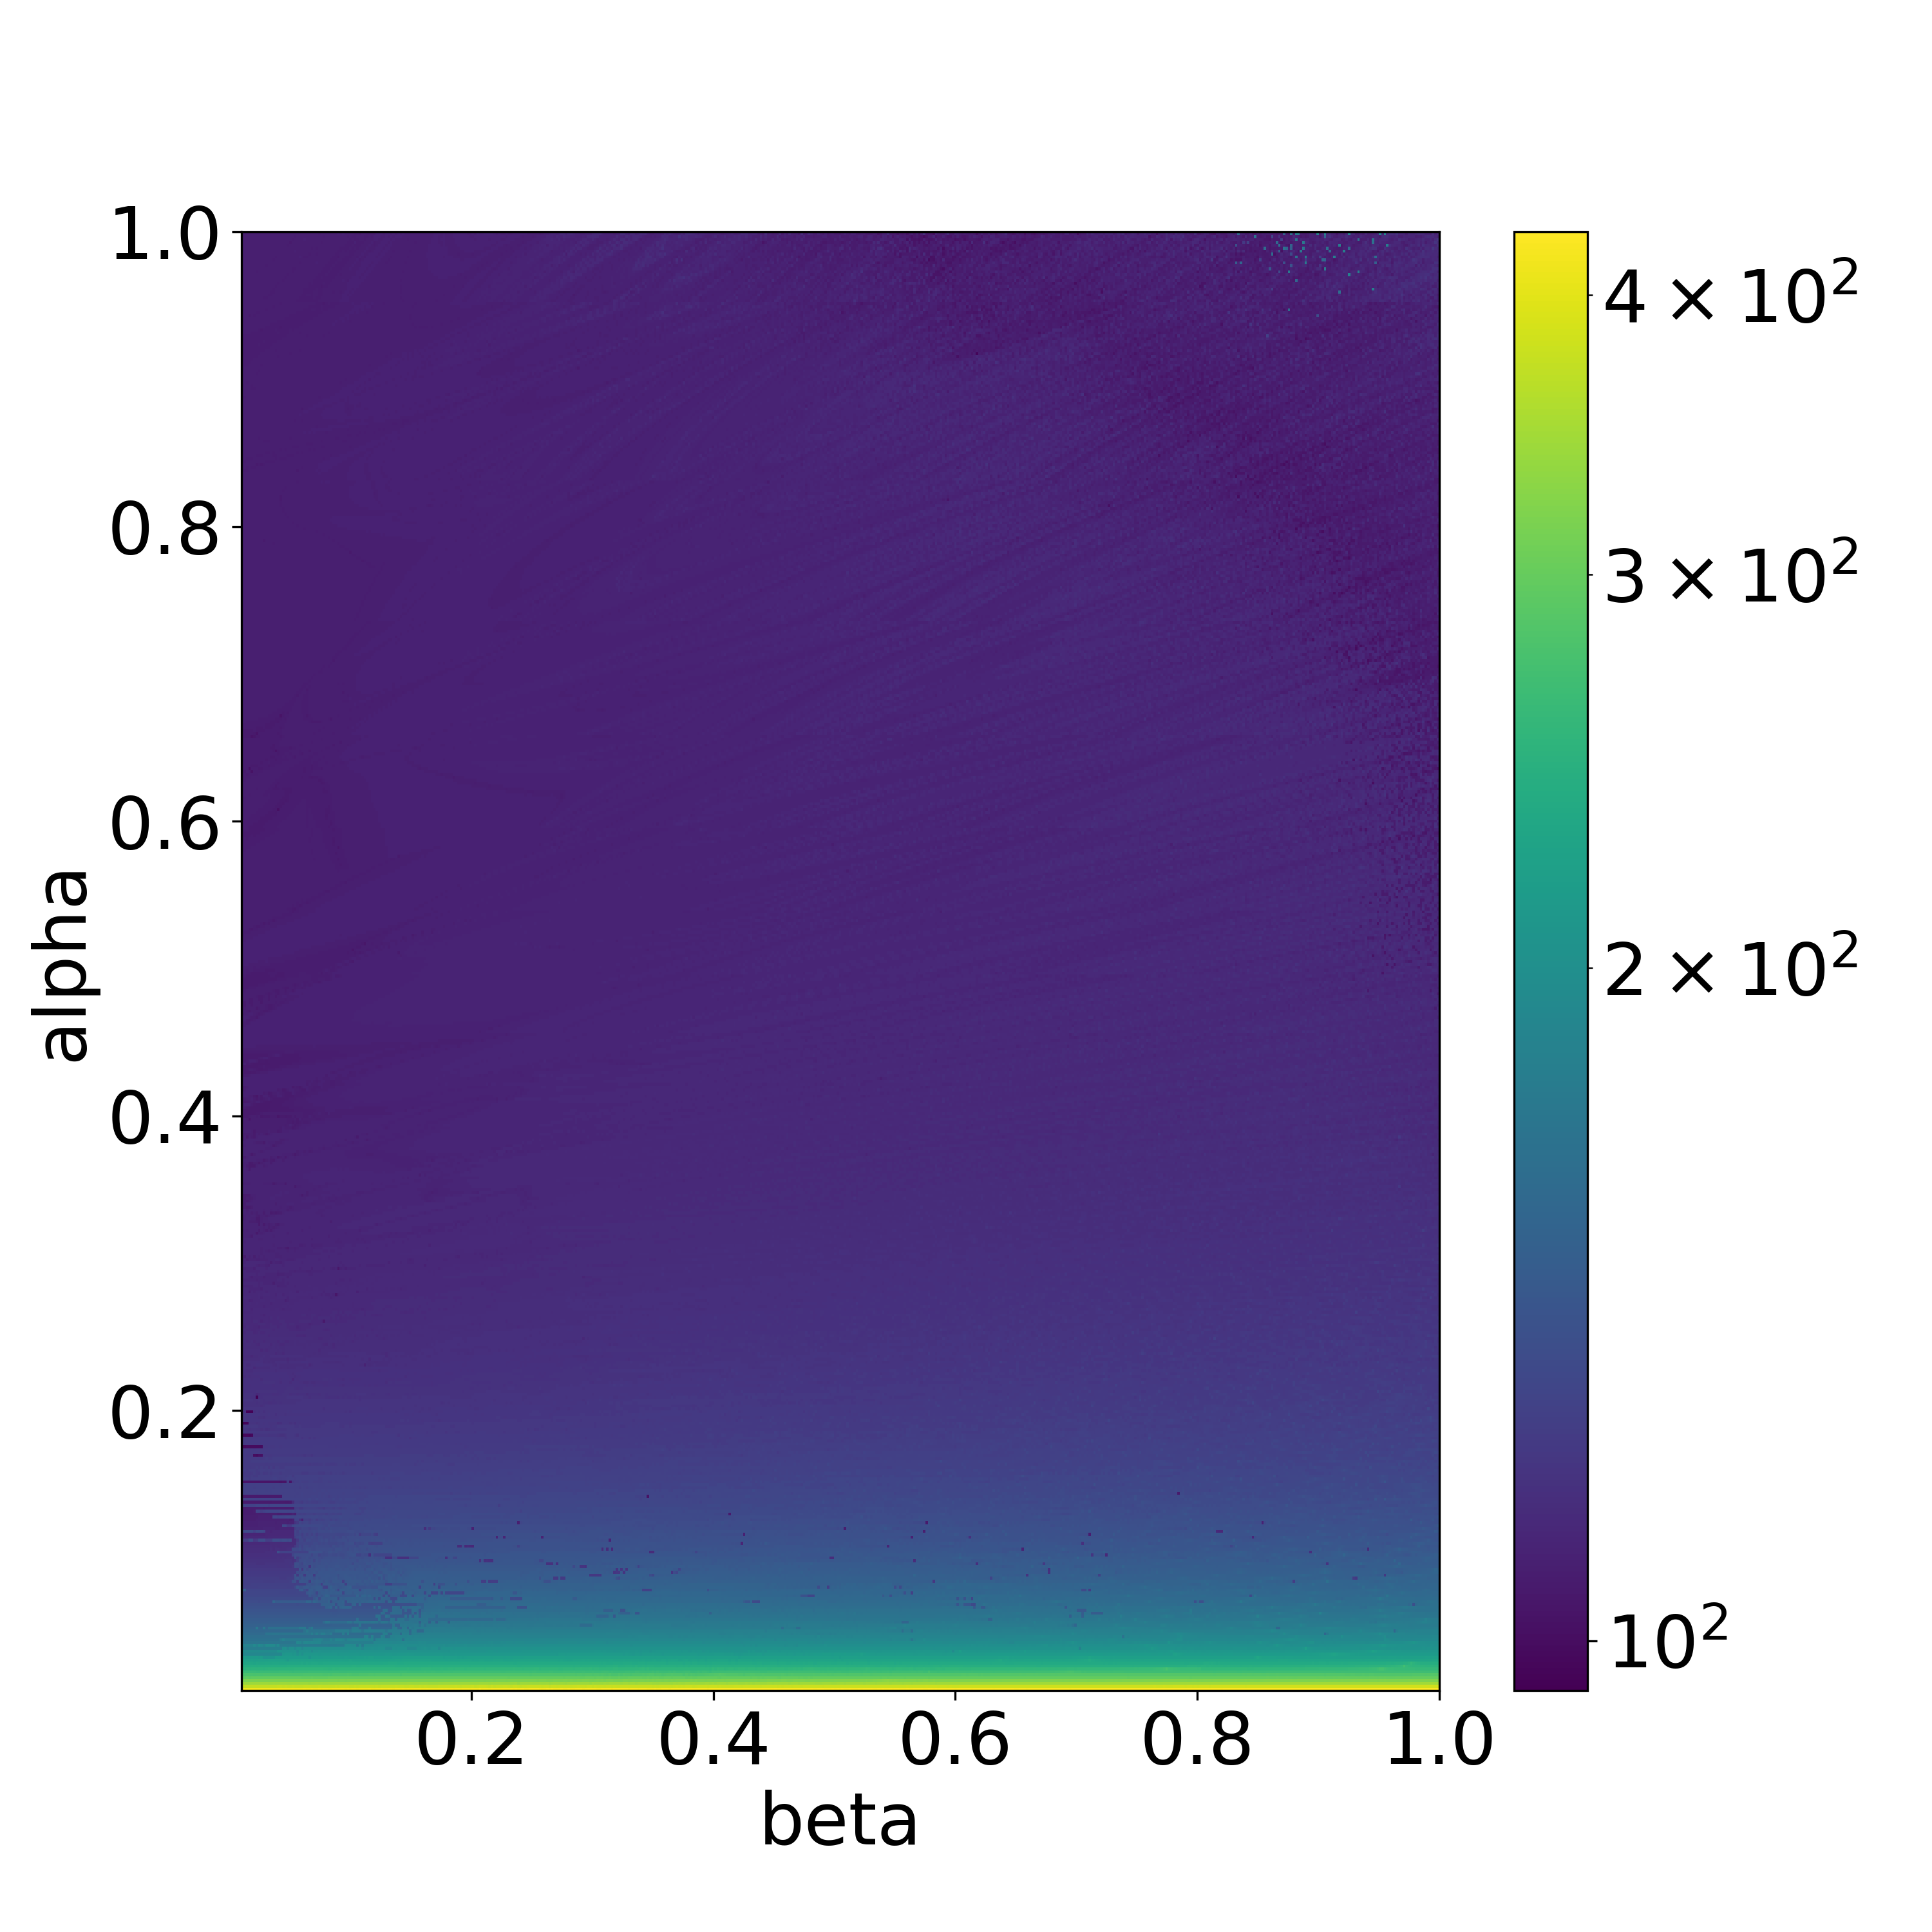
\includegraphics[width=1\textwidth]{images/analysis_RKF45_TS.png}
       	\subcaption{Number of required timesteps} 
        \label{fig:numberTimeStepsRKF45}
    \end{subfigure}
    \begin{subfigure}{0.32\textwidth}
    	\centering
    	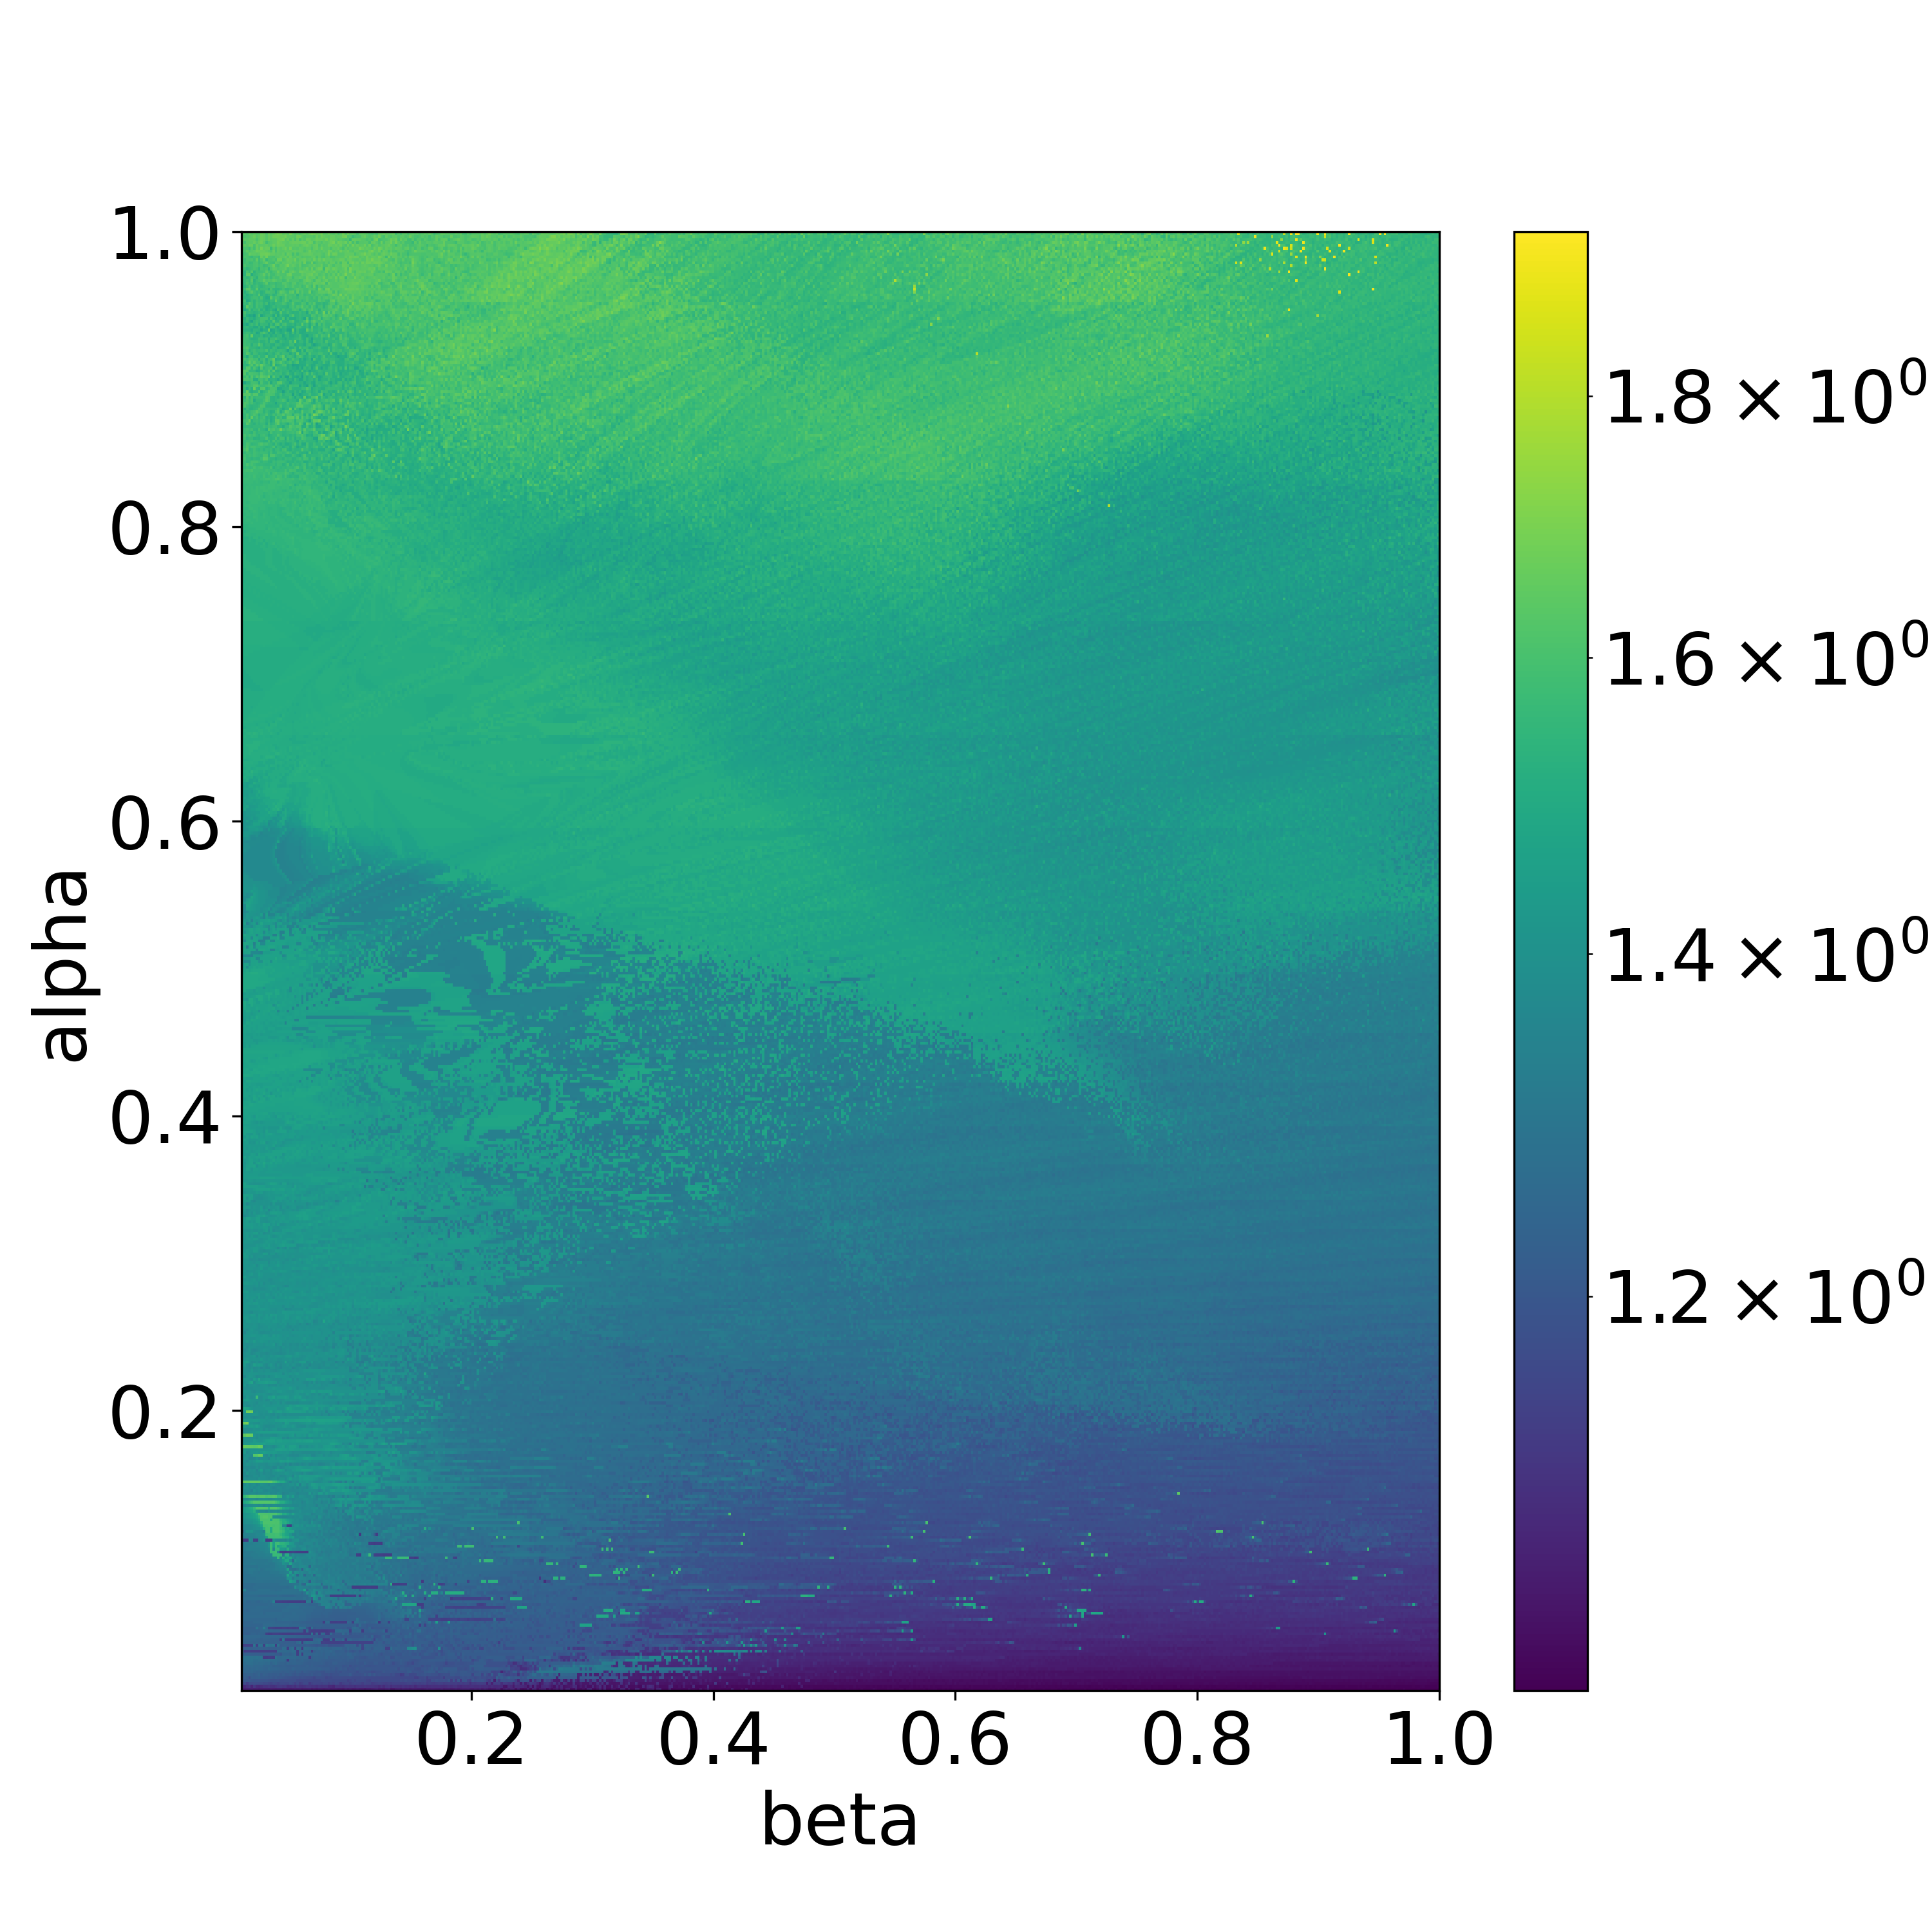
\includegraphics[width=1\textwidth]{images/analysis_RKF45_NI.png}
       	\subcaption{Average number of iterations per timestep} 
        \label{fig:numberIterationTSRKF45}
    \end{subfigure}
    \begin{subfigure}{0.32\textwidth}
    	\centering
    	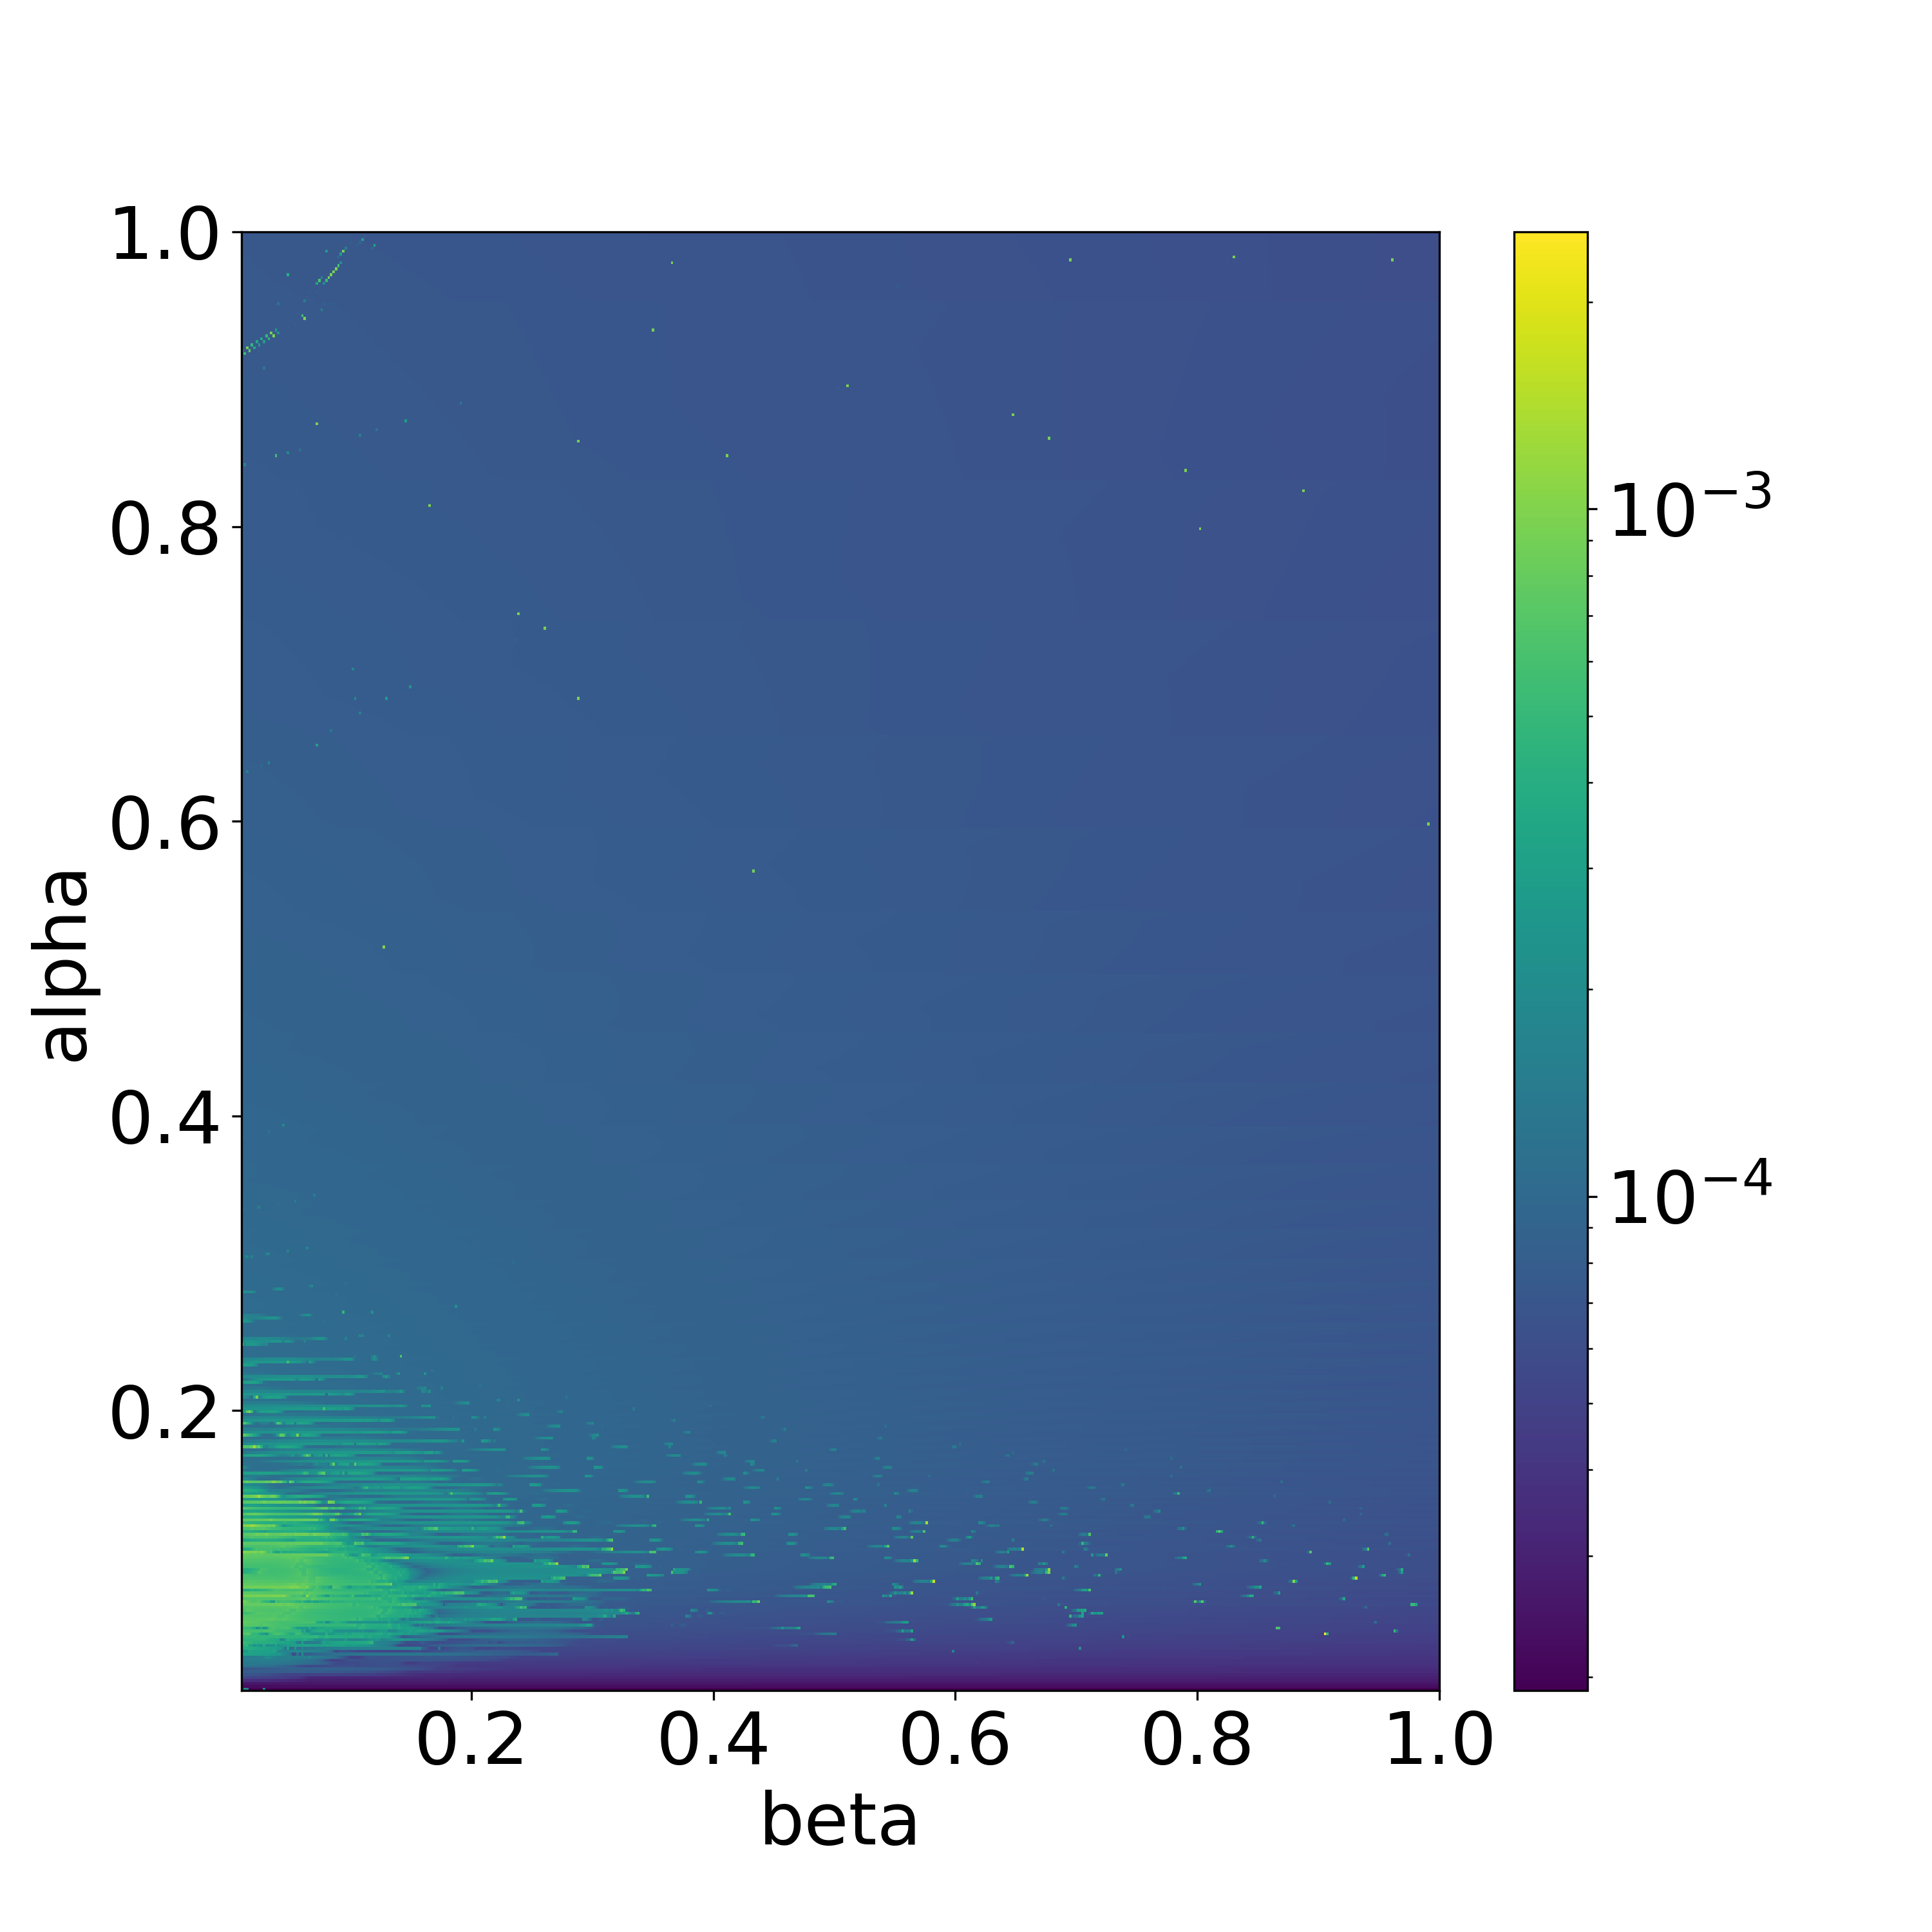
\includegraphics[width=1\textwidth]{images/analysis_RKF45_psi.png}
       	\subcaption{Absolute error of the variable $\psi$} 
        \label{fig:numberNumericalSchemeRKF45}
    \end{subfigure}
    \caption{Impact of the parameters $\alpha$ and $\beta$ of the PI controller on the number of required iterations to solve the model problem from \autoref{eq:first_DAE_ODE} using the explicit Runge-Kutta-Fehlberg method (\textbf{RKF45}) for a simulation time of $t=5.0s$}
    \label{fig:ParametersPIControllerRKF45}
\end{figure}


\begin{figure}[H]
    \centering
    \begin{subfigure}{0.32\textwidth}
    	\centering
    	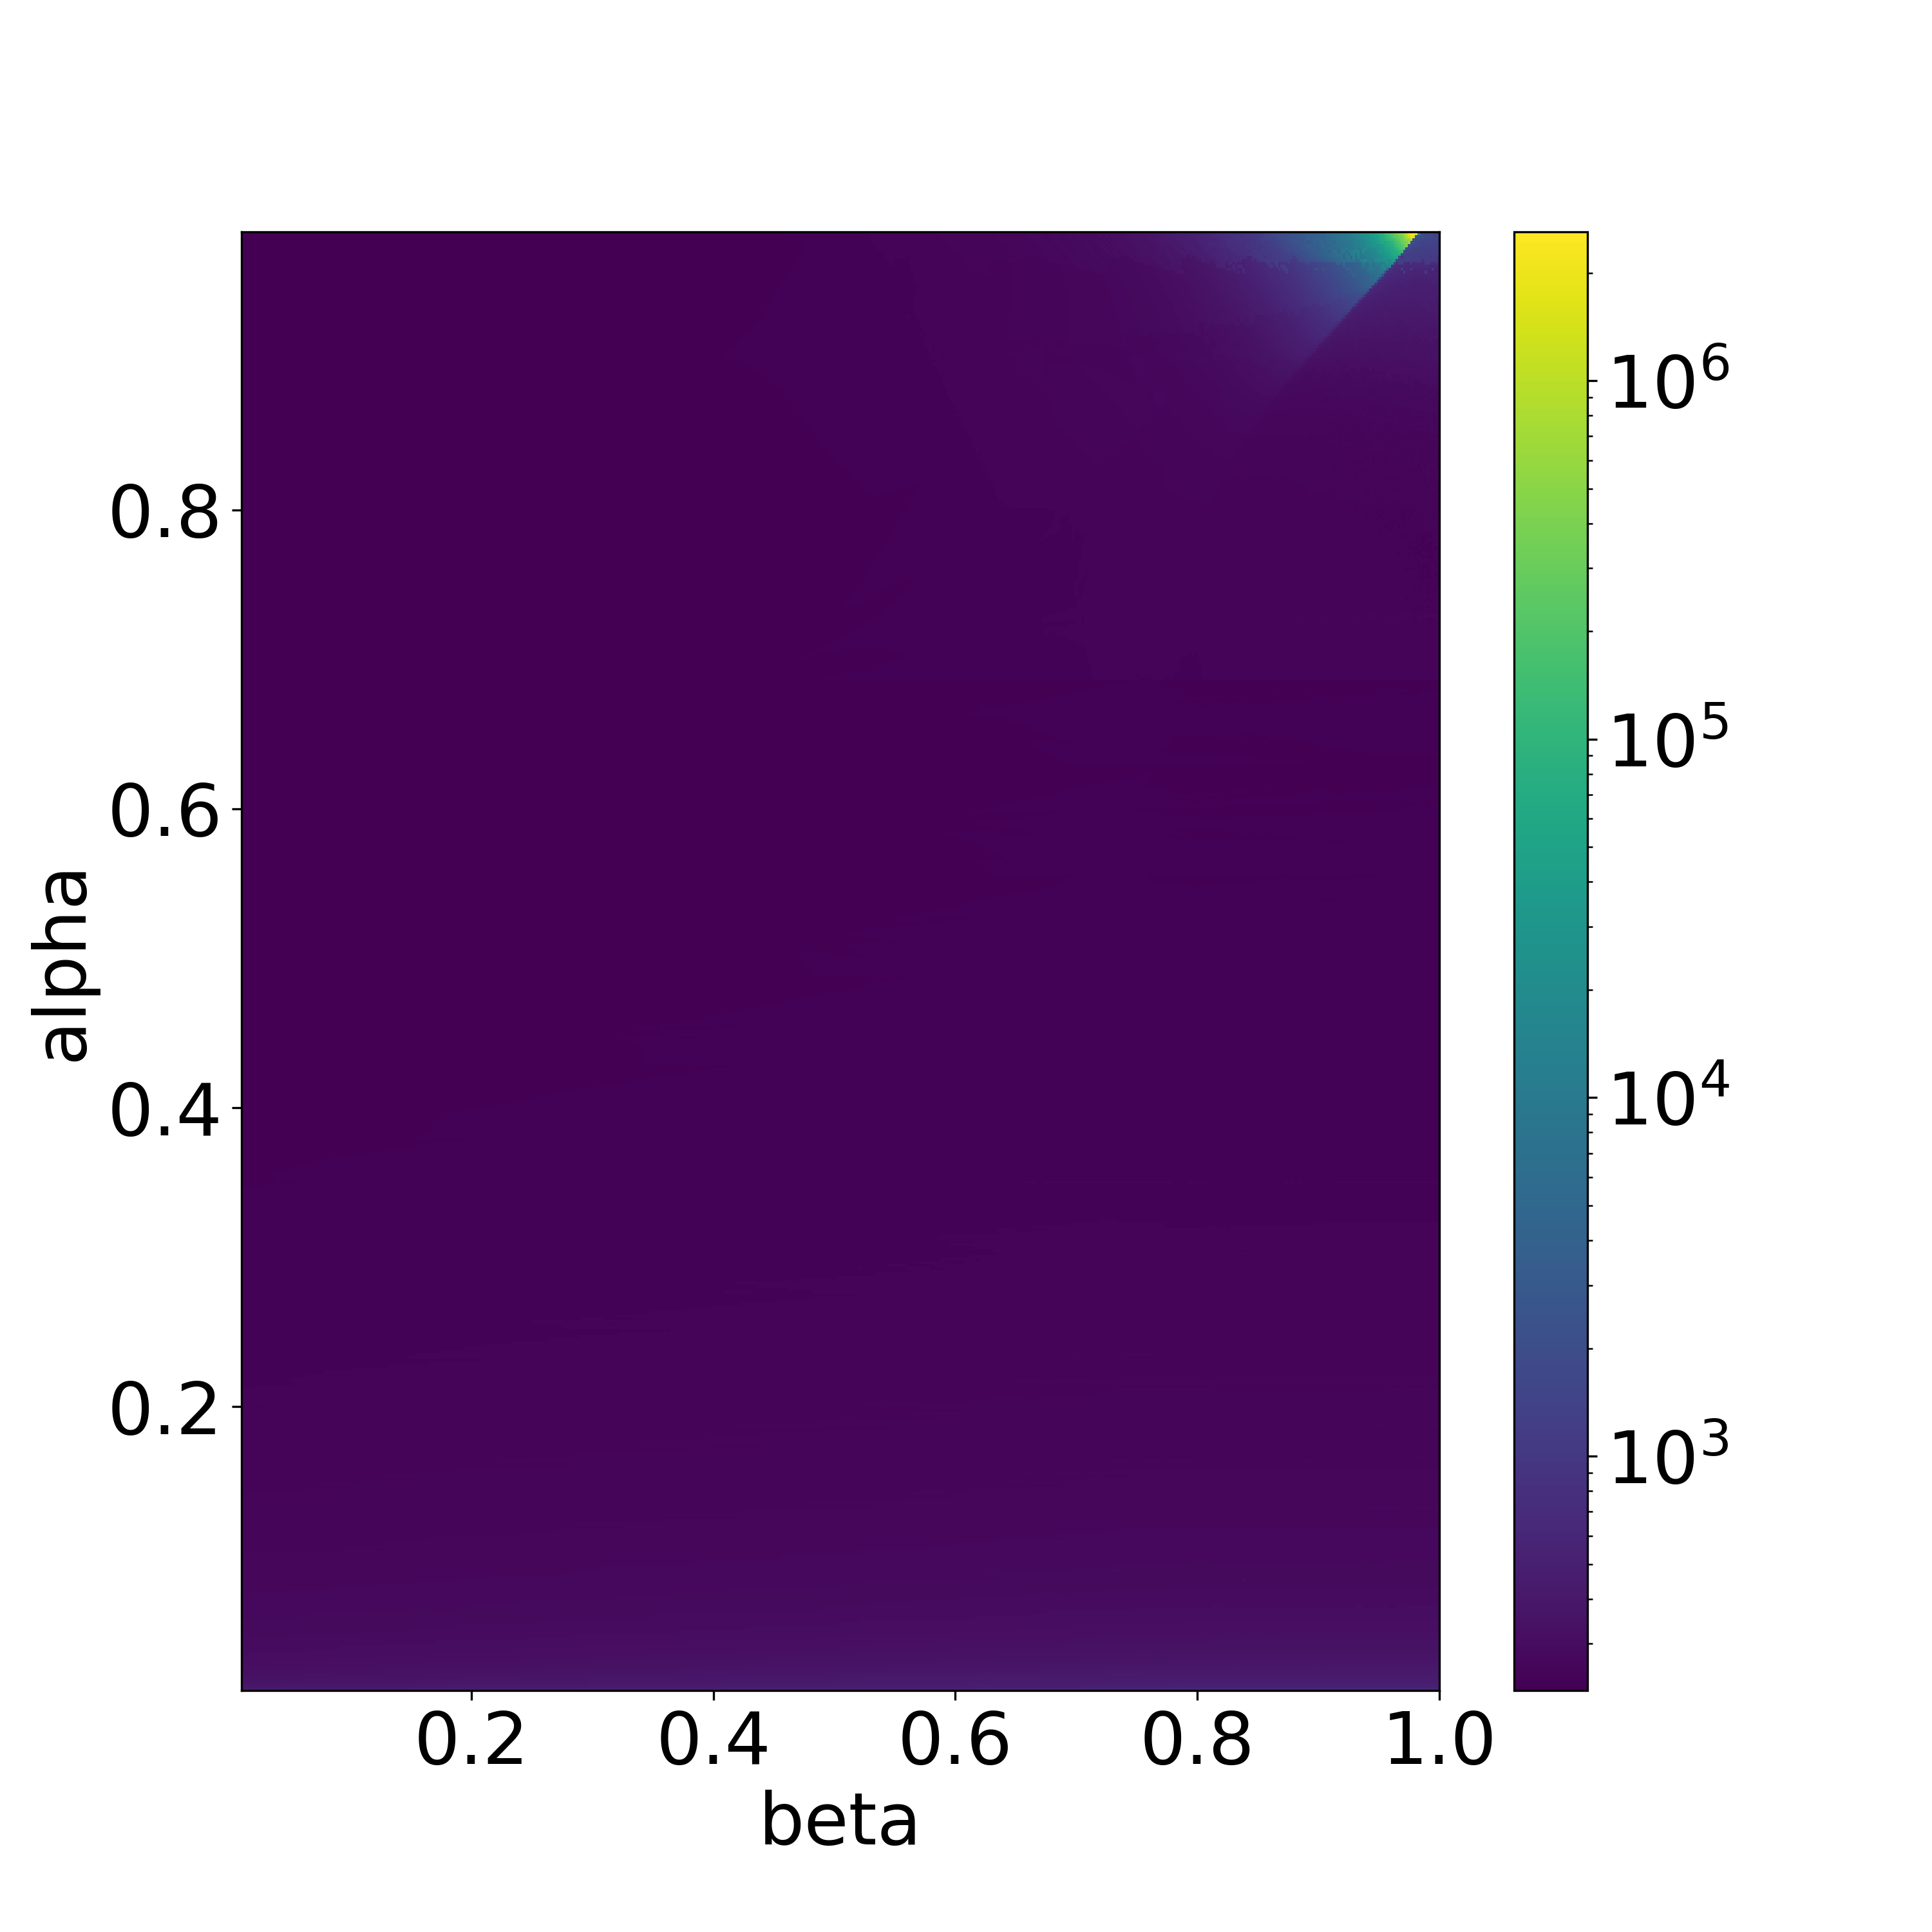
\includegraphics[width=1\textwidth]{images/analysis_BDF12_TS.png}
       	\subcaption{Number of required timesteps} 
        \label{fig:numberTimeStepsBDF12}
    \end{subfigure}
    \begin{subfigure}{0.32\textwidth}
    	\centering
    	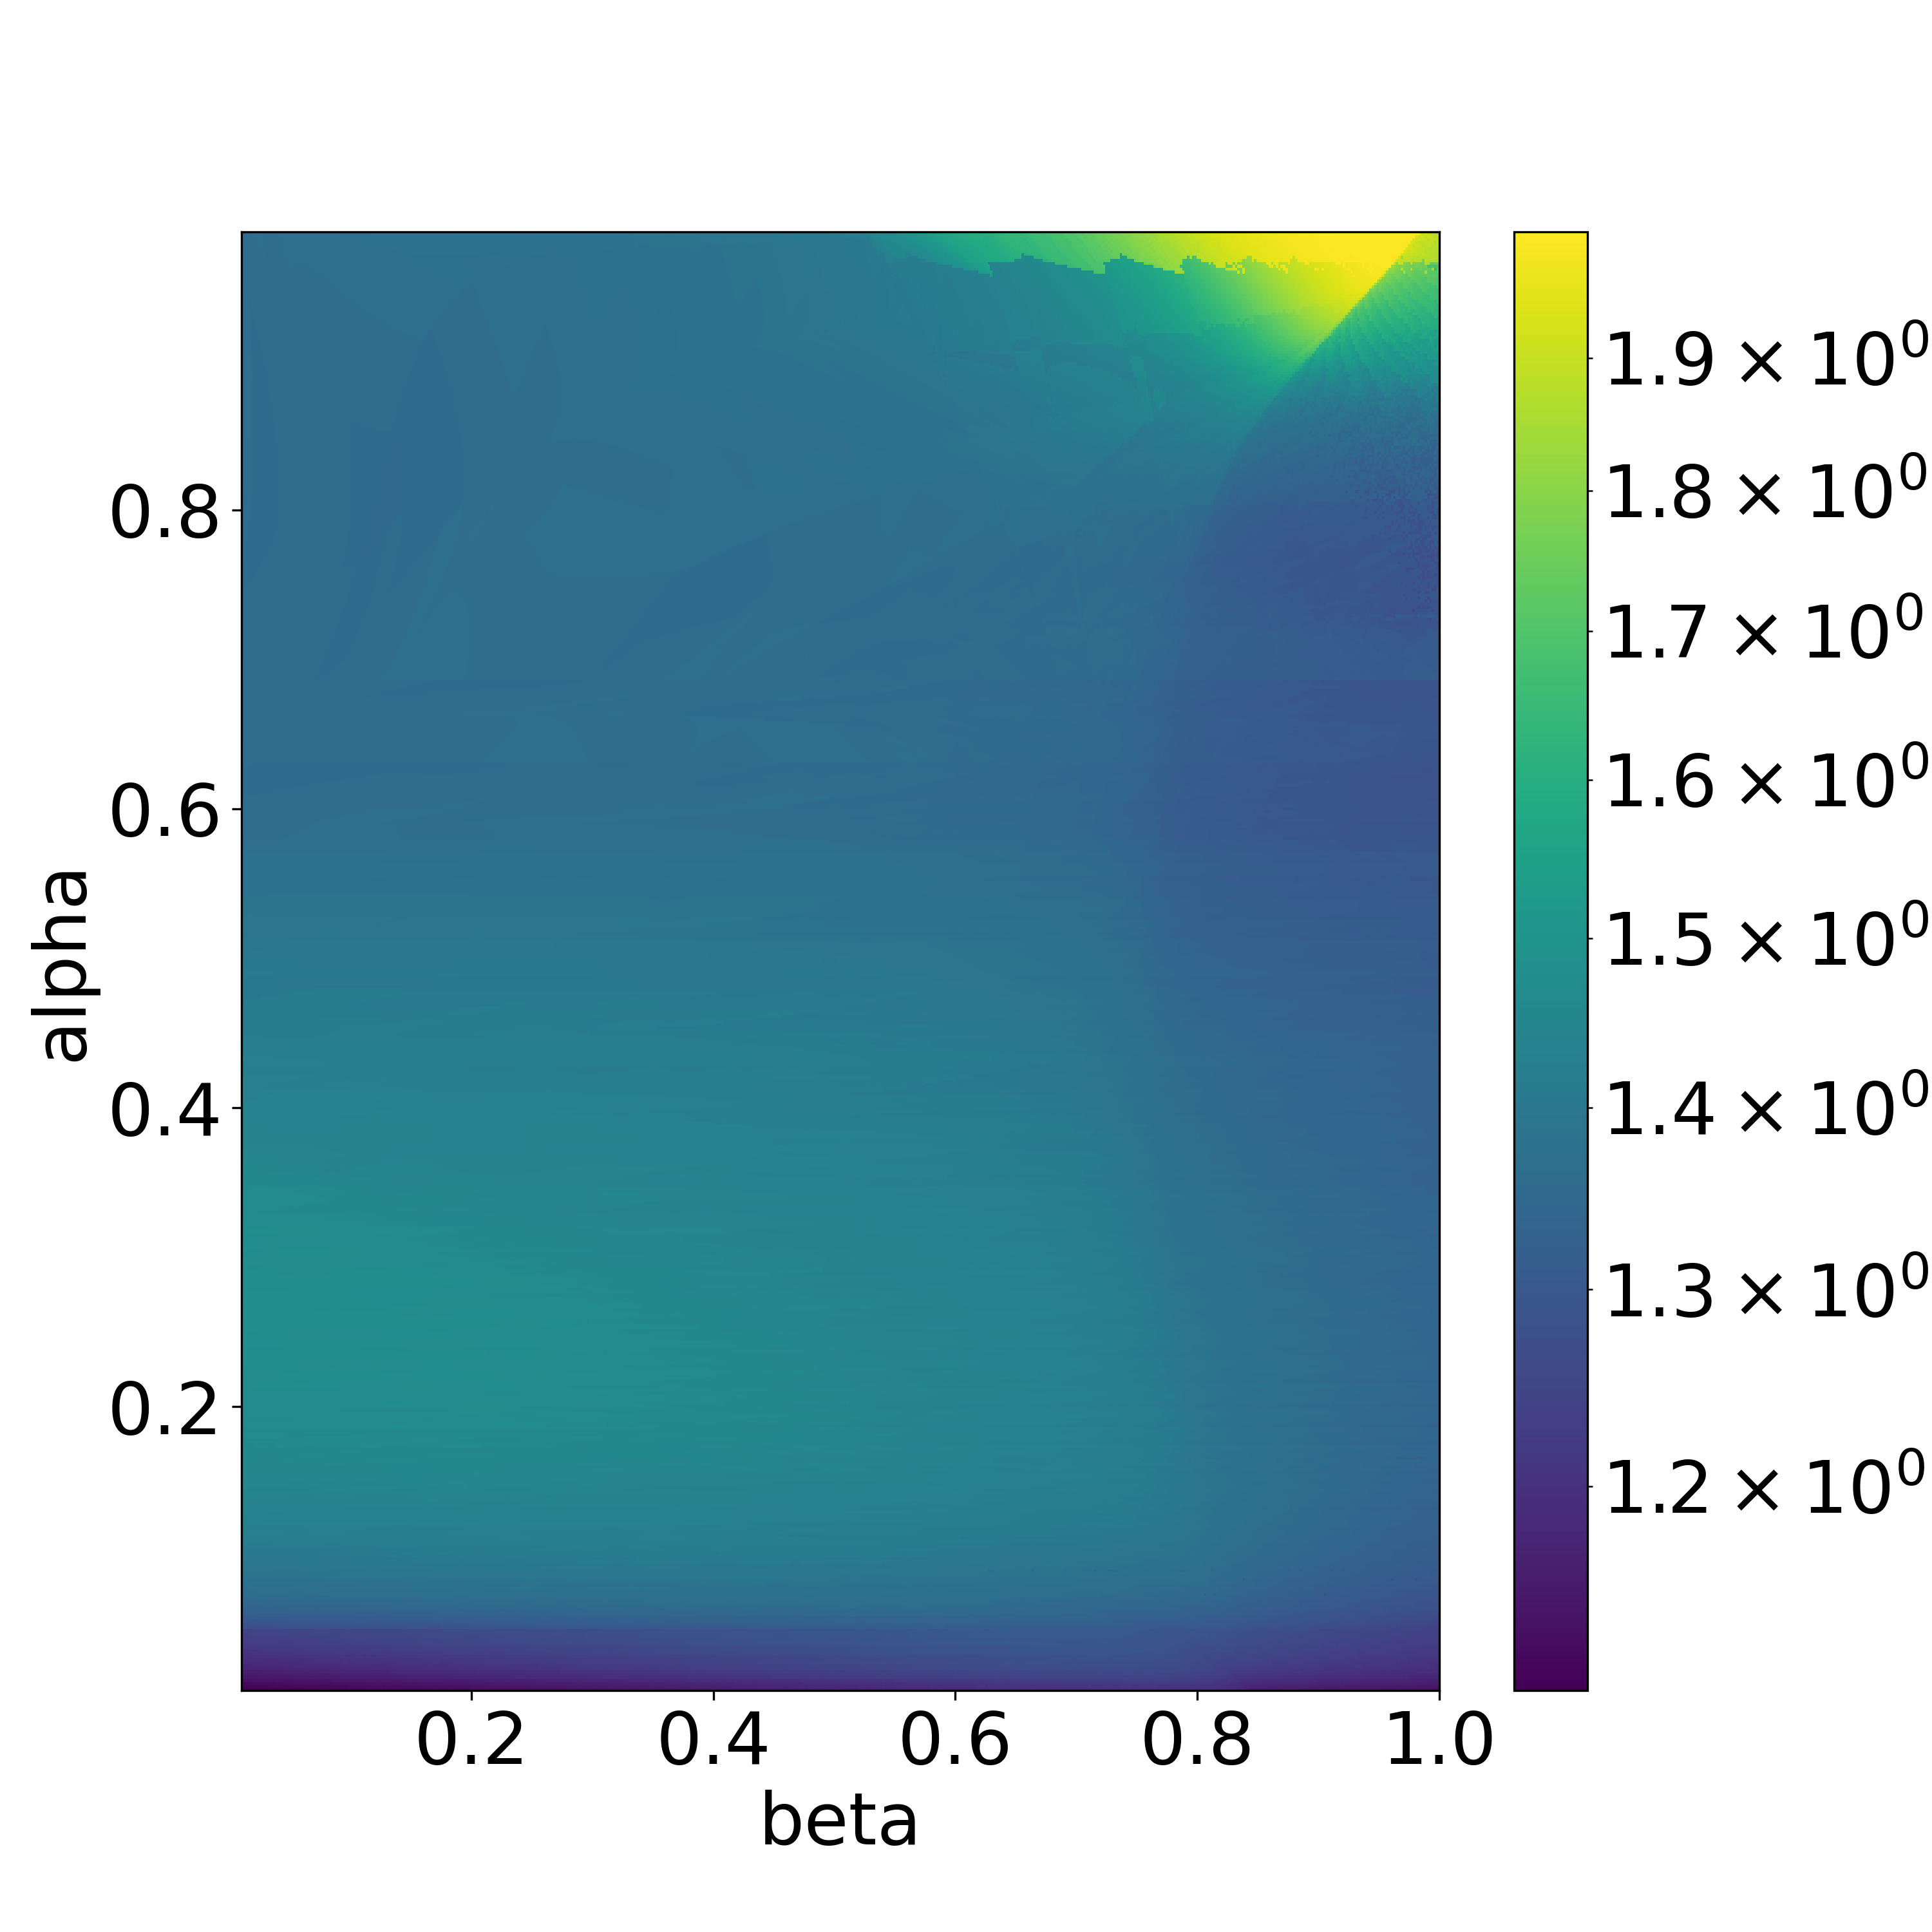
\includegraphics[width=1\textwidth]{images/analysis_BDF12_NI.png}
       	\subcaption{Average number of iterations per timestep} 
        \label{fig:numberIterationTSBDF12}
    \end{subfigure}
    \begin{subfigure}{0.32\textwidth}
    	\centering
    	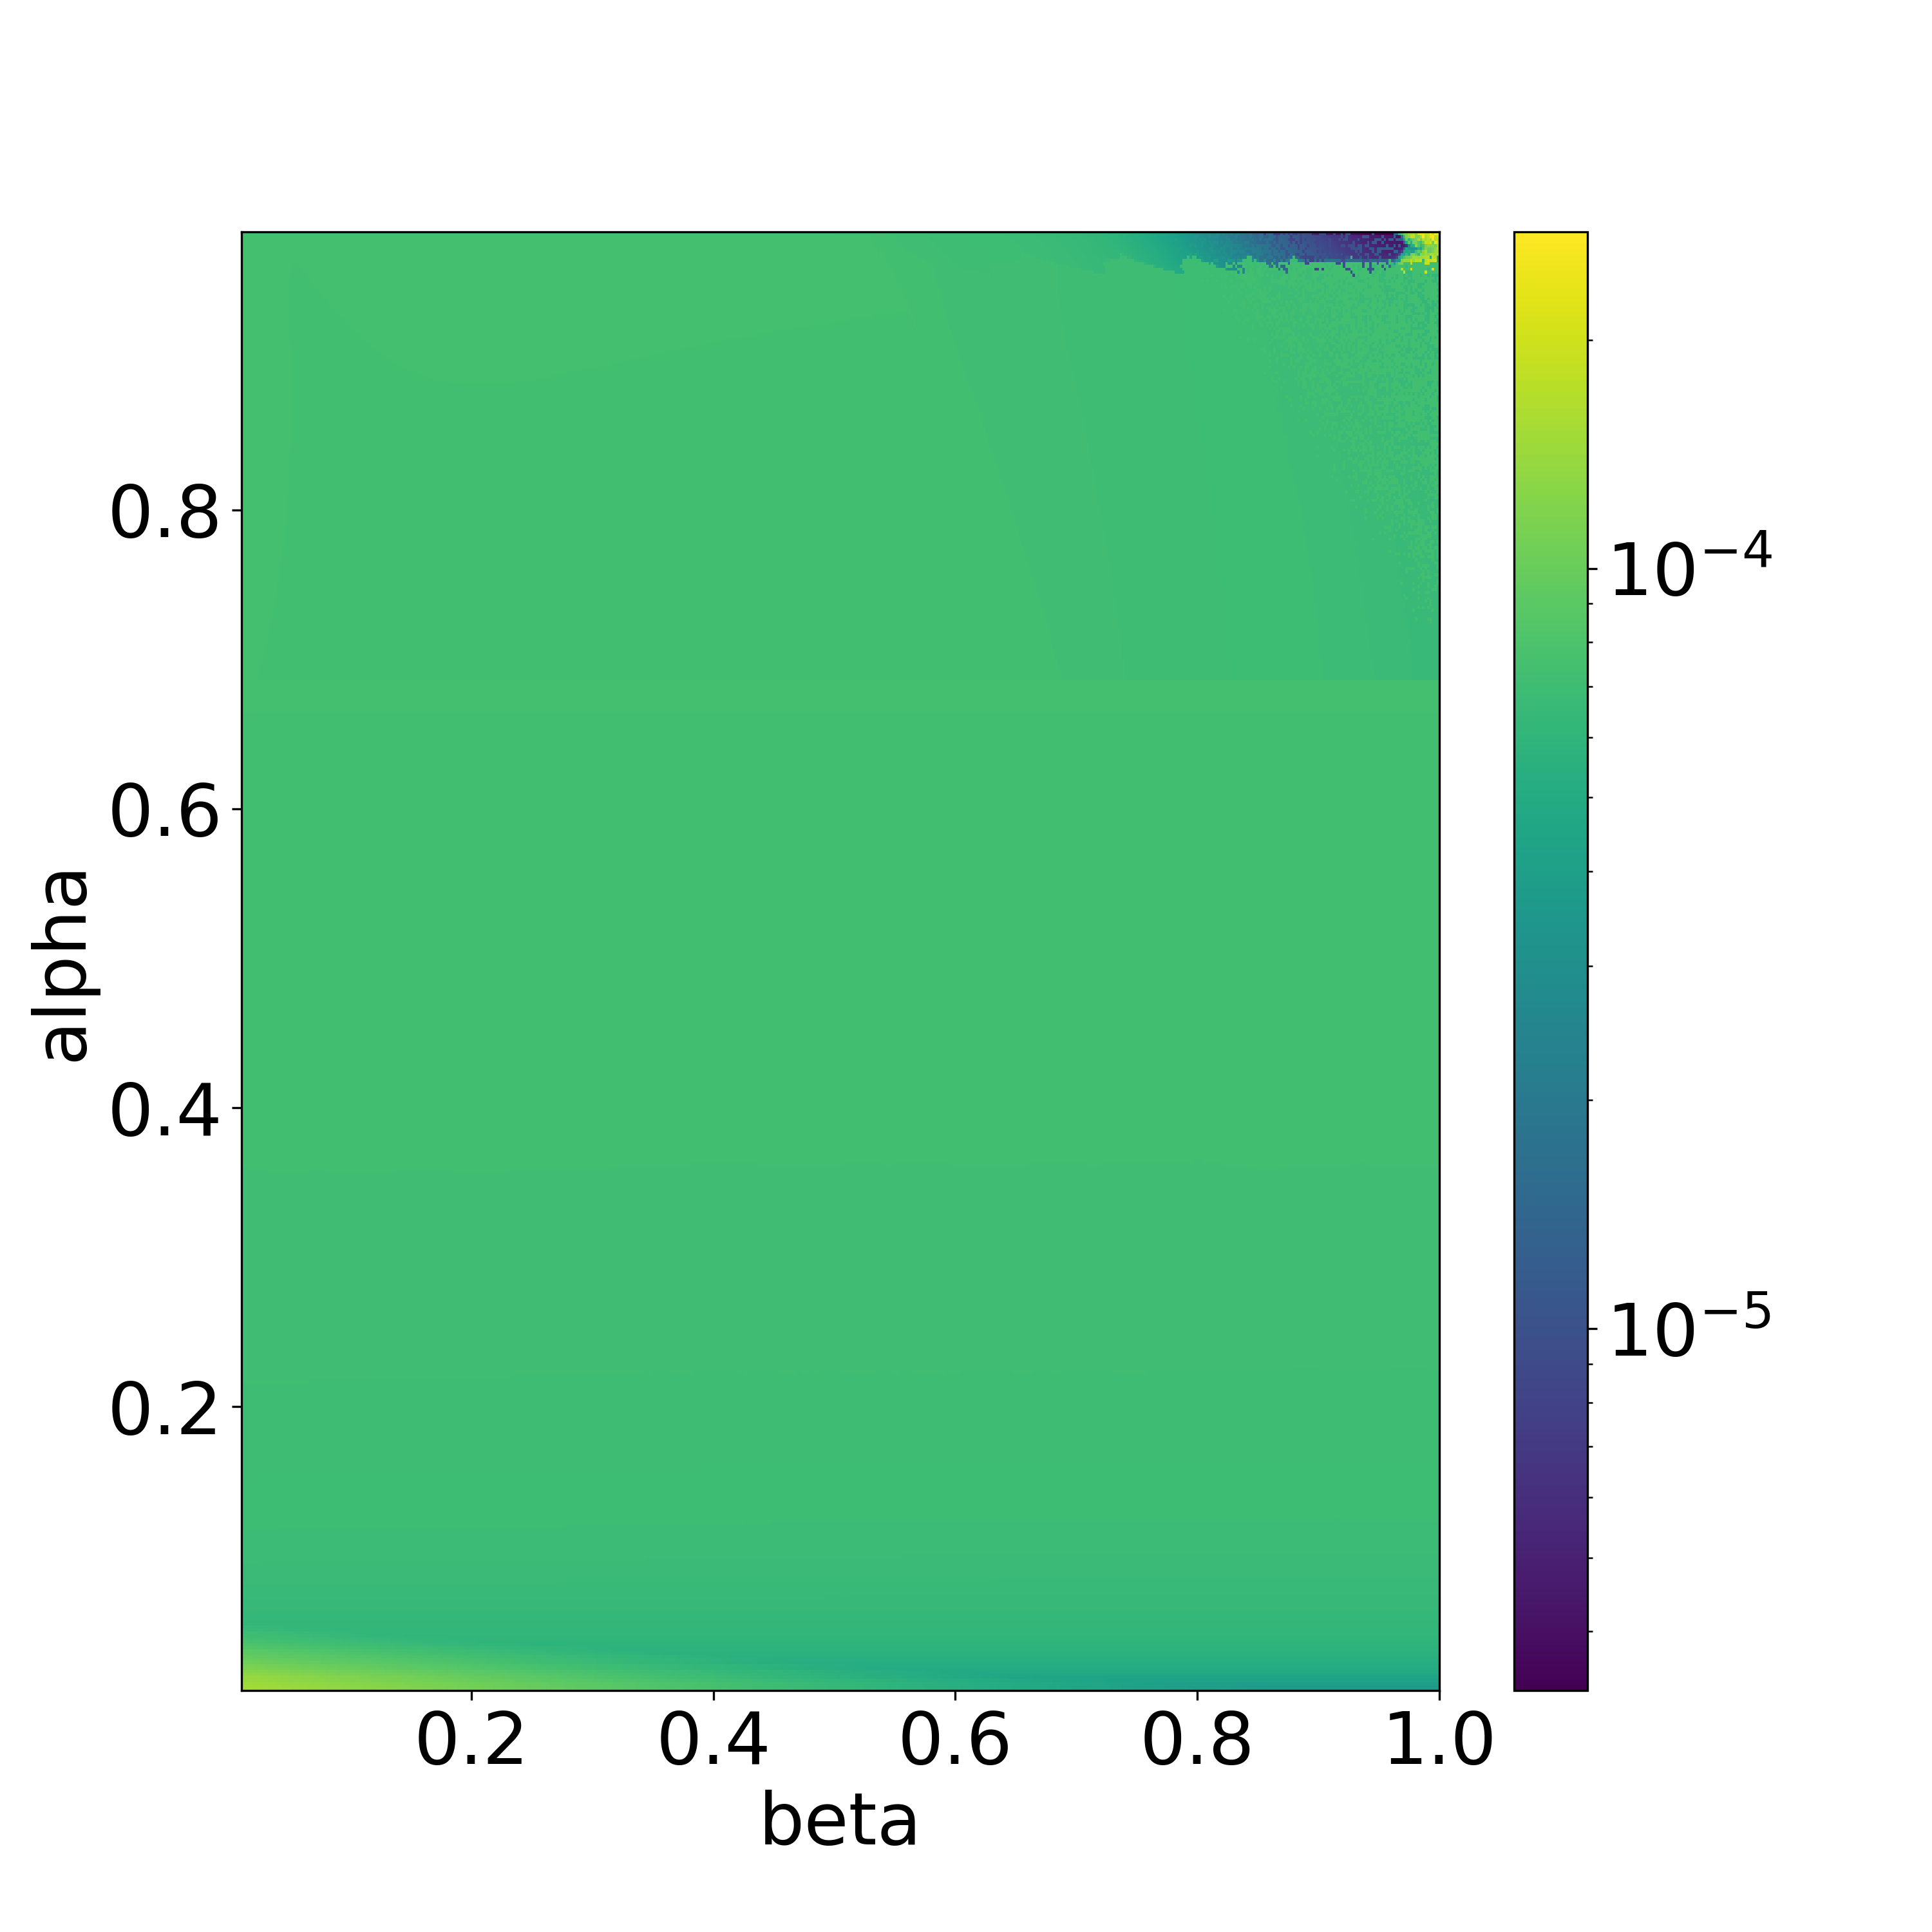
\includegraphics[width=1\textwidth]{images/analysis_BDF12_psi.png}
       	\subcaption{Absolute error of the variable $\psi$} 
        \label{fig:numberNumericalSchemeBDF12}
    \end{subfigure}
    \caption{Impact of the parameters $\alpha$ and $\beta$ of the PI controller on the number of required iterations to solve the model problem from \autoref{eq:first_DAE_ODE} using the implicit BDF method of first order (\textbf{BDF12}) for a simulation time of $t=5.0s$}
    \label{fig:ParametersPIControllerBDF12}
\end{figure}


\begin{figure}[H]
    \centering
    \begin{subfigure}{0.32\textwidth}
    	\centering
    	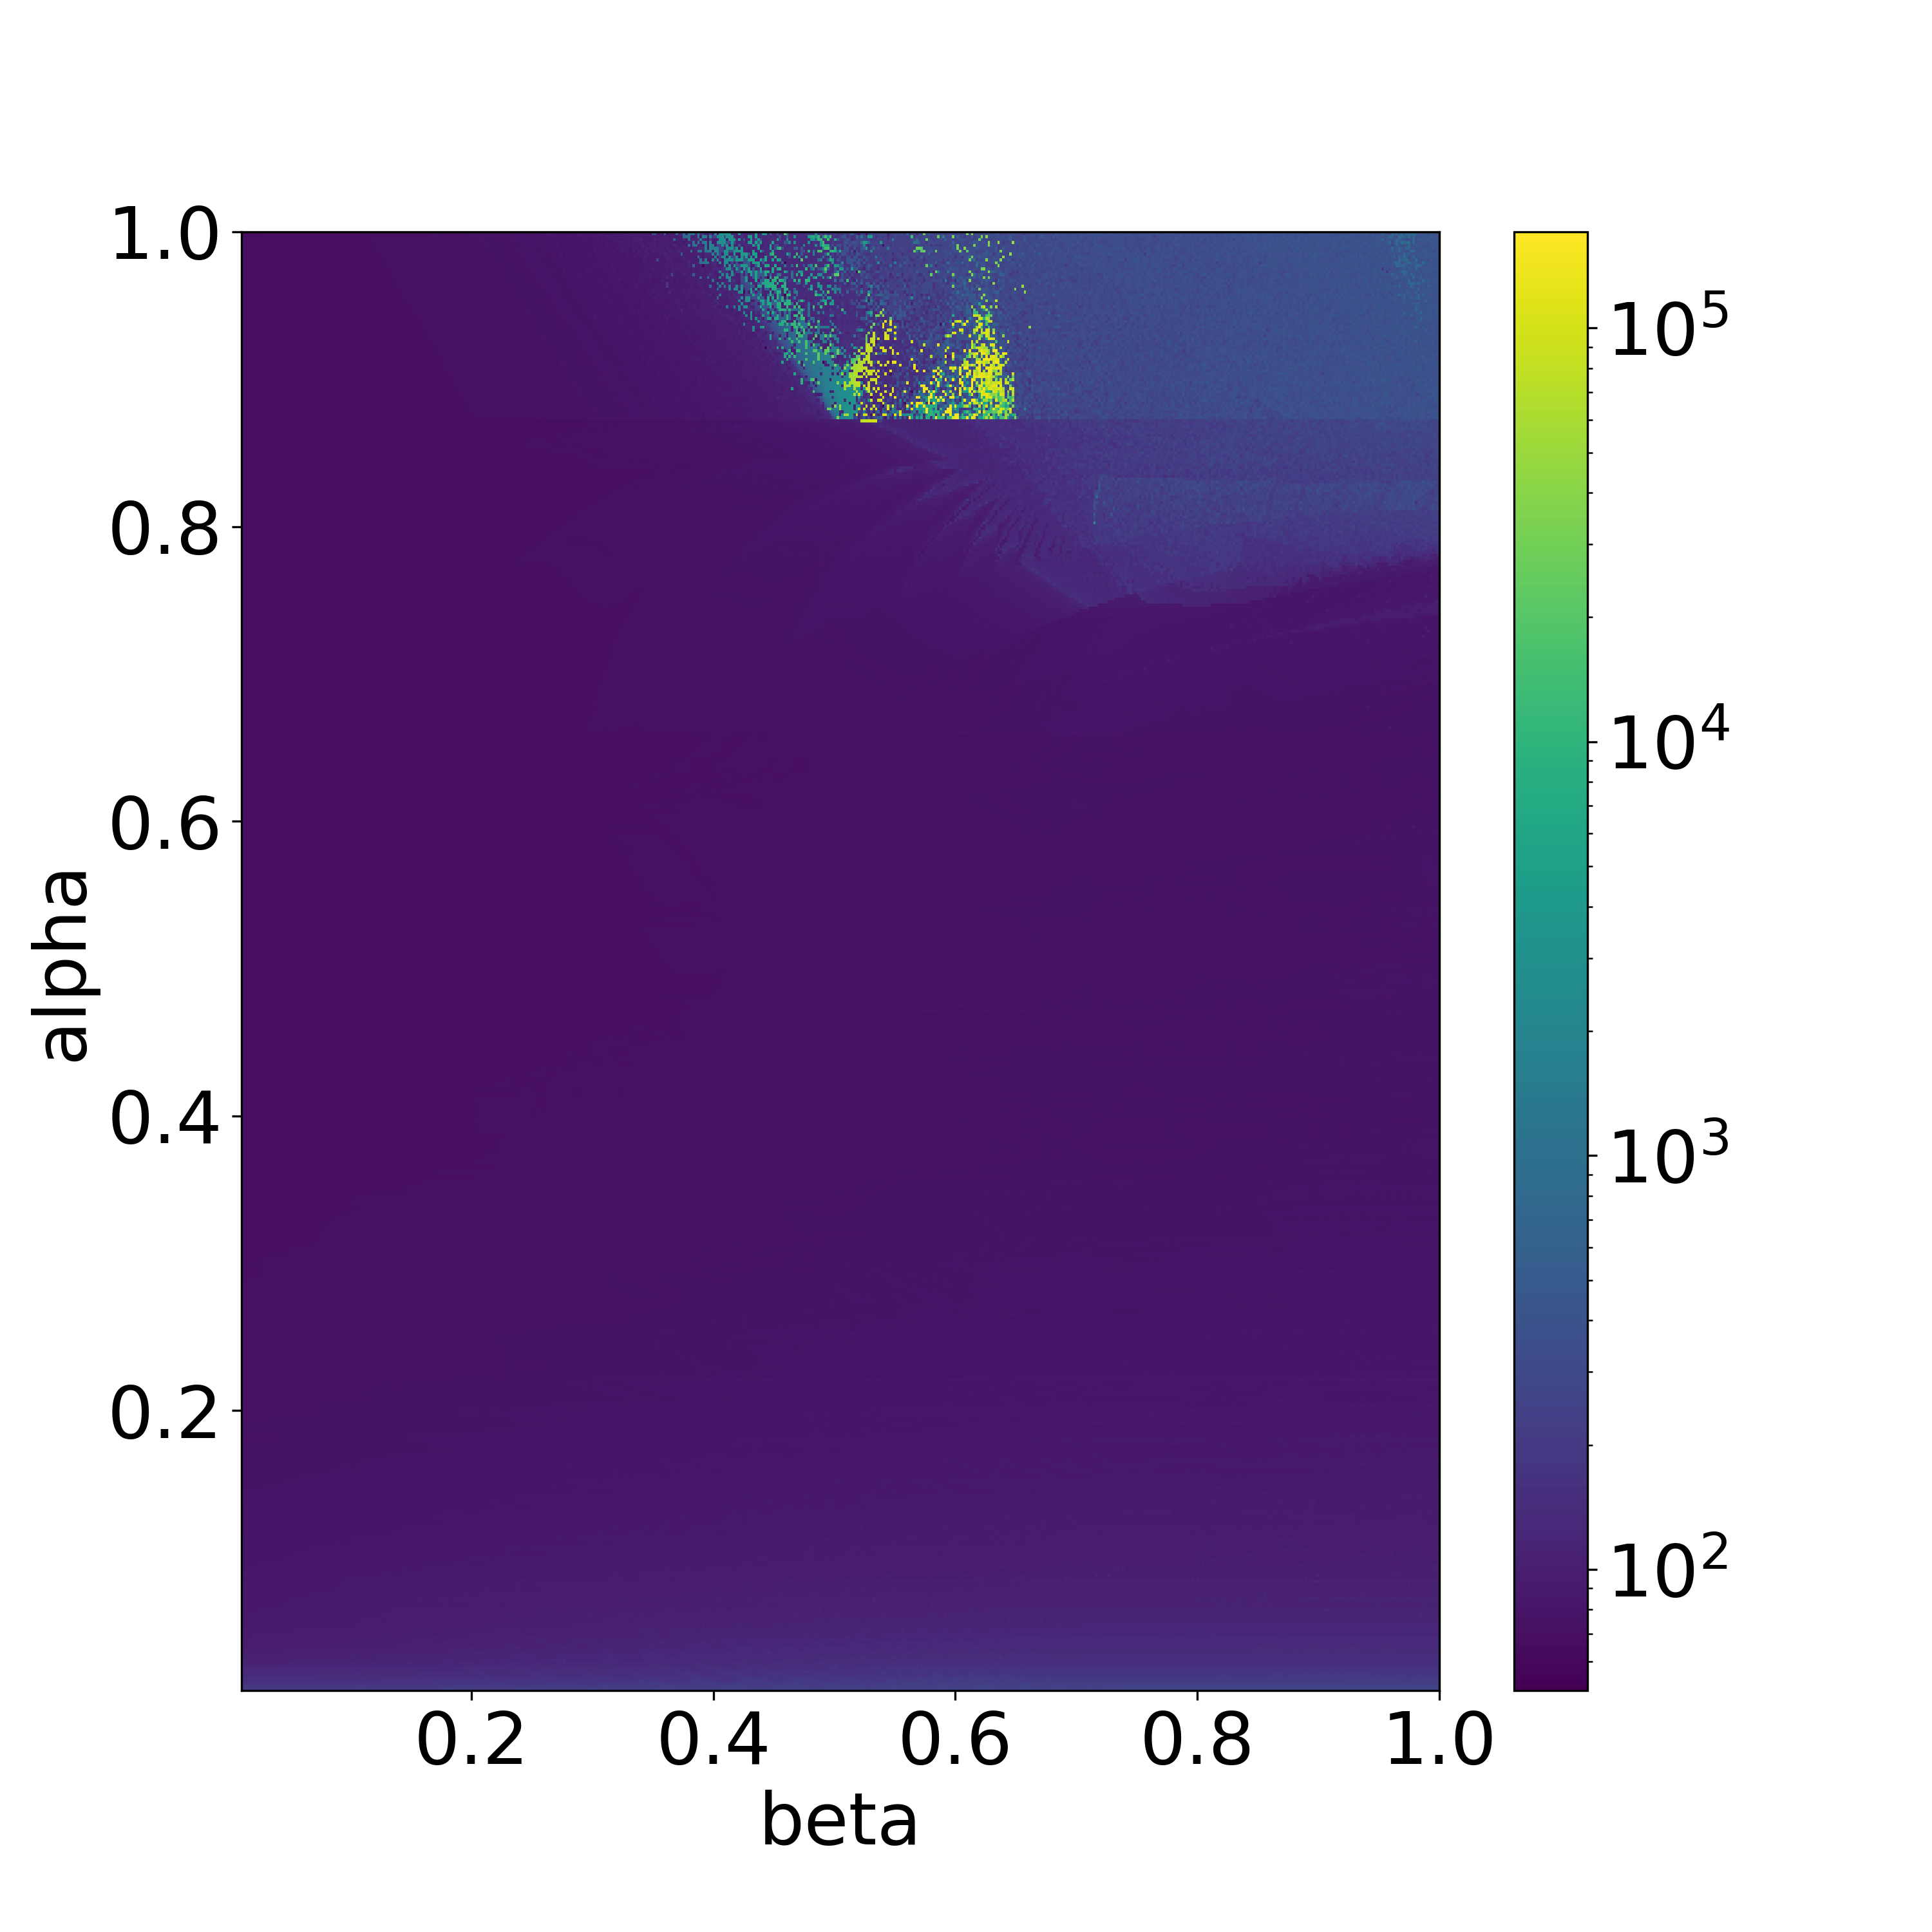
\includegraphics[width=1\textwidth]{images/analysis_BDF23_TS.png}
       	\subcaption{Number of required timesteps} 
        \label{fig:numberTimeStepsBDF23}
    \end{subfigure}
    \begin{subfigure}{0.32\textwidth}
    	\centering
    	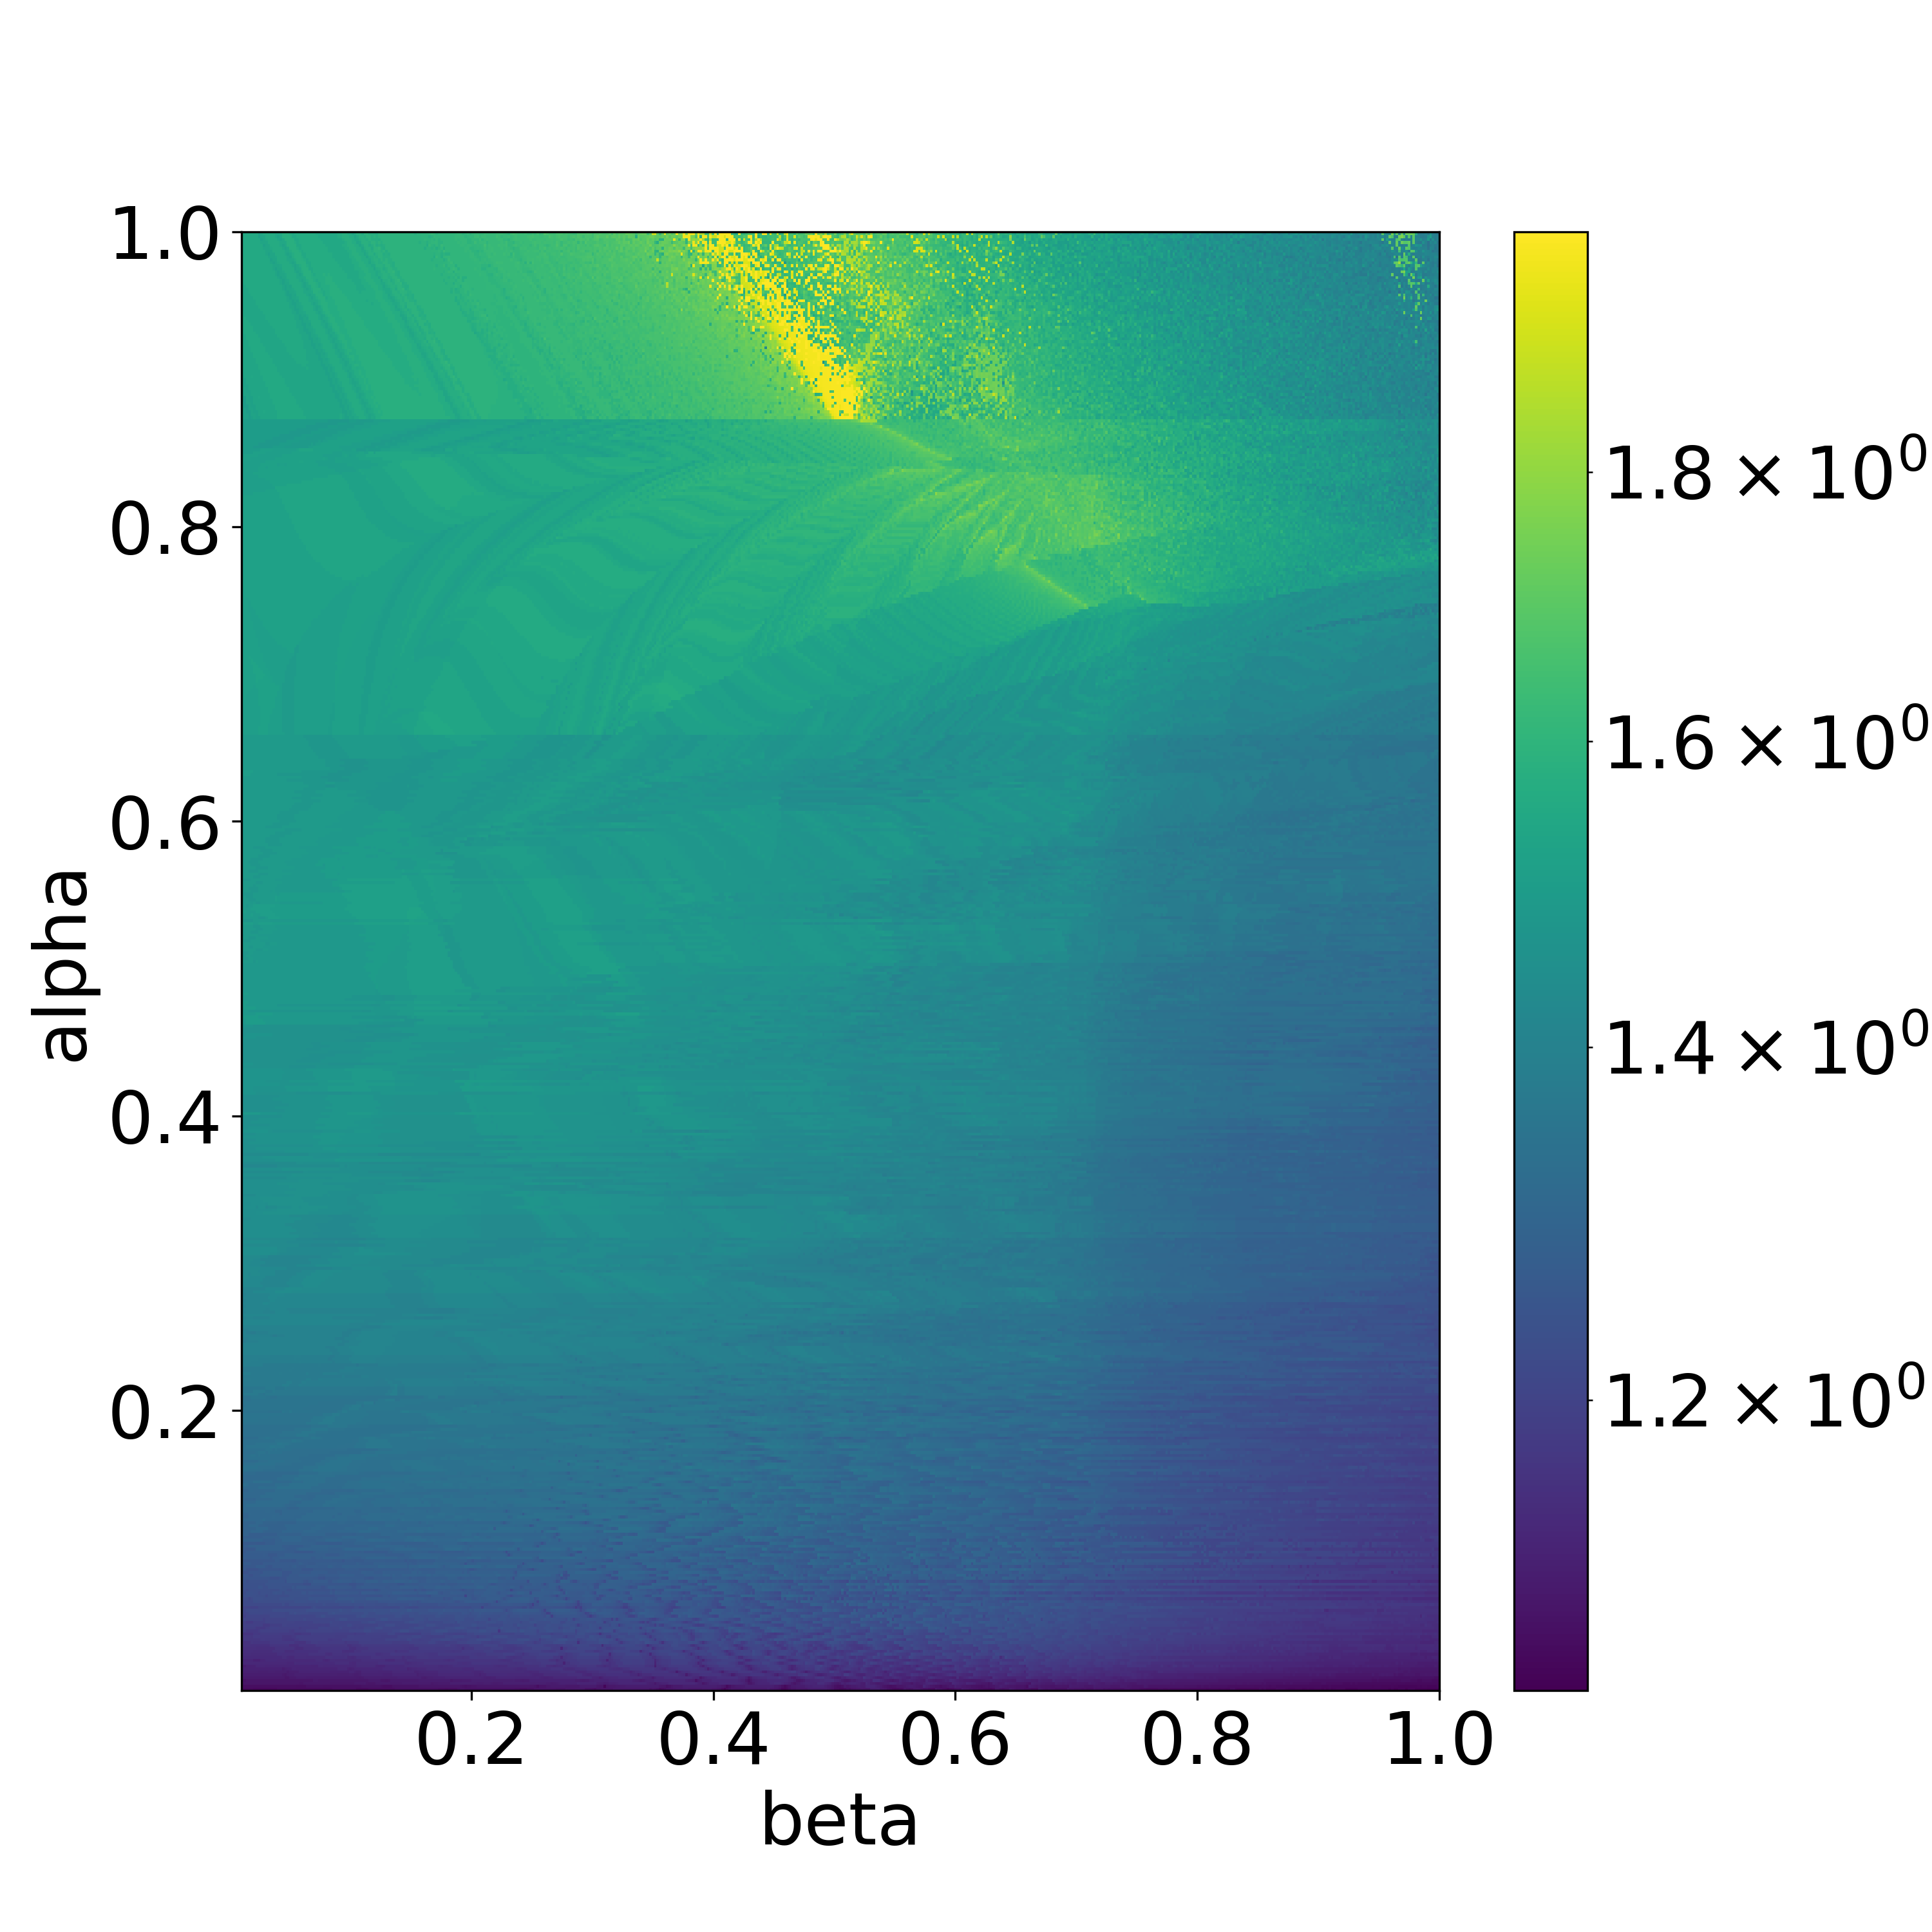
\includegraphics[width=1\textwidth]{images/analysis_BDF23_NI.png}
       	\subcaption{Average number of iterations per timestep} 
        \label{fig:numberIterationTSBDF23}
    \end{subfigure}
    \begin{subfigure}{0.32\textwidth}
    	\centering
    	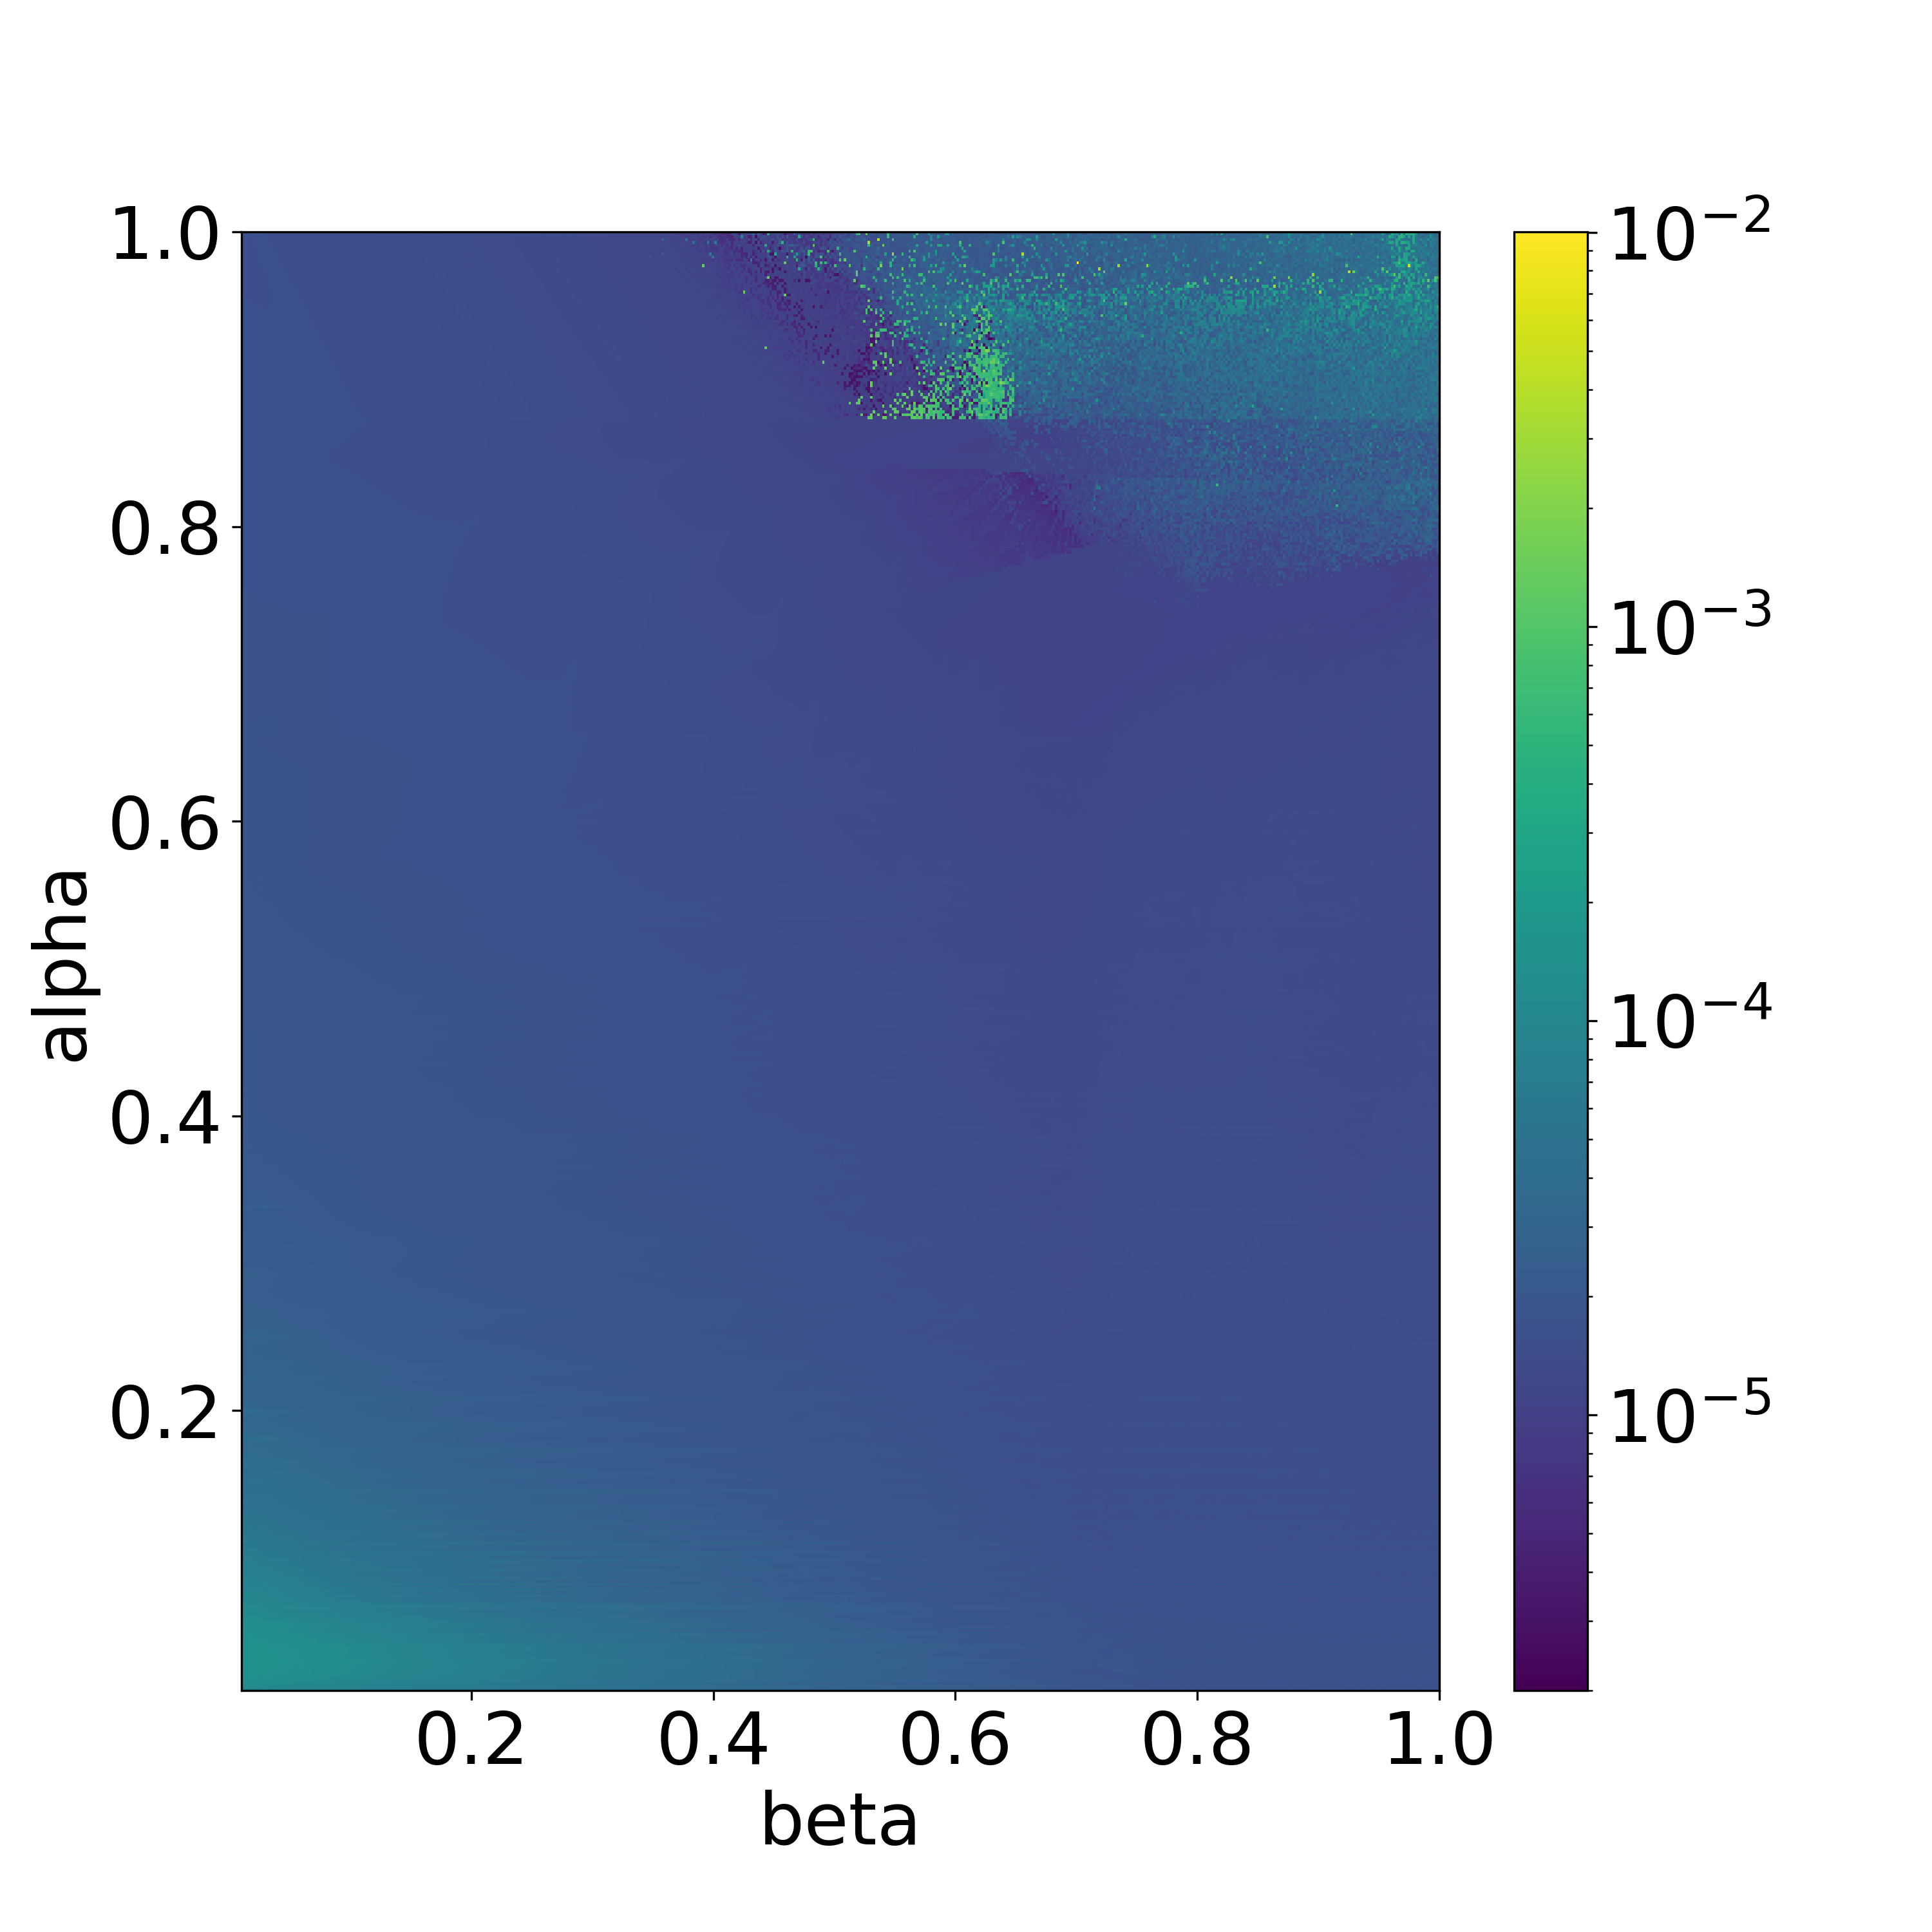
\includegraphics[width=1\textwidth]{images/analysis_BDF23_psi.png}
       	\subcaption{Absolute error of the variable $\psi$} 
        \label{fig:numberNumericalSchemeBDF23}
    \end{subfigure}
    \caption{Impact of the parameters $\alpha$ and $\beta$ of the PI controller on the number of required iterations to solve the model problem from \autoref{eq:first_DAE_ODE} using the implicit BDF method of second order (\textbf{BDF23}) for a simulation time of $t=5.0s$}
    \label{fig:ParametersPIControllerBDF23}
\end{figure}

We chose as parameters: 
\begin{itemize}
    \item for \textbf{RKF45}: $\alpha=0.4$ and $\beta=0.6$
    \item for \textbf{BDF12}: $\alpha=0.9$ and $\beta=0.4$
    \item for \textbf{BDF23}: $\alpha=0.9$ and $\beta=0.4$
\end{itemize}

---Put some more explanations here --- \\
---Find the balance between number of iterations and accuracy --- \\
---Numerical instabilities for the implicit methods for high values of $\alpha$ and $\beta$ --- \\
failure of the error estimate? too small timesteps? \\ 

\section{Comparison of the Numerical Schemes}
So far, one explicit (RKF45) and two implicit (BDF12, BDF23) numerical solvers have been implemented for the initial DAE in \autoref{eq:first_DAE_algeb} and their ideal parameter choice for their use with a PI controller has been discussed. Now, the quality of the solutions is compared. \\
Again, the allowed tolerance of the PI controller is set to $\epsilon=1\cdot 10^{-6}$. The method of the manufactured solutions is chosen to have an analytical solution against which numerical computations can be compared. The parameters $t_e$ and $t_w$ are chosen in a way that the velocity is initially close to zero and increases to 1 over the time span of one second at the middle of the simulation time. \autoref{fig:timeEvolutionValues} depicts the solution variables $\psi$ and $V$ over time for all three solvers. The expected form of the $\text{atan}$ function centered around $2.5$ for the velocity is obtained with all methods and the results for $\psi$ match too, as $\psi$ decreases linearly before it stabilizes around zero as the velocity increases. \\
If adaptive timestepping methods are used, the actual size of the timestep $h_n$ is of particular interest. Since at each timestep, the right-hand side of the ODE and the algebraic equation have to be solved a fixed number of times, a method that allows larger timesteps is considered more efficient. As shown in \autoref{fig:timeEvolutionDT}, this metric varies greatly with the chosen numerical solver. The simulation time can be roughly split into three sections: The first phase corresponds to low velocity and decreasing $\psi$ until the time $t=2.0s$. In it, the RKF45 and BDF23 methods allow for rather similarly large timestep sizes, whereas the BDF12 method is restricted to timestep sizes which are about fives times smaller. The second phase is marked by the fast increase in velocity and the stabilization of $\psi$. Such rapid changes in the solution should imply shorter timesteps to obtain accurate solutions, especially for RKF45, because explicit schemes face stability issues for stiff problems. Indeed, a decrease in the timestep size can be observed for all three methods, however the explicit RKF45 performs much better than expected with timesteps that are about twice as long as using BDF23. As previously, BDF12 has the worst performance of all three methods which much smaller timesteps. In the last phase, when the velocity approaches 1 and $\psi$ remains close to 0, the two implicit BDF methods reach very large timesteps with an increasing trend, whereas the the timesteps generated by the controller RKF45 stagnate at a rather low value. Overall, BDF23 performs best with 69 timesteps, followed by RKF45 with 120 and finally BDF12 needs 230 timesteps to execute the whole simulation. 

\begin{figure}[H]
    \centering
    \begin{subfigure}{0.43\textwidth}
    	\centering
    	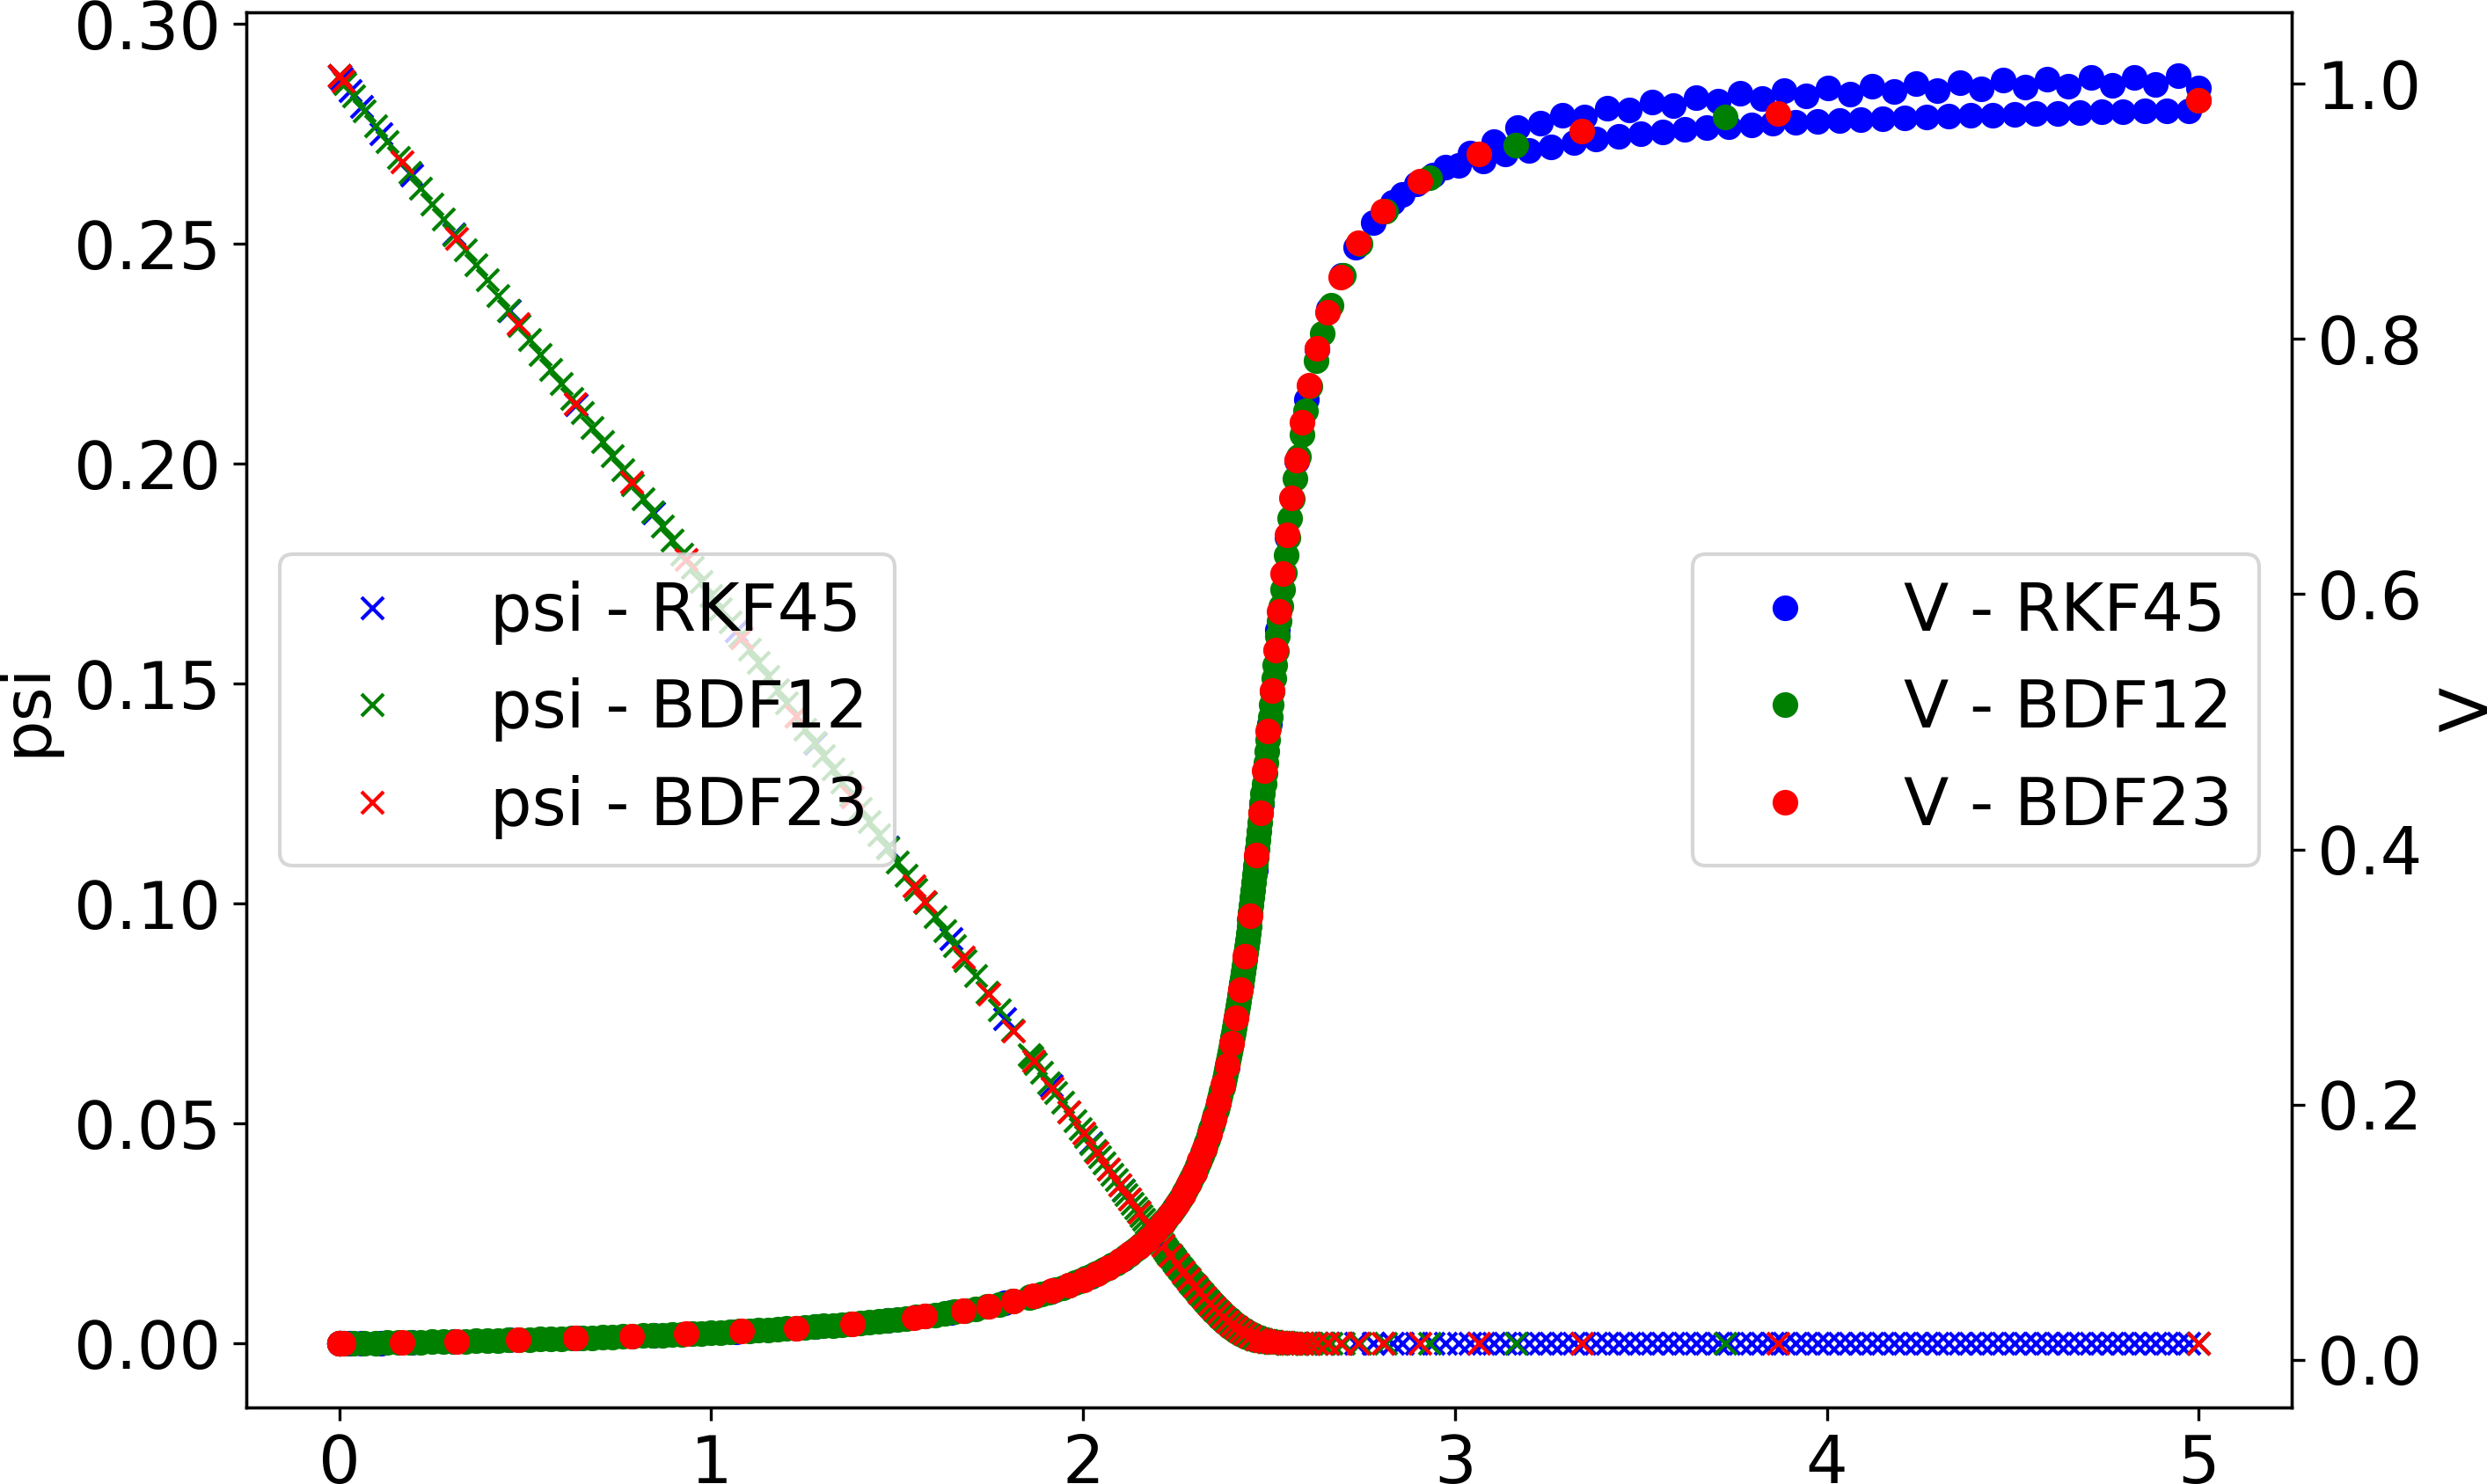
\includegraphics[width=1\textwidth]{images/timeEvolutionValues.png}
       	\subcaption{Evolution of the velocity $V$ and of the state variable $\psi$} 
        \label{fig:timeEvolutionValues}
    \end{subfigure}
    \begin{subfigure}{0.43\textwidth}
    	\centering
    	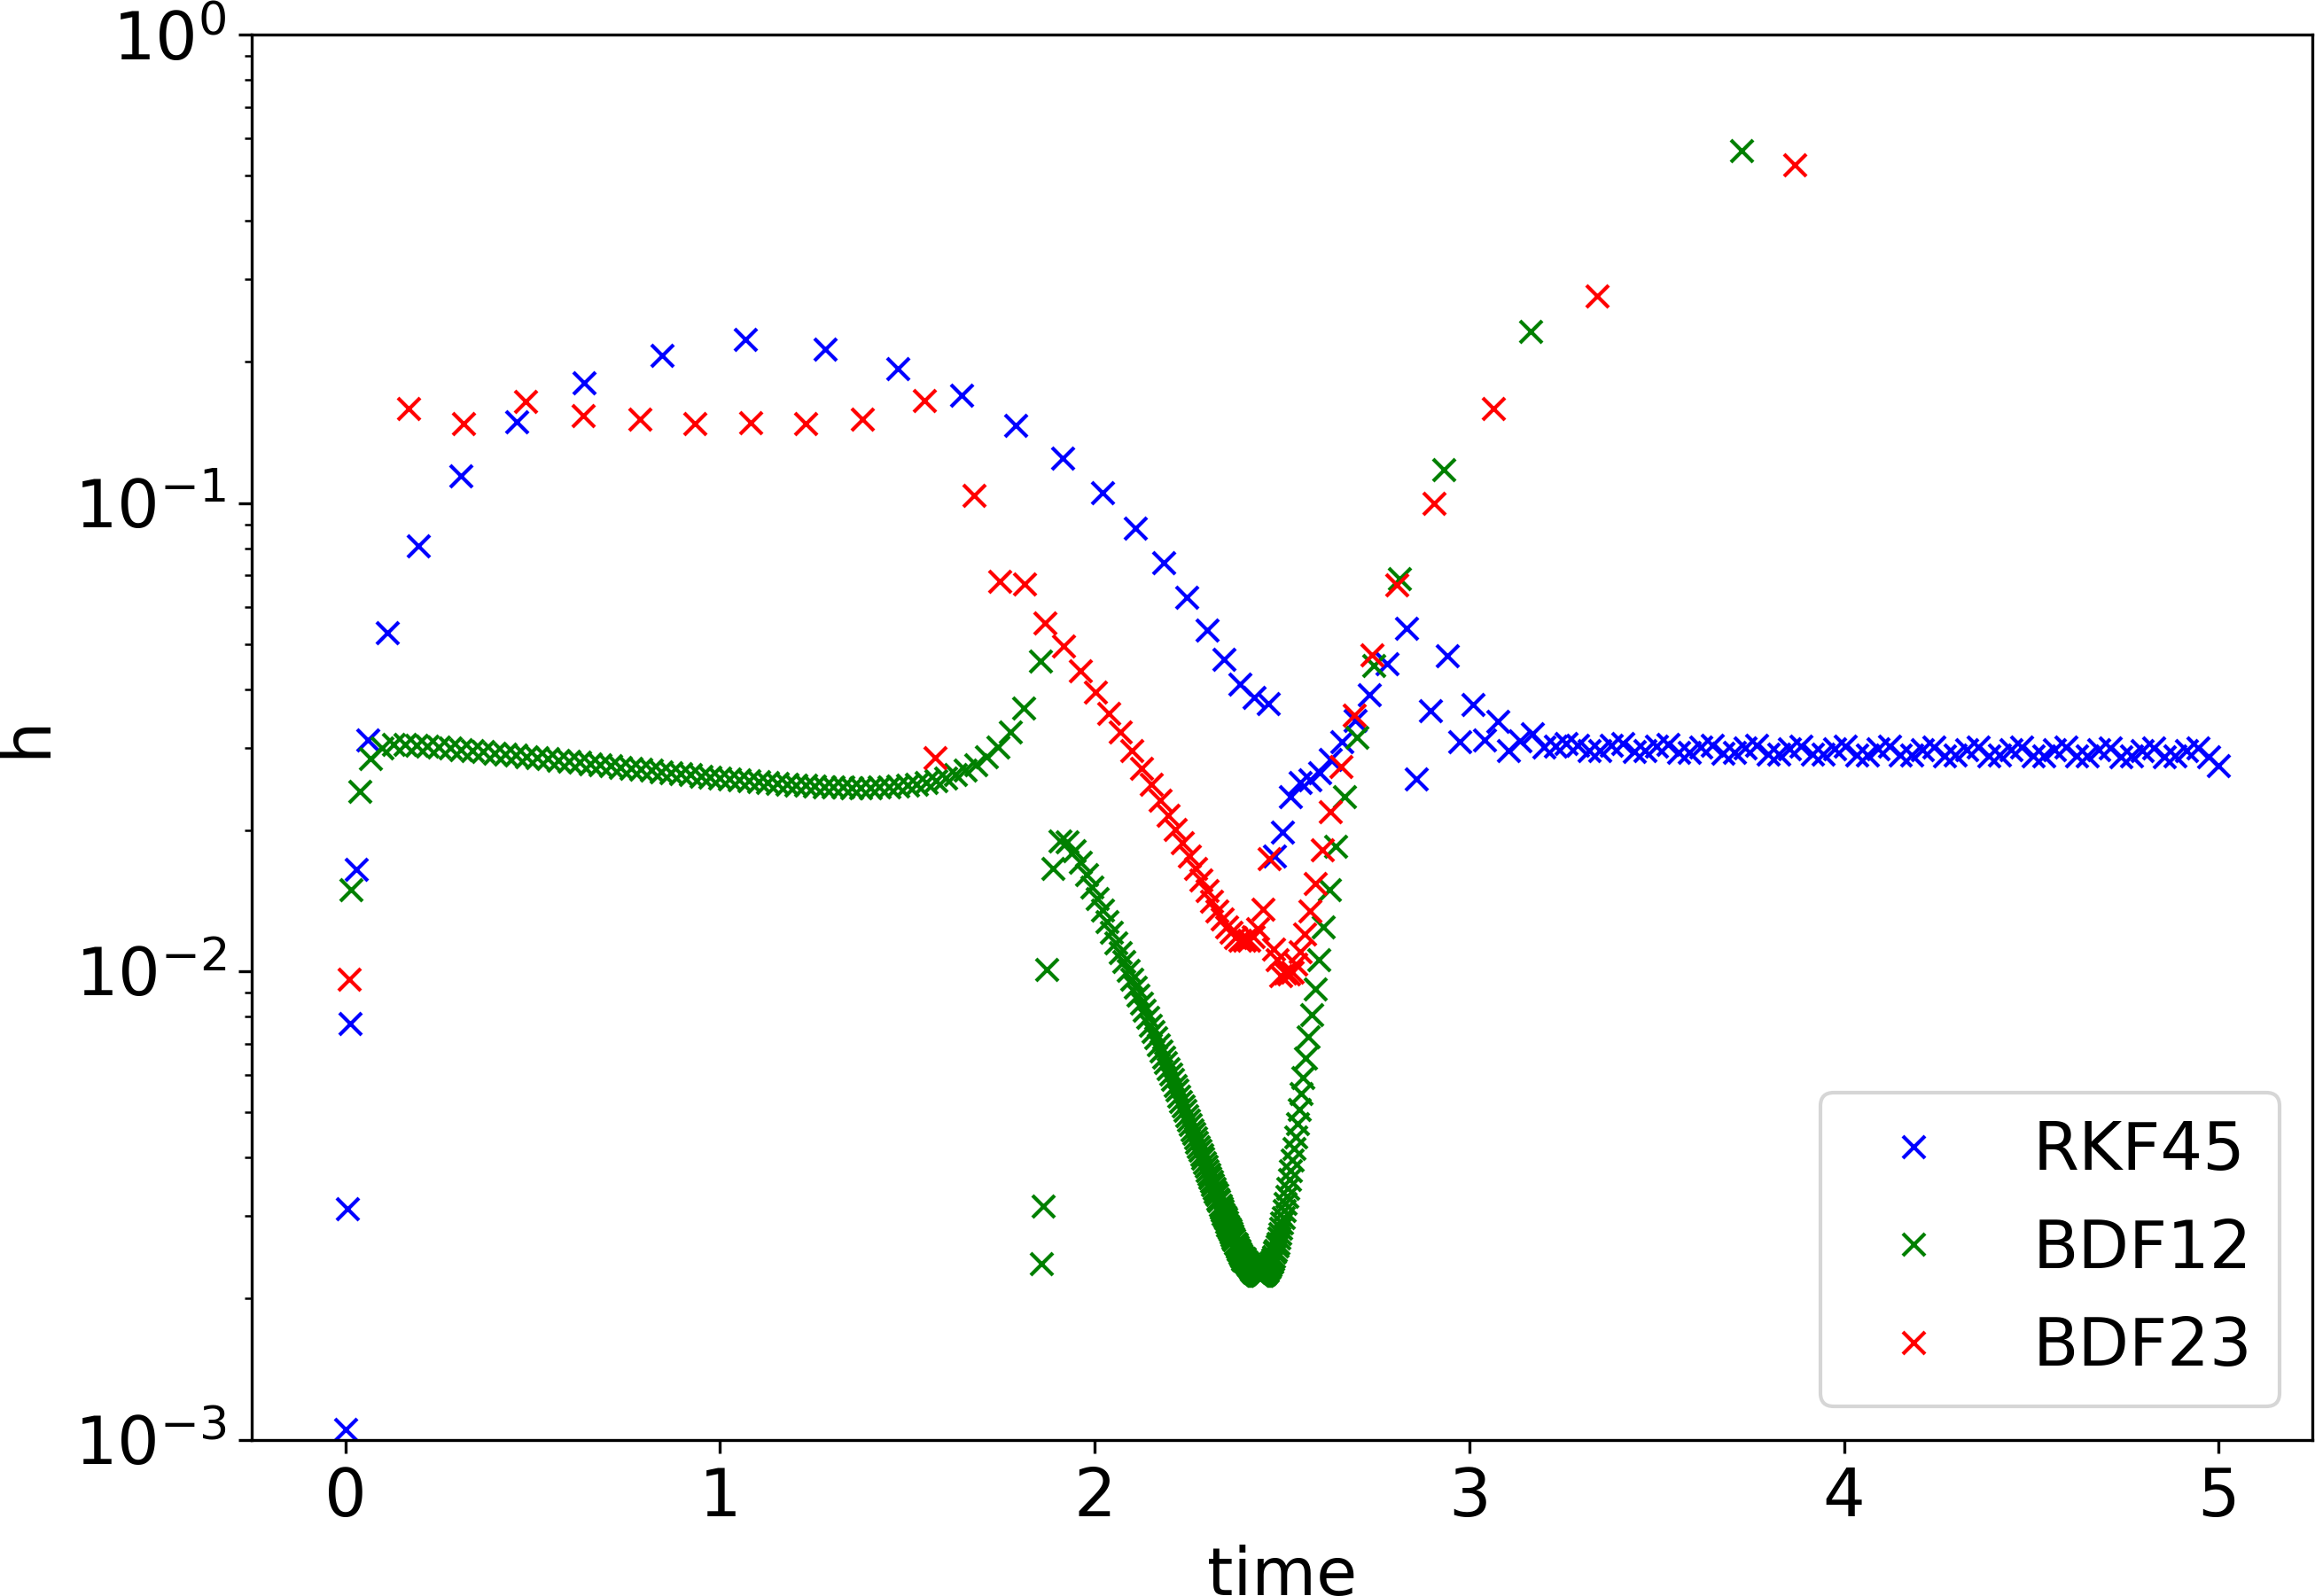
\includegraphics[width=1\textwidth]{images/timeEvolutionDT.png}
       	\subcaption{Evolution of the timestep size $h_n$} 
        \label{fig:timeEvolutionDT}
    \end{subfigure}
    \caption{Evolution of the solution and the timestep sizes of the single state problem defined in \autoref{eq:first_DAE_algeb} with the implemented numerical schemes}
\end{figure}

Now, the accuracy of the three numerical methods is compared. Therefore, \autoref{fig:timeEvolutionErrorPSI} depicts the evolution of the absolute difference between the numerical solution and the analytical solution of the state variable $\psi$. It is of interest to compare this error with the absolute error in velocity, shown in \autoref{fig:timeEvolutionVerror}. \\ 
As $\psi$ decreases, the error in $\psi$ increases steadily for all three numerical solvers. The implicit BDF methods produce two peaks in the evolution of the error, the first shortly before the end of the decrease and the second at the stiff transition of the velocity from 0 to 1. The norm of the error is much higher for BDF12 than for BDF23, despite the lower number of timesteps of the latter. The explicit RKF45 method produces a similar error norm as BDF12, but only in one peak at the beginning of the transition phase. In the end of the simulation, when $\psi$ stays around 0, all solvers match closely with the analytical solution and the error remains very low. On the other hand, the error in the velocity is very low for all solvers at the beginning and a peak in the error appears at the transition from 0 to 1. As usual, the highest error here appears for BDF12. Between the two remaining methods, RKF45 has the lowest error, which is astonishing for an explicit method applied to a stiff problem, especially considering the fact that in this section of the simulations, it also allows larger timesteps. Towards the end of the simulation, the error in velocity obtained by the two implicit methods vanishes again, however RKF45 produces suddenly very high errors which alternate between three different values. In \autoref{fig:timeEvolutionValues}, it can be seen that the velocity oscillates around the expected solution without getting closer to it. \\
It is important to realise that the error in $\psi$ and in the velocity are not directly correlated, thus a small error in $\psi$ does not necessarily lead to a small error in the velocity. It might thus be wise to reconsider the way the timestep size is controlled. So far, it only depends on the ratio between the local truncation error and a predefined tolerance value. This error is estimated by applying another numerical scheme with higher order, by taking the difference in $\psi$ of the two solutions as error estimate. Therefore, the velocity is not involved in the step size controller and the controller cannot ensure that the chosen timestep size guarantees sufficiently accurate results for the velocity. To ensure correct physical results, the controller needs to be extended in a way to restrict the timestep size with respect to some error estimate of the velocity. 

\begin{figure}[H]
    \centering
    \begin{subfigure}{0.43\textwidth}
    	\centering
    	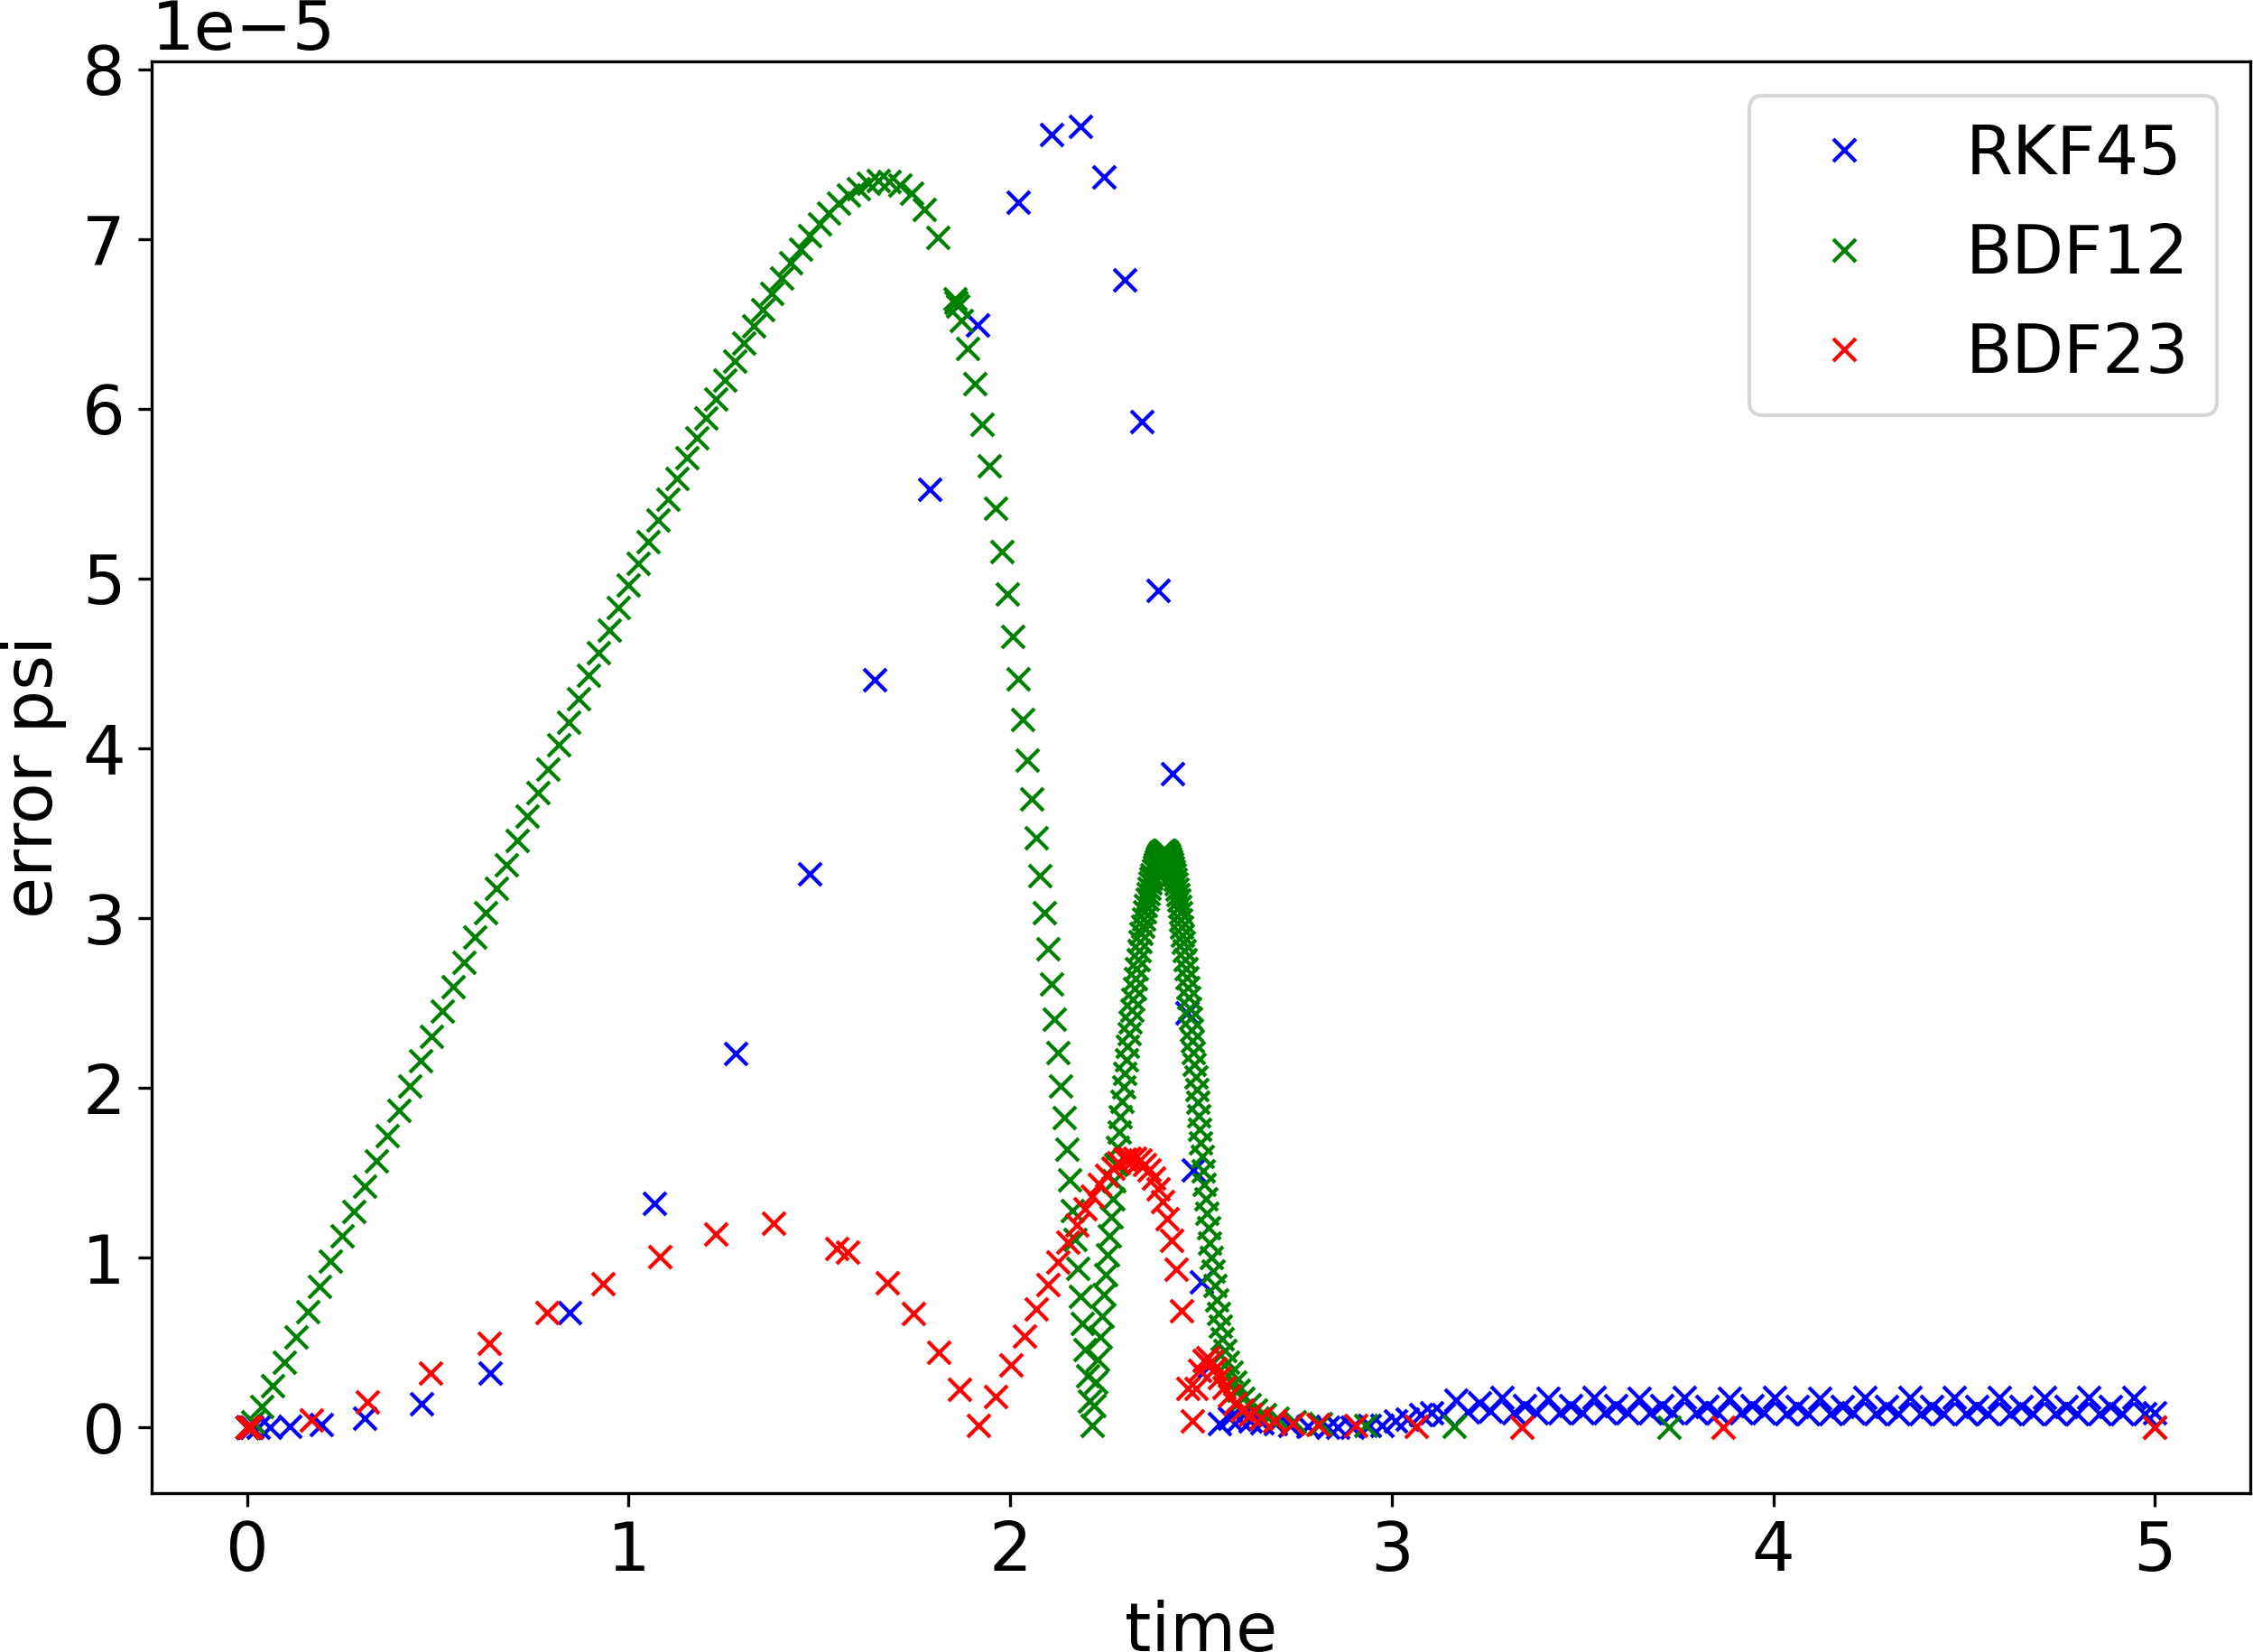
\includegraphics[width=1\textwidth]{images/timeEvolutionPSIerror.png}
       	\subcaption{Evolution of the absolute error of the state variable $\psi$} 
        \label{fig:timeEvolutionErrorPSI}
    \end{subfigure}
    \begin{subfigure}{0.43\textwidth}
    	\centering
    	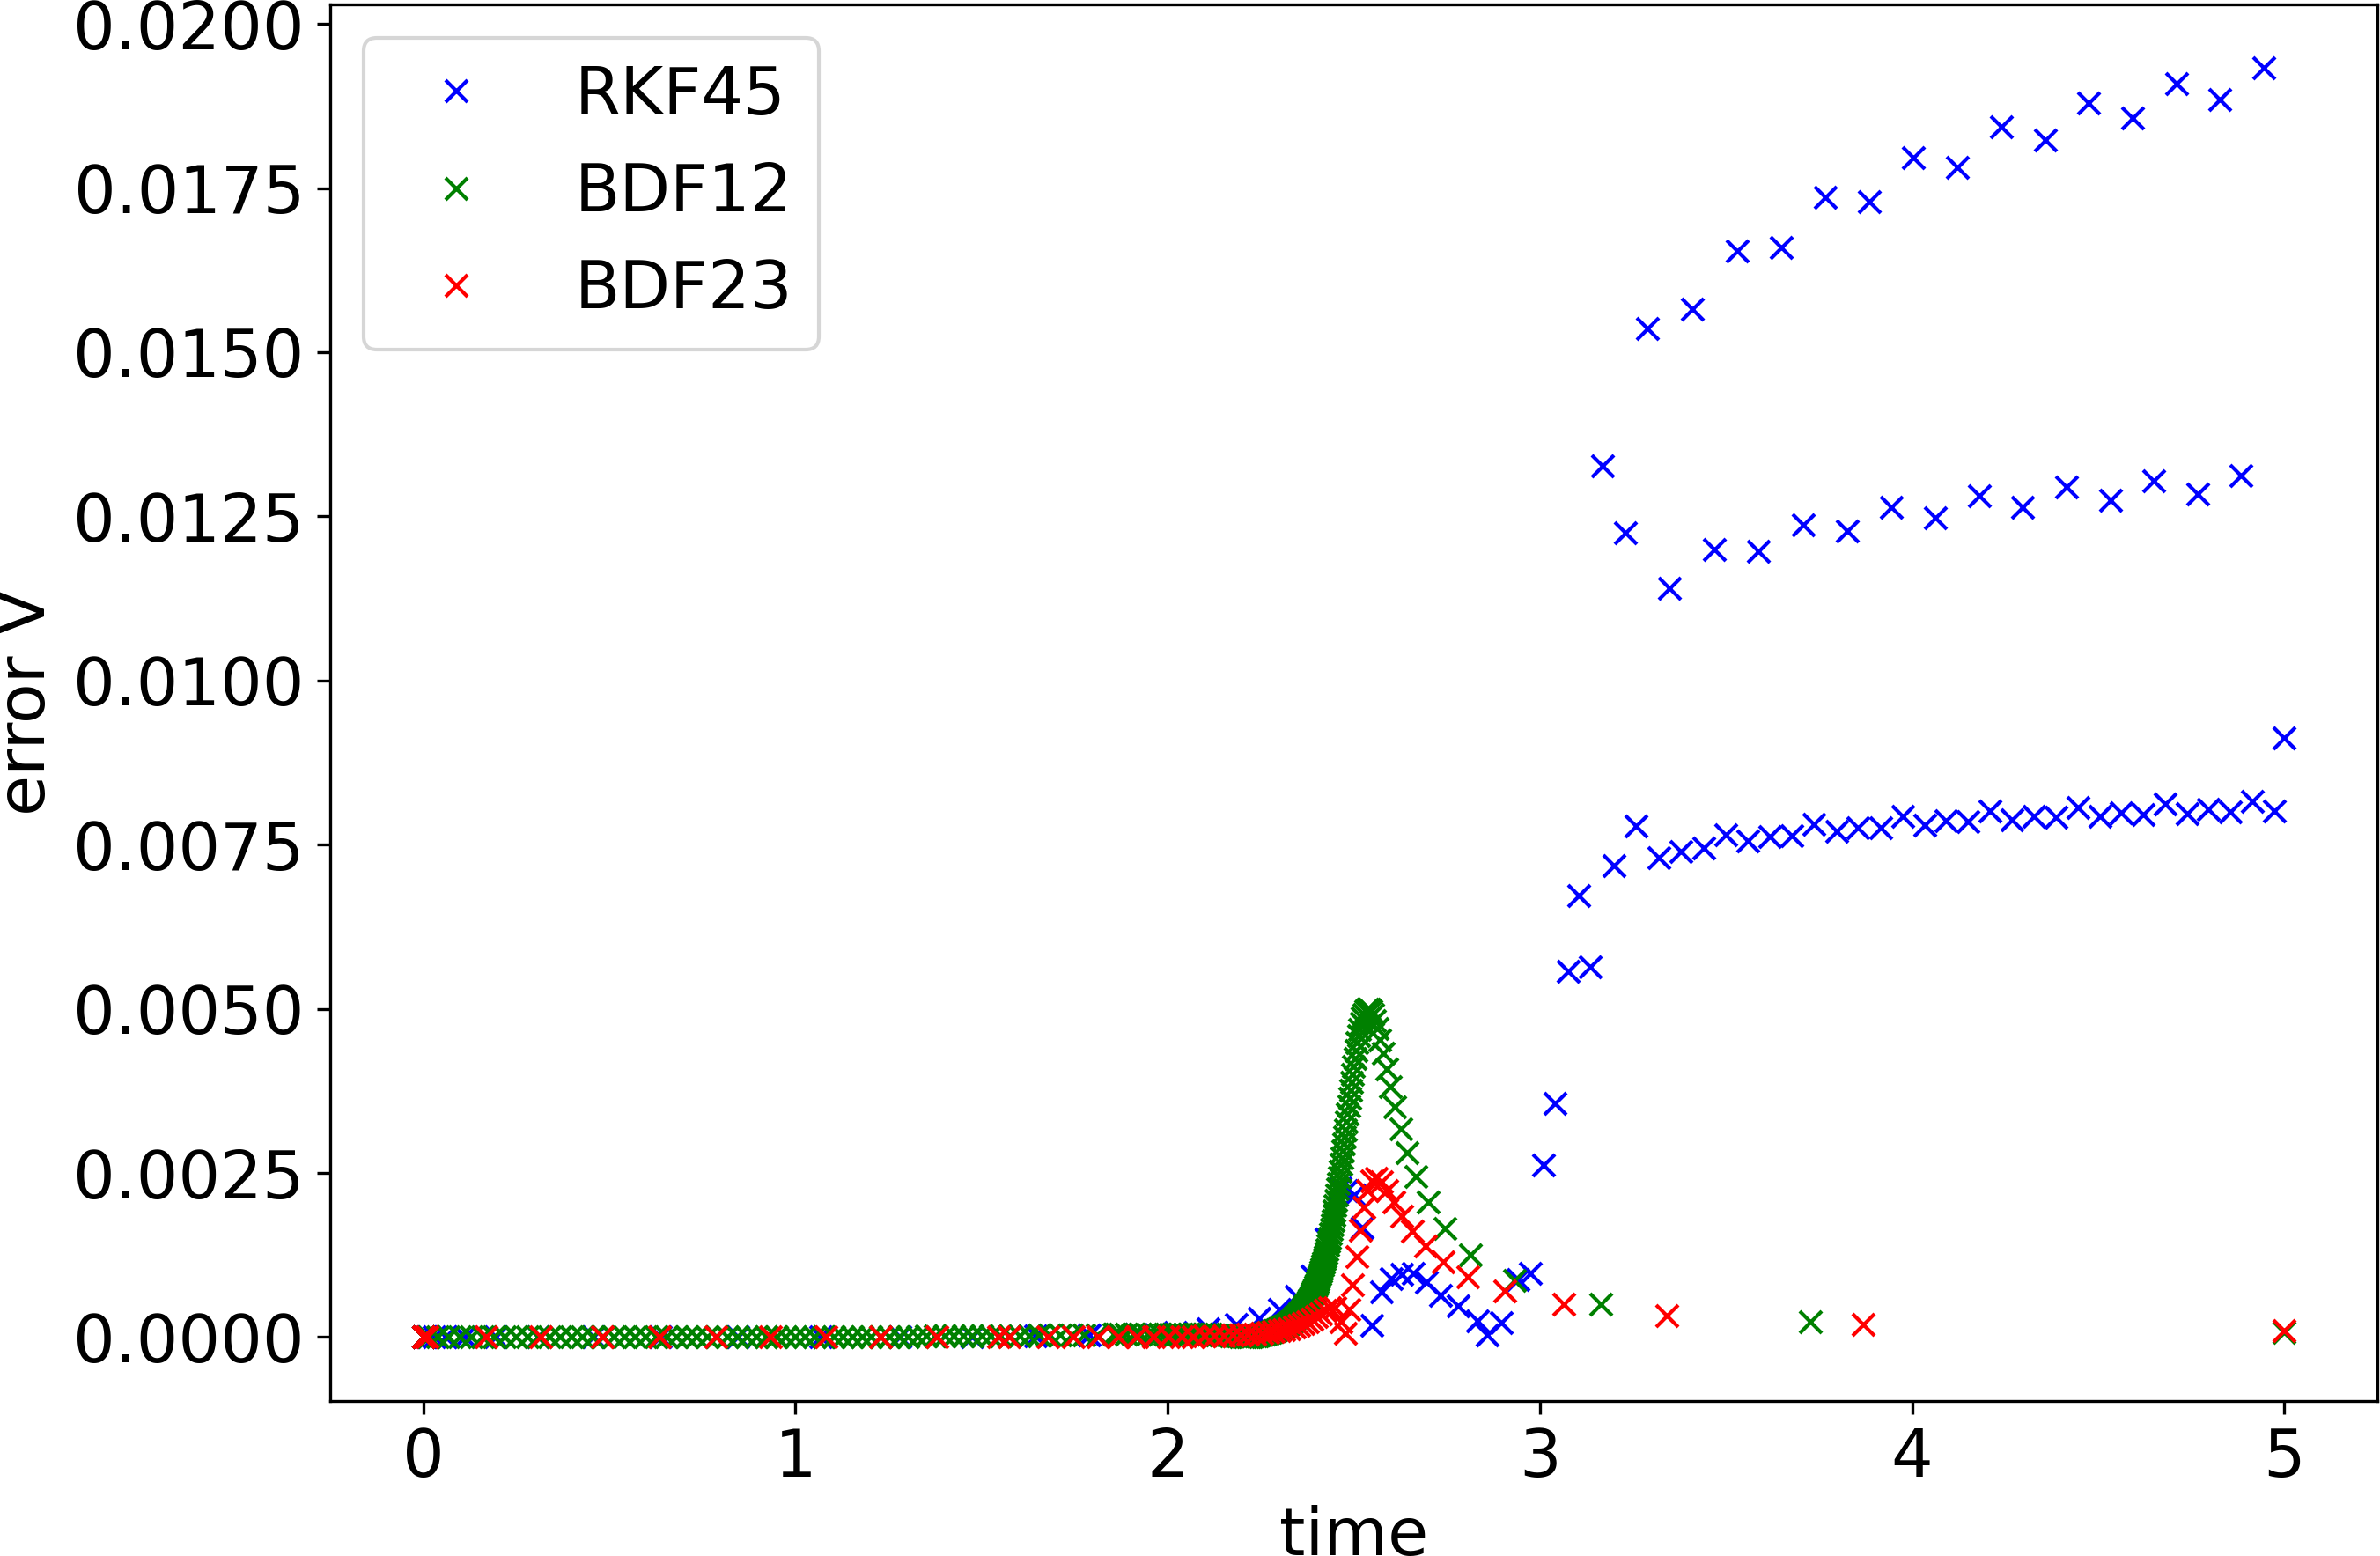
\includegraphics[width=1\textwidth]{images/timeEvolutionVerror.png}
       	\subcaption{Evolution of the absolute error of the velocity $V$} 
        \label{fig:timeEvolutionVerror}
    \end{subfigure}
    \caption{Evolution of the error for the single state problem defined in \autoref{eq:first_DAE_algeb} with the implemented numerical schemes}
\end{figure}

The whole theory of PI controller bases on an accurate error estimate, which is obtained in our case by calculating the solution with a higher order method. It is interesting to analyze whether the error estimate calculated in this way matches with the actual error to the analytical solution. The absolute error cannot be used as in the previous graphs, since the error estimate is calculated from the lower-order solution at the previous timestep. On the other hand, the local truncation error, which measures by how much the total error increases at each timestep, is much better suited to evaluate the accuracy of the error estimate. \\
In \autoref{fig:errorEstimateEvolutionALL}, the difference between the two solutions calculated at each timestep by any of the schemes, being the error estimate, plotted against the real local truncation error. In the initial phase, the two implicit methods estimate the error very closely to its real value. Even though the BDF12 method approximates it better than the BDF23 method, the high amount of executed timesteps in this phase accumulate the total error which turns out to be much worse. The estimate of the explicit RKF45 method roughly follows the real evolution of the local truncation error, but underestimates it by a large factor up to 5. During the transition phase, the situation is reversed, because the implicit methods fail at estimating correctly peaks in the evolution of the real error and remain instead around a same value. On the other hand, the RKF45 follows much better the evolution of the local truncation error, which explains its good performance in the transition phase with respect to the allowed timestep size and to the total error. In the final phase, the two implicit methods match again with the expected error values and the RKF45 method seems to fit exactly the real error, but it shows nonphysical oscillations which seem to correspond to the larges oscillations in the total error of the velocity. \\
Overall, the implicit methods yield the better error estimates except for the stiff transition which seems to be better handled by the explicit scheme. 

\begin{figure}[H]
    \centering
    \begin{subfigure}{0.32\textwidth}
    	\centering
    	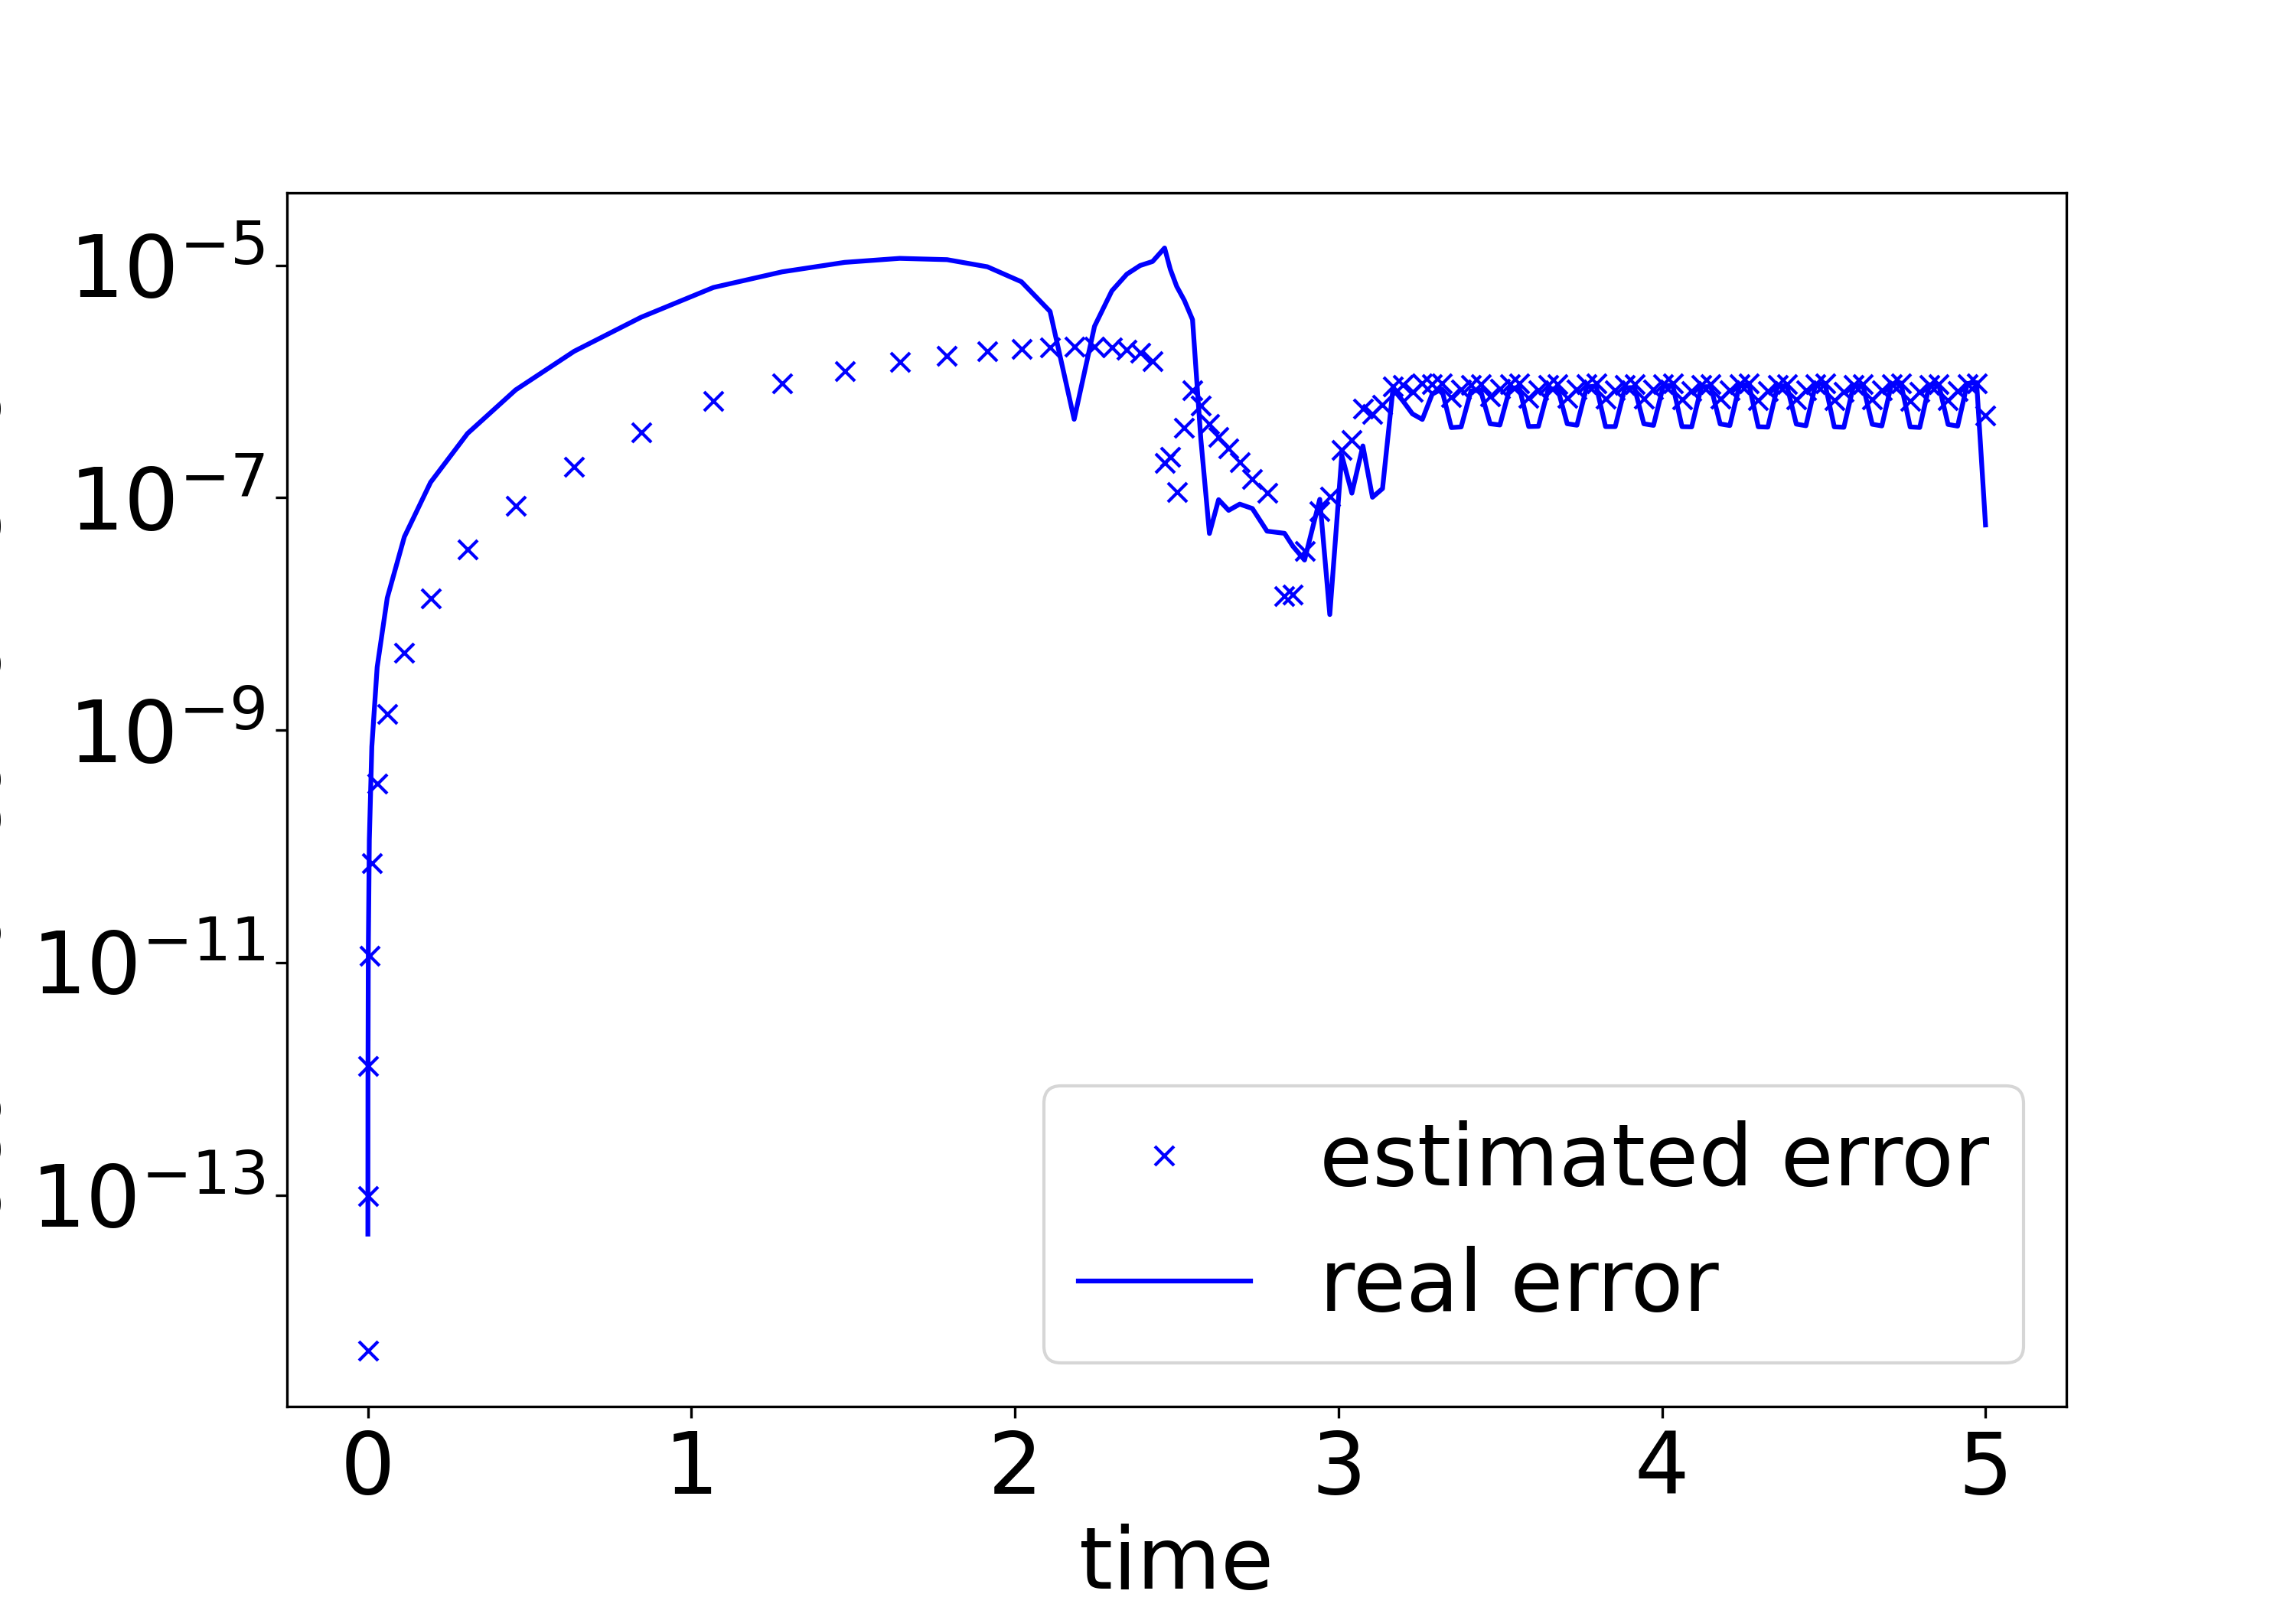
\includegraphics[width=1\textwidth]{images/errorEstimateRKF45.png}
       	\subcaption{\textbf{RKF45}} 
        \label{fig:errorEstimateEvolutionRKF45}
    \end{subfigure}
    \begin{subfigure}{0.32\textwidth}
    	\centering
    	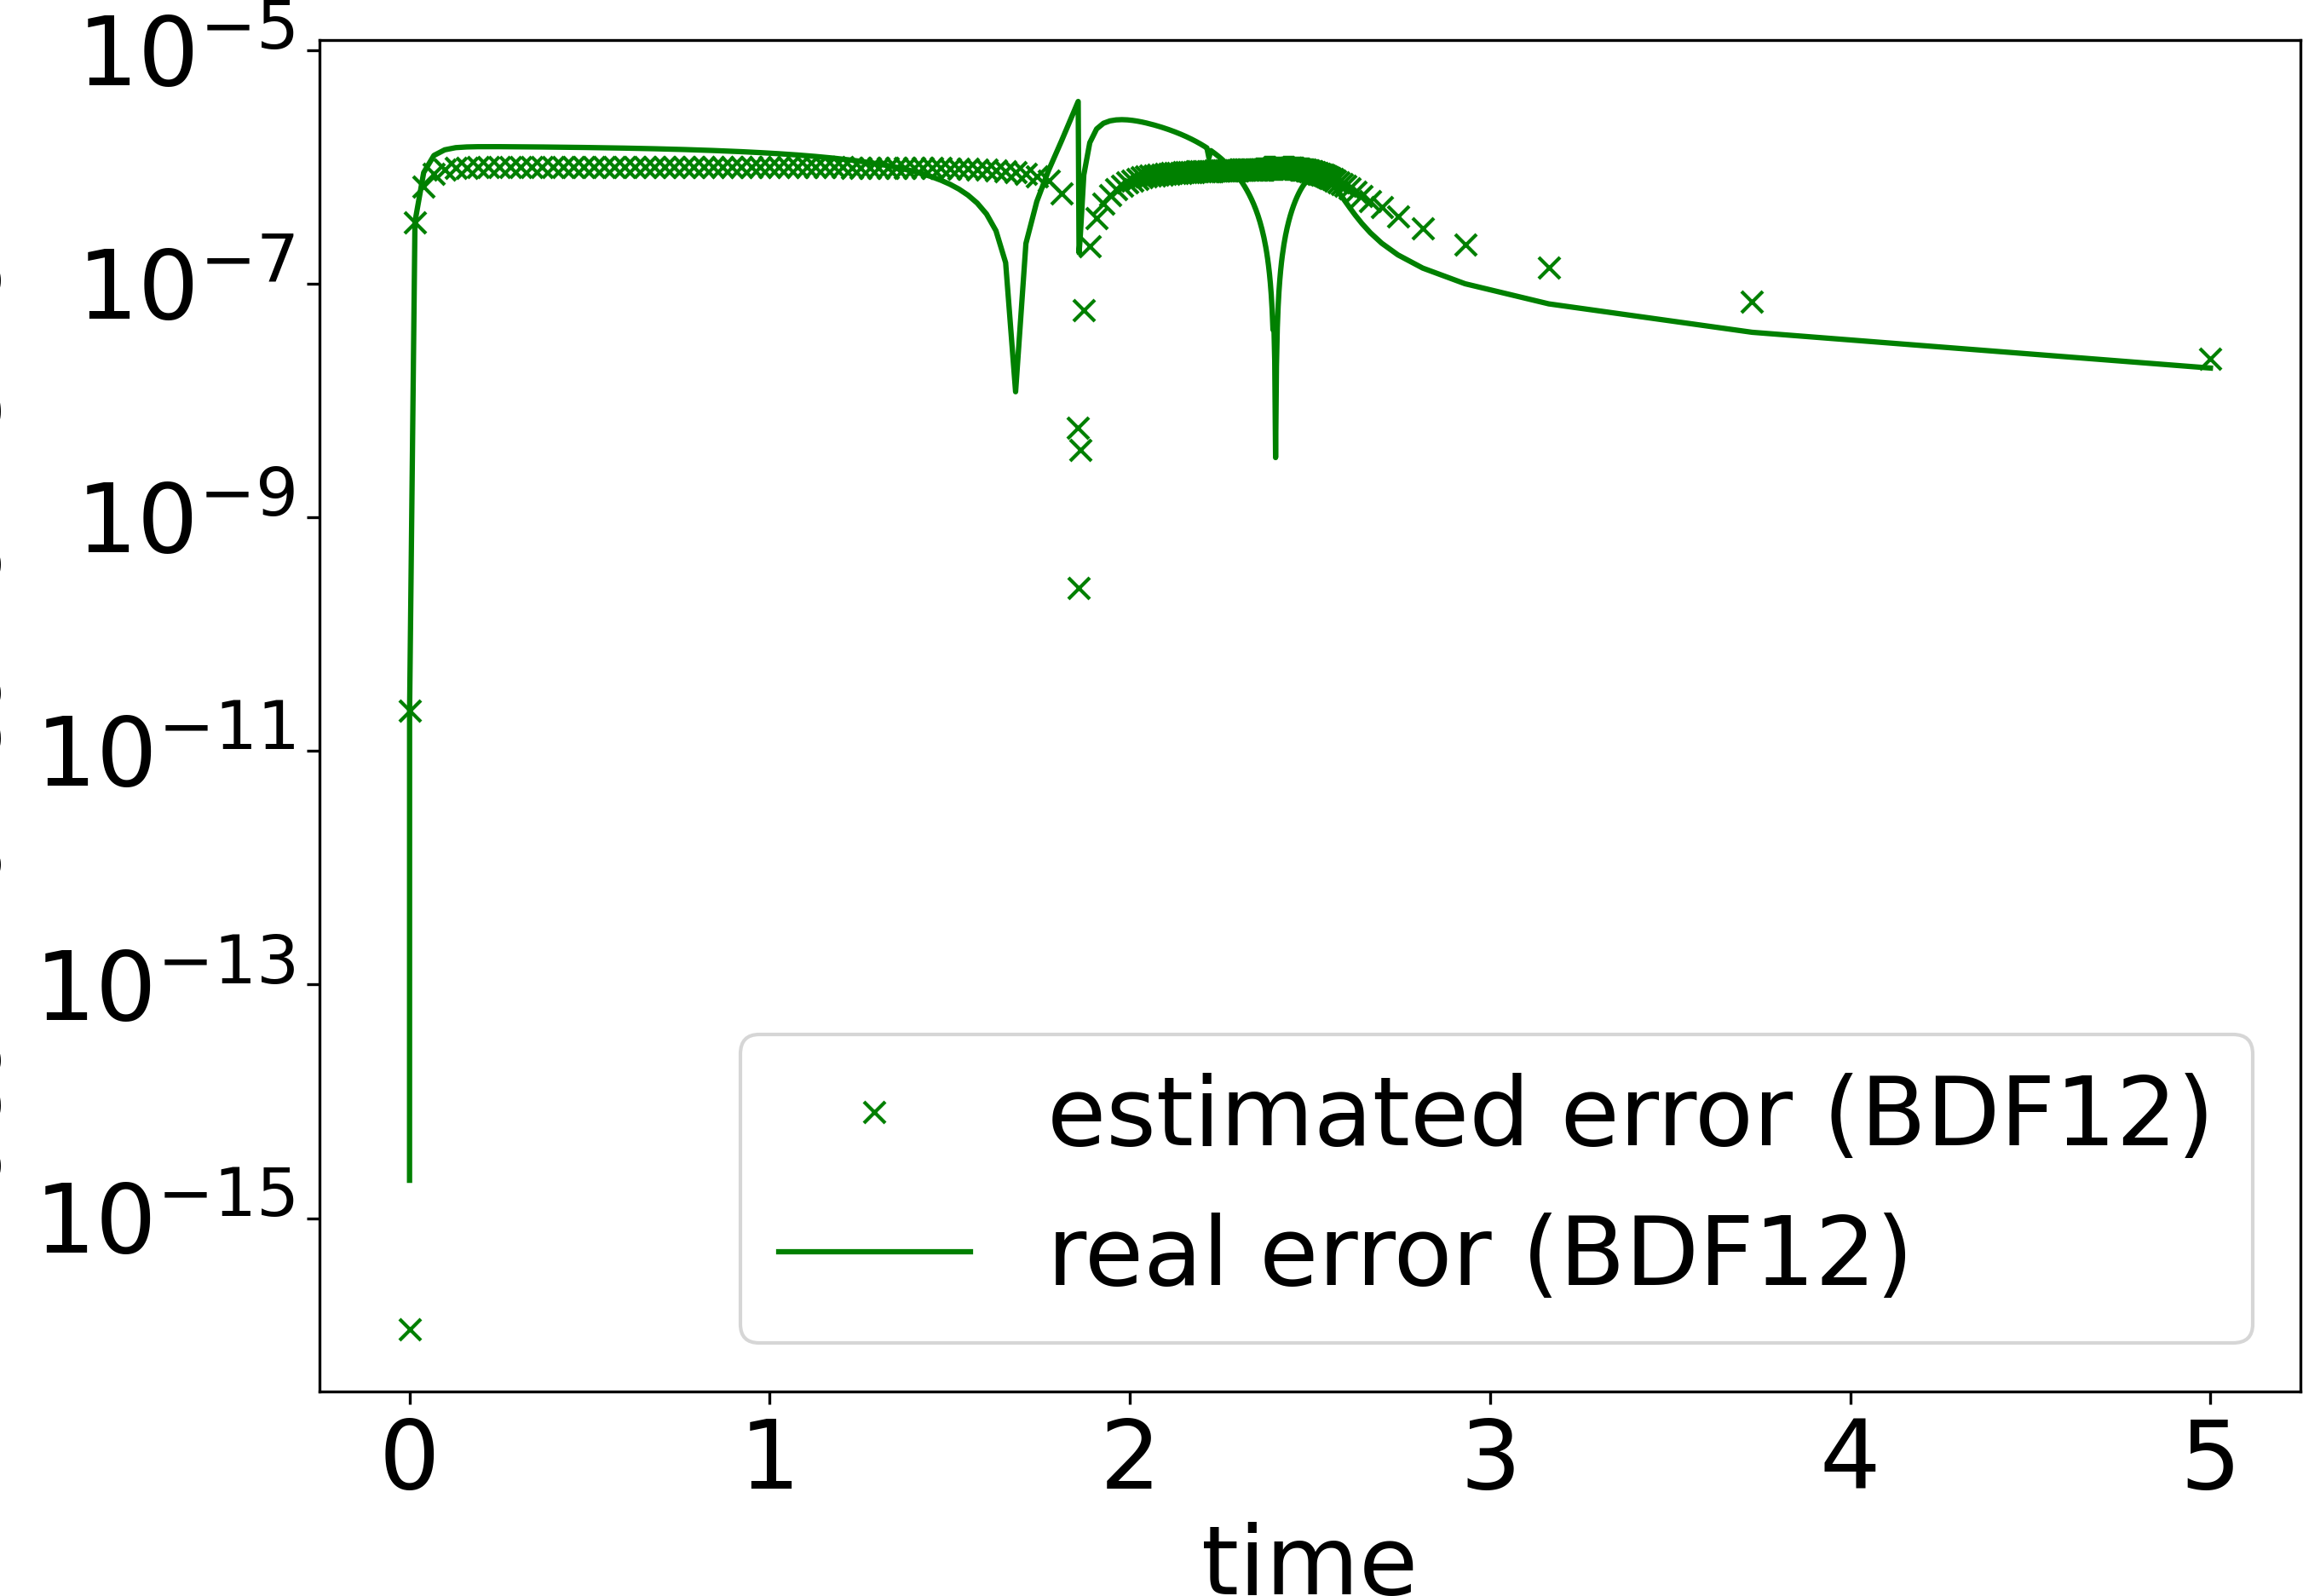
\includegraphics[width=1\textwidth]{images/errorEstimateBDF12.png}
       	\subcaption{\textbf{BDF12}} 
        \label{fig:errorEstimateEvolutionBDF12}
    \end{subfigure}
    \begin{subfigure}{0.32\textwidth}
    	\centering
    	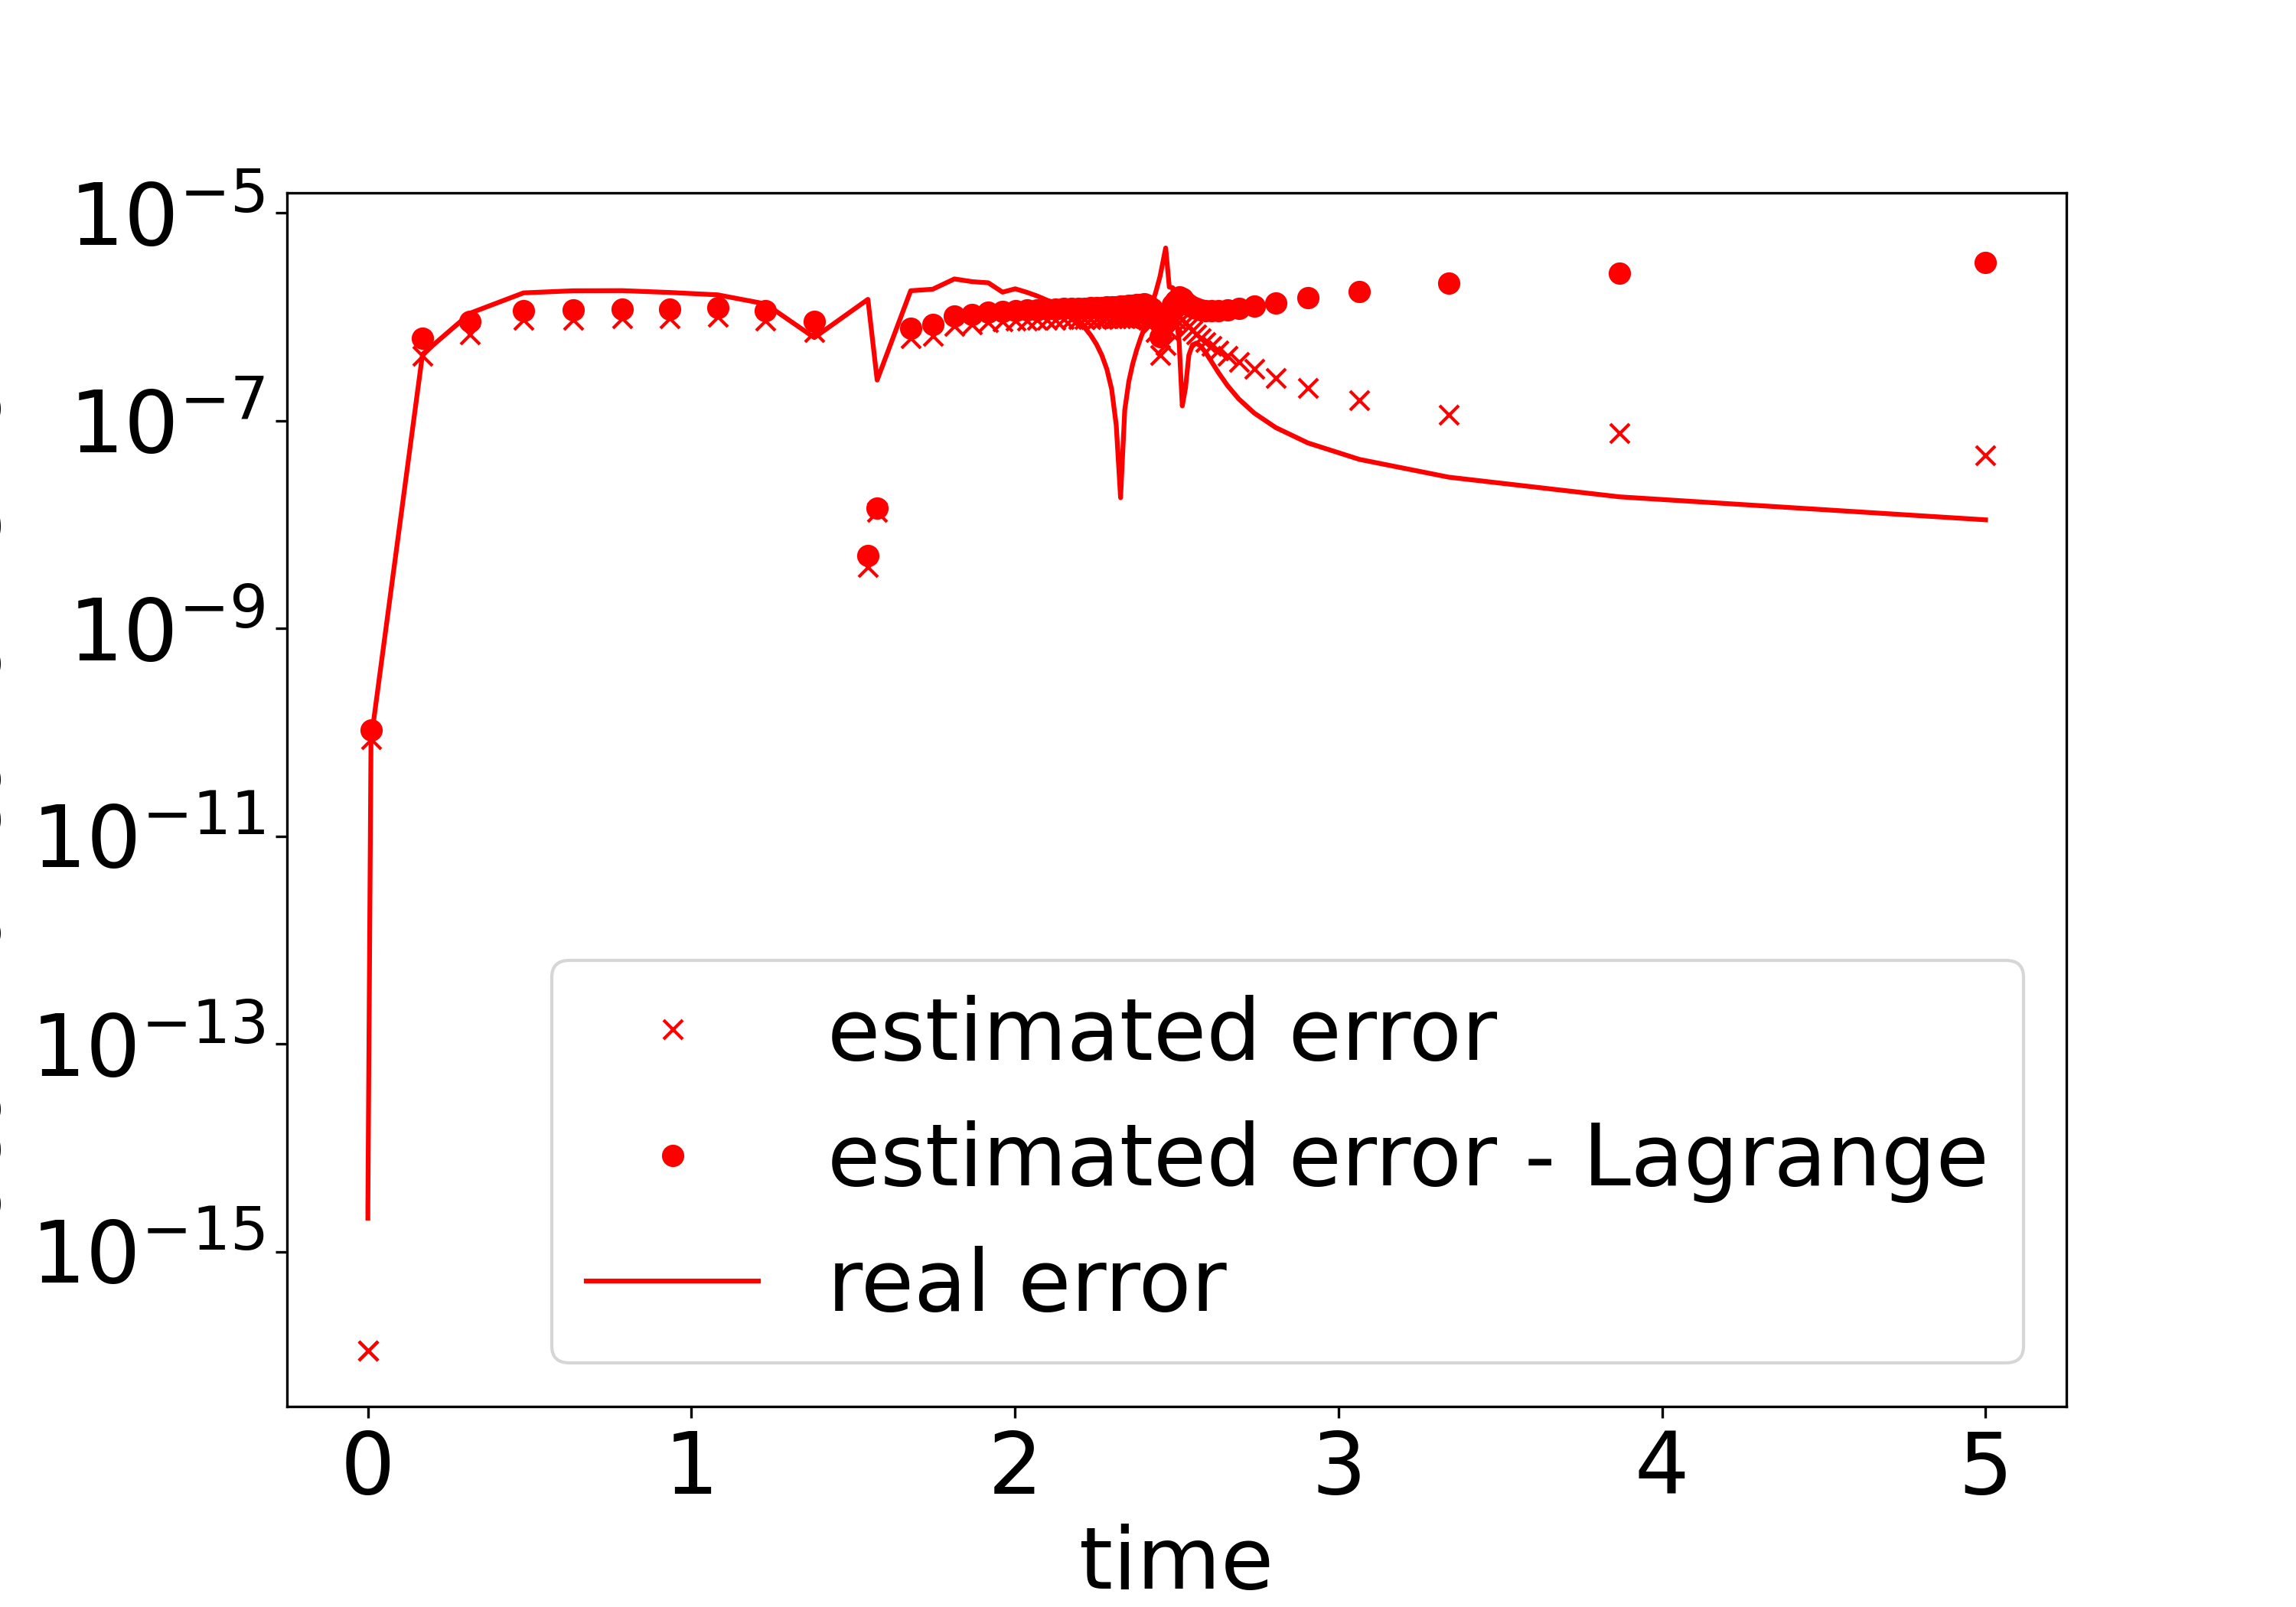
\includegraphics[width=1\textwidth]{images/errorEstimateBDF23.png}
       	\subcaption{\textbf{BDF23}} 
        \label{fig:errorEstimateEvolutionBDF23}
    \end{subfigure}
    \caption{Evolution of the local truncation error and of the error estimate for the single state problem defined in \autoref{eq:first_DAE_algeb} with the implemented numerical schemes}
    \label{fig:errorEstimateEvolutionALL}
\end{figure}

In conclusion, the implicit BDF23 method gives the best results because overall, the induced total error remains low, it allows for the highest timestep sizes and the local truncation error is generally well estimated. In contrast, the BDF12 method is restricted to much smaller timesteps which makes it unattractive for most simulations. Another negative side effect of the small timesteps is the large difference to the analytical solution since the local errors accumulate steadily. The explicit RKF45 fails if the velocity is too high, so it should not be used in such cases. However, it has a strong potential against the BDF23 method for very small velocities because it allows for larger timesteps and in the transition phase from low to high velocities because of the better estimate of the local truncation error.


%\section{Towards a More Physical Model}
%\subsection{Sliding block problem}
%The first considered problem is rather of theoretical nature than of practical relevance with the goal of seismic simulations. A more realistic model with a single variable could be the sliding block problem, in which a block, considered as a point mass, is attached to a spring which moves with constant velocity $V_0$ on a flat surface. The setup is shown in \autoref{fig:sliding_block_graph}. We are interested in the displacement $X$ of the center of mass of the block. The friction between the block and the surface is described by the non-linear law. 
%\begin{figure}[H]
%    \centering
%    \begin{tikzpicture}[scale=2] 
%        \draw[color=black, thick]
%        (1,0) to [short] (5,0){} 
%        (1.2,0.6) to [R,l=$k$,o-](2.8,0.6)
%        to node[short]{}(3,0.6)
%        (3,1.15) to node[short]{}(3,0.05)
%        (3,0.05) to node[short]{}(4.5,0.05)
%        (4.5,0.05) to node[short]{}(4.5,1.15)
%        (3,1.15) to node[short]{}(4.5,1.15)
%        (3.75,0.6) node[]{\large{\textbf{M}}}
%        (1.2,0.8) node[]{$V_0$}
%        ;
%        \draw[<-,color=black, thick] (1.05,0.7) to node[short]{}(1.35,0.7);
%    \end{tikzpicture}
%    \caption{Sliding block problem}
%    \label{fig:sliding_block_graph}
%\end{figure}

\chapter{Two-Dimensional SEAS model}
In a second step we consider a trivial SEAS model with only two dimensions and square, symmetric tectonic plates.

\section{Physical Description}
\label{ssec:physicalDescriptionSEAS2D}
--- write down Poisson/elasticity equation for the domain --- \\
--- rate and state laws for the fault --- \\
describe what all variables mean and stuff...
Ageing law: 
\begin{equation}
    \dot{\psi} = g(\psi, V) = \frac{bV_0}{L}e^{\frac{f_0 - \psi}{b}} - \frac{V}{V_0}
\end{equation}
Friction law: 
\begin{equation}
    0 = \tau(U) - a\sigma_n(U) \text{arsinh}\left(\frac{V}{2V_0}e^{\frac{\psi}{a}}\right) - \eta V
\end{equation}


\section{BP1 problem}
--- read more about BP1 and find good citations --- \\
The displacement is applied orthogonal to the represented plane, thus, if the mesh is located in the X-Y plane, each element has one traction, velocity and displacement component acting in the Z direction. In this model problem, the represented tectonic plates have a symmetric layout and move in opposite direction, as one moves into the plane and the other one out of the plane. Therefore, it is enough to consider only one half of the domain, as the results in the other half will be identical, but with opposite sign. \autoref{fig:mesh_BP1_200_fault_elements} depicts the half-domain on which the solution is calculated. The fault here is located on the left side of the domain.
\begin{figure}[H]
    \centering
    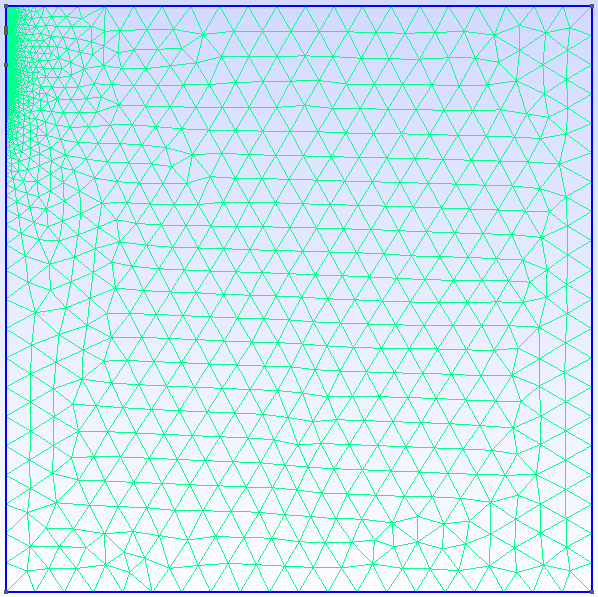
\includegraphics[width=0.4\textwidth]{images/BP1_MESH_200.png}
    \caption{Space discretization of the BP1 problem with 200 elements on the fault}
    \label{fig:mesh_BP1_200_fault_elements}
\end{figure}

In the considered example, we choose the mesh such that there are 200 elements at the fault. The lower end of the plates is pulled with a constant velocity $V_0 = 10^{-6} m\cdot s^{-1}$. 

\section{Formulation of the Discontinous Galerkin}

--- write something about DG --- \\ 


The numerical integration is achieved with the Gaussian quadrature. For that, Gauss-Legendre polynomials up to order $p$ are chosen to interpolate relevant values on each element. Dependent on the chosen order $p$, the solution has to be calculated at different points $x_i$ within the element and, associated with the correct weights to interpolate the data over the entire element, the integration is exact with respect to the interpolation polynomials. \\
--- write more about GQ --- \\

To solve the Poisson equation, it is necessary to evaluate the integral over the entire element and to handle boundary conditions and the fault, the integral over the edges of the element is needed. 


\section{Formulation of the DAE}
The problem stated in \autoref{ssec:physicalDescriptionSEAS2D} can be written in the form of a DAE:
\begin{align}
    \dot{S_i} &= V_i \label{eq:SEASDAE_dV_dt} \\
	\dot{\psi_i} &= g(\psi_i, V_i) =\frac{bV_0}{L}\left(e^{\frac{f_0-\psi_i}{b}} - \frac{V_i}{V_0}\right) \label{eq:SEAS_DAE_ageing_law} \\
	0 &= f_i(U,\psi,V) = \tau_i(U) - a\sigma_n\text{arsinh}\left(\frac{V_i}{2V_0}e^{\frac{\psi_i}{a}}\right) -\eta V_i \label{eq:SEASDAE_frictionLaw}\\
    0 &= AU - b(S) \label{eq:SEAS_DAE_AU=b}  
\end{align}
The index $i$ refers to all interpolation points of the elements located on the fault, meaning that $S_i$, $V_i$ and $\psi_i$ are respectively the displacement, the velocity and the value of the state variable on the fault. In the two-dimensional case, the displacement $S_i$ at the fault is related to $U_i$ by $\llbracket U_i \rrbracket = U_i^+ - U_i^- = -S_i$. The displacements $U_i^+$ and $U_i^-$ correspond to the displacements on the two sides of the fault, for the current symmetric problem, they have the same magnitude with opposite signs.\\
 

\subsection{Formulation as an ODE}
The first approach to solve the problem is to formulate the system as a classical ODE. The solution vector contains the values for the slip and for the state variable, and at each timestep, the the slip rate $V$ is calculated from \autoref{eq:SEASDAE_frictionLaw} from the state with an iterative solver.
\begin{align}
	\label{eq:ODE_formulation_SEAS}
	x &= \begin{pmatrix}
		S \\ \psi
	\end{pmatrix} & \dot{x} &= \begin{pmatrix}
								  \dot{S} \\ \dot{\psi}
							   \end{pmatrix} = \begin{pmatrix}
												   V(S,\psi) \\ g(\psi, V)
											   \end{pmatrix} = F
\end{align} 
Such a formulation allows us to use many well-known and proved numerical schemes, both implicit and explicit. 

\subsection{Formulation as DAE}
The ODE form looks pretty and like an easy-to-tackle numerical problem, but may run into some trouble because of the implicit evaluation of the slip rate. For example, one major encountered problem is the impossibility to construct an analytic expression of the Jacobian matrix, detailed in \autoref{sssec:Jacobian_ODE}, which makes the ODE formulation of the problem less suitable for implicit numerical schemes. Alternatively, the friction law could be solved for the slip rate together with the time-variant solution components. The solution vector is then extended by one quantity, and the evaluation of the slip rate with a separate iterative does not occur anymore.
\begin{align}
	\label{eq:DAE_formulation_SEAS}
	x &= \begin{pmatrix}
			S \\ \psi \\ V
		 \end{pmatrix} & \dot{x} &= \begin{pmatrix}
										\dot{S} \\ \dot{\psi} \\ 0
									\end{pmatrix} = \begin{pmatrix}
										V \\ g(\psi, V) \\ f(S,\psi,V)
									\end{pmatrix} = F
\end{align}
This system cannot be used anymore with pure explicit solvers, since no time discretization can be set up for the algebraic equation. It is however well-suited for implicit methods, which iteratively solve for the time-variant quantities $S$ and $\psi$ as well for the algebraic state $V$. A notable advantage of this formulation is that the tolerances of the numerical solver can be specified independently for $S$, $\psi$ and $V$, whereas in the ODE formulation of the problem, the error control is limited to the parameters $S$ and $\psi$. 

\subsection{Compact formulation as a DAE}
The preceding form of the DAE cannot be used directly with the DAE interface, which allows to split the problem in to functions $F$ and $G$ that have to be equal, where, in addition to time, $F$ depends on the solution vector $x$ and its time derivative $\dot{x}$ and $G$ depends only on the solution vector $x$. 
\begin{align}
	F(t, x,\dot{x}) = G(t,x) 
\end{align}
In our case, the solution vector contains as in the ODE formulation the components of the slip $S$ and of the state variable $\psi$. It is important to remember that the slip rate is the time derivative of the slip, so the variables $\dot{S}$ and $V$ are equal and can be interchanged.
\begin{align}
	\label{eq:DAE_compact_formulation_SEAS}
	x &= \begin{pmatrix}
			S \\ \psi
	     \end{pmatrix} & F(t, x,\dot{x}) &= \begin{pmatrix}
												f(S,\psi,V) \\ \dot{\psi} - g(\psi, V)
											\end{pmatrix} = \begin{pmatrix}
																0 \\ 0
															\end{pmatrix} = G(t,x)
\end{align}
As in the developed DAE formulation, the friction law is solved along with time-variant quantities $S$ and $\psi$. It therefore requires an iterative solver method from an implicit time solver and is cannot be used in general only with an explicit integrator. \\
Another class of solvers, the so called IMEX (implicit-explicit) solvers [cite IMEX], offer an interesting approach to numerically solve this problem, by mixing an implicit, iterative method for the algebraic states with an explicit method for the remaining simple time-dependent quantities. Technically, the function $F()$ is expected to be integrated implicitly, while the right-hand side function $G()$ is solved explicitly. In the given formulation, the right hand side is equal to 0, this means that the system has to be solved fully implicitly and the advantages of IMEX methods cannot be used here. 

\section{Formulation of the Jacobian}
To use implicit time solvers, the Jacobian matrix of the right-hand side of the ODE in (\ref{eq:SEAS_DAE_ageing_law}) and (\ref{eq:SEASDAE_dV_dt}) has to be computed in the Newton iteration. In general, if it is unknown, it is approximated along with the solution during the Newton iteration using for instance a Broyden iteration [cite Broyden]. However, this impairs the convergence speed of the Newton iteration compared to the analytical expression. It is especially relevant if the explicit-implicit formulation of the problem is chosen, for which an iterative solver is indispensable. 

\subsection{Analytical Derivation of the Jacobian matrix}
\label{ssec:AnalyticalDerivationOfTheJacobianMatrix}
In a first step, we try to derive an analytical expression of the Jacobian for both the ODE and the DAE formulation of the problem.

\subsubsection{Jacobian of the ODE system}
\label{sssec:Jacobian_ODE}
For the ODE formulation in \autoref{eq:ODE_formulation_SEAS}, it is impossible to calculate an analytical expression of the Jacobian matrix. In the following, it will be shown, why any attempt to calculate it would fail. The Jacobian $\mathbf{J}_{\psi,S}(F)$ consists of four block matrices, which each contains the Jacobians related to the two quantities:
\begin{equation}
	\label{eq:Jacobian_ODE_formulation}
	\mathbf{J}_{\psi_h,S_j}\left(F_i\left(\psi,V(\psi,S)\right)\right) = \begin{pmatrix} 
	\frac{\partial V_i}{\partial S_j} &
	\frac{\partial V_i}{\partial \psi_j} \\ 
	\frac{\partial g(\psi_i,V_i)}{\partial S_j} &
	\frac{\partial g(\psi_i,V_i)}{\partial \psi_j}  \end{pmatrix}
\end{equation}
To calculate the partial derivatives of $V_i(\psi_i,S_i)$, we need to consider the friction law $f(U, \psi,V)$. For any chosen values for $\psi$ and $S$, V is evaluated in a way that $f(U(S), \psi, V(\psi,S))$ vanishes. Therefore, we can state that $df/d\psi = 0$ and $df/dS = 0$. With the expression of the total derivative, we obtain the following equations:
\begin{align}
	0 &= \frac{df_k}{dS_j} =     
	\frac{\partial f_k}{\partial S_i}\frac{d S_i}{d S_j} + 
	\frac{\partial f_k}{\partial V_i}\frac{d V_i}{d S_j} + 
	\frac{\partial f_k}{\partial \psi_i}\frac{d \psi_i}{d S_j} 
	\qquad\Leftrightarrow\qquad
	\frac{d V_i}{d S_j} = -\left(\frac{\partial f_k}{\partial V_i}\right)^{-1}\left(\frac{\partial f_k}{\partial S_l}\frac{d S_l}{d S_j} + \frac{\partial f_k}{\partial \psi_l}\frac{d \psi_l}{d S_j} \right) 
	\label{eq:SEASDAE_totaldV_dS} \\
	0 &= \frac{df_k}{d\psi_j} = 
	\frac{\partial f_k}{\partial \psi_i}\frac{d \psi_i}{d \psi_j} + 
	\frac{\partial f_k}{\partial V_i}\frac{d V_i}{d \psi_j} + 
	\frac{\partial f_k}{\partial S_i}\frac{d S_i}{d \psi_j}
	\qquad\Leftrightarrow\qquad
	\frac{d V_i}{d \psi_j} = -\left(\frac{\partial f_k}{\partial V_i}\right)^{-1}\left(\frac{\partial f_k}{\partial \psi_l}\frac{d \psi_l}{d \psi_j}  + 
	\frac{\partial f_k}{\partial S_l} \frac{d S_l}{d \psi_j}\right)
	\label{eq:SEASDAE_totaldV_dpsi}
\end{align}
It is allowed to take the inverse of the matrix $\frac{\partial f}{\partial V}$, whose expression is given in \autoref{eq:partial_df_dV} and is accordingly a diagonal matrix with non-zero entries. Further, the derivatives of the slip rate with respect to the state variable and the slip can also be reformulated with the formula of total derivatives: 
\begin{align}
\frac{dV_i}{dS_j} &= \frac{\partial V_i}{\partial S_k}\frac{d S_k}{d S_j} + \frac{\partial V_i}{\partial \psi_k}\frac{d\psi_k}{dS_j} &
\frac{dV_i}{d\psi_j} &= \frac{\partial V_i}{\partial \psi_k}\frac{d \psi_k}{d \psi_j} +  \frac{\partial V_i}{\partial S_k}\frac{dS_k}{d\psi_j} 
\end{align}
As such, the two upper block matrices in the full Jacobian from \autoref{eq:Jacobian_ODE_formulation} are obtained by solving the following linear system: 
\begin{equation}
\label{eq:systemJacobianSlipRate}
\begin{cases}
	\frac{\partial V_i}{\partial S_k}\frac{d S_k}{d S_j} + \frac{\partial V_i}{\partial \psi_k}\frac{d\psi_k}{dS_j} = -\left(\frac{\partial f_l}{\partial V_i}\right)^{-1}\left(\frac{\partial f_l}{\partial S_k}\frac{d S_k}{d S_j} + 
	\frac{\partial f_k}{\partial \psi_k}\frac{d \psi_l}{d S_j}\right) \\
	\frac{\partial V_i}{\partial \psi_k}\frac{d \psi_k}{d \psi_j} + \frac{\partial V_i}{\partial S_k}\frac{dS_k}{d\psi_j} = -\left(\frac{\partial f_l}{\partial V_i}\right)^{-1}\left(\frac{\partial f_l}{\partial \psi_k}\frac{d \psi_k}{d \psi_j} + 
	\frac{\partial f_l}{\partial S_k}\frac{d S_k}{d \psi_j}\right) 
\end{cases}
\end{equation}
The system in \autoref{eq:systemJacobianSlipRate} is equivalent to following block matrix system, which has to be solved to obtain the two desired Jacobian matrices $\frac{\partial V}{\partial S}$ and $\frac{\partial V}{\partial \psi}$ in the upper blocks of \autoref{eq:Jacobian_ODE_formulation}. Note that the matrices are multiplied from the right because of the formulation of the problem, so the system is solved for row vector and not column vectors as it is usual. If it was about to solve it, the system could be easily transformed to a column format with the transpose of all matrices and vectors.
\begin{align}
\label{eq:Jacobian_ODE_matrix_system}
\begin{pmatrix}
	\frac{\partial V}{\partial S} & \frac{\partial V}{\partial \psi}
\end{pmatrix} \underbrace{\begin{pmatrix}
                \frac{d S}{d S}  & \frac{dS}{d\psi}        \\
                \frac{d\psi}{dS} & \frac{d \psi}{d \psi} 
              \end{pmatrix}}_{\mathbf{A}}  &= -\left(\frac{\partial f}{\partial V}\right)^{-1}
              					\begin{pmatrix}
   									\frac{\partial f}{\partial S} & \frac{\partial f}{\partial \psi}
                                \end{pmatrix} \underbrace{\begin{pmatrix}
	                                \frac{d S}{d S}  & \frac{dS}{d\psi}        \\
	                                \frac{d\psi}{dS} & \frac{d \psi}{d \psi} 
                                \end{pmatrix}}_{\mathbf{A}}
\end{align}
In this form, the same matrix $\mathbf{A}$ appears on both sides of the equation. It might be tempting to eliminate this term straight away and obviously, the expressions $\frac{\partial V}{\partial S} = -\left(\frac{\partial f}{\partial V}\right)^{-1}\frac{\partial f}{\partial S}$ and $\frac{\partial V}{\partial \psi} = -\left(\frac{\partial f}{\partial V}\right)^{-1}\frac{\partial f}{\partial \psi}$ solve the system. However, this solution is not unique, and as a matter of fact, there are infinitely many solutions to the system, because the matrix $\mathbf{A}$ is singular and is therefore not invertible.
The components of this matrix correspond to the mutual dependency of the solution components, described by the variations $\frac{d S_i}{d S_j}$,$\frac{d \psi_i}{d \psi_j}$, $\frac{d S_i}{d \psi_j}$ and $\frac{d \psi_i}{d S_j}$. Under the assumption that the time solution of the ODE is sufficiently smooth, their expressions can be obtained using the respective time derivatives and the chain rule. In this context, the index $j$ does not represent the sum of element, but indicates that the equality is true for each component referenced to by $j$.   
\begin{align}
\frac{dS_i}{dt} &= \frac{dS_j}{dt}\frac{dS_i}{dS_j} \quad\forall i,j \quad&&\Leftrightarrow& V_i &= V_j \frac{dS_i}{dS_j} \quad\forall i,j \quad&&\Leftrightarrow& \frac{dS_i}{dS_j} &= \frac{V_i}{V_j} \quad\forall i,j \\
\frac{d\psi_i}{dt} &= \frac{d\psi_j}{dt}\frac{d\psi_i}{d\psi_j} \quad\forall i,j \quad&&\Leftrightarrow& g_i(\psi, V) &= g_j(\psi, V) \frac{d\psi_i}{d\psi_j} \quad\forall i,j \quad&&\Leftrightarrow& \frac{d\psi_i}{d\psi_j} &= \frac{g_i(\psi, V)}{g_j(\psi, V)} \quad\forall i,j \\
\frac{d\psi_i}{dt} &= \frac{dS_j}{dt}\frac{d\psi_i}{dS_j} \quad\forall i,j \quad&&\Leftrightarrow& g_i(\psi, V) &= V_j \frac{d\psi_i}{dS_j} \quad\forall i,j \quad&&\Leftrightarrow& \frac{d\psi_i}{dS_j} &= \frac{g_i(\psi, V)}{V_j} \quad\forall i,j \\
\frac{dS_i}{dt} &= \frac{d\psi_j}{dt}\frac{dS_i}{d\psi_j} \quad\forall i,j\quad&&\Leftrightarrow& V_i &= g_j(\psi, V) \frac{dS_i}{d\psi_j} \quad\forall i,j\quad&&\Leftrightarrow& \frac{dS_i}{d\psi_j} &= \frac{V_i}{g_j(\psi, V)}\quad\forall i,j
\end{align}
With the entire solution vector $x$ and the right hand side vector $F$ from \autoref{eq:ODE_formulation_SEAS}, and if additionally we define the vector $G$ with the inverses of the components of $F$, thus $G_i = 1 / F_i$, this set of equations can be rewritten concisely as the outer product of two vectors.
\begin{equation}
	\mathbf{A} = FG^T
\end{equation}
From this formulation, it is trivial to conclude that $\mathbf{A}$ has rank 1. The vector $F$ and the transposed vector $G^T$ can be seen as matrices of size $n \times 1$ and a $1 \times n$, which both have rank 1, so their product also has rank 1. Even for the smallest imaginable system, with only one fault node, $\mathbf{A}$ has two entries for the slip and for the state variable, so the relation $rank(\mathbf{A})<n$ always hold and $\mathbf{A}$ is not invertible. The system in \autoref{eq:Jacobian_ODE_matrix_system} has then either none of infinitely many solutions. Since at least one trivial solution can be found, the zero solution case is eliminated and infinitely many other exist. \\
The solution set can be obtained with the Moore-Penrose inverse \cite{MoorePenroseInverse}. The pseudoinverse $\mathbf{A}^+$ of $\mathbf{A}$ is obtained with the pseudoinverses of the two underlying non-zero vectors $F$ and $G$. Since both vectors are real, their Hermitian counterpart is the same as their transposed vectors.
\begin{align}
	F^+ = \frac{F^T}{F^TF}& \qquad \text{and} \qquad G^+ = \frac{G^T}{G^TG} \\
	\Rightarrow \mathbf{A}^+ &= \left(FG^T\right)^+ = \left(G^T\right)^+F^+ \\
	                &= \frac{G}{G^TG}\frac{F^T}{F^TF} \\
	                & = \frac{1}{G^TGF^TF}\mathbf{A}^T
\end{align}
This matrix fulfills all four criteria for a pseudoinverse: 
\begin{align}
	\mathbf{A}\mathbf{A}^+\mathbf{A} =&& FG^T\frac{GF^T}{F^TFG^TG}FG^T =& F\frac{G^TGF^TF}{F^TFG^TG}G^T = FG^T &&= \mathbf{A}  \\
	\mathbf{A}^+\mathbf{A}\mathbf{A}^+ =&& \frac{GF^T}{F^TFG^TG}FG^T\frac{GF^T}{F^TFG^TG} =& G\frac{F^TFG^TG}{2F^TFG^TG}F^T = \frac{GF^T}{F^TFG^TG} &&= \mathbf{A}^+ \\
	(\mathbf{A}\mathbf{A}^+)^T =&& \frac{\left(FG^TGF^T\right)^T}{F^TFG^TG} =& \frac{FG^TGF^T}{F^TFG^TG} &&= \mathbf{A}\mathbf{A}^+ \\
	(\mathbf{A}^+\mathbf{A})^T =&& \frac{\left(GF^TFG^T\right)^T}{F^TFG^TG} =& \frac{GF^TFG^T}{F^TFG^TG} &&= \mathbf{A}^+\mathbf{A}
\end{align}
With the expression of the pseudoinverse, the set of all possible solutions to a linear system of $\mathbf{A}x=b$ is given by \cite{generalizedInverseSolutionSet}.
\begin{align}
	x = A^+b + \left(\mathbf{I}-\mathbf{A}^+\mathbf{A}\right)w \qquad \forall w\in\mathbb{R}^n
\end{align}
The components of the vector $w$ parameterize the solution. 

\subsubsection{Jacobian of the DAE system}
\label{sssec:Jacobian_DAE}
For the DAE formulation of the system in \autoref{eq:DAE_formulation_SEAS}, another approach can be chosen to calculate the Jacobian matrix of the system. With now three different components in the solution vector, the Jacobian matrix contains the partial derivatives with respect to the slip rate in addition to the slip and to the state variable. Similarly, the function $F$ on which the Jacobian is applied is extended by the friction law. Each block $i,j$ in the structure of the Jacobian is given by:
\begin{equation}
	\label{eq:Jacobian_DAE_formulation}
	\mathbf{J}_{S_j,\psi_j,V_j}F_i(S,\psi,V) = 	\begin{pmatrix}
											\frac{\partial V_i}{\partial S_j} & \frac{\partial V_i}{\partial \psi_j} & \frac{\partial V_i}{\partial V_j} \\
											\frac{\partial g_i(\psi,V)}{\partial S_j} & \frac{\partial g_i(\psi,V)}{\partial \psi_j} & \frac{g_i(\partial \psi,V)}{\partial V_j} \\
											\frac{\partial f_i(S,\psi,V)}{\partial S_j} & \frac{\partial f_i(S,\psi,V)}{\partial \psi_j} & \frac{\partial f_i(S,\psi,V)}{\partial V_j}
										\end{pmatrix}
\end{equation}
In the previous section, a complicated approach had to be followed to obtain the derivative for the slip rate because of the nonlinear friction law, which was indirectly solved for each evaluation of the slip rate. Since the slip rate is now obtained directly from the solution vector $x$ and not from an iterative solver for the friction law, all its partial derivatives except with each component itself vanish. 

\begin{align}	
	\frac{\partial V_i}{\partial S_j} &= 0 & \frac{\partial V_i}{\partial \psi_j} &= 0 & \frac{\partial V_i}{\partial V_j} &= \delta_{ij}
\end{align}

Similarly, the partial derivatives of the ageing law can be directly evaluated from its definition in \autoref{eq:SEAS_DAE_ageing_law}.
\begin{align}
	\frac{\partial g_i(\psi,V)}{\partial S_j} &=  0 &
	\frac{\partial g_i(\psi,V)}{\partial\psi_j} &= -\frac{V_0}{L}e^{\frac{f_0-\psi_i}{b}}\delta_{ij} &	
	\frac{\partial g_i(\psi,V)}{\partial V_j} &= -\frac{b}{L} \delta_{ij}
\end{align}
For the friction law, only two partial derivatives can be easily obtained:
\begin{align}
	\frac{\partial f_i(S,\psi,V)}{\partial \psi_j} &= \left(-\sigma_n\text{arsinh}\left(\frac{V_i}{2V_0}\right)e^{\frac{\psi_i}{a}}\right)\delta_{ij} \\	
	\frac{\partial f_i(S,\psi,V)}{\partial V_j} &= \left( -\frac{\sigma_na}{2V_0} \frac{e^{\frac{\psi_i}{a}}}{\sqrt{\frac{e^{\frac{2\psi_i}{a}}V_i^2}{4V_0^2}+1}}-\eta\right)\delta_{ij} 
	\label{eq:partial_df_dV}
\end{align}
The evaluation of the last missing partial derivative is more complex to obtain and will be one reason for a partial filling of the Jacobian matrix.
\begin{align}
	\label{eq:partialDerivative_df_dS}
	\frac{\partial f_i}{\partial S_j} = \frac{\partial \tau_i(U)}{\partial S_j} = \frac{\partial \tau_i(U)}{\partial U_k}\frac{\partial U_k}{\partial S_j}
\end{align}
The problem shifted to calculate the partial derivative $\frac{\partial U}{\partial S}$. Since $U = A^{-1}b(S)$ and the matrix $A$ does not depend on $S$, we just need to find the derivative of $b(S)$. We get, for elements on the fault:
\begin{align}
	\frac{\partial b_i(S)}{\partial S_j} &= \frac{\partial }{\partial S_j}\int_e \eta \{\{c_{mnkl}\epsilon_{kl}(w)\eta_n^e\}\}\llbracket U_m \rrbracket + \frac{\delta_e}{|e|^\beta}\llbracket U_m \rrbracket\llbracket w_m \rrbracket dx
\end{align}
As already stated earlier, we have $\llbracket U_i \rrbracket = -S_i$, therefore we can straight eliminate this term. On all other interpolation points not located on the fault, the right hand side $b$ does not depend on the fault displacement $S$ and the derivatives at these points consequently vanish. We then obtain:
\begin{equation}
	\frac{\partial b_i(S)}{\partial S_j} = -\int_e 
	\eta  \{\{c_{jnkl}\epsilon_{kl}(w)\eta_n^e\}\} +
	\frac{\delta_e}{|e|^\beta}\llbracket w_j \rrbracket dx
\end{equation}
This expression can be calculated by plugging the unit vector $e^i$ as argument of the right-hand side vector $b$. The Jacobian term $\frac{\partial U_i}{\partial S_j}$ is therefore evaluated by applying the solver method of the Poisson problem to the unit vectors as slips. We get:
\begin{equation}
	\frac{\partial U_i}{\partial S_j} = A_{ik}^{-1}b_k(e^i)
\end{equation}
The traction term $\tau(U)$ is calculated as $\tau = \mu \frac{\partial u}{\partial x_i}n_i$, and is numerically approximated on the nodal basis as $\tau_p = M_{rp}^{-1}e_{qr}^Tw_q(\nabla u)_{kq}n_{kq}$, where $M$ is the mass matrix of the fault basis, $e^T$ maps from fault to quadrature points, $w$ are the quadrature weights and $n$ is the normal at the quadrature points. The gradient of $u$ is approximated by $(\nabla u)_{pq} = \frac{1}{2}\left(D_{lpq}^0u_l^0 + D_{lpq}^1u_l^1\right) + c_0\left(E_{lq}^0u_l^0 - E_{lq}^1u_l^1 - f_q\right)n_{pq}$. The tensor $E$ maps from the quadrature points to the element basis and $D$ is its gradient and the superscripts $0$ and $1$ refer to the adjacent elements on opposite sides of the fault. The evaluation of the derivative of the traction with respect to the displacement requires to derivate the gradient of the displacement with respect to itself. We obtain: 
\begin{align}
\frac{(\nabla u)_{pq}}{\partial u_k} &= \frac{1}{2}\left(D_{lpq}^0\frac{\partial u_l^0}{\partial u_k} + D_{lpq}^1\frac{\partial u_l^1}{\partial u_k}\right) + c_0\left(E_{lq}^0\frac{\partial u_l^0}{\partial u_k} - E_{lq}^1\frac{\partial u_l^1}{\partial u_k}\right)n_{pq} \\
&= \frac{1}{2}\left(D_{lpq}^0\delta_{lk}^0 + D_{lpq}^1\delta_{lk}^1\right) + c_0\left(E_{lq}^0\delta_{lk}^0 - E_{lq}^1\delta_{lk}^1\right)n_{pq} \\
&= \frac{1}{2}\left(D_{kpq}^0 + D_{kpq}^1\right) + c_0\left(E_{kq}^0 - E_{kq}^1\right)n_{pq} 
\end{align}
And further we get: 
\begin{equation}
\frac{\partial \tau_p}{\partial u_l} = M_{rp}^{-1}e_{qr}^Tw_q
\frac{1}{2}\left(D_{lkq}^0 + D_{lkq}^1\right) + c_0\left(E_{lq}^0 - E_{lq}^1\right)n_{kq}
n_{kq} 
\end{equation}
This derivative term does not depend on the current displacement anymore but only on the geometry of the discretization, so it can be calculated once at the beginning of the simulation. All components of the remaining partial derivative in \autoref{eq:partialDerivative_df_dS} are now available and all entries of the Jacobian matrix of the DAE in \autoref{eq:Jacobian_DAE_formulation}. \\
This formulation of the Jacobian cannot be directly used in the Newton iteration to calculate the next timestep. Typically, the Jacobian has to be adapted to represent the time-stepping scheme. For instance, the implicit Euler method results requires to solve the nonlinear equation $0 = x_n - x_{n+1} + hF(x_{n+1})$ for the solution at the next timestep $x_{n+1}$ and the Jacobian matrix $J_N$ for the corresponding Newton iteration is constructed from $J$. 
\begin{equation}
	J_N = -I + hJ
\end{equation}
Here, the problem arises that the evolution over time is only defined for two components in the solution vector: the slip $S$ and the state variable $\psi$. The slip rate $V$ needs to be solved algebraically at every Newton iteration, but this component should not be included in the time-stepping scheme. The nonlinear equation to calculate a step of the implicit Euler has to be adapted to include properly the slip rate. 
\begin{align}
	0 = \begin{pmatrix} S_n \\ \psi_n \\ 0 \end{pmatrix} - 
		\begin{pmatrix} S_{n+1} \\ \psi_{n+1} \\ 0 \end{pmatrix} + 
		\begin{pmatrix} hV_{n+1} \\ hg(\psi_{n+1},V_{n+1}) \\ f(S_{n+1}, \psi_{n+1}, V_{n+1}) \end{pmatrix}
\end{align}
The Jacobian matrix to be used in a Newton iteration to solve this problem has to be changed accordingly.
\begin{align}
	J_N = \begin{pmatrix} -\mathbf{I} & \mathbf{0} & \mathbf{0} \\ 
						   \mathbf{0} &-\mathbf{I} & \mathbf{0} \\ 
						   \mathbf{0} & \mathbf{0} & \mathbf{0} \end{pmatrix} + 
          \begin{pmatrix} h\mathbf{J}_S(S)    & h\mathbf{J}_\psi(S)    & h\mathbf{J}_V(S)    \\ 
						  h\mathbf{J}_S(\psi) & h\mathbf{J}_\psi(\psi) & h\mathbf{J}_V(\psi) \\ 
						   \mathbf{J}_S(V)    &  \mathbf{J}_\psi(V)    &  \mathbf{J}_V(V) \end{pmatrix} =
		  \begin{pmatrix} -\mathbf{I}         &  \mathbf{0}            & h\mathbf{I}         \\ 
						   \mathbf{0}         & -\mathbf{I} + h\frac{\partial g}{\partial \psi} & h\frac{\partial g}{\partial V} \\ 
						   \frac{\partial f}{\partial S}    &  \frac{\partial f}{\partial \psi}    &  \frac{\partial f}{\partial V} \end{pmatrix}
\end{align}
If other implicit numerical schemes are used than the implicit Euler, such as higher order BDF methods, $J_N$ can be easily changed by multiplying the identity matrices $\mathbf{I}$ with a coefficient that depends on the chosen method. Albeit this formulation of the Jacobian matrix is perfectly valid, it is very specific to the SEAS problem and is therefore hard to implement within the PETSc framework. 

\subsubsection{Jacobian of the compact DAE system}
The compact DAE formulation of the problem in \autoref{eq:DAE_compact_formulation_SEAS} does not allow to set up one single Jacobian matrix, but it requires to set up in total three matrices, whose entries are the same as in the previous section, but in a different arrangement. The first Jacobian matrix, denoted by $\mathbf{F}_{\dot{x}}$, corresponds to the variation of the left-hand side function $F()$ with respect to the derivative of the solution vector. The second matrix $\mathbf{F}_x$ describes the variation of the same function under the actual solution vector. Finally, the third Jacobian matrix $\mathbf{G}_x$ represents the variation of the right hand side function $G()$ under the influence of $x$.
\begin{align}
	\mathbf{F}_{\dot{x}}&=  \begin{pmatrix}
								\frac{\partial f}{\partial V} & \mathbf{0} \\
							   -\frac{\partial g}{\partial V} & \mathbf{I}
							\end{pmatrix} & 
	\mathbf{F}_x        &=  \begin{pmatrix}
								\frac{\partial f}{\partial S} & \frac{\partial f}{\partial \psi} \\
								\mathbf{0}                    & \frac{\partial g}{\partial \psi}
							\end{pmatrix} & 
	\mathbf{G}_x        &=  \begin{pmatrix}
								\mathbf{0} & \mathbf{0} \\
							    \mathbf{0} & \mathbf{0}
							\end{pmatrix}
\end{align}
In the Newton iteration, to solve for $F(t,x,\dot{x}) = 0$, a single Jacobian matrix $\frac{dF}{dx_n}$ has to be provided for F at every timestep $n$. To combine the two known matrices $\mathbf{F}_x$ and $\mathbf{F}_{\dot{x}}$, the chain rule can be applied.
\begin{equation}
	\frac{dF}{dx_n} = \mathbf{F}_{\dot{x}}\frac{d\dot{x}_n}{dx_n} + \mathbf{F}_x
\end{equation}
The term $\frac{d\dot{x}_n}{dx_n}$ depends only on the chosen time step scheme and can be denoted by $\sigma$. For the implicit Euler method for instance, we have $\sigma = 1/h$.

\subsection{Verification of the Jacobian}
The Jacobian matrix is needed to apply implicit numerical methods to solve the SEAS problem. Unlike explicit methods, they evaluate the right hand side of the ODE with the current solution which is not known yet. To calculate the solution vector at a given time step, a nonlinear algebraic equation of the form $\phi(x) = 0$ needs to be solved where $x$ is the solution vector to be determined. The Newton method is often used to solve the equation because of its ease to implement and its second-order convergence. 

\begin{itemize}
	\item Calculate an initial guess $x_0$
	\item Repeat until tolerance is reached $\|\phi(x_n)\| < TOL$: 
	\begin{itemize}
		\item $x_{n+1} = x_n - J_\phi^{-1}(\phi(x_n)) \phi(x_n)$
	\end{itemize} 
\end{itemize}

The matrix $J_\phi^{-1}(f(x_n))$ is the Jacobi matrix of the function $\phi$ evaluated at the point $x_n$. \\
To verify the correctness of the analytic expression of the Jacobi matrix which has been set up in the previous section, it is applied in a Newton iteration to solve one timestep of the implicit Euler method. The function $\phi$ and its Jacobian matrix are given by: 
\begin{align}
	\phi(x) &= -x + x^{(0)} + \Delta t F(x) \\
	J_\phi(x) &= -I + \Delta t J_F(x)
\end{align}
The vector $x$ contains both the components related to the slip $S$ and to the state variable $\psi$ and the right hand-side vector $F(x)$ contains their respective time derivative. The Jacobian of the proposed Newton iteration needs the Jacobian $J_F(x)$ of the right-hand side vector, of which the correctness is evaluated here. The success of the Newton iteration, thus observable second-order convergence, indicates the correctness of the Jacobian matrix. \\
Furthermore, the behavior of the analytic expression of the Jacobian is compared to the behavior of an iterative approximation of it. The Broyden's method \cite{BroydenIteration} provides an enhancement of the Newton method which updates the Jacobian matrix at each iteration without the need of its analytical expression. The main difficulty is to find an appropriate initial guess to achieve a fast convergence. 

\begin{itemize}
	\item Calculate the initial guesses $x_0$ and $J_0$
	\item Repeat until tolerance is reached $\|\phi(x_n)\| < TOL$: 
	\begin{itemize}
		\item $\Delta x_n = x_n - x_{n-1}$ and $\Delta \phi_n = \phi(x_n) - \phi(x_{n-1})$ 
		\item $J_n = J_{n-1} + \frac{\Delta \phi_n - J_{n-1}\Delta x_n}{\|\Delta x_n\|^2} \Delta x_n^T$
		\item $x_{n+1} = x_n - J_n \phi(x_n)$
	\end{itemize} 
\end{itemize}

The motivation behind this update scheme is to minimize the Frobenius norm $\|J_n - J_{n-1}\|_F$. As a matter of simplicity, the initial guess of the Jacobian is obtained with the analytical expression of it, even though its correctness has not yet been shown. Other initialization methods such as finite differences do not lead to convergence of the Broyden method. \\
The experiment has been performed on a symmetric, two-dimensional domain of varying size. The initial guesses for $x$ are obtained with one step of the explicit Euler method with a timestep of $\Delta t = 10^5$s. This time step is large enough to obtain an error to the exact value at this time which needs several Newton iterations to be corrected but still small enough to ensure that the Newton iteration converges at all. The evolution of the residual $\phi(x_n)$ is shown in \autoref{fig:convergenceNewtonAndBroyden}.
 \begin{figure}[H]
 	\centering
 	\begin{subfigure}{0.32\textwidth}
 		\centering
 		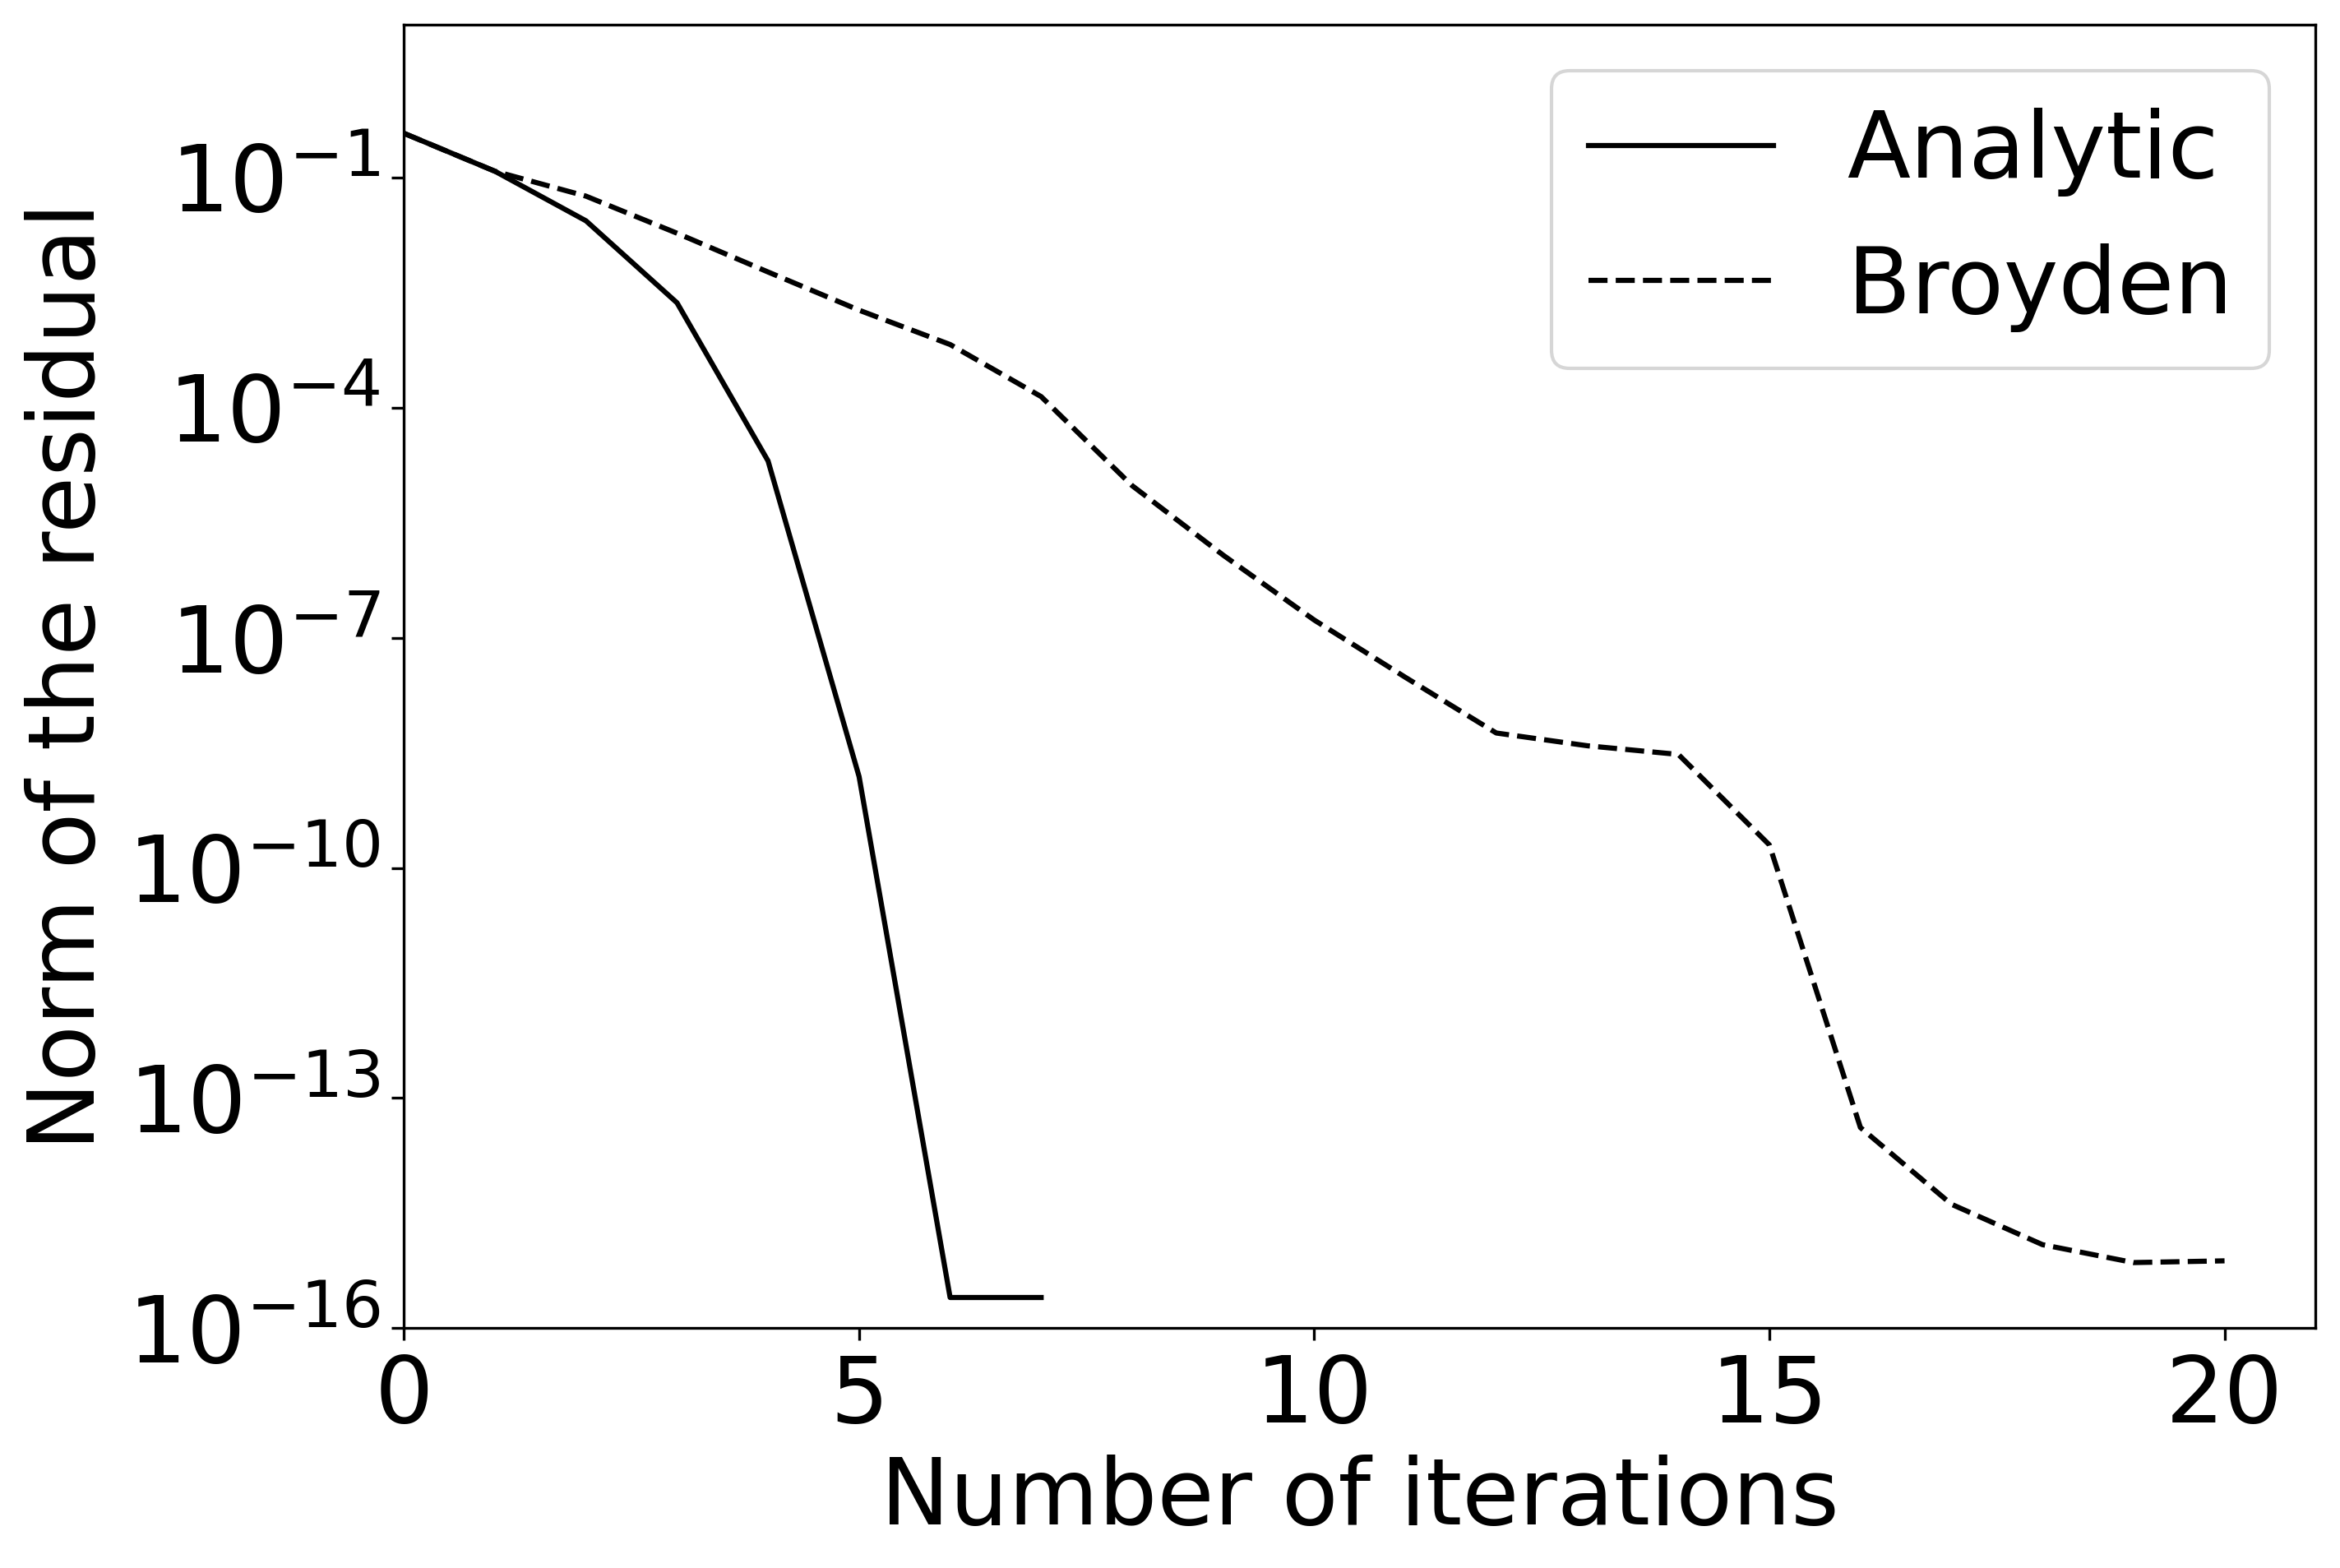
\includegraphics[width=0.9\textwidth]{images/NewtonIterationConvergence5Elements.png}
 		\subcaption{5 fault elements} 
 	\end{subfigure} 
 	\begin{subfigure}{0.32\textwidth}
 		\centering
 		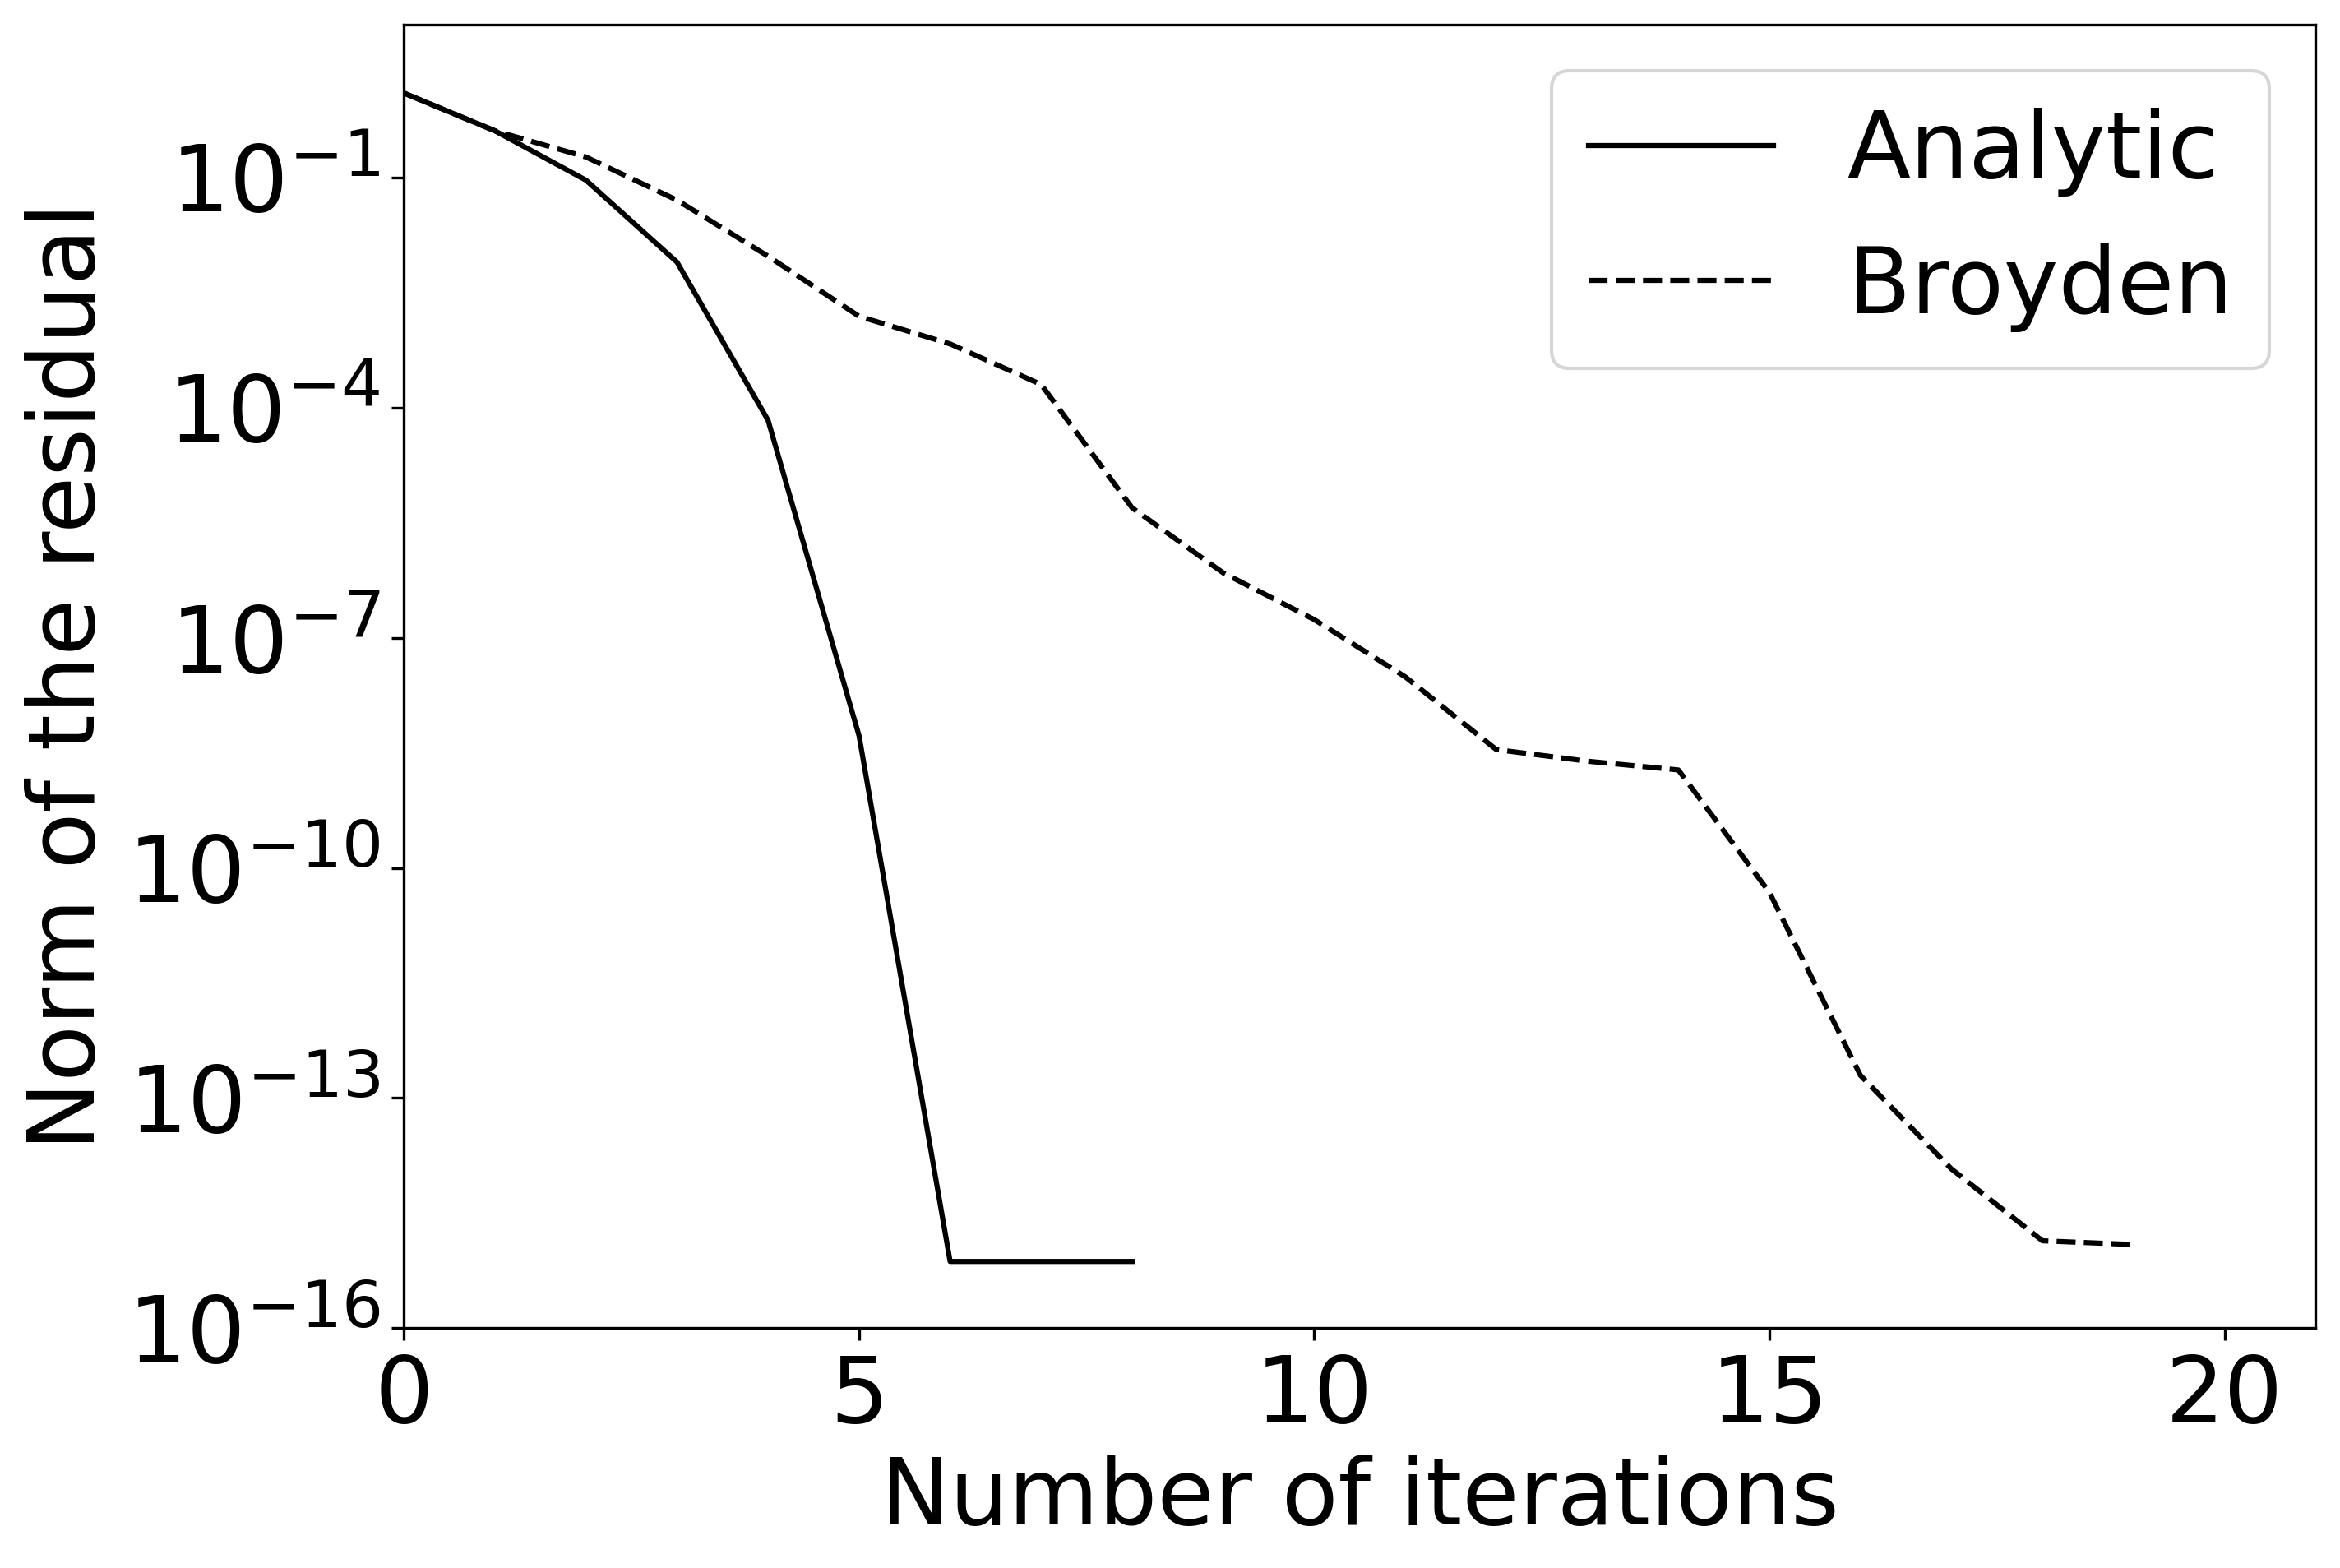
\includegraphics[width=1\textwidth]{images/NewtonIterationConvergence40Elements.png}
 		\subcaption{40 fault elements} 
 	\end{subfigure}
 	\begin{subfigure}{0.32\textwidth}
 		\centering
 		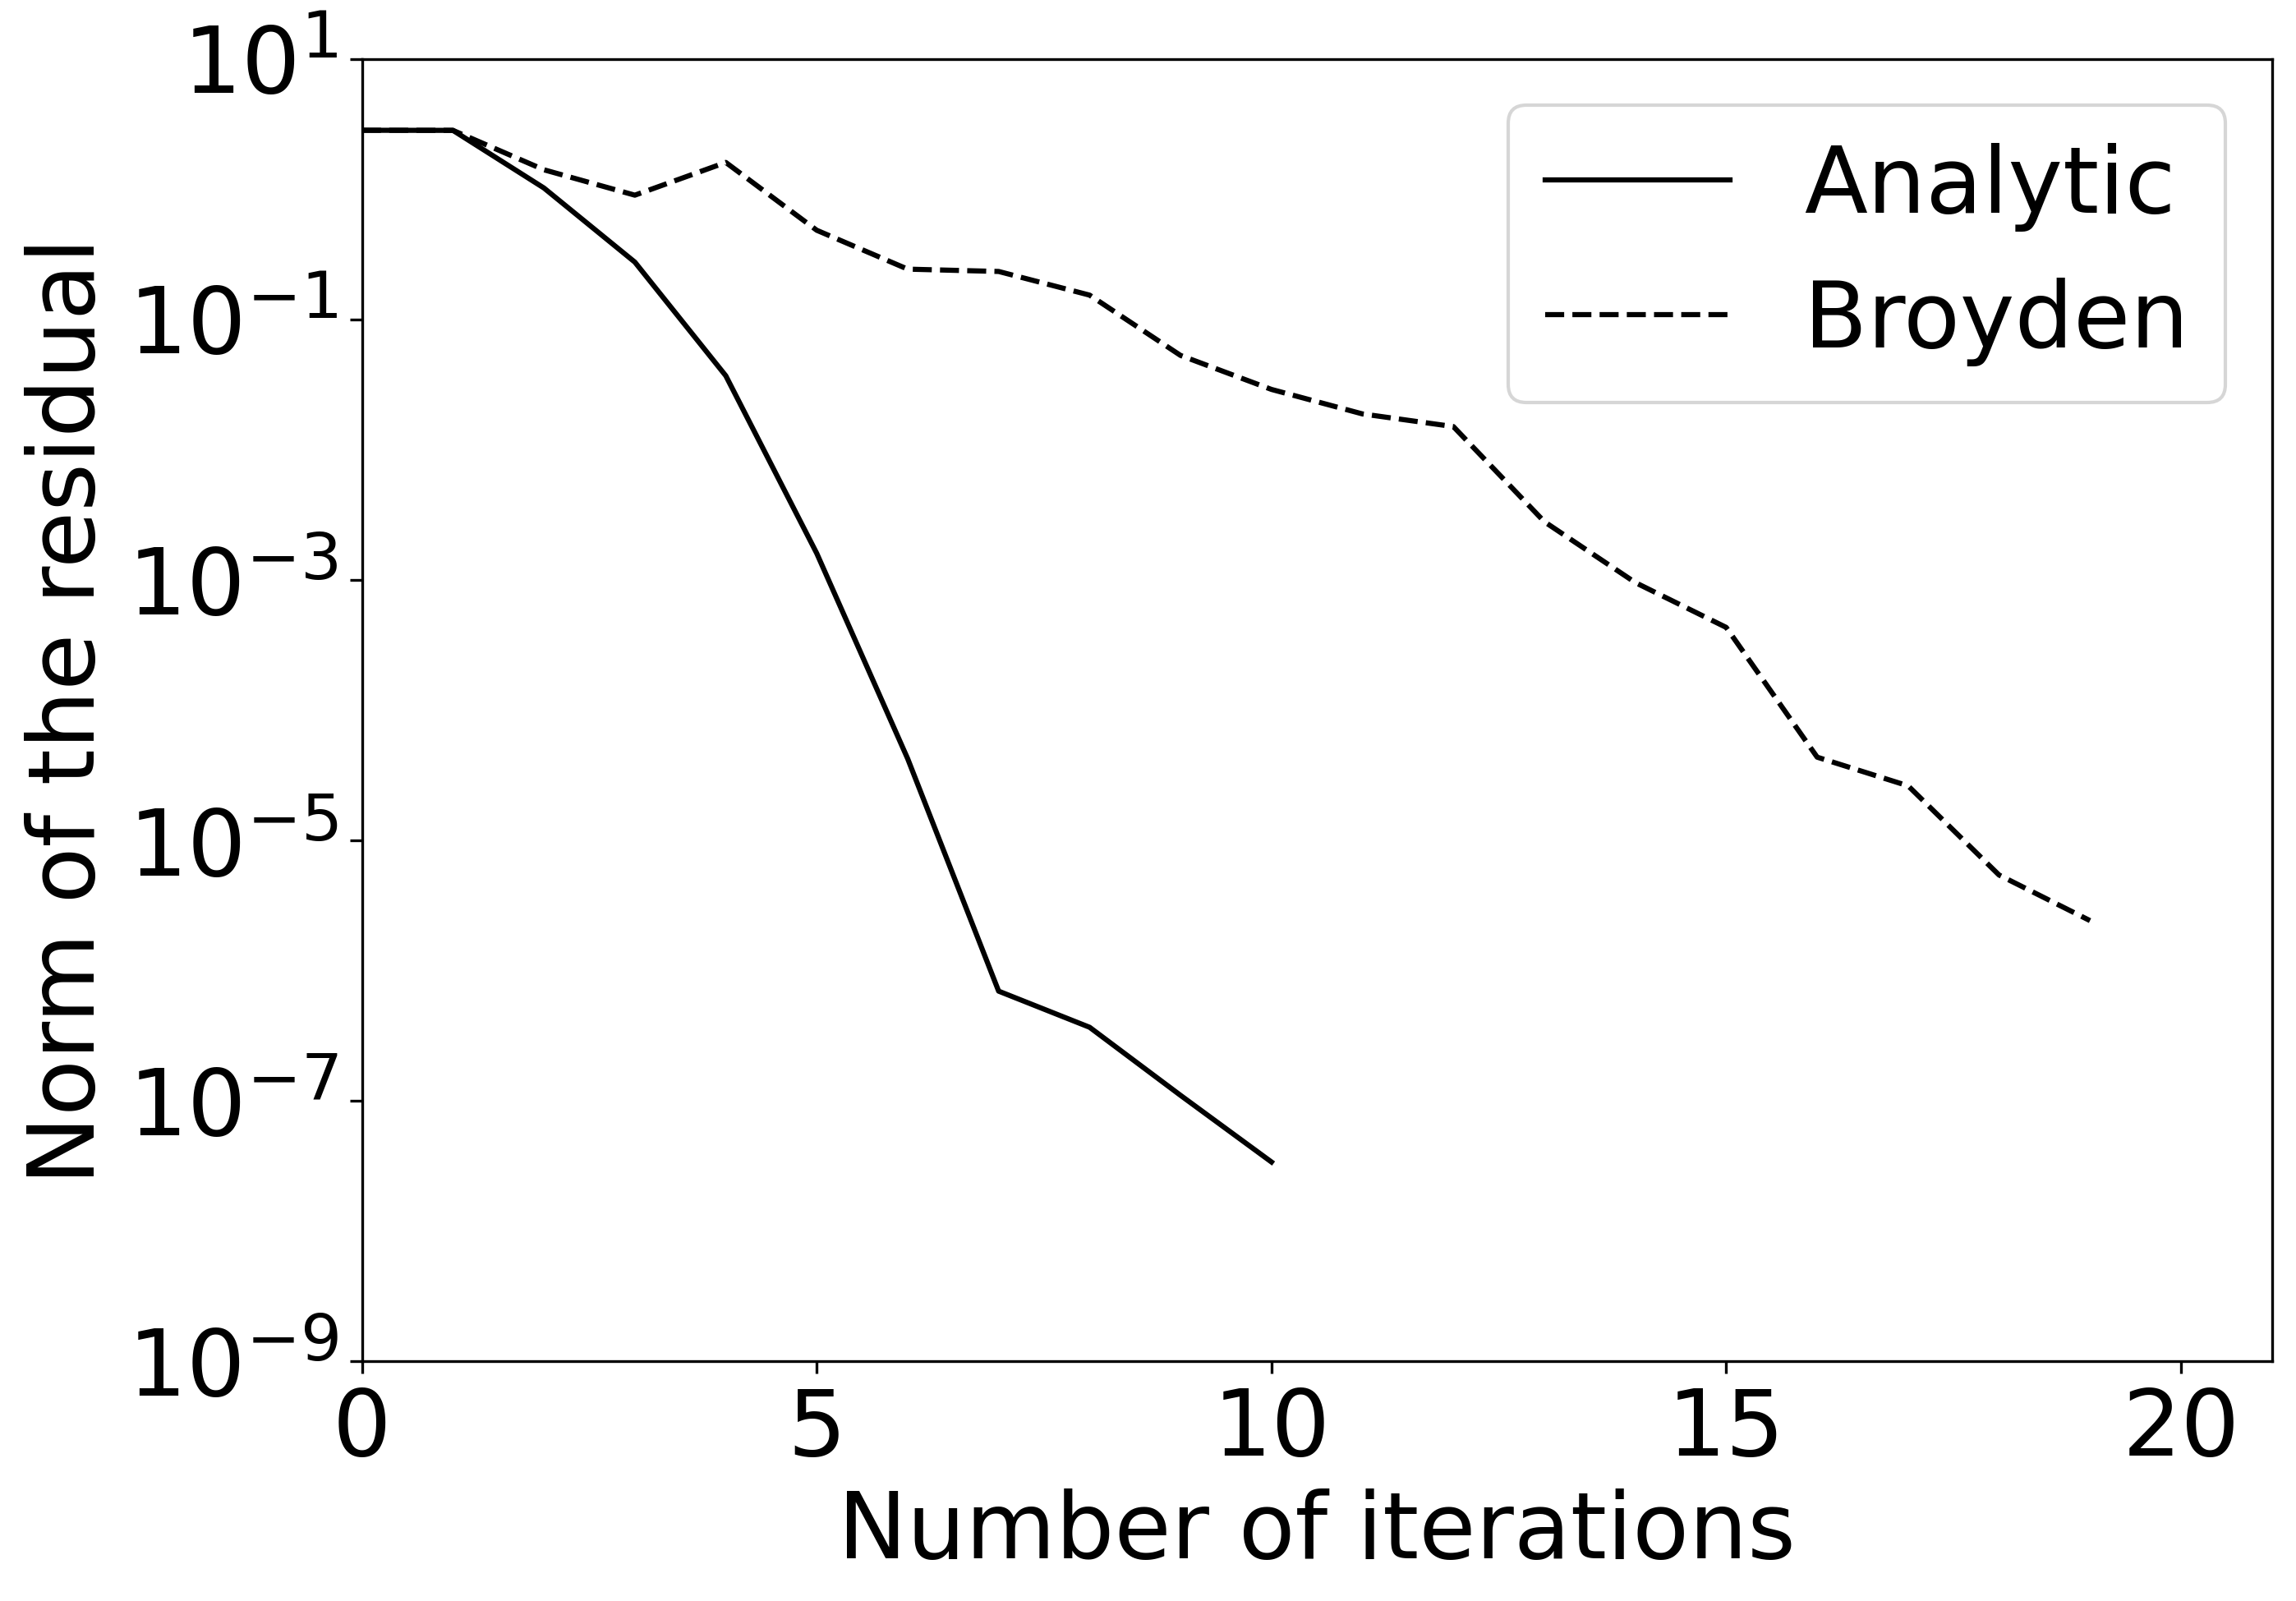
\includegraphics[width=1\textwidth]{images/NewtonIterationConvergence200Elements.png}
 		\subcaption{200 fault elements} 
 	\end{subfigure}
 	\caption{Evaluation of the L2 norm of the residual $\phi(x_n)$ at each iteration of the Newton and Broyden methods}
 	\label{fig:convergenceNewtonAndBroyden}
 \end{figure}
 It can be immediately seen that the Newton method with an analytical expression of the Jacobian reaches much faster the required tolerance of $10^{-8}$ as if it was approximated with the Broyden method. The convergence rate even seems to be quadratic, as one would expect for the Newton iteration. ???? Add some convergence test ????


\subsection{Limitations of the use of the Jacobian}
The main advantage of implicit methods over explicit methods is to allow larger time steps without loss in accuracy. The program execution is therewith expected to be accelerated. The proposed calculation of the Jacobian matrix and its application in Newton iterations comes along with some drawbacks with respect to the required calculation effort. \\
As described in \autoref{ssec:AnalyticalDerivationOfTheJacobianMatrix}, the computation of the Jacobian matrix can be split up in one constant part $\frac{\partial \tau_p}{\partial S_l}$ that has to be evaluated once at the beginning of the simulation and only depends on the domain geometry and in one variable part, that needs to be updated after each evaluation of the solution vector $x_n$. The initialization can be quite computationally expensive, at it requires, for each column of $\frac{\partial \tau_p}{\partial S_l}$, to solve the Discontinuous Galerkin system for the entire domain with the corresponding unit vector as right-hand side vector. Each calculation of this linear system is approximately as expensive as performing one time iteration with an explicit solver, since solving the same linear system is the most expensive operation of a time iteration. For large domains with several hundreds or thousands of fault elements, which each contains a couple of fault nodes, this initialization operation takes a considerable amount of time. In comparison with an explicit scheme, a potential implicit method starts the race for the fastest solver with a penalty of about $n$ explicit time iterations, where $n$ is the total number of nodes on the fault. The advantages of implicit methods will therefore only pay off after a high number of iterations and make such methods of interest only if the simulated time frame is very long. \\
Another potential drawback of the Newton method is that a linear system of size $n$ needs to be solved at each iteration step. This might still sound much less than solving for the displacement on the whole DG-domain of size $N$ as it is required to evaluate the right-hand side of the ODE at each iteration too. However, the DG system has a constant matrix $A$ whose LU-decomposition can be calculated once at the beginning of the simulation and each evaluation of the right-hand side only requires a backward substitution of complexity $\mathcal{O}\left(N^2\right)$. For the Jacobi matrix, such a pre.processing is not available since it changes along with the solution vector. Every calculation to solve the linear system in the Newton iteration is achieved with a complexity of the order $\mathcal{O}\left(n^3\right)$. In particular in large domains with many fault nodes the solver with cubic complexity may involve a substantially higher execution time than the one with quadratic complexity. Notwithstanding, for such large domains, the question has to be asked whether a direct solver is still appropriate or whether iterative solvers yield acceptable results. Such considerations are however beyond the scope of this thesis (so far ???).

\section{Numerical treatment in SEAS}
To solve this problem, the time solvers of the PETSc library [cite PETSc XXXX] are used. In general, they require a DAE of the form: 

\begin{equation}
    F(\dot{u}, u, t) = G(u, t)
\end{equation}

For SEAS, the solution vector $u$ combines the velocity $V$ and the state variable $\psi$ for all interpolation points at the edge of the fault elements. The functional $F$ is not used and takes as value only the time derivative of the solution vector $\dot{u}$. The call of the right-hand-side function $G(u,t)$ combines the solving of the algebraic and the differential equations. At each step, following steps are performed: 
\begin{enumerate}
    \item The current displacement in the whole system is calculated to fulfill the Poisson or elasticity equations by solving \autoref{eq:SEAS_DAE_AU=b} \\
    \item The values of $\tau(U)$ and $\sigma_n(U)$ are calculated on the fault according to the updated displacements \\
    \item The iteration over all interpolation points on the fault is performed. At each interpolation step: \begin{itemize}
        \item the velocity $V_i$ is obtained from the friction law in \autoref{eq:SEASDAE_frictionLaw} with the bisection method,
        \item and the actual right hand side $G(u,t)$ of the ODE is evaluated using equations \ref{eq:SEAS_DAE_ageing_law} and \ref{eq:SEASDAE_dV_dt}.
    \end{itemize}
\end{enumerate}


\subsection{Explicit methods to solve the DAE}
Runge-Kutta schemes with error correction term 
\begin{itemize}
    \item Bogacki-Shampine (RKBS3): 2nd order with 3rd order error correction \\
    \item Dormand-Prince (RKDP5): 4th order with 5th order error correction 
\end{itemize}

\subsection{Implicit methods to solve the DAE}


\section{Results}
The simulation is run over a period of 250 years, in which one earthquake occurs on June 13th of the 195th year. This event can be clearly observed in \autoref{fig:timeEvolutionTANDEM_V} which depicts the maximum slip rate over time, which reaches $4.6m\cdot s^{-1}$ as opposed to an average of $1.0 \cdot 10^{-9}m\cdot s^{-1}$ in calm times. 
\begin{figure}[H]
    \centering
    \begin{subfigure}{0.32\textwidth}
    	\centering
    	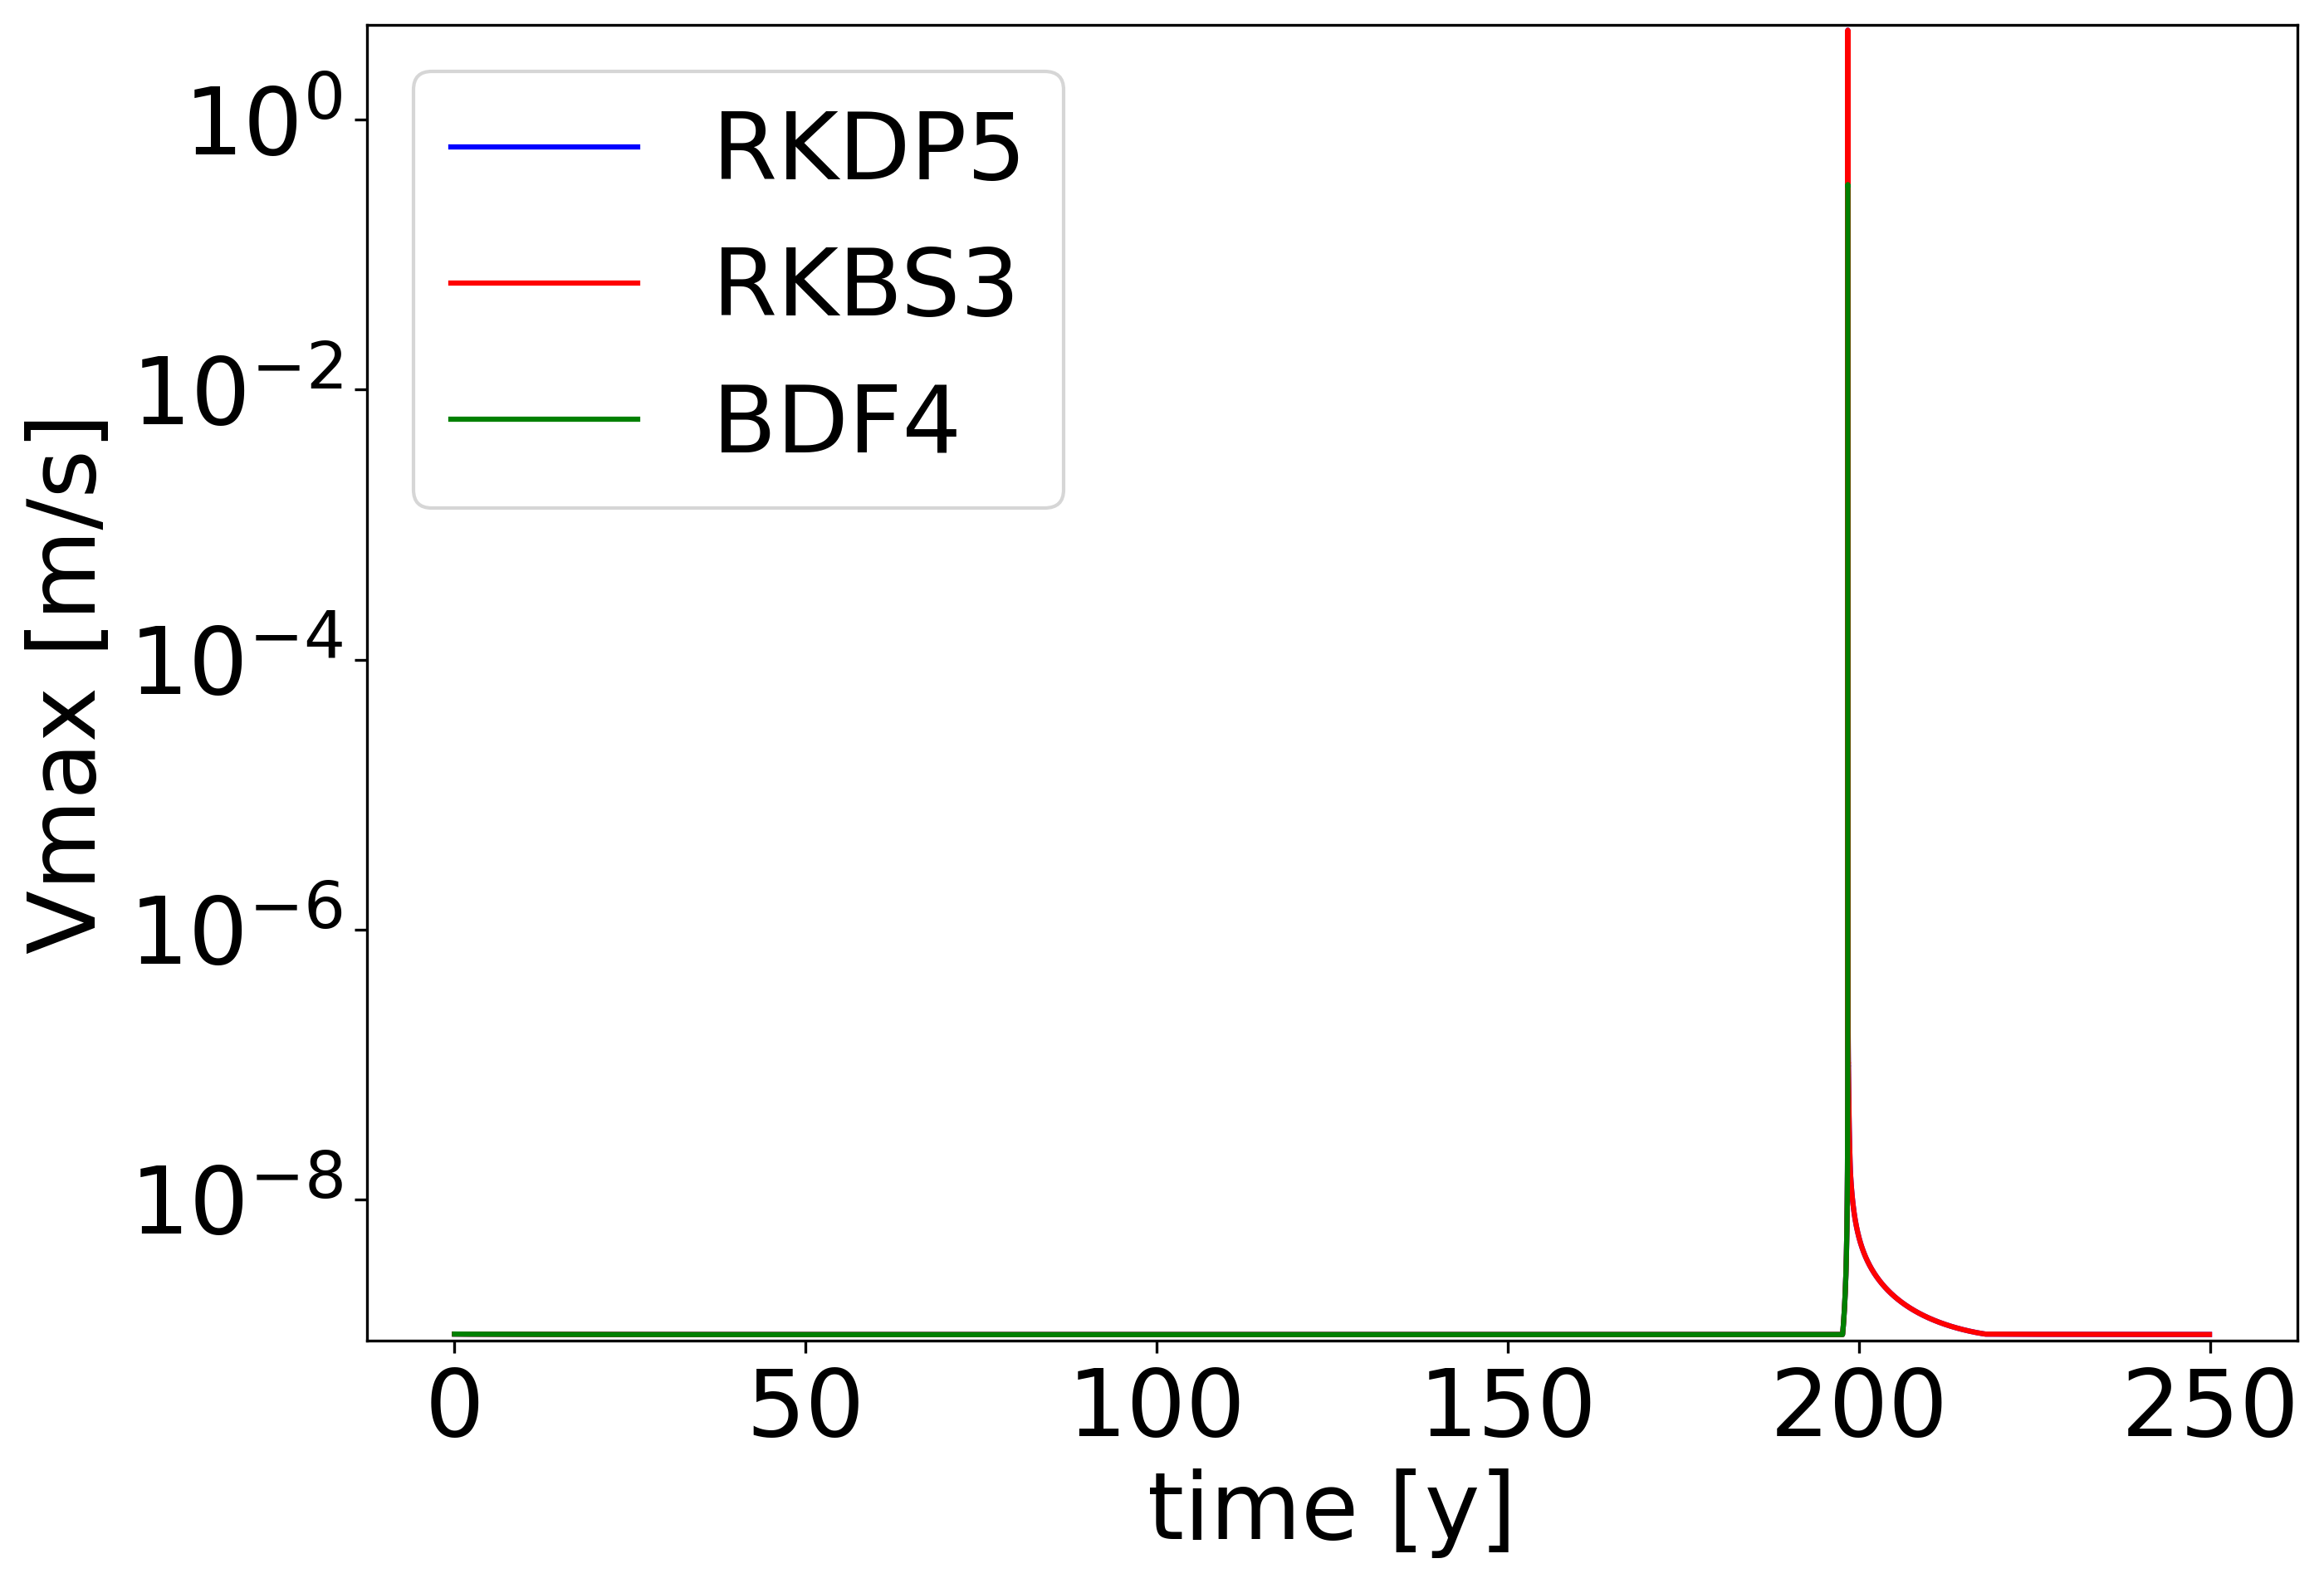
\includegraphics[width=1\textwidth]{images/TANDEMtimeEvolutionVall.png}
       	\subcaption{Full simulation time} 
    \end{subfigure} 
    \begin{subfigure}{0.32\textwidth}
    	\centering
    	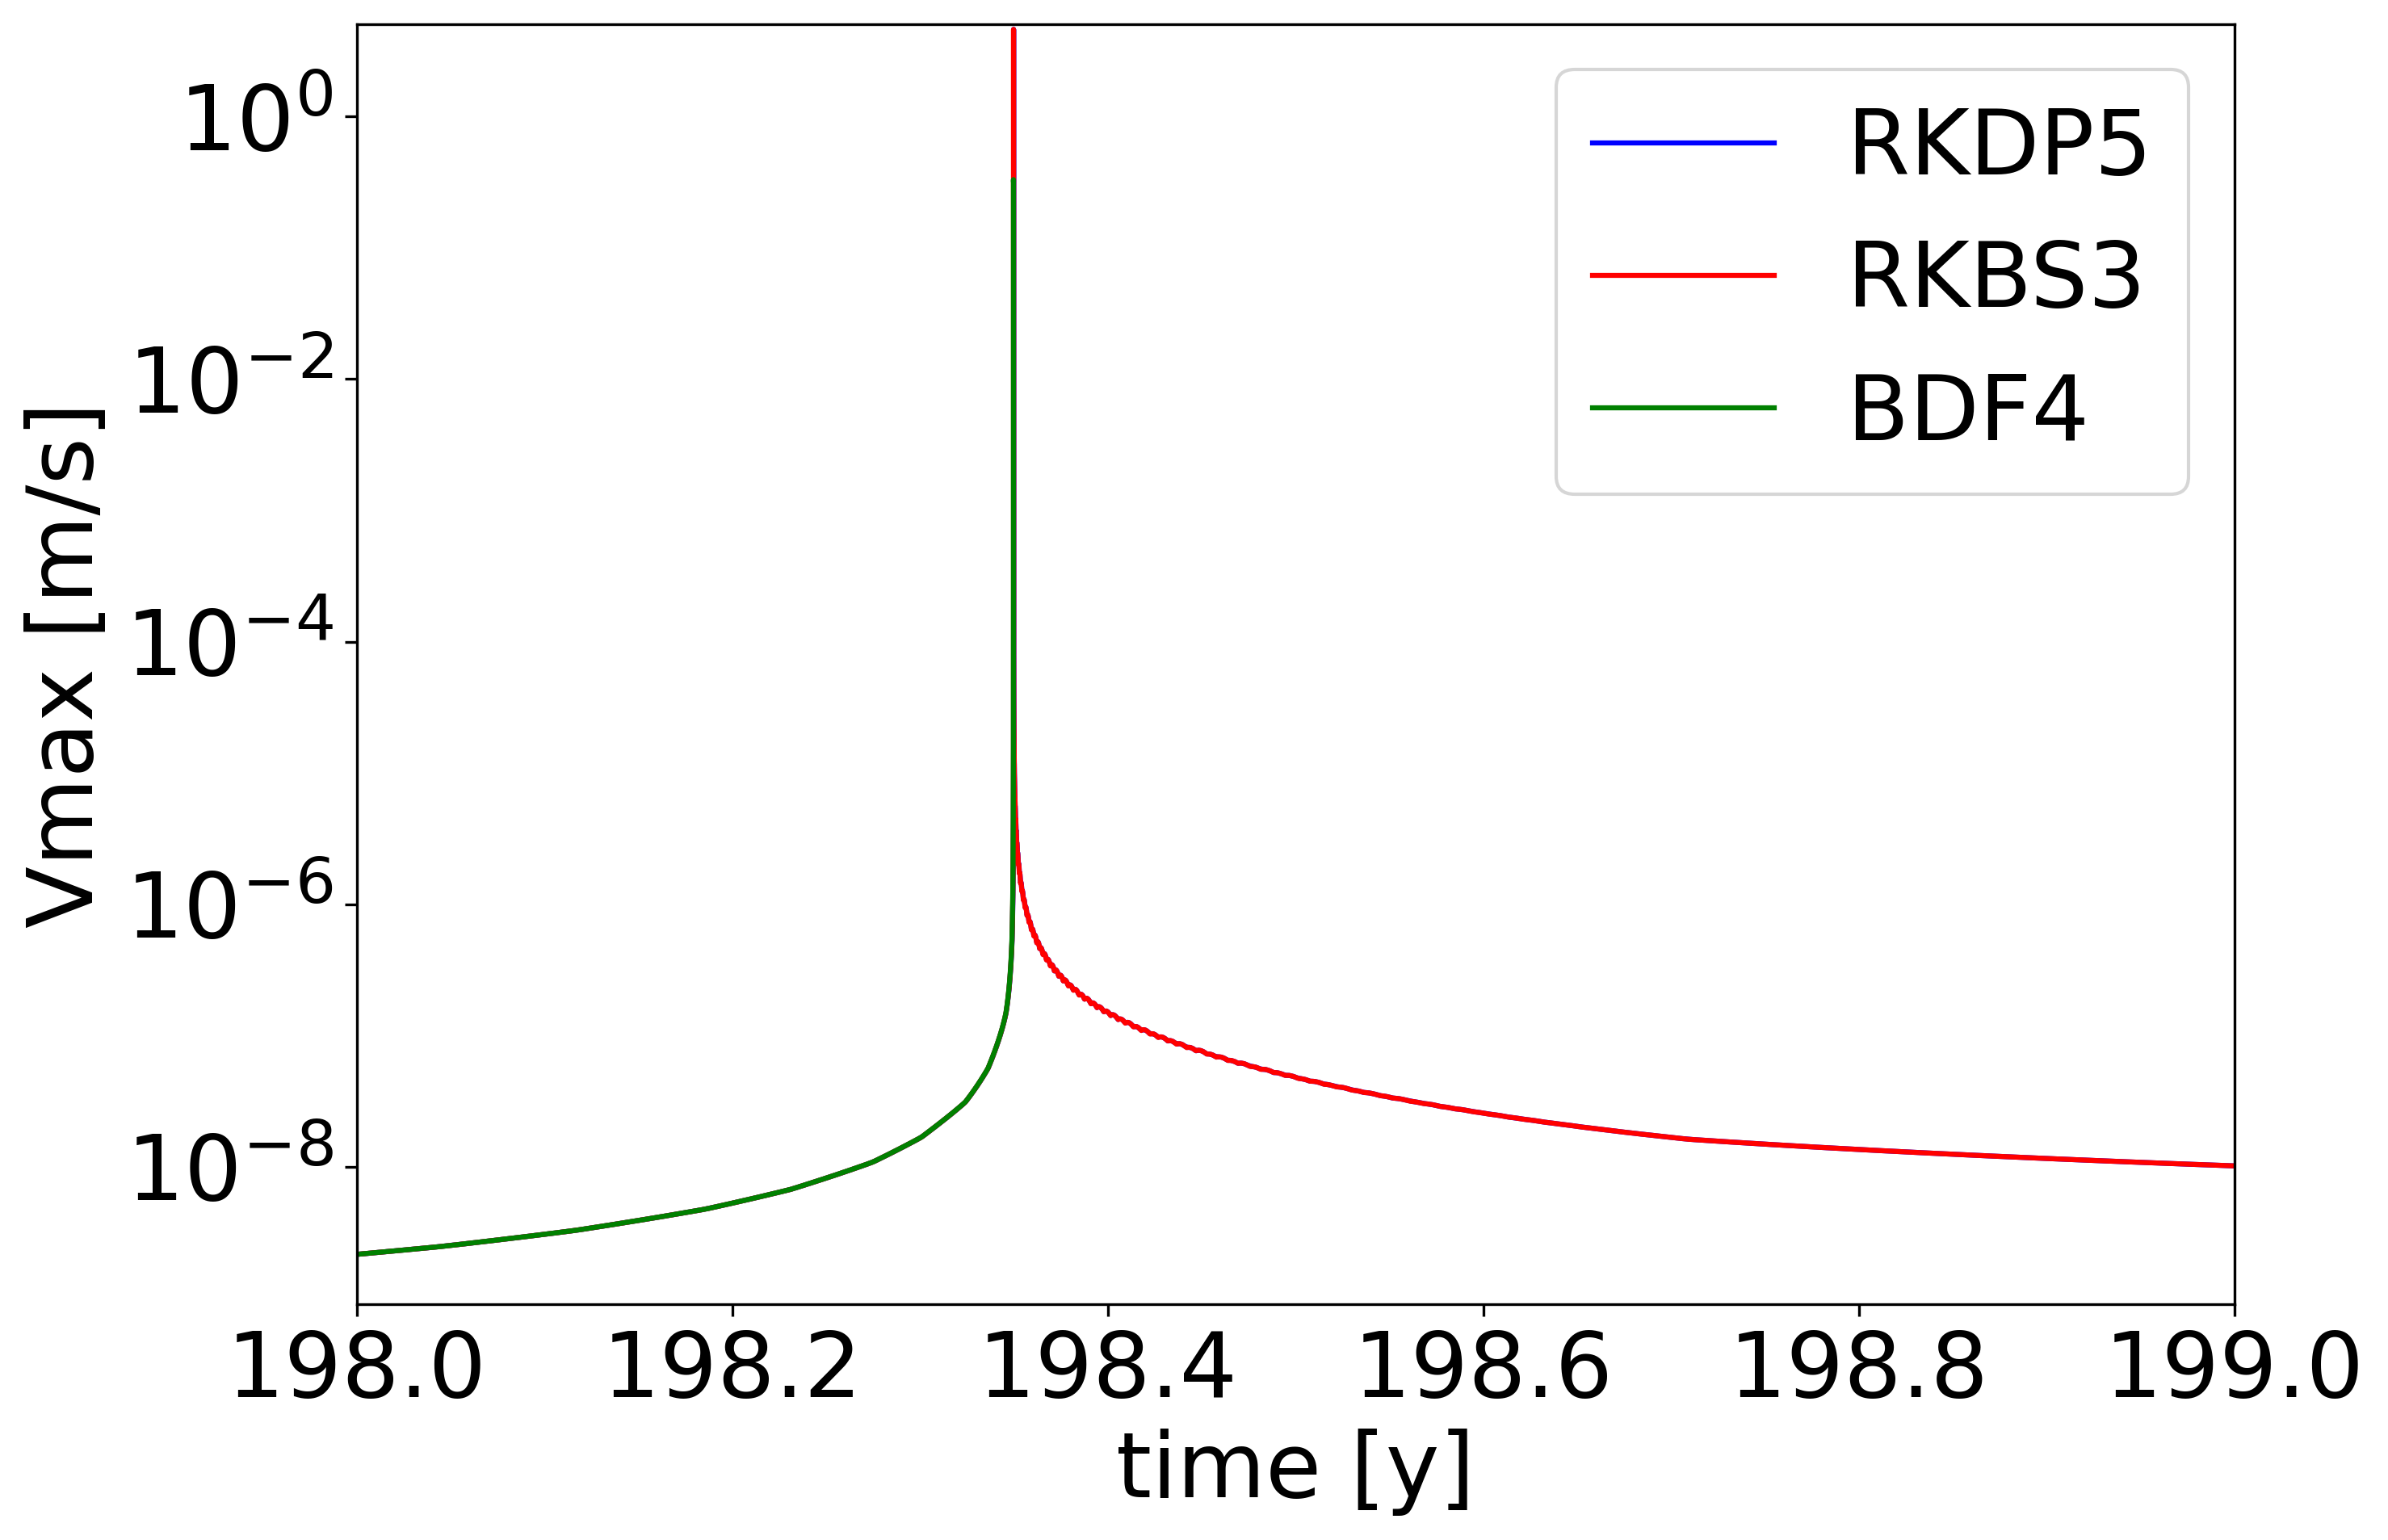
\includegraphics[width=1\textwidth]{images/TANDEMtimeEvolutionVsurroundings.png}
       	\subcaption{Year of the earthquake} 
    \end{subfigure}
    \begin{subfigure}{0.32\textwidth}
    	\centering
    	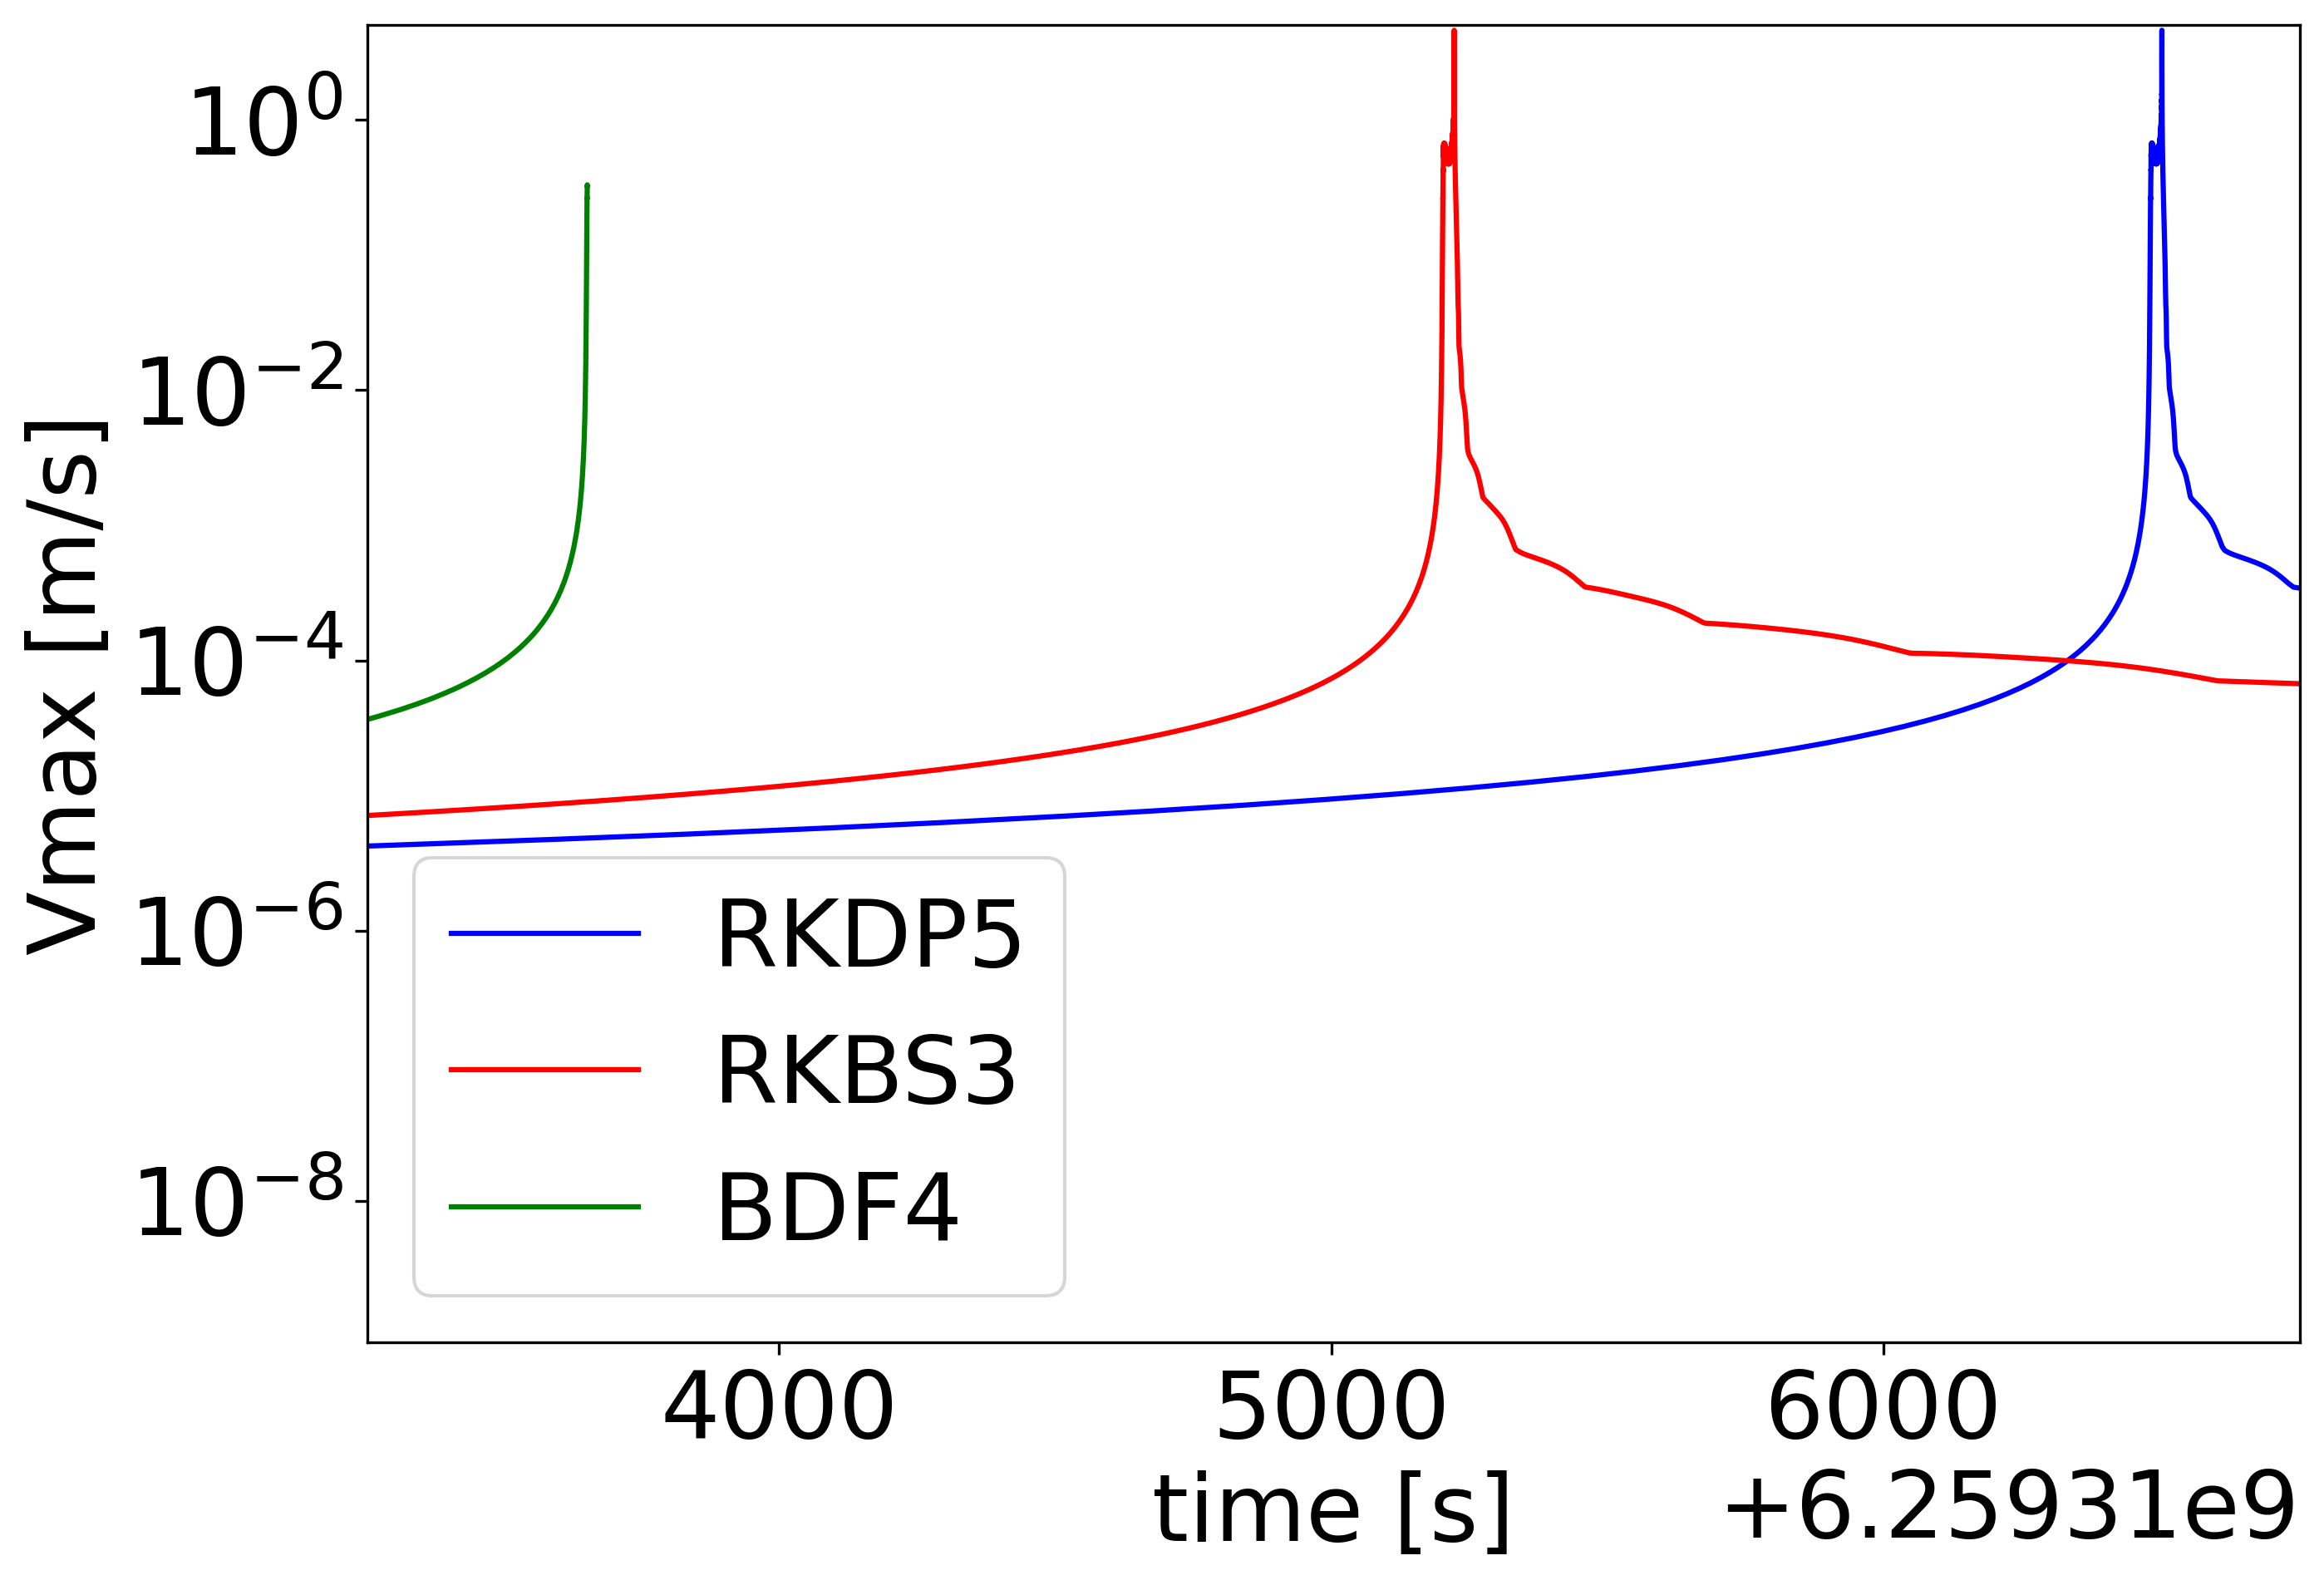
\includegraphics[width=1\textwidth]{images/TANDEMtimeEvolutionVearthquake.png}
       	\subcaption{Evolution of the earthquake event} 
    \end{subfigure}
    \caption{Evolution of the maximal slip rate $V$ on the fault for different solvers on the symmetric two-dimensional BP1 problem with 200 elements on the fault}
    \label{fig:timeEvolutionTANDEM_V}
\end{figure}


\begin{figure}[H]
    \centering
    \begin{subfigure}{0.32\textwidth}
    	\centering
    	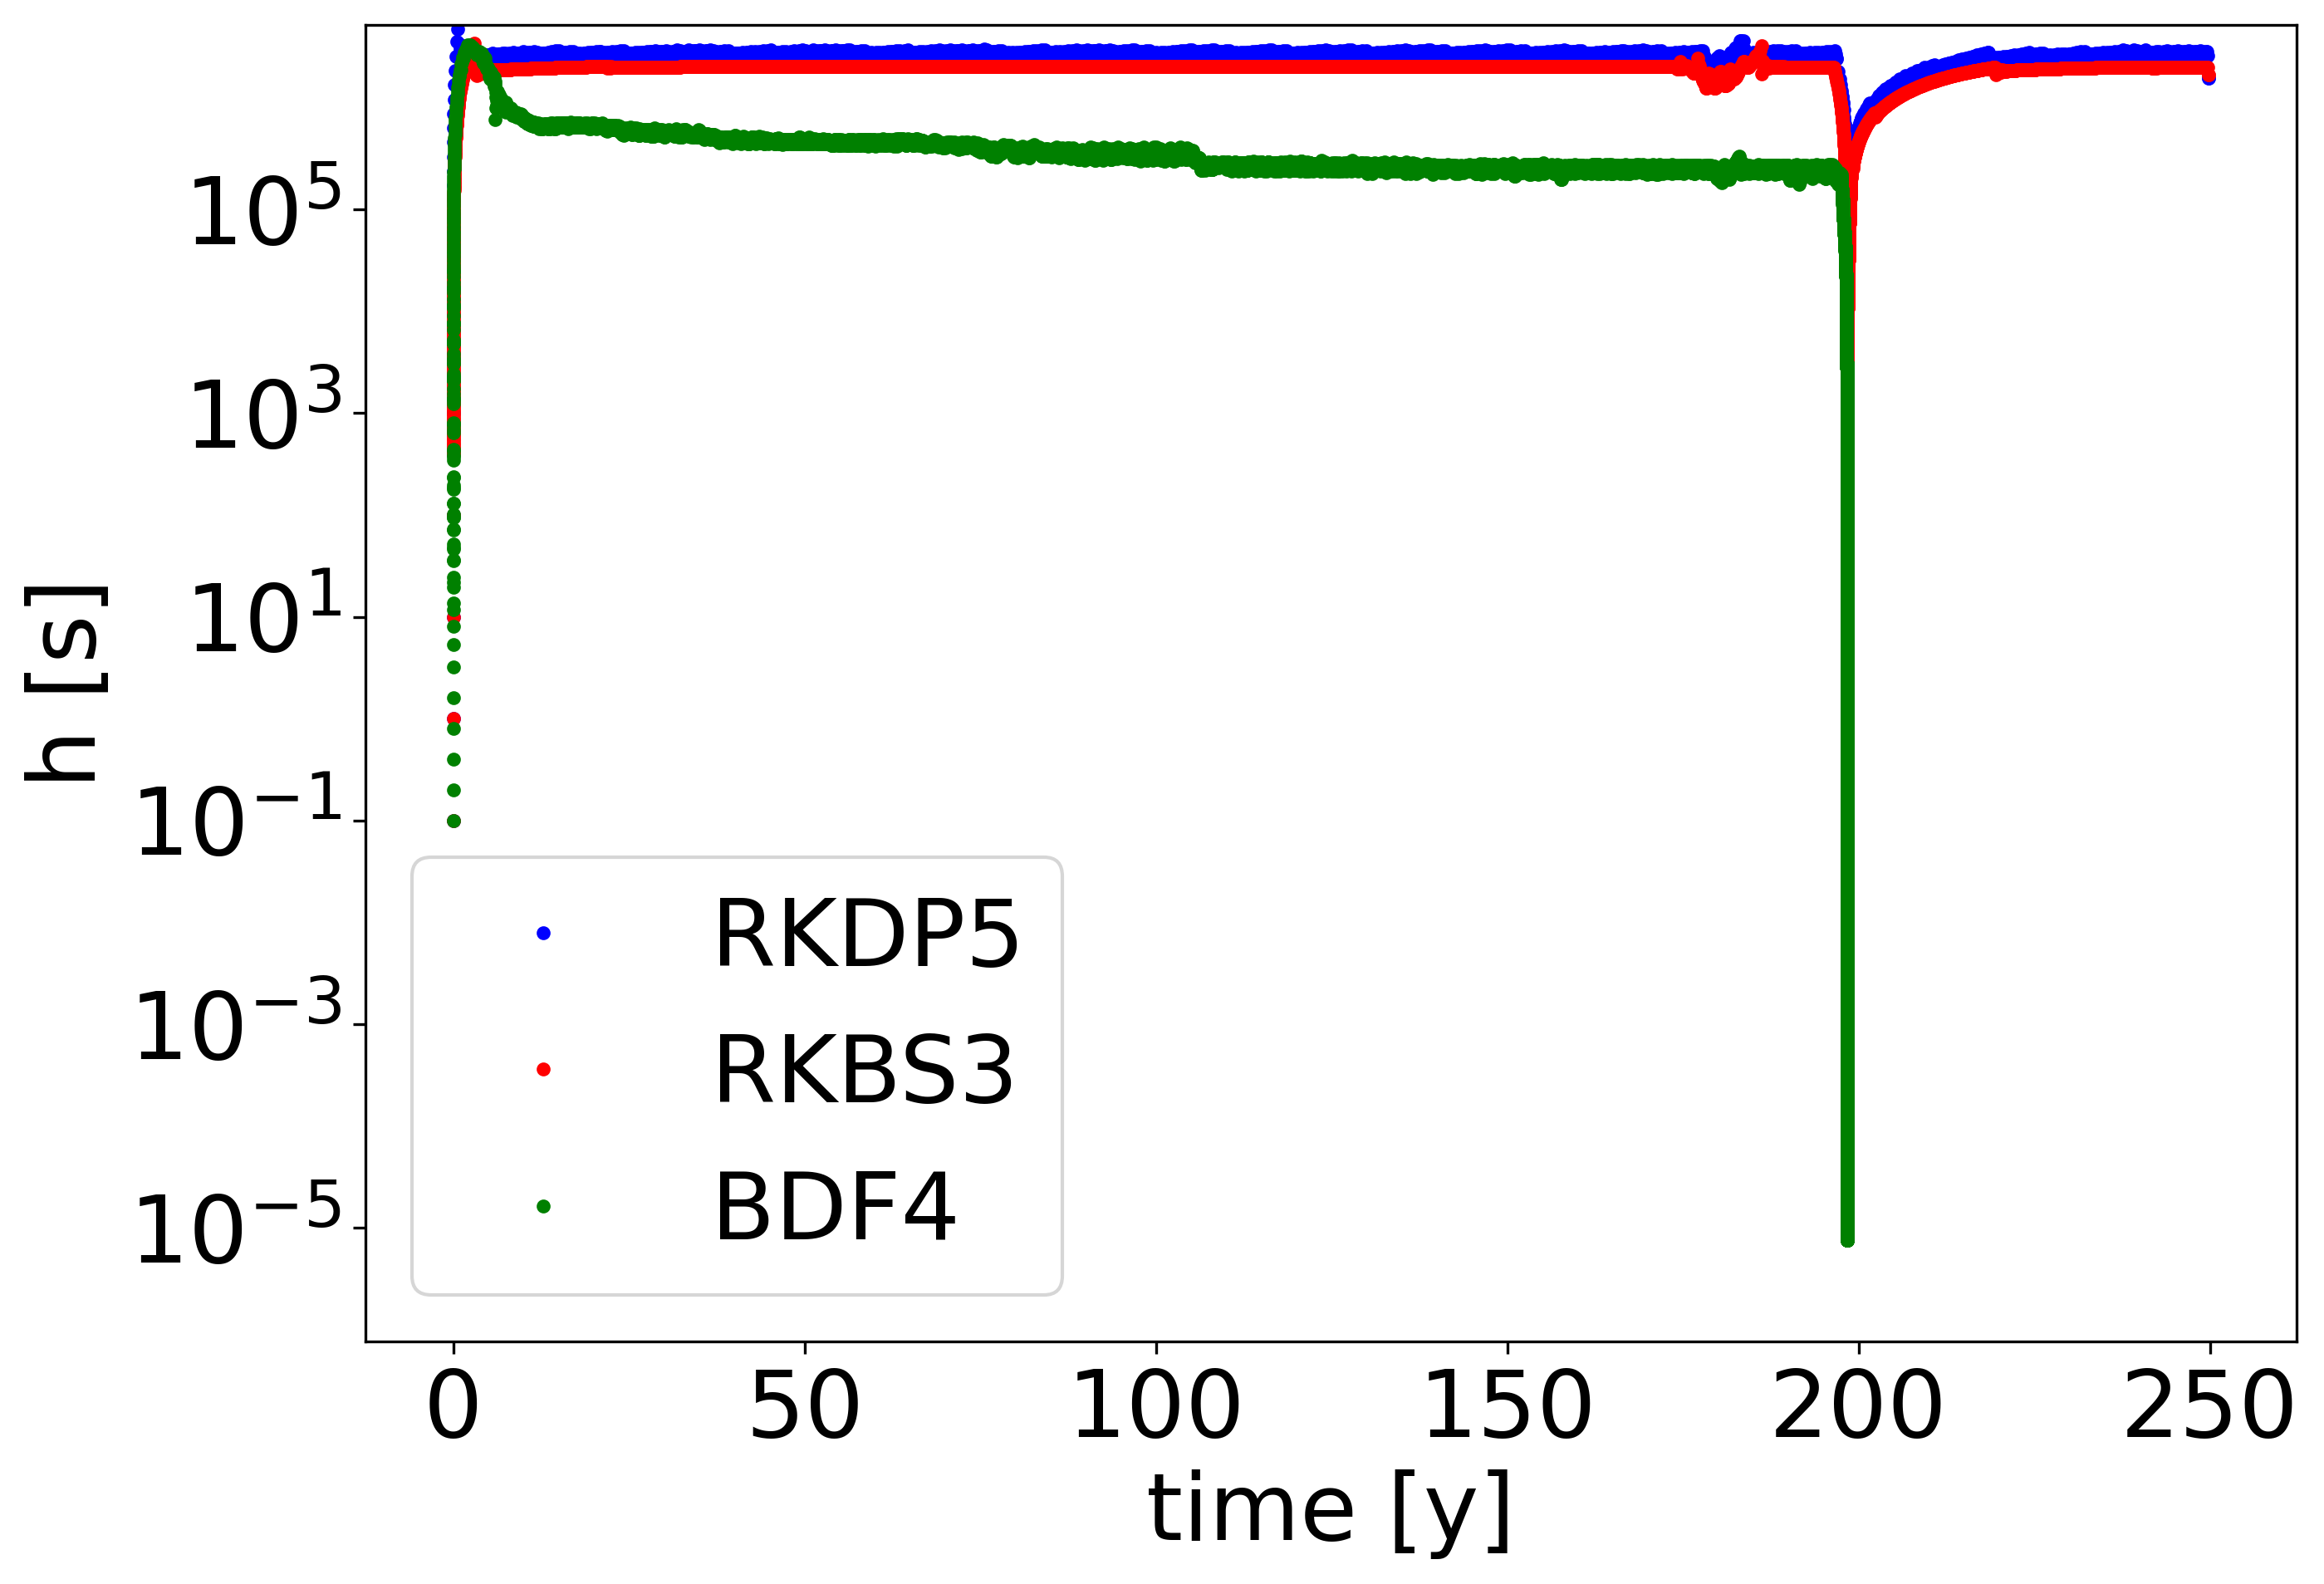
\includegraphics[width=1\textwidth]{images/TANDEMtimeEvolutionDTall.png}
       	\subcaption{Full simulation time} 
    \end{subfigure}
    \begin{subfigure}{0.32\textwidth}
    	\centering
    	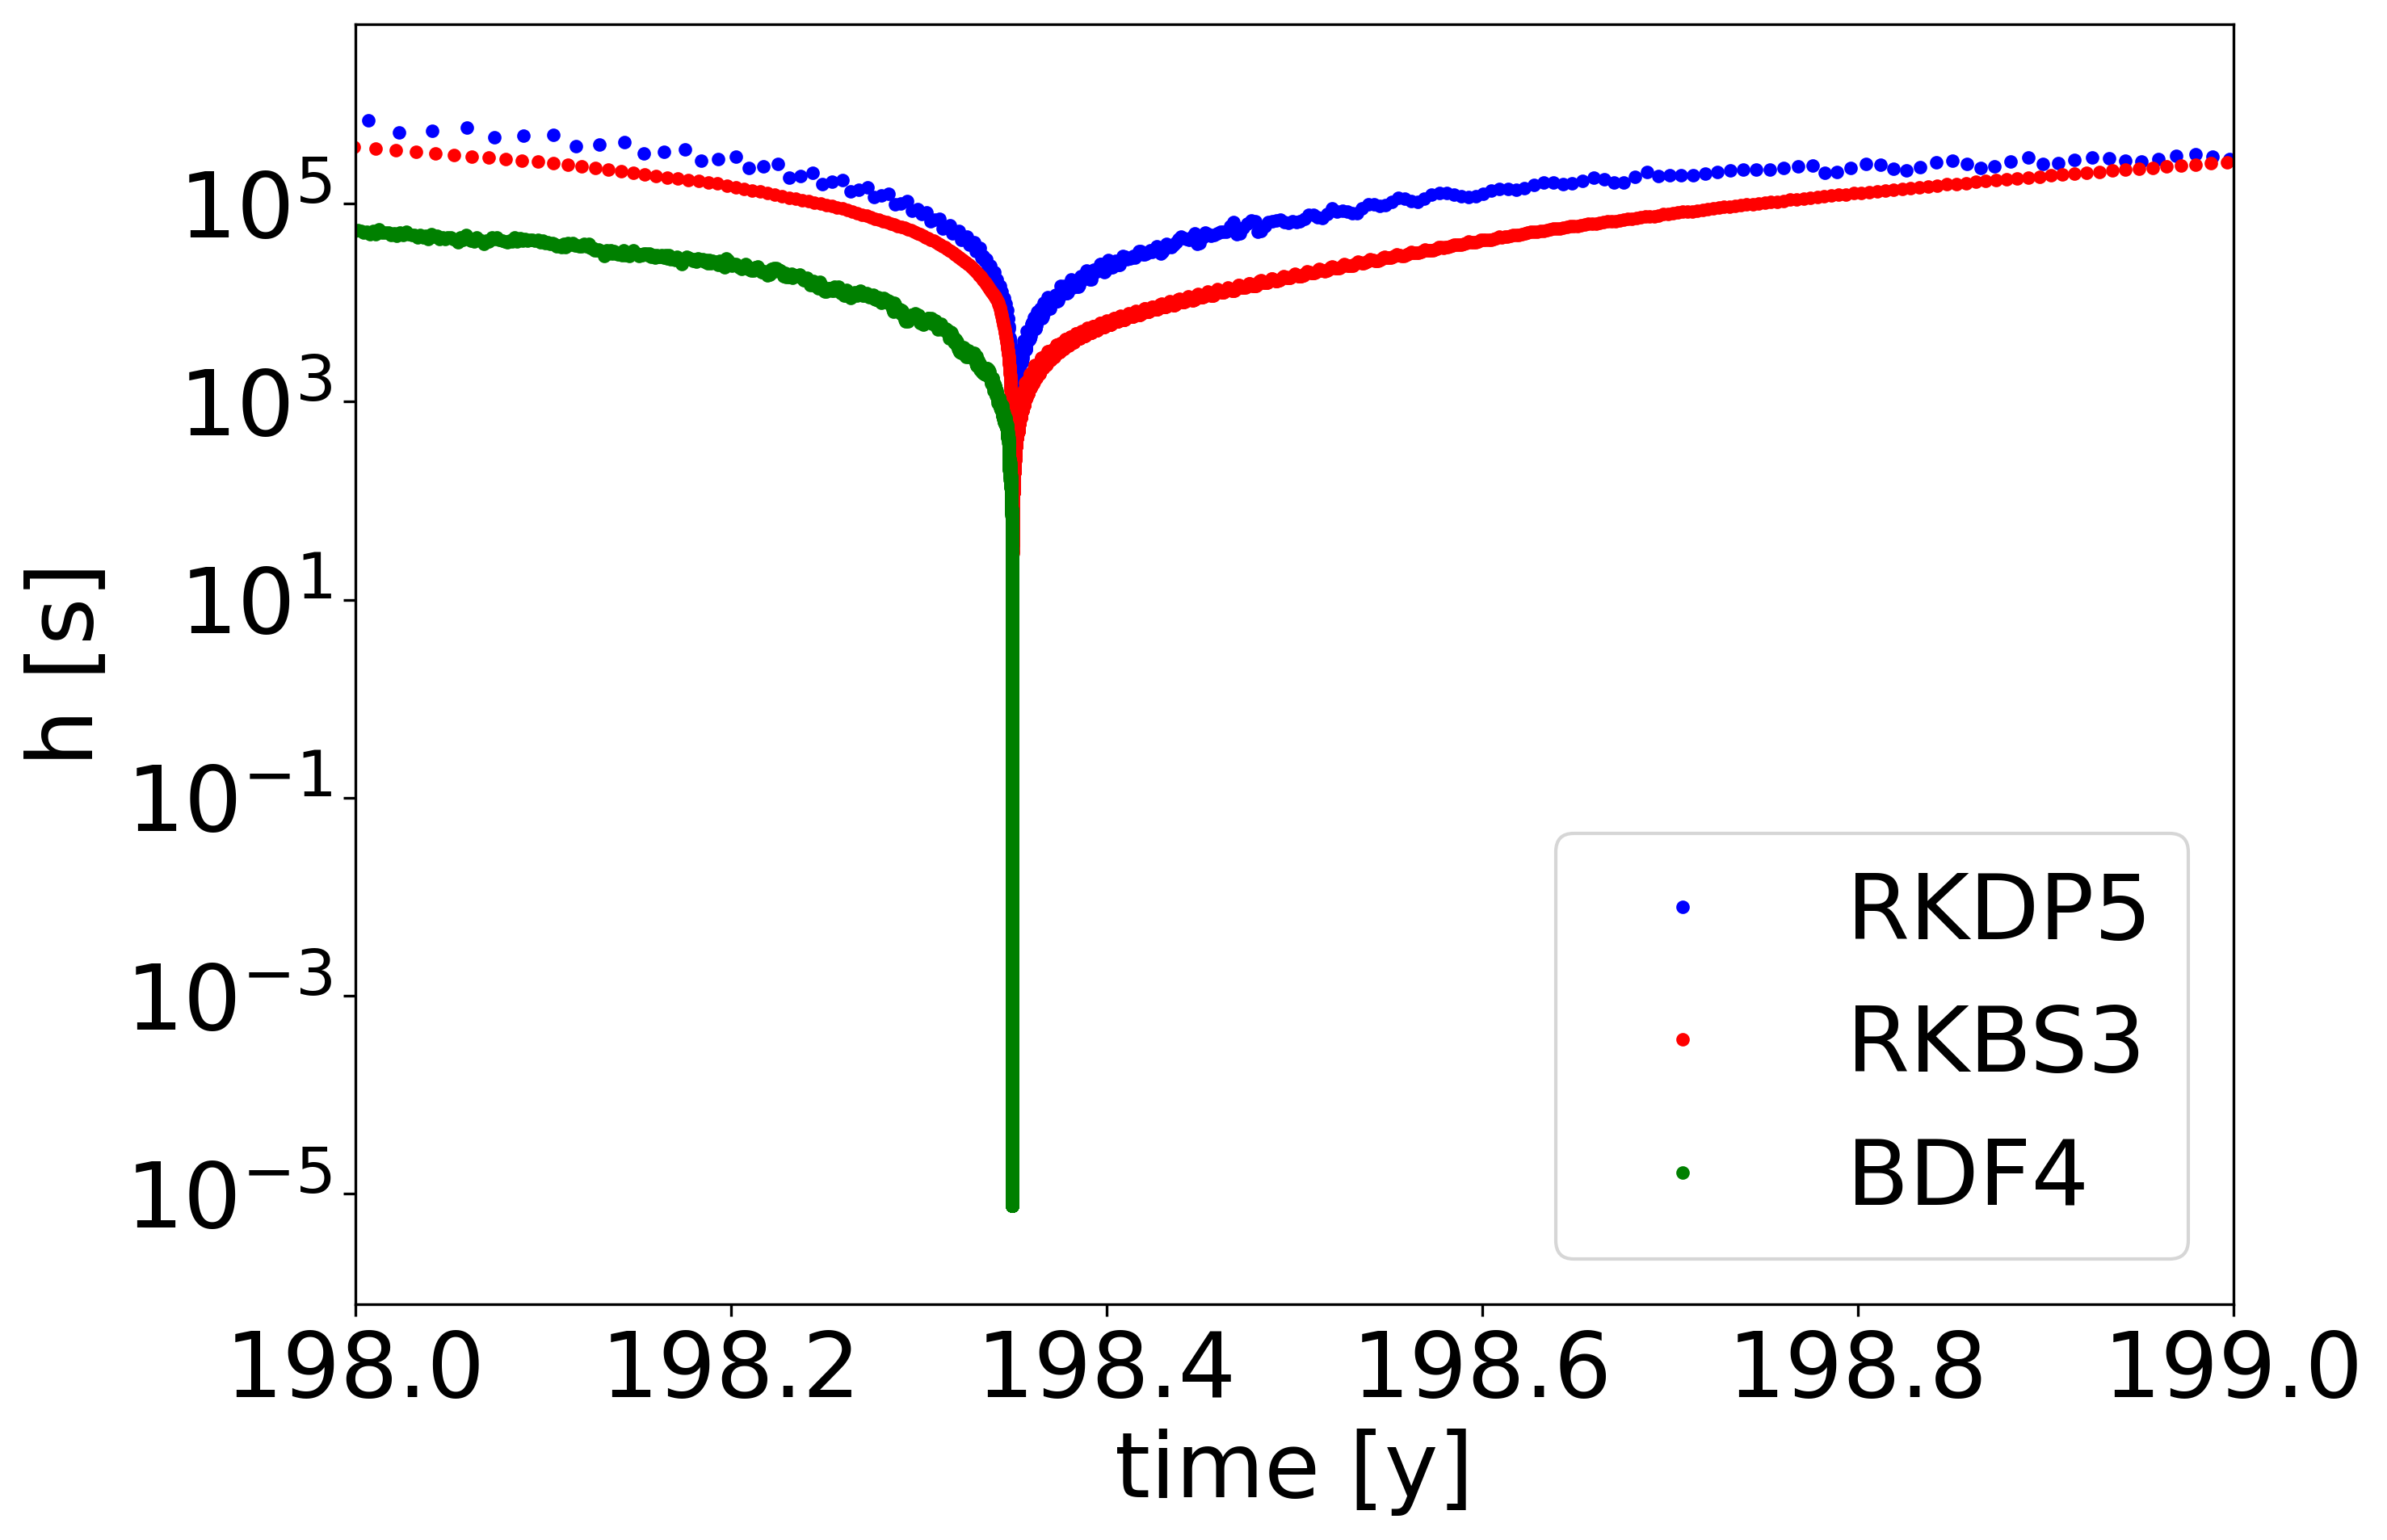
\includegraphics[width=1\textwidth]{images/TANDEMtimeEvolutionDTsurroundings.png}
       	\subcaption{Year of the earthquake} 
    \end{subfigure}
    \begin{subfigure}{0.32\textwidth}
    	\centering
    	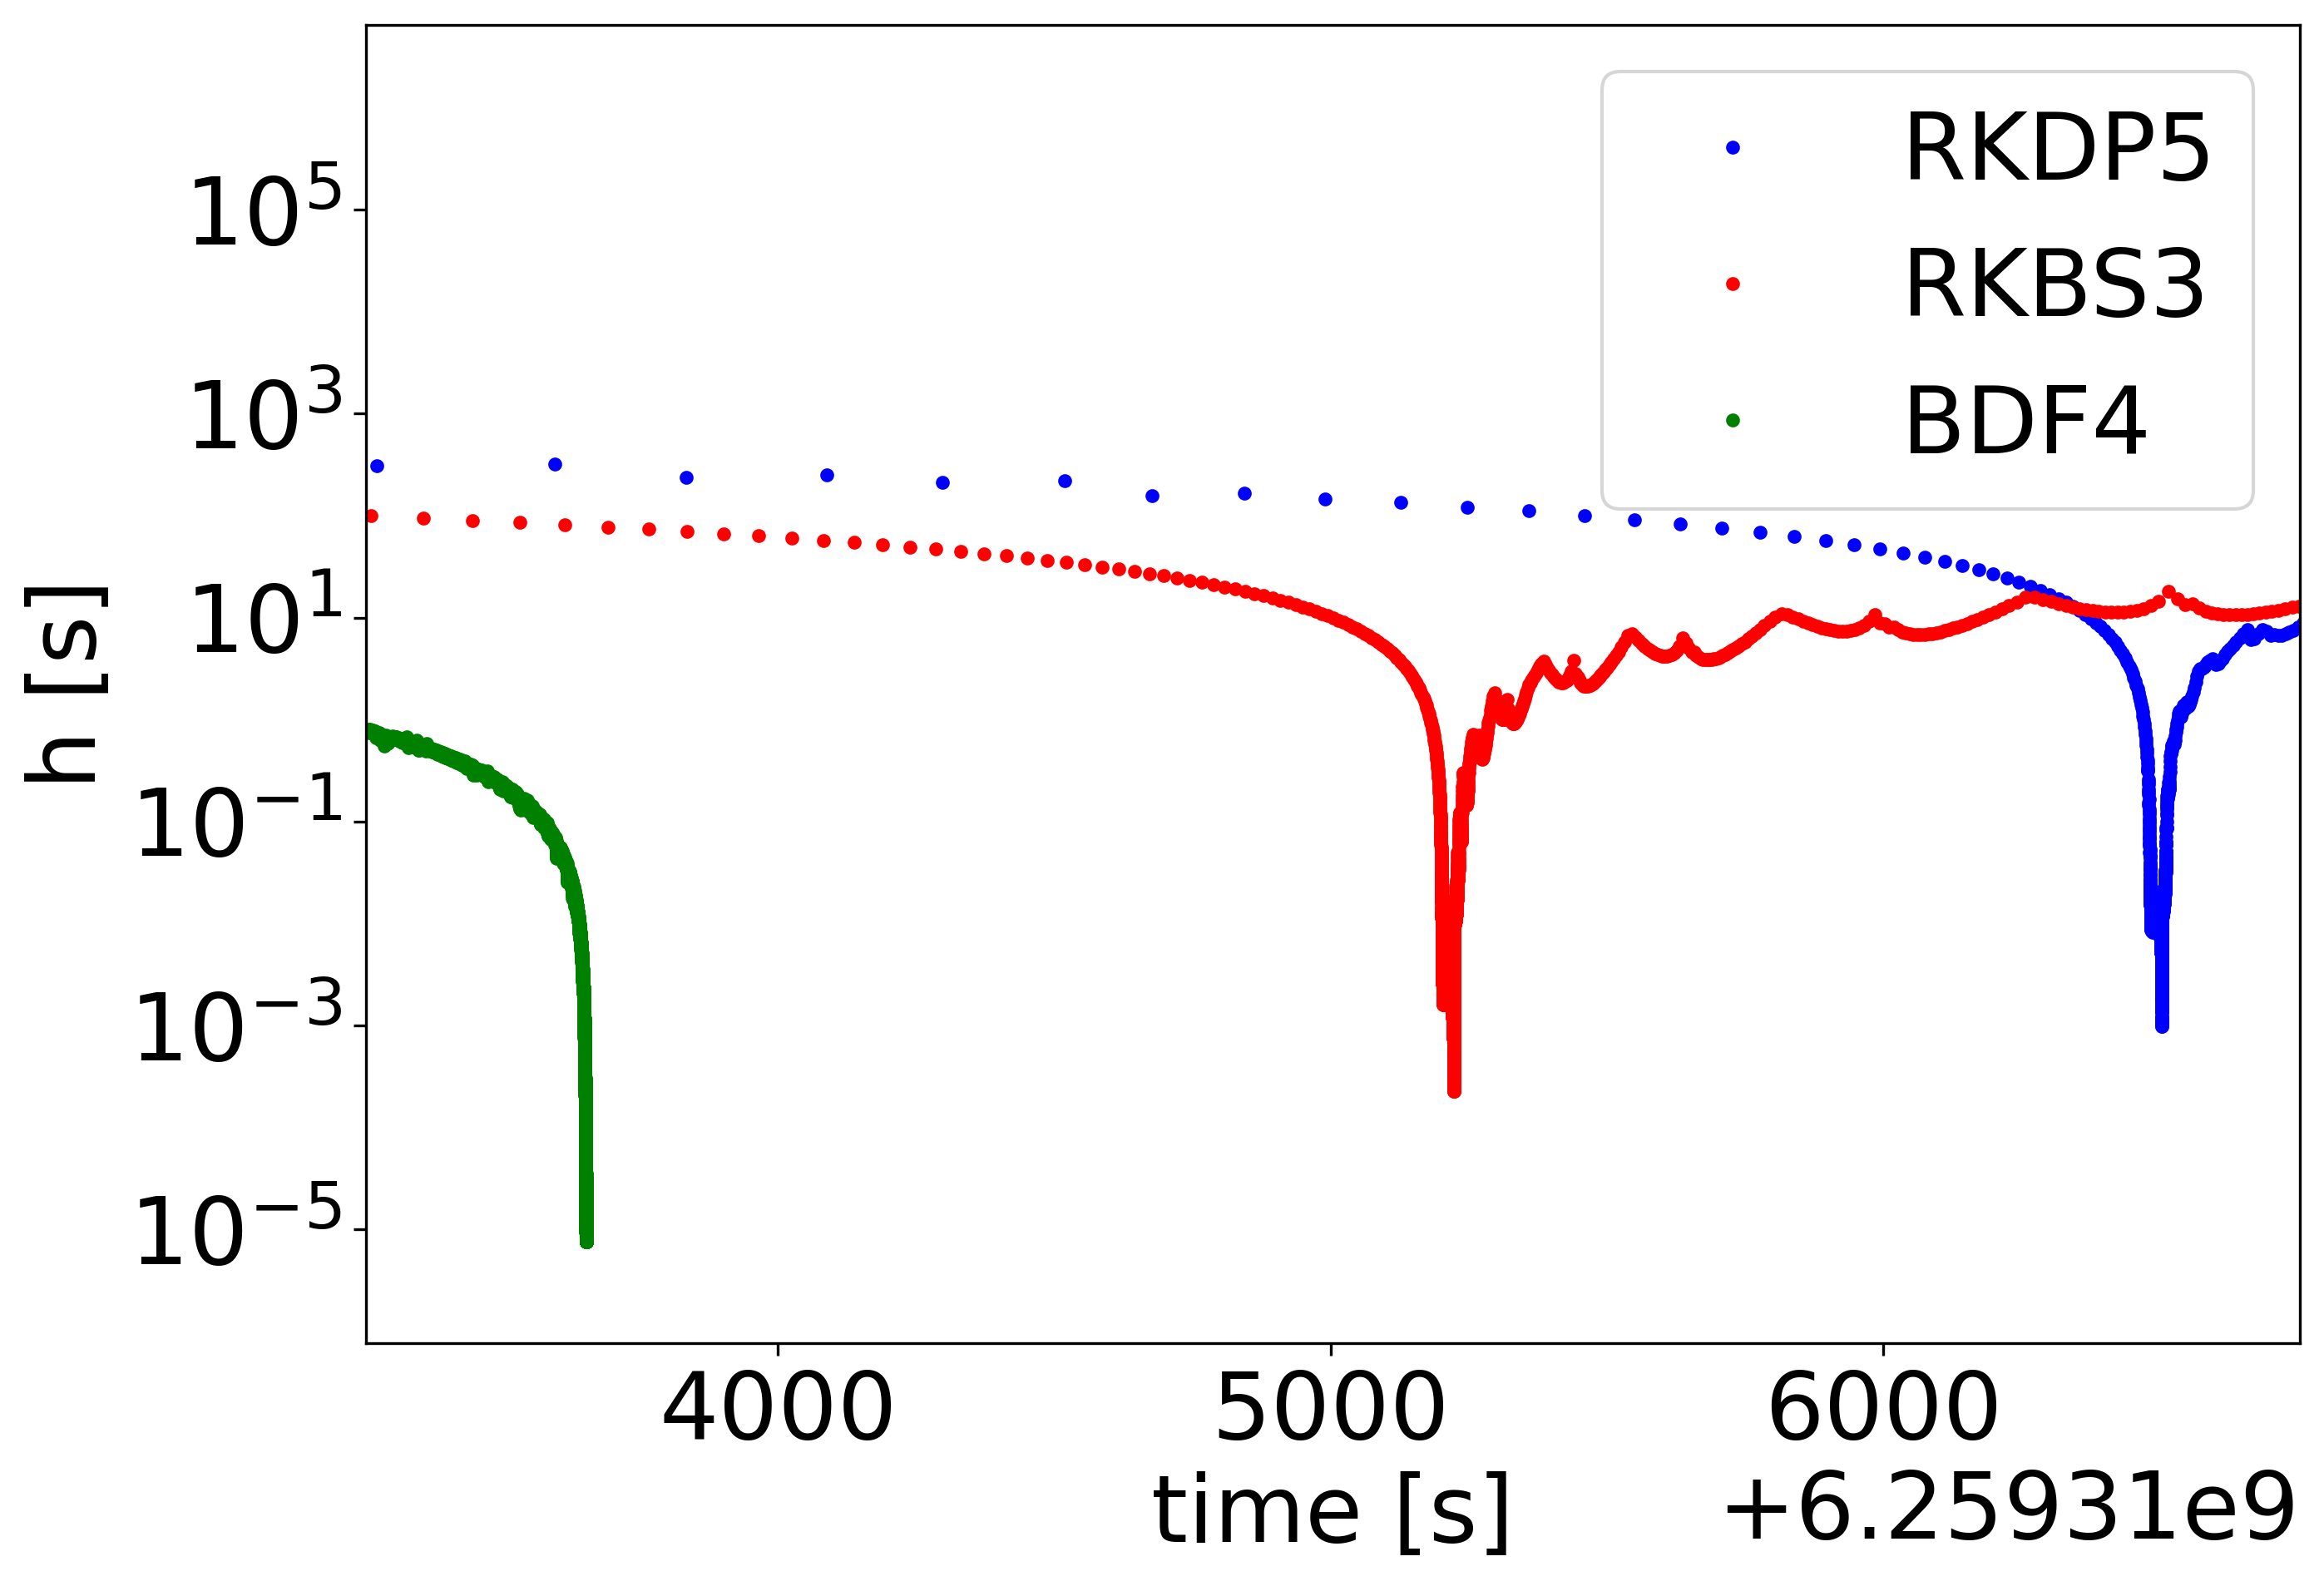
\includegraphics[width=1\textwidth]{images/TANDEMtimeEvolutionDTearthquake.png}
       	\subcaption{Evolution of the earthquake event} 
    \end{subfigure}
    \caption{Evolution of the time step size $h$ for different solvers on the symmetric two-dimensional BP1 problem with 200 elements on the fault}
    \label{fig:timeEvolutionTANDEM_DT}
\end{figure}


\begin{figure}[H]
    \centering
    \begin{subfigure}{0.32\textwidth}
    	\centering
    	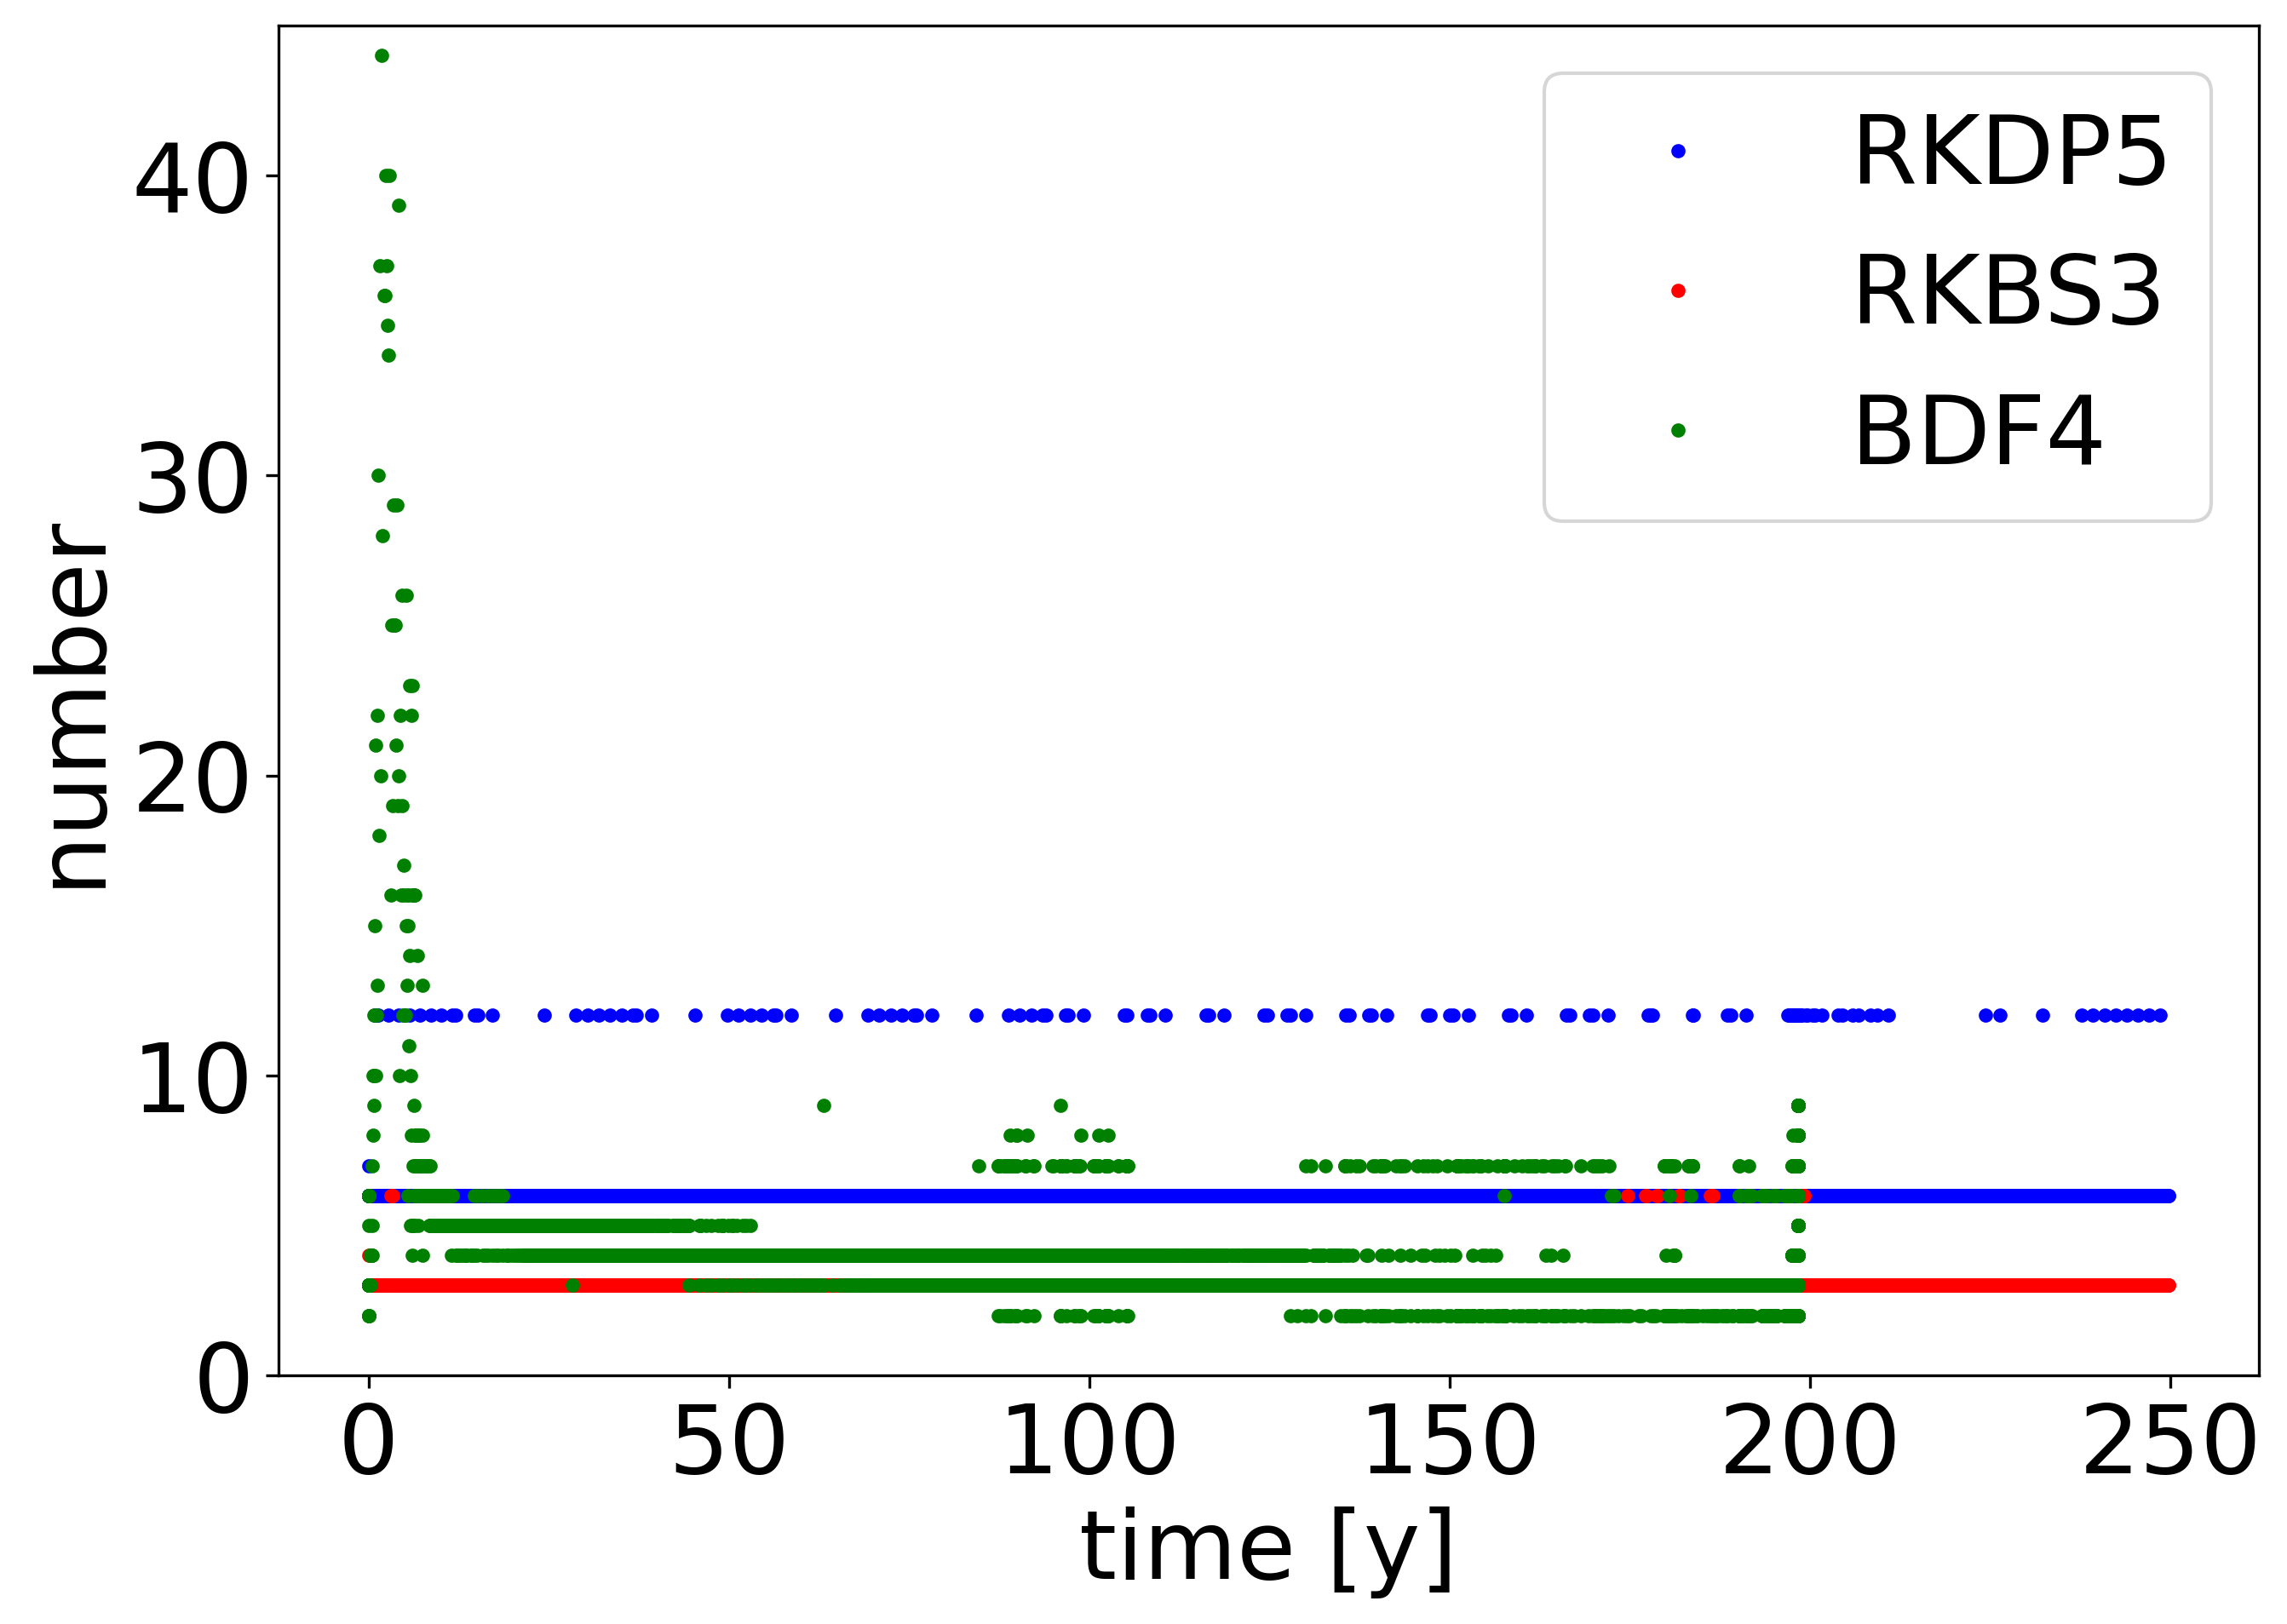
\includegraphics[width=1\textwidth]{images/TANDEMtimeEvolutionRHSall.png}
       	\subcaption{Full simulation time} 
    \end{subfigure}
    \begin{subfigure}{0.32\textwidth}
    	\centering
    	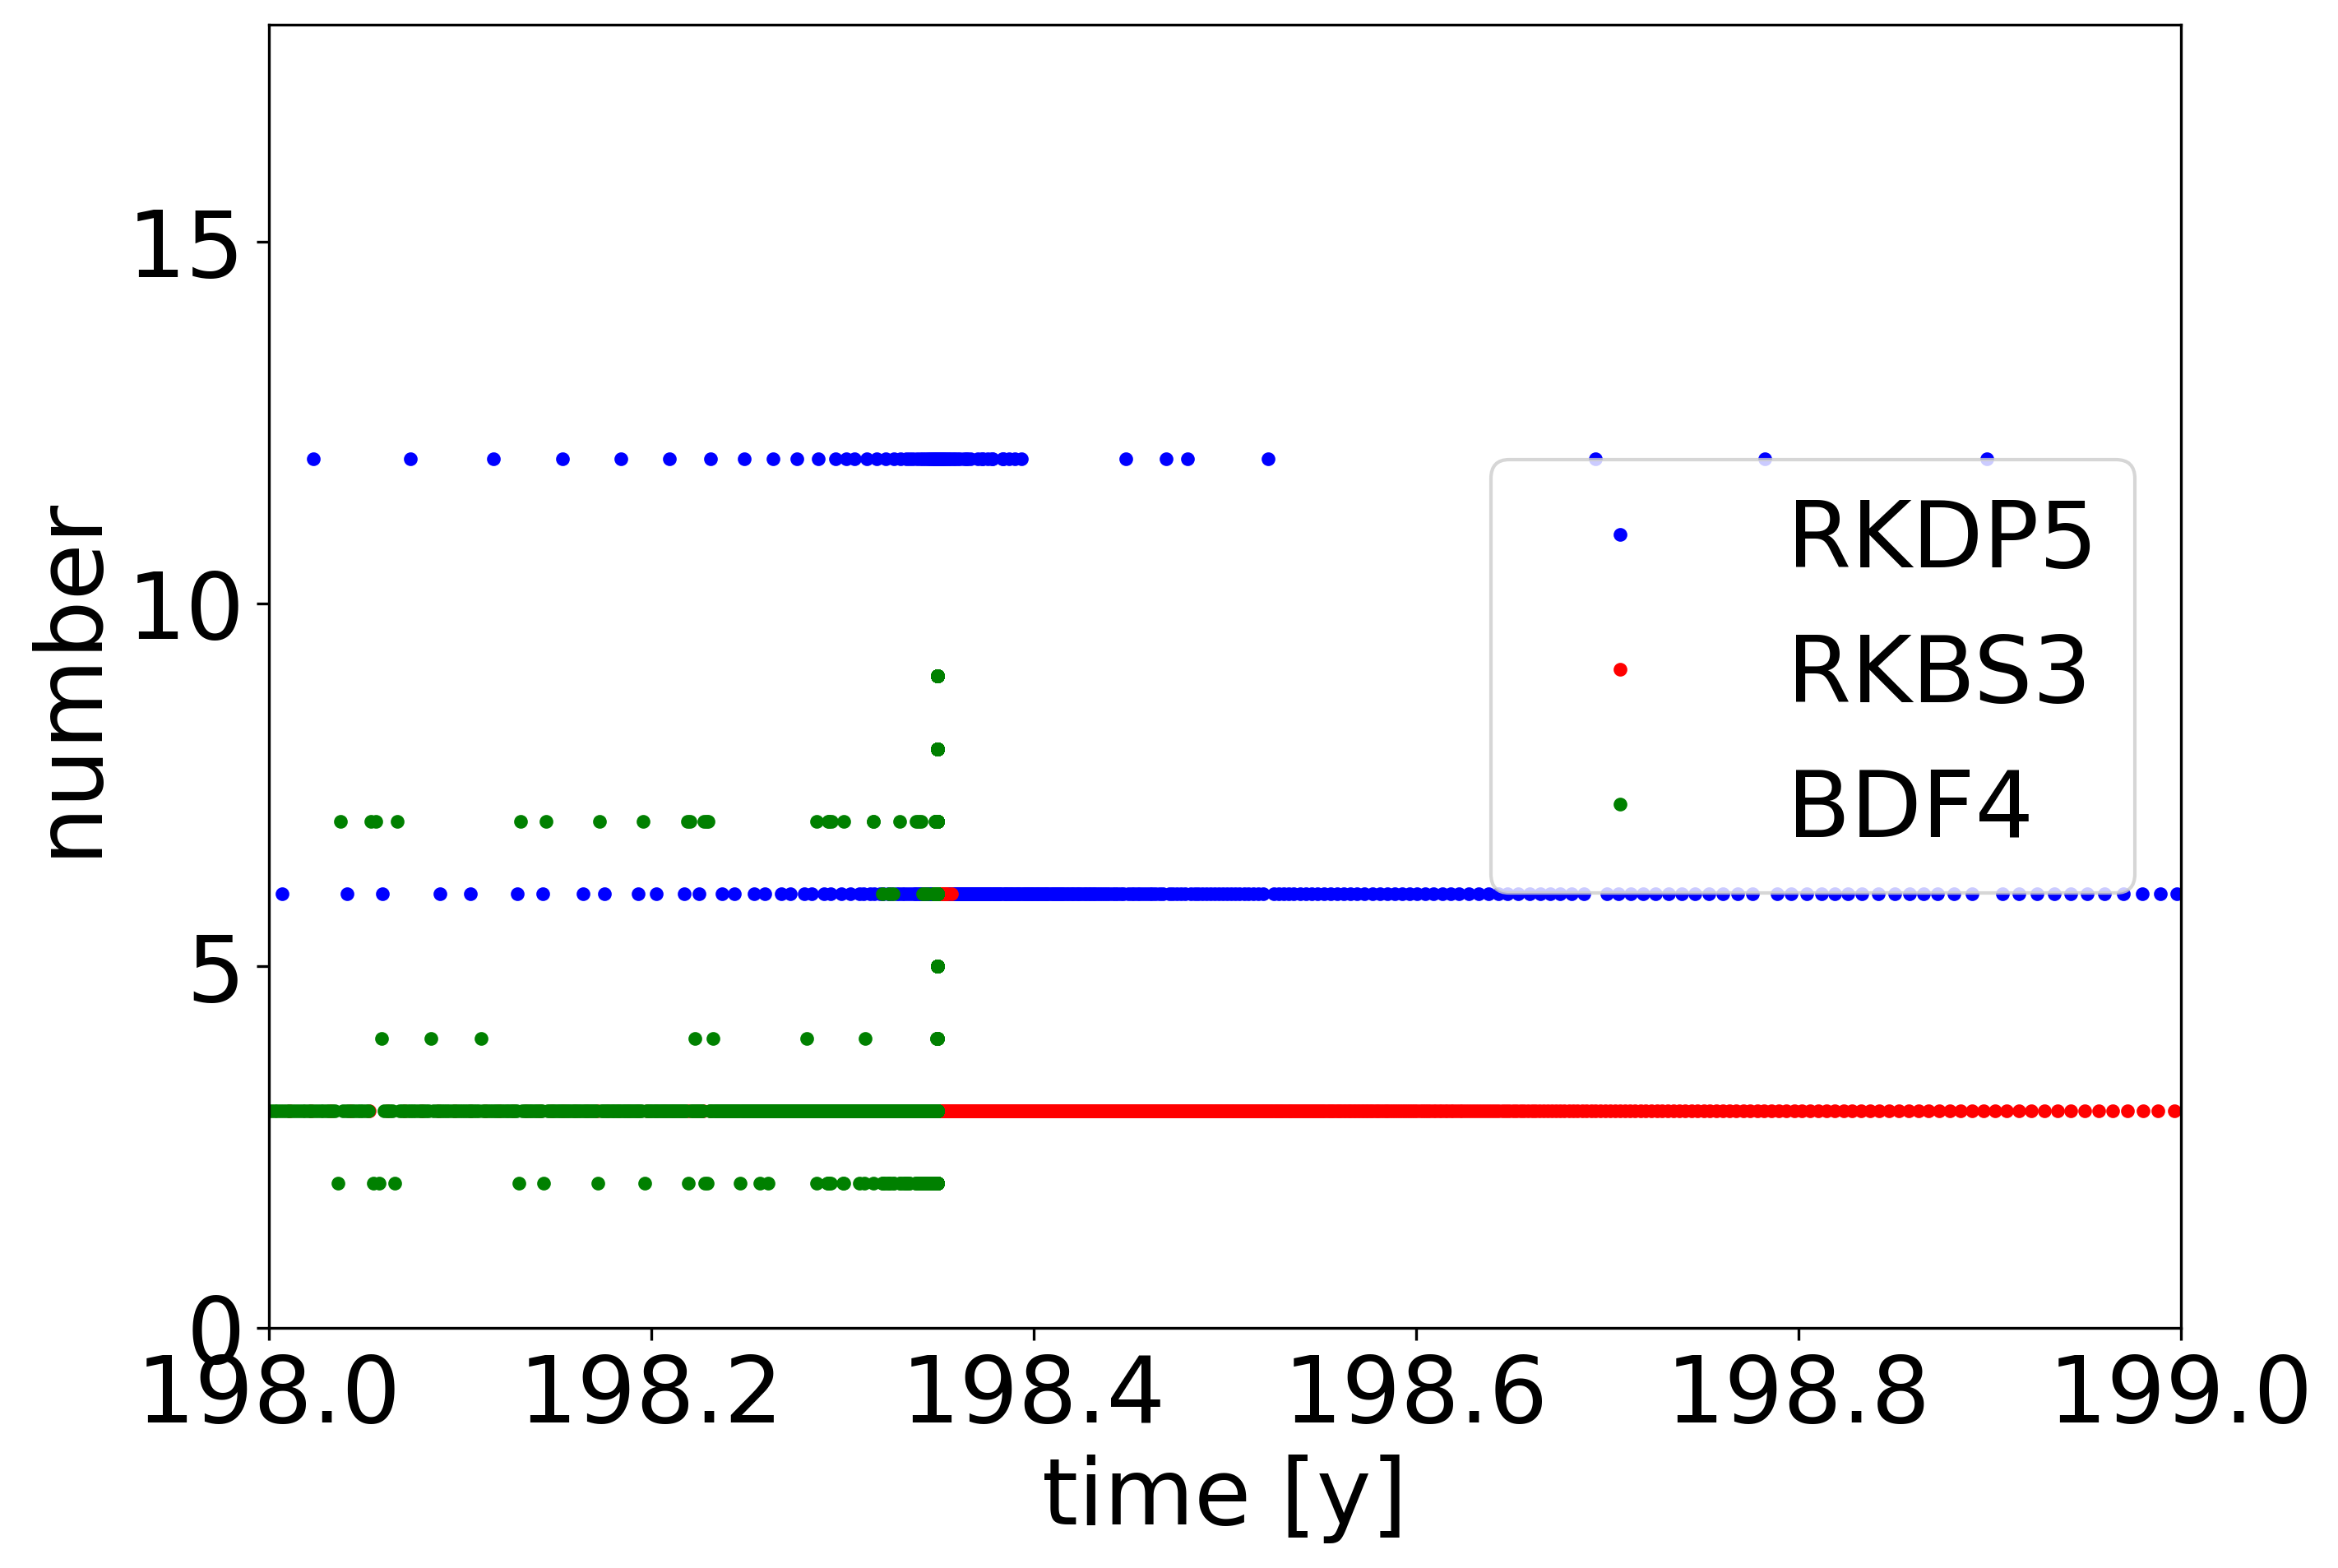
\includegraphics[width=1\textwidth]{images/TANDEMtimeEvolutionRHSsurroundings.png}
       	\subcaption{Year of the earthquake} 
    \end{subfigure}
    \begin{subfigure}{0.32\textwidth}
    	\centering
    	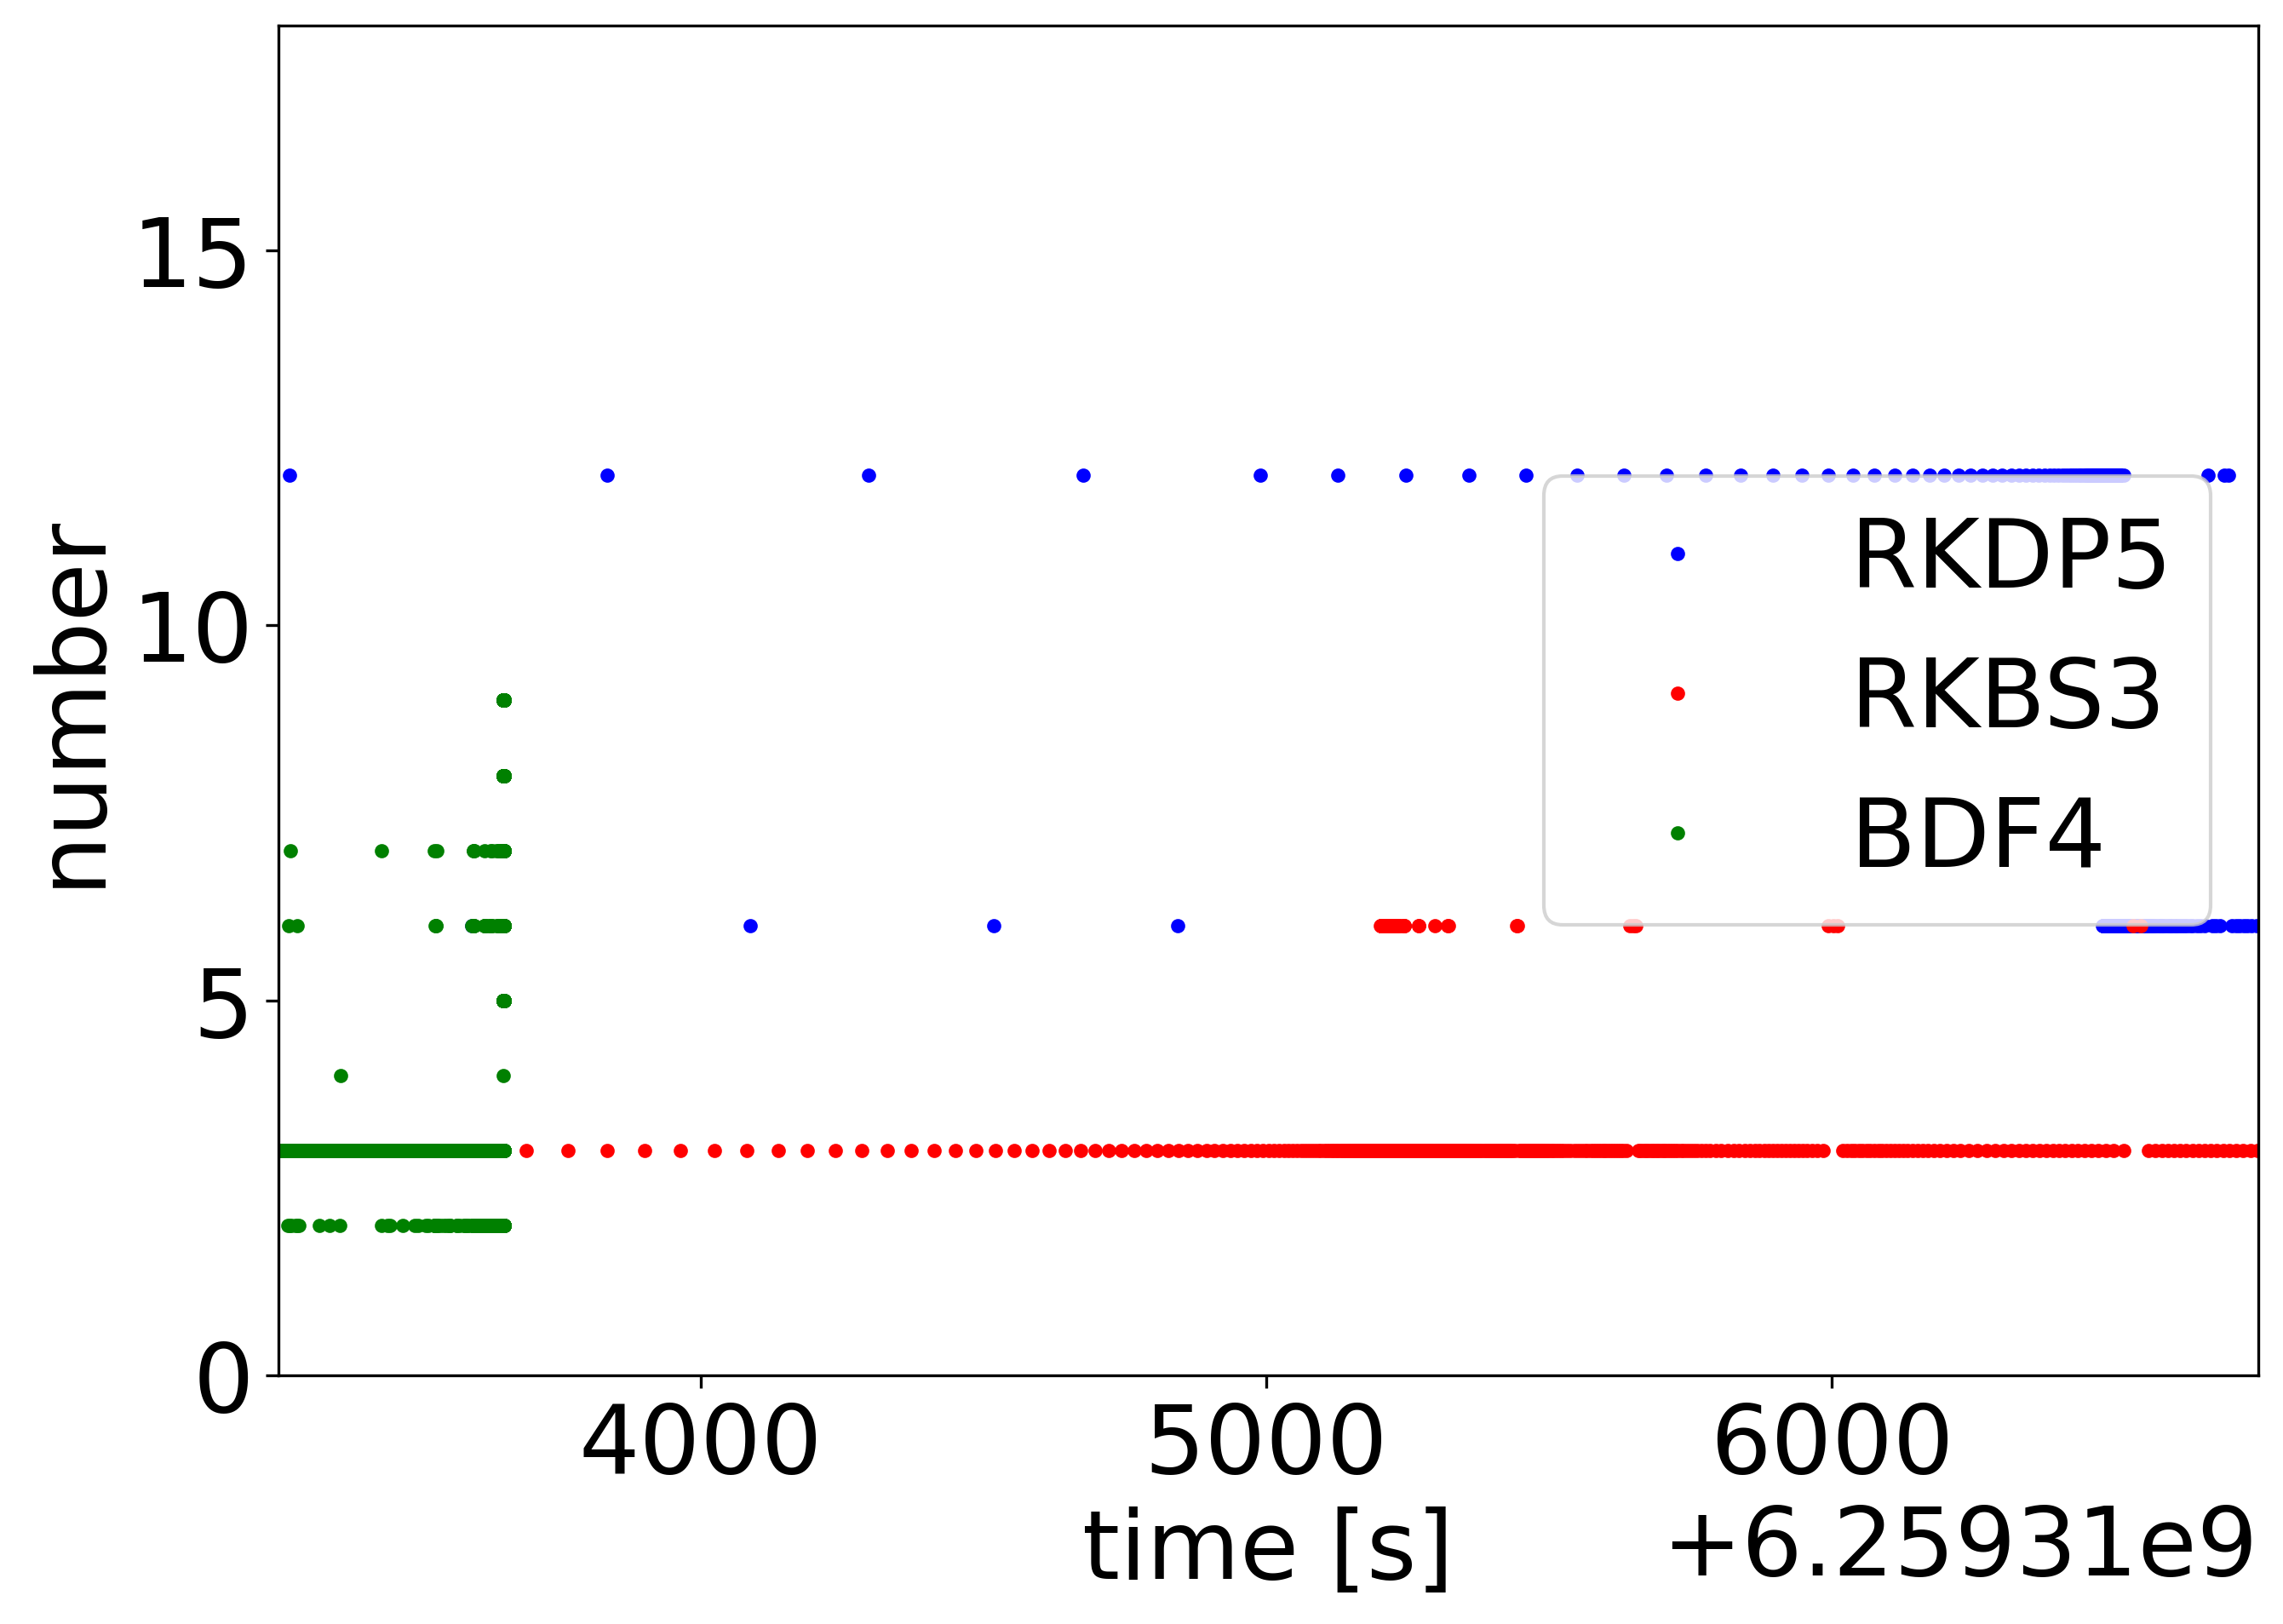
\includegraphics[width=1\textwidth]{images/TANDEMtimeEvolutionRHSearthquake.png}
       	\subcaption{Evolution of the earthquake event} 
    \end{subfigure}
    \caption{Number of evaluations of the right hand side of the ODE in each time iteration for different solvers on the symmetric two-dimensional BP1 problem with 200 elements on the fault}
    \label{fig:timeEvolutionTANDEM_RHS}
\end{figure}

\section{Relative and Absolute Tolerances}
\subsection{Behaviour of the Error}
Tolerances play a crucial role fort adaptive time-stepping methods. A proposed timestep is accepted only if the estimated error is inferior to a defined tolerance $t$, therefore a carefully chosen tolerance has a direct impact on the timestep size and consequently on the total number of time iterations to reach the final simulation time. If $u_i$ refers to all components of the solution vector and $u_i^{(e)}$ to the components of the embedded solution used for the error estimate, then a step is acceptable is following condition is fulfilled: 
\begin{equation}
    \left\|\frac{u_i - u_i^{(e)}}{t_i}\right\|_\infty = \max_i \left|\frac{u_i - u_i^{(e)}}{t_i}\right|
    \quad \leq \quad 1
\end{equation}
The infinity norm is used because a too large deviation in one node of the fault can erroneously provoke an earthquake at a too early time and thus strongly affects the accuracy of the results for the whole system. If the 2-norm was used, as it is common for other applications, too large errors at some nodes may occur, which are then compensated by nodes where the actual and the embedded solutions match well. \\
The tolerance $t_i$ can be defined independently for each component of the solution vector. It is calculated for each time step with an absolute tolerance $t_i^a$ and a relative tolerance $t_i^r$. 
\begin{equation}
    t_i = t_i^a + \max\left(u_i,u_i^{(e)}\right)t_i^r
\end{equation}
Since some components of the solution vector correspond to the values of the state variable $\psi$ and the other components correspond to the slip $S$, it is appropriate to use two different tolerances for the respective quantities. Thus, $t_i^a$ and $t_i^r$ take the values $t_\psi^a$ and $t_\psi^r$ in case the component at index $i$ refers to the state variable and the values $t_S^a$ and $t_S^r$ if the index $i$ refers to the slip at the fault. The motivation behind this decision can be seen in \autoref{fig:errrors1e-7}, which depicts the maximal absolute and relative errors ($\max_i\left|u_i-u_i^{(e)}\right|$ and $\max_i\left|\frac{u_i-u_i^{(e)}}{u_i}\right|$) for the respective components of $\psi$ and $S$. For this simulation, all errors have been set to $t_i^r = t_i^a = 10^{-7}$, without any distinction between slip or state variable components nor between relative or absolute tolerances.
\begin{figure}[H]
    \centering
    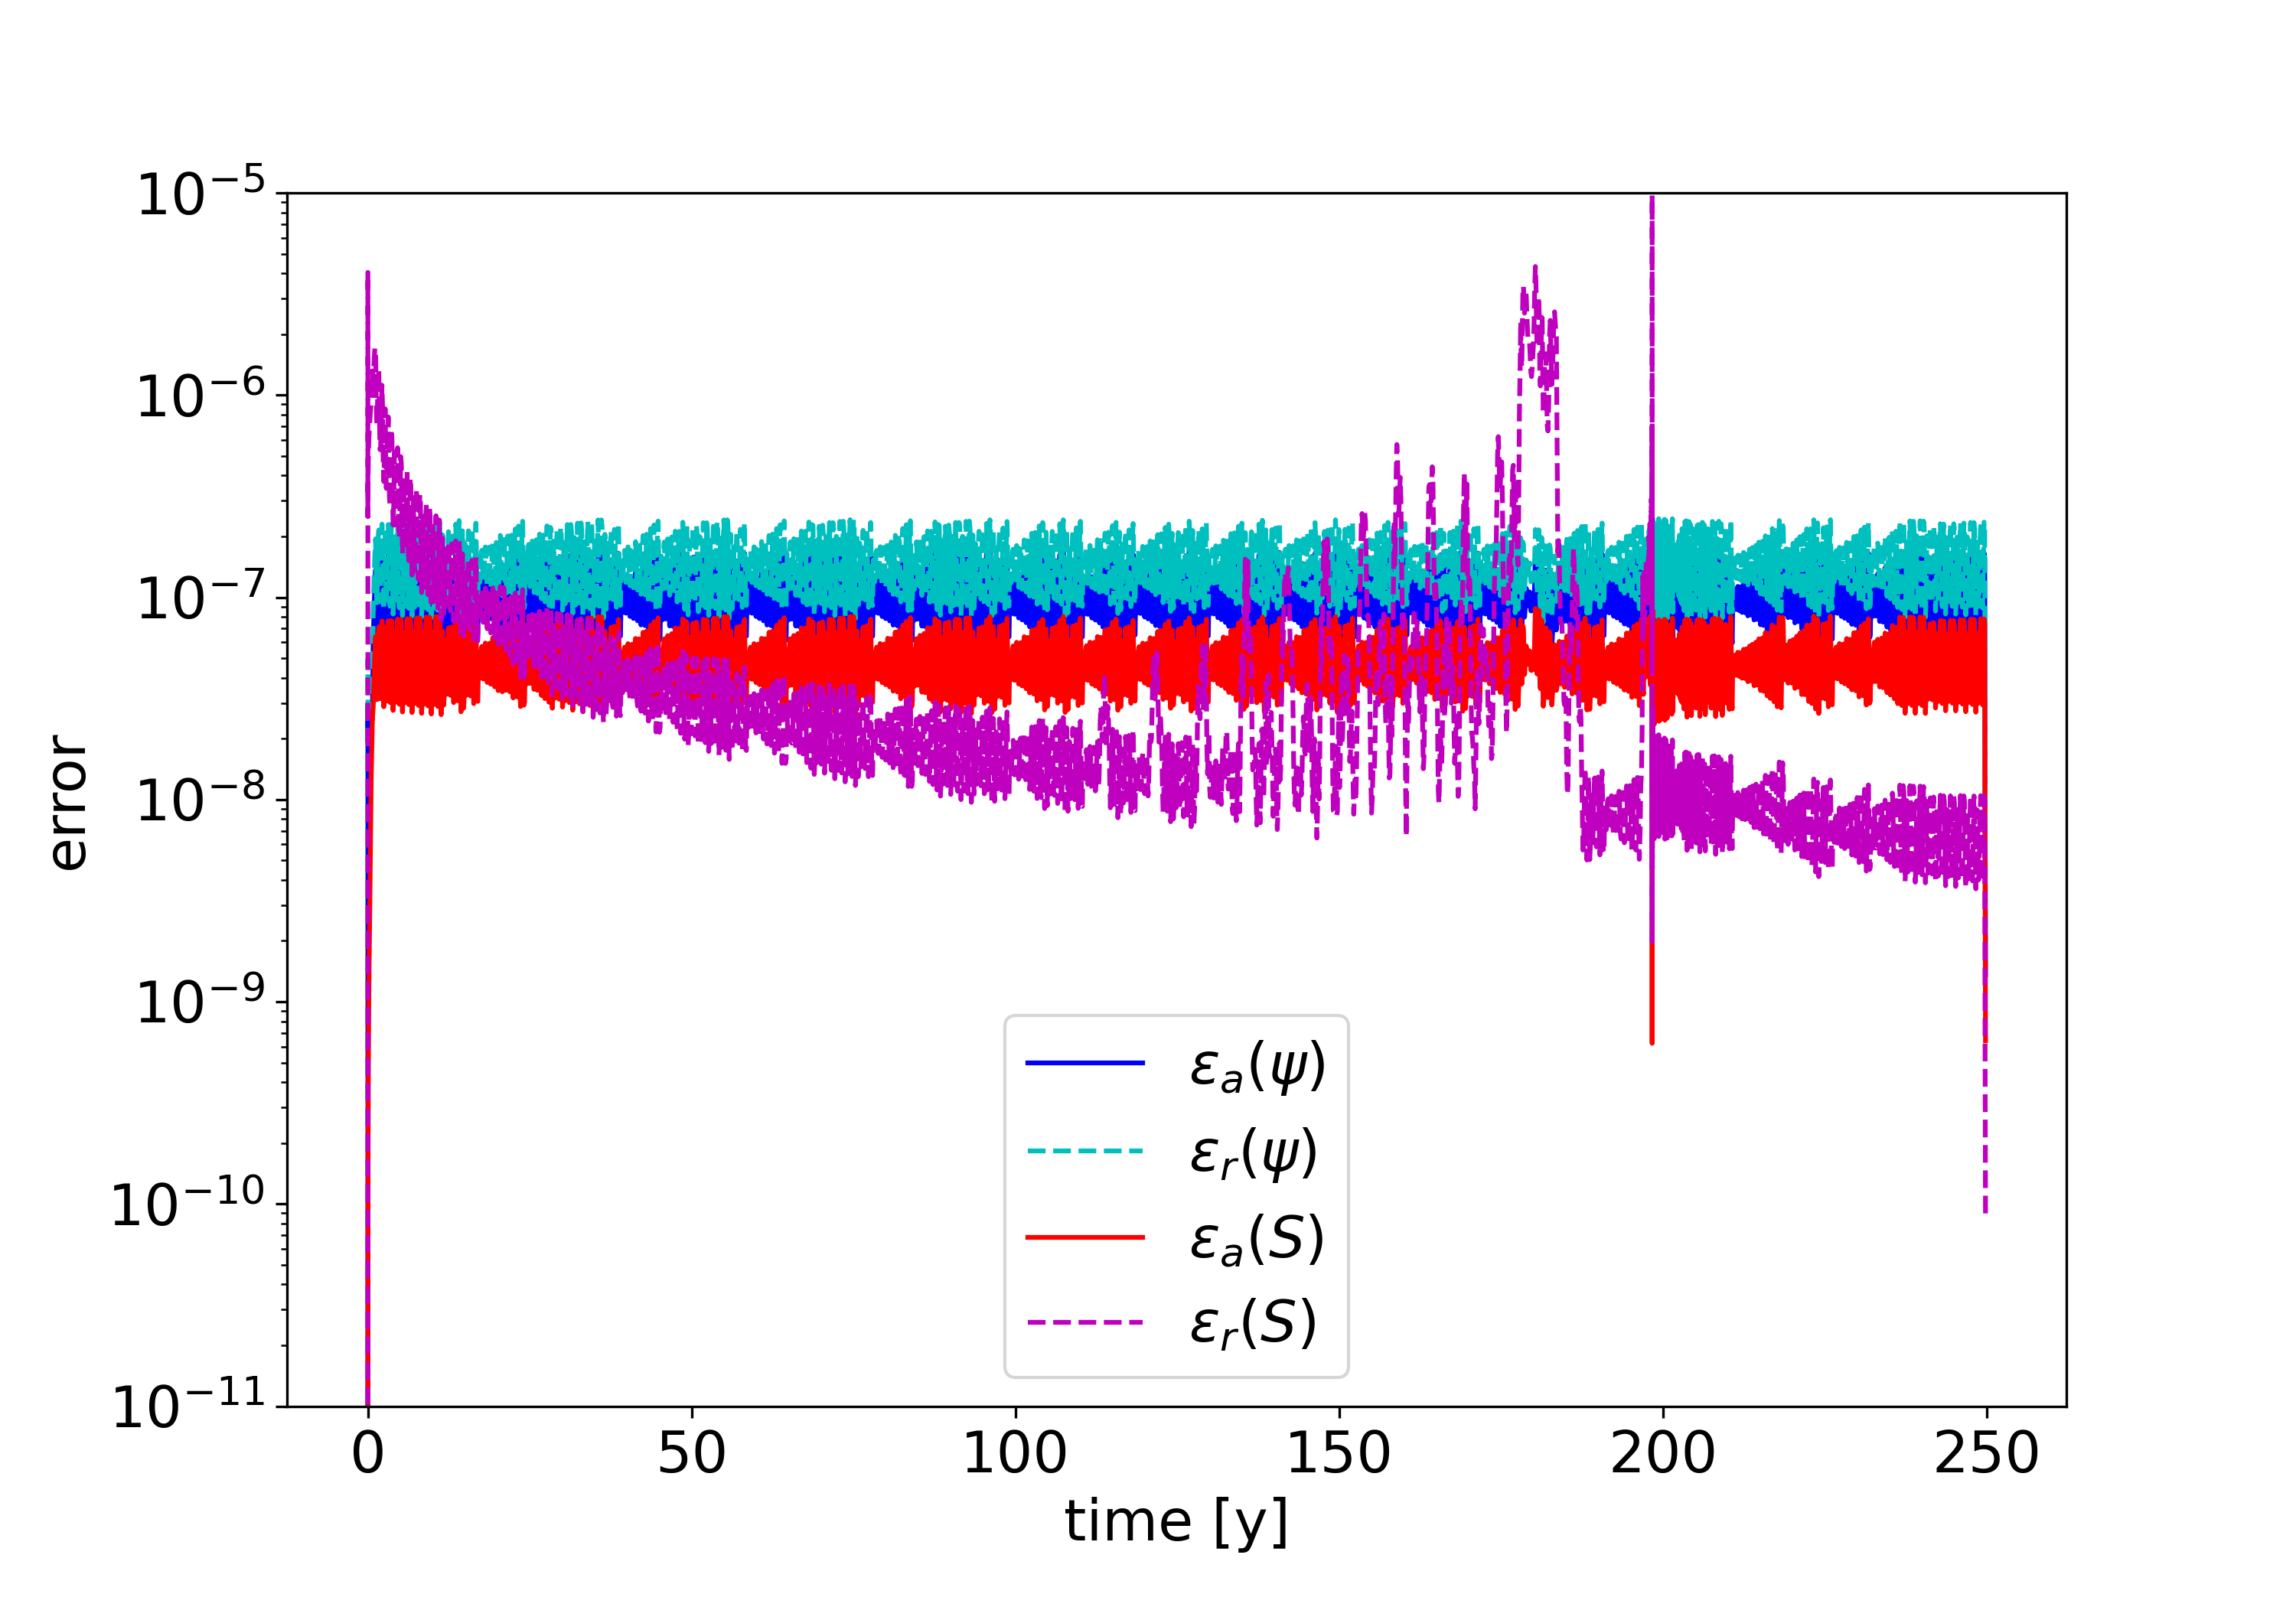
\includegraphics[width=0.6\textwidth]{images/TANDEMtimeEvolutionErrorall_RKDP5.png}
    \caption{Maximum relative and absolute errors using the RKDP5 method on a fault with 200 elements with an absolute and relative error tolerance of $10^{-7}$}
    \label{fig:errrors1e-7}
\end{figure}
Over the whole simulation time, the state variable $\psi$ takes values close to $0.8$ on all fault nodes, leading to a total tolerance for the corresponding components of $t_\psi \approx 1.8 \cdot 10^{-7}$. The blue line, which draws the maximum absolute error, is clearly limited by this tolerance value and the light blue line of the relative error is located, as expected, by a factor $1/0.8$ above the absolute error. \\
The error analysis of the slip presents a much less regular picture. The maximal absolute error lies always below the tolerance $t_S^a = 10^{-7}$, however the relative error reaches much higher values at the beginning of the simulation and before the earthquake event. The evolution of the extreme values of the slip in \autoref{fig:minmax1e-7} provides an explanation for these large errors. In the beginning, the slip at each node is below 1, thus the overall tolerance \\

\begin{figure}[H]
    \centering
    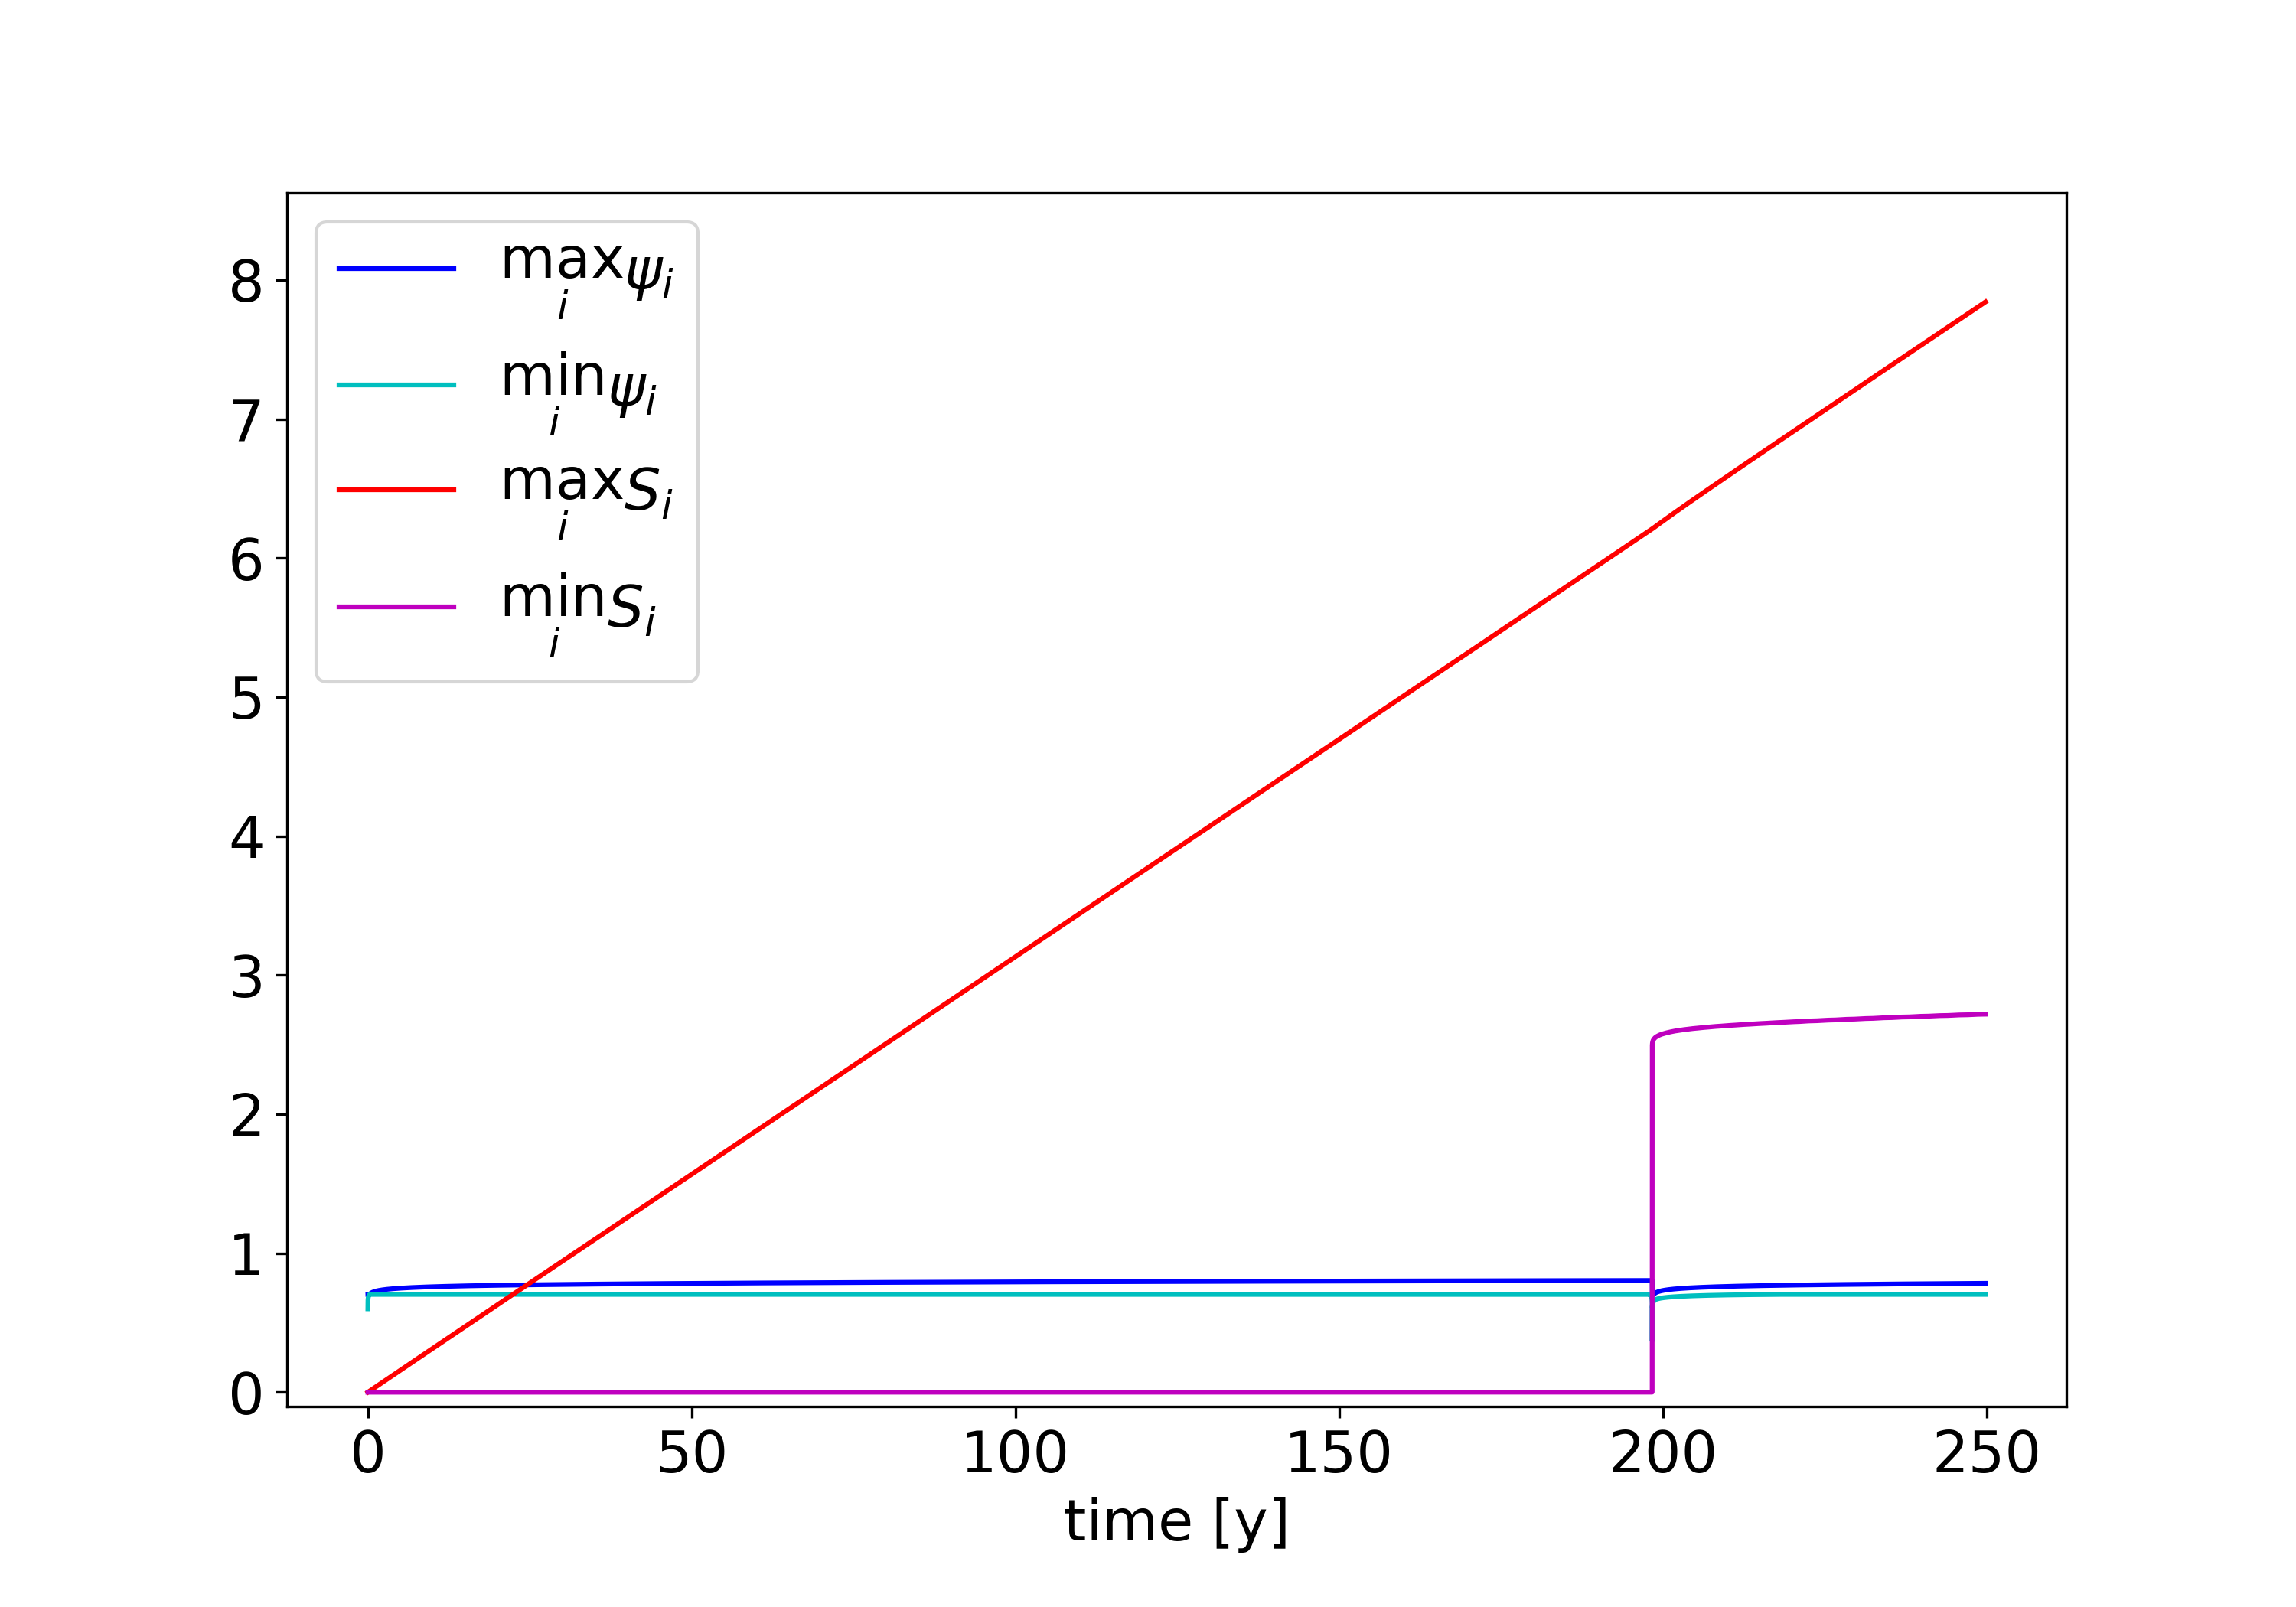
\includegraphics[width=0.6\textwidth]{images/TANDEMtimeEvolutionMinMaxAll_RKDP5.png}
    \caption{Maximum and minimum values of the state variable $\psi$ and of the slip $S$ over time. Simulation performed with the RKDP5 method on a fault with 200 elements with an absolute and relative error tolerance of $10^{-7}$}
    \label{fig:minmax1e-7}
\end{figure}

\subsection{Tolerance of the State Variable Dependent on the Slip}
Overall, the absolute error of the slip is inferior to the absolute error of the state variable. From a physical point of view, the slip is a relevant quantity to describe earthquakes whereas the state variable $\psi$ is only required to solve the DAE. Therefore, the absolute and relative tolerances are defined as external requirements for the slip only, and the tolerances for the state variable have to be chosen in a way to achieve the best numerical performance without loosing physical accuracy. In the following equations, we try to evaluate the highest acceptable tolerances for the state variable in function of the provided tolerances for the slip. The relation between $S$ and $\psi$ is described by the friction law in \autoref{eq:SEASDAE_frictionLaw}, which is evaluated at a constant velocity $V^*$. For a maximal absolute slip error $\epsilon_S^a$, the largest acceptable absolute error of the state variable $\epsilon_\psi^a$ can be calculated by equalizing the induced error in the friction law under constant velocity. 
\begin{align}
    f_{V^*}(S+\epsilon_S^a,\psi) - f_{V^*}(S,\psi) &= f_{V^*}(S,\psi+\epsilon_\psi^a) - f_{V^*}(S,\psi) \\
    \tau(U(S+\epsilon_S^a)) - \tau(U(S)) &= a \sigma_n \text{arsinh}\left(\frac{V^*}{2V_0}\right)\frac{1}{a}\left(e^{\frac{\psi+\epsilon_\psi^a}{a}} - e^{\frac{\psi}{a}}\right) \\
    \tau(B(S+\epsilon_S^a)) - \tau(BS) &= a \sigma_n \text{arsinh}\left(\frac{V^*}{2V_0}\right) e^{\frac{\psi}{a}}\left(e^{\frac{\epsilon_\psi^a}{a}} - 1\right)
\end{align}

As already discussed in the formulation of the Jacobian matrix, the displacement $U(S)$ is linear in $S$ and can therefore be expressed with the linear transformation matrix $B$ as $U(S) = BS$. Further transformations of the left side of the equation are performed in index notation, where $\mathbbm{1}$ denotes a vector in which all components are equal to one. 
\begin{align}
    (\nabla u(S))_{pq} =& \frac{1}{2}\left(D_{lpq}^0u_l^0 + D_{lpq}^1u_l^1\right) + c_0\left(E_{lq}^0u_l^0 - E_{lq}^1u_l^1 - f_q\right)n_{pq} \\ \nonumber
    (\nabla u(S + \epsilon_S^a))_{pq} =& \frac{1}{2}\left(D_{lpq}^0\left(u_l^0+ B_{lj}\mathbbm{1}_j\epsilon_S^a\right) + D_{lpq}^1\left(u_l^1+ B_{lj}\mathbbm{1}_j\epsilon_S^a\right)\right) \\ &+ c_0\left(E_{lq}^0\left(u_l^0+ B_{lj}\mathbbm{1}_j\epsilon_S^a\right) - E_{lq}^1\left(u_l^1+ B_{lj}\mathbbm{1}_j\epsilon_S^a\right) - f_q\right)n_{pq} \\
    (\nabla u(S + \epsilon_S^a))_{pq} - (\nabla u(S))_{pq} =& \left(\frac{1}{2}\left(D_{lpq}^0 + D_{lpq}^1\right) + c_0\left(E_{lq}^0 - E_{lq}^1\right)n_{pq}\right)B_{lj}\mathbbm{1}_j\epsilon_S^a \\
    \tau_p(B(S+\epsilon_S^a)) - \tau_p(BS) =& M_{rp}^{-1}e_{qr}^Tw_q\left((\nabla u(S + \epsilon_S^a))_{kq} - (\nabla u(S))_{kq}\right)n_{kq}
\end{align}
We can see that the error in $\tau$ does not depend on the slip $S$ anymore and is proportional to the absolute slip error $\epsilon_S^a$. We can thus define a matrix $C$ such that $\tau_p(B(S+\epsilon_S^a)) - \tau_p(BS) = C_{pj}\mathbbm{1}_j\epsilon_S^a$. The absolute error of the state variable is then directly proportional to $\epsilon_S^a$. 
\begin{align}
    \epsilon_\psi^a &= a\text{ln}\left(1+\frac{C_{pj}\mathbbm{1}_j}{a\sigma_n \text{arsinh}\left(\frac{V^*}{2V_0}\right)e^{\frac{\psi}{a}}}\epsilon_S^a\right) 
\end{align}
To provide an upper bound for $\epsilon_\psi^a$, the smallest value of the proportionality factor of $\epsilon_S^a$ has to be determined because the logarithm function is increasing and the smallest allowed value of the error is searched. For the numerator of the ratio, to calculate $\min_p\left|C_{pj}\mathbbm{1}_j\right|$ minimizes the ratio. Note that the matrix $C$ depends on the geometry so this term cannot be provided in general in beforehand but has to be chosen with respect to the used space discretization. To minimize the ratio, the terms on the denominator have to be maximized. Because the arsinh function increases monotonously, the choice of $V_{max}$ for the velocity component provides an appropriate upper bound. Similarly, $\psi$ should be replaced by an upper limit $\psi_{max}$. The value of the parameter $a$ depends on the fault location and varies between $a_{min}$ and $a_{max}$. It appears once at the beginning of the denominator, where its maximal value shall be chosen, and once in the exponential, where its minimal value is required. If all those values are plugged into the expression, the error in $\psi$ can be evaluated as following: 
\begin{equation}
    \epsilon_\psi^a = a_{min}\text{ln}\left( 1+\frac{\min_p\left|C_{pj}\mathbbm{1}_j\right|}{a_{max}\sigma_n \text{arsinh}\left(\frac{V_{max}}{2V_0}\right) e^{\frac{\psi_{max}}{a_{min}}}}\epsilon_S^a\right)
\end{equation}
The upper bounds for the velocity and for the state variable can be deduced by already obtained simulation results and an appropriate choice could be the values $V_{max} = 5.0ms^{-1}$ and $\psi_{max} = 0.85$. In the simulation settings, $a$ increases from $a_{min}=0.010$ at the surface to $a_{max}=0.025$ at high depths. With these values, all terms take reasonable values, except for the exponential $e^{\frac{\psi_{max}}{a_{min}}} = e^{85} \approx 8\cdot10^{36}$. In the vicinity of 1,  the logarithm can be approximated by a linear function with gradient 1. Under consideration of the initial factor $a_{min}$, the absolute error tolerance in $\psi$ has to be 38 magnitudes below the tolerance in the slip to prevent any additional error. Such a low tolerance is not achievable in any realistic scenario, so the state variable participates in making the simulation less accurate. When the tolerances for the state variable have to be set, and only an absolute tolerance for the slip is provided, it is the best to chose them as low as possible, and still the state variable will contribute to the error of the simulation. On the other hand, very low tolerances prevent the choice of larger timesteps and an appropriate choice of the tolerance for the state variable which is not too low to ensure reasonable execution times still needs to be determined.  

\subsection{Tolerance of the State Variable Dependent on the Slip Rate}
So far, the error in the slip rate $V$ is not directly regulated by any tolerance value. Since it is calculated from the slip and from the state variable, the error in $V$ depends on the chosen tolerances for those two parameters. As a physical quantity, it might be interesting to provide a tolerance for the slip rate too. Unlike for the slip, the tolerance for the slip rate should also include a relative error tolerance $t_V^r$ in addition to the already discussed absolute error tolerance $t_V^a$. Indeed, the slip rate takes values around $10^{-6}ms^{-1}$ in the aseismic phase and peaks at values above $10^{9}ms^{-1}$ during the earthquake event. The exclusive use of an absolute error tolerance, with a value below the slip rate of the aseismic evolution, is too restrictive during the earthquake. An appropriate relative error tolerance, which is scaled by the current velocity value and added to the absolute one can reasonably restrict the error. In the aseismic phase, the relative error tolerance does not have much effect since it is scaled down by the very low slip rate and outmatched by the presumably higher absolute tolerance. For example, the choices $t_V^a=10^{-10}$ and $t_V^r=10^{-7}$ allow for a relative error of the order $10^{-4}$ during the aseismic phase and of the order $10^{-7}$ during the earthquake. Such a choice reflects the concept that a higher accuracy is needed to simulate an earthquake than to simulate aseismic slip. \\
The typical approach would be to estimate it with the difference between the values obtained from the numerical solution and its embedded solution. The newly chosen timestep shall then only allow solutions which fulfill the tolerances in the entire state vector and the additional tolerance in error of the slip rate. Alternatively, the error tolerance of the state variable, which is not properly defined from physical constrains yet can be used to restrict the slip rate. To obtain the relation between error in slip rate $V$ and state variable $\psi$, the same analysis as in the previous subsection has to be performed. This time, the error in the friction law is evaluated under the assumption of a constant slip $S^*$.  
\begin{align}
	f_{S^*}(V+\epsilon_V^a,\psi) - f_{S^*}(V,\psi) &= f_{S^*}(V,\psi+\epsilon_\psi^a) - f_{S^*}(V,\psi) \\
	 f_{S^*}(V,\psi) + \frac{d}{dV}f_{S^*}(V,\psi)\epsilon_V^a - f_{S^*}(V,\psi) + \mathcal{O}\left(\left(\epsilon_V^a\right)^2\right)&= a \sigma_n \text{arsinh}\left(\frac{V}{2V_0}\right)\frac{1}{a}\left(e^{\frac{\psi+\epsilon_\psi^a}{a}} - e^{\frac{\psi}{a}}\right) \\
	 \left( \frac{a\sigma_ne^{\frac{\psi}{a}}} {2V_0\sqrt{\left(\frac{V}{2V_0}\right)^2+1}}- \eta \right)\epsilon_V^a + \mathcal{O}\left(\left(\epsilon_V^a\right)^2\right) &= a \sigma_n \text{arsinh}\left(\frac{V}{2V_0}\right) e^{\frac{\psi}{a}}\left(e^{\frac{\epsilon_\psi^a}{a}} - 1\right)
\end{align}
\begin{equation}
	 \epsilon_\psi^a 
	= a\text{ln}\left(1 + \left( \frac{1}{\text{arsinh}\left(\frac{V}{2V_0}\right)\sqrt{V^2 + (2V_0)^2}} - \frac{\eta}{a \sigma_n \text{arsinh}\left(\frac{V}{2V_0}\right) e^{\frac{\psi}{a}}} \right)\epsilon_V^a + \mathcal{O}\left(\left(\epsilon_V^a\right)^2\right)\right)
\end{equation}
The exponential $e^{\frac{\psi}{a}}$ with the extremely high value appears again in one of the two ratios. The term with $\eta$ can thus be neglected to estimate the error. In the remaining summand, an appropriate estimate value for the slip rate $V$ needs to be determined. As stated previously, the absolute error tolerance is only relevant for the aseismic phase, in which the slip rate never exceeds the tectonic slip $V_0$, which can be taken as an upper bound for the slip rate here. The absolute error is then calculated by: 
\begin{equation}
	\label{eq:absoluteErrorPSIFromV}
	 \epsilon_\psi^a 
	= a_{min}\text{ln}\left(1 +  \frac{1}{\text{arsinh}\left(\frac{1}{2}\right)\sqrt{5}V_0}\epsilon_V^a\right)
\end{equation}
During an earthquake, the relative error tolerance of the slip rate is relevant. To evaluate it, we now investigate the relation between the relative errors of the slip rate and the state variable. 
\begin{align}
	f_{S^*}((1+\epsilon_V^r)V,\psi) - f_{S^*}(V,\psi) &= f_{S^*}(V,(1+\epsilon_\psi^r)\psi) - f_{S^*}(V,\psi) \\
	f_{S^*}(V,\psi) + \frac{d}{dV}f_{S^*}(V,\psi)\epsilon_V^rV - f_{S^*}(V,\psi) + \mathcal{O}\left(\left(\epsilon_V^rV\right)^2\right)&= a \sigma_n \text{arsinh}\left(\frac{V}{2V_0}\right)\frac{1}{a}\left(e^{\frac{(1+\epsilon_\psi^r)\psi}{a}} - e^{\frac{\psi}{a}}\right) \\
	\left( \frac{a\sigma_ne^{\frac{\psi}{a}}} {2V_0\sqrt{\left(\frac{V}{2V_0}\right)^2+1}}- \eta \right)\epsilon_V^rV + \mathcal{O}\left(\left(\epsilon_V^rV\right)^2\right) &= a \sigma_n \text{arsinh}\left(\frac{V}{2V_0}\right) e^{\frac{\psi}{a}}\left(e^{\frac{\epsilon_\psi^r}\psi{a}} - 1\right)
\end{align}
\begin{equation}
	\epsilon_\psi^r = \frac{a}{\psi}\text{ln}\left(1 + \left( \frac{1}{\text{arsinh}\left(\frac{V}{2V_0}\right)\sqrt{V^2 + (2V_0)^2}} - \frac{\eta}{a \sigma_n \text{arsinh}\left(\frac{V}{2V_0}\right) e^{\frac{\psi}{a}}} \right)\epsilon_V^rV + \mathcal{O}\left(\left(\epsilon_V^rV\right)^2\right)\right)
\end{equation}
Again, the term with $\eta$ can be neglected because of the exponential. For elements, where the relative tolerance is relevant, the slip rate is much larger than the tectonic slip, so $V_0^2$ can also be neglected below the square root when added to $V^2$. The relative error in $\psi$ can be estimated as: 
\begin{equation}
	\label{eq:relativeErrorPSIFromV}
	\epsilon_\psi^r = \frac{a_{min}}{\psi_{max}}\text{ln}\left(1 + \frac{1}{\text{arsinh}\left(\frac{V_{max}}{2V_0}\right)}\epsilon_V^r\right)
\end{equation}

The absolute and relative errors in $\psi$ associated to the respective errors in the slip rate are represented in \autoref{fig:RelAbsErrorToleranceVPSI}. The curves show the evaluation of \autoref{eq:absoluteErrorPSIFromV} and \autoref{eq:relativeErrorPSIFromV} for small error values in $V$. The various parameters are set to $a_{min}=0.01$, $\psi_{max}=0.85$, $V_0=10^{-6}ms^{-1}$ and $V_{max}=5.0ms^{-1}$. To use the previous example again, if an absolute error tolerance in the slip rate of $t_V^a=10^{-10}$ and a relative tolerance of $t_V^r=10^{-7}$ are required, it would translate to the tolerances in the state variable to $t_\psi^a=9.29\cdot10^{-7}$ and $t_\psi^r=2.77\cdot10^{-11}$. However, these values cannot be used as such in the simulation, since the assumption that the absolute tolerance can be neglected during the earthquake and inversely that the relative tolerance is insignificant in the aseismic phase only holds for the slip rate but not for the state variable, whose value remains between $0.75$ and $0.85$. It makes more sense to define an absolute tolerance for the aseismic slip $t_\psi^{as}=9.29\cdot10^{-7}$ and for the earthquake $t_\psi^{eq}=\psi_{min}2.77\cdot10^{-11}=6.48\cdot10^{-11}$ in the state variable. 

\begin{figure}[H]
	\centering
	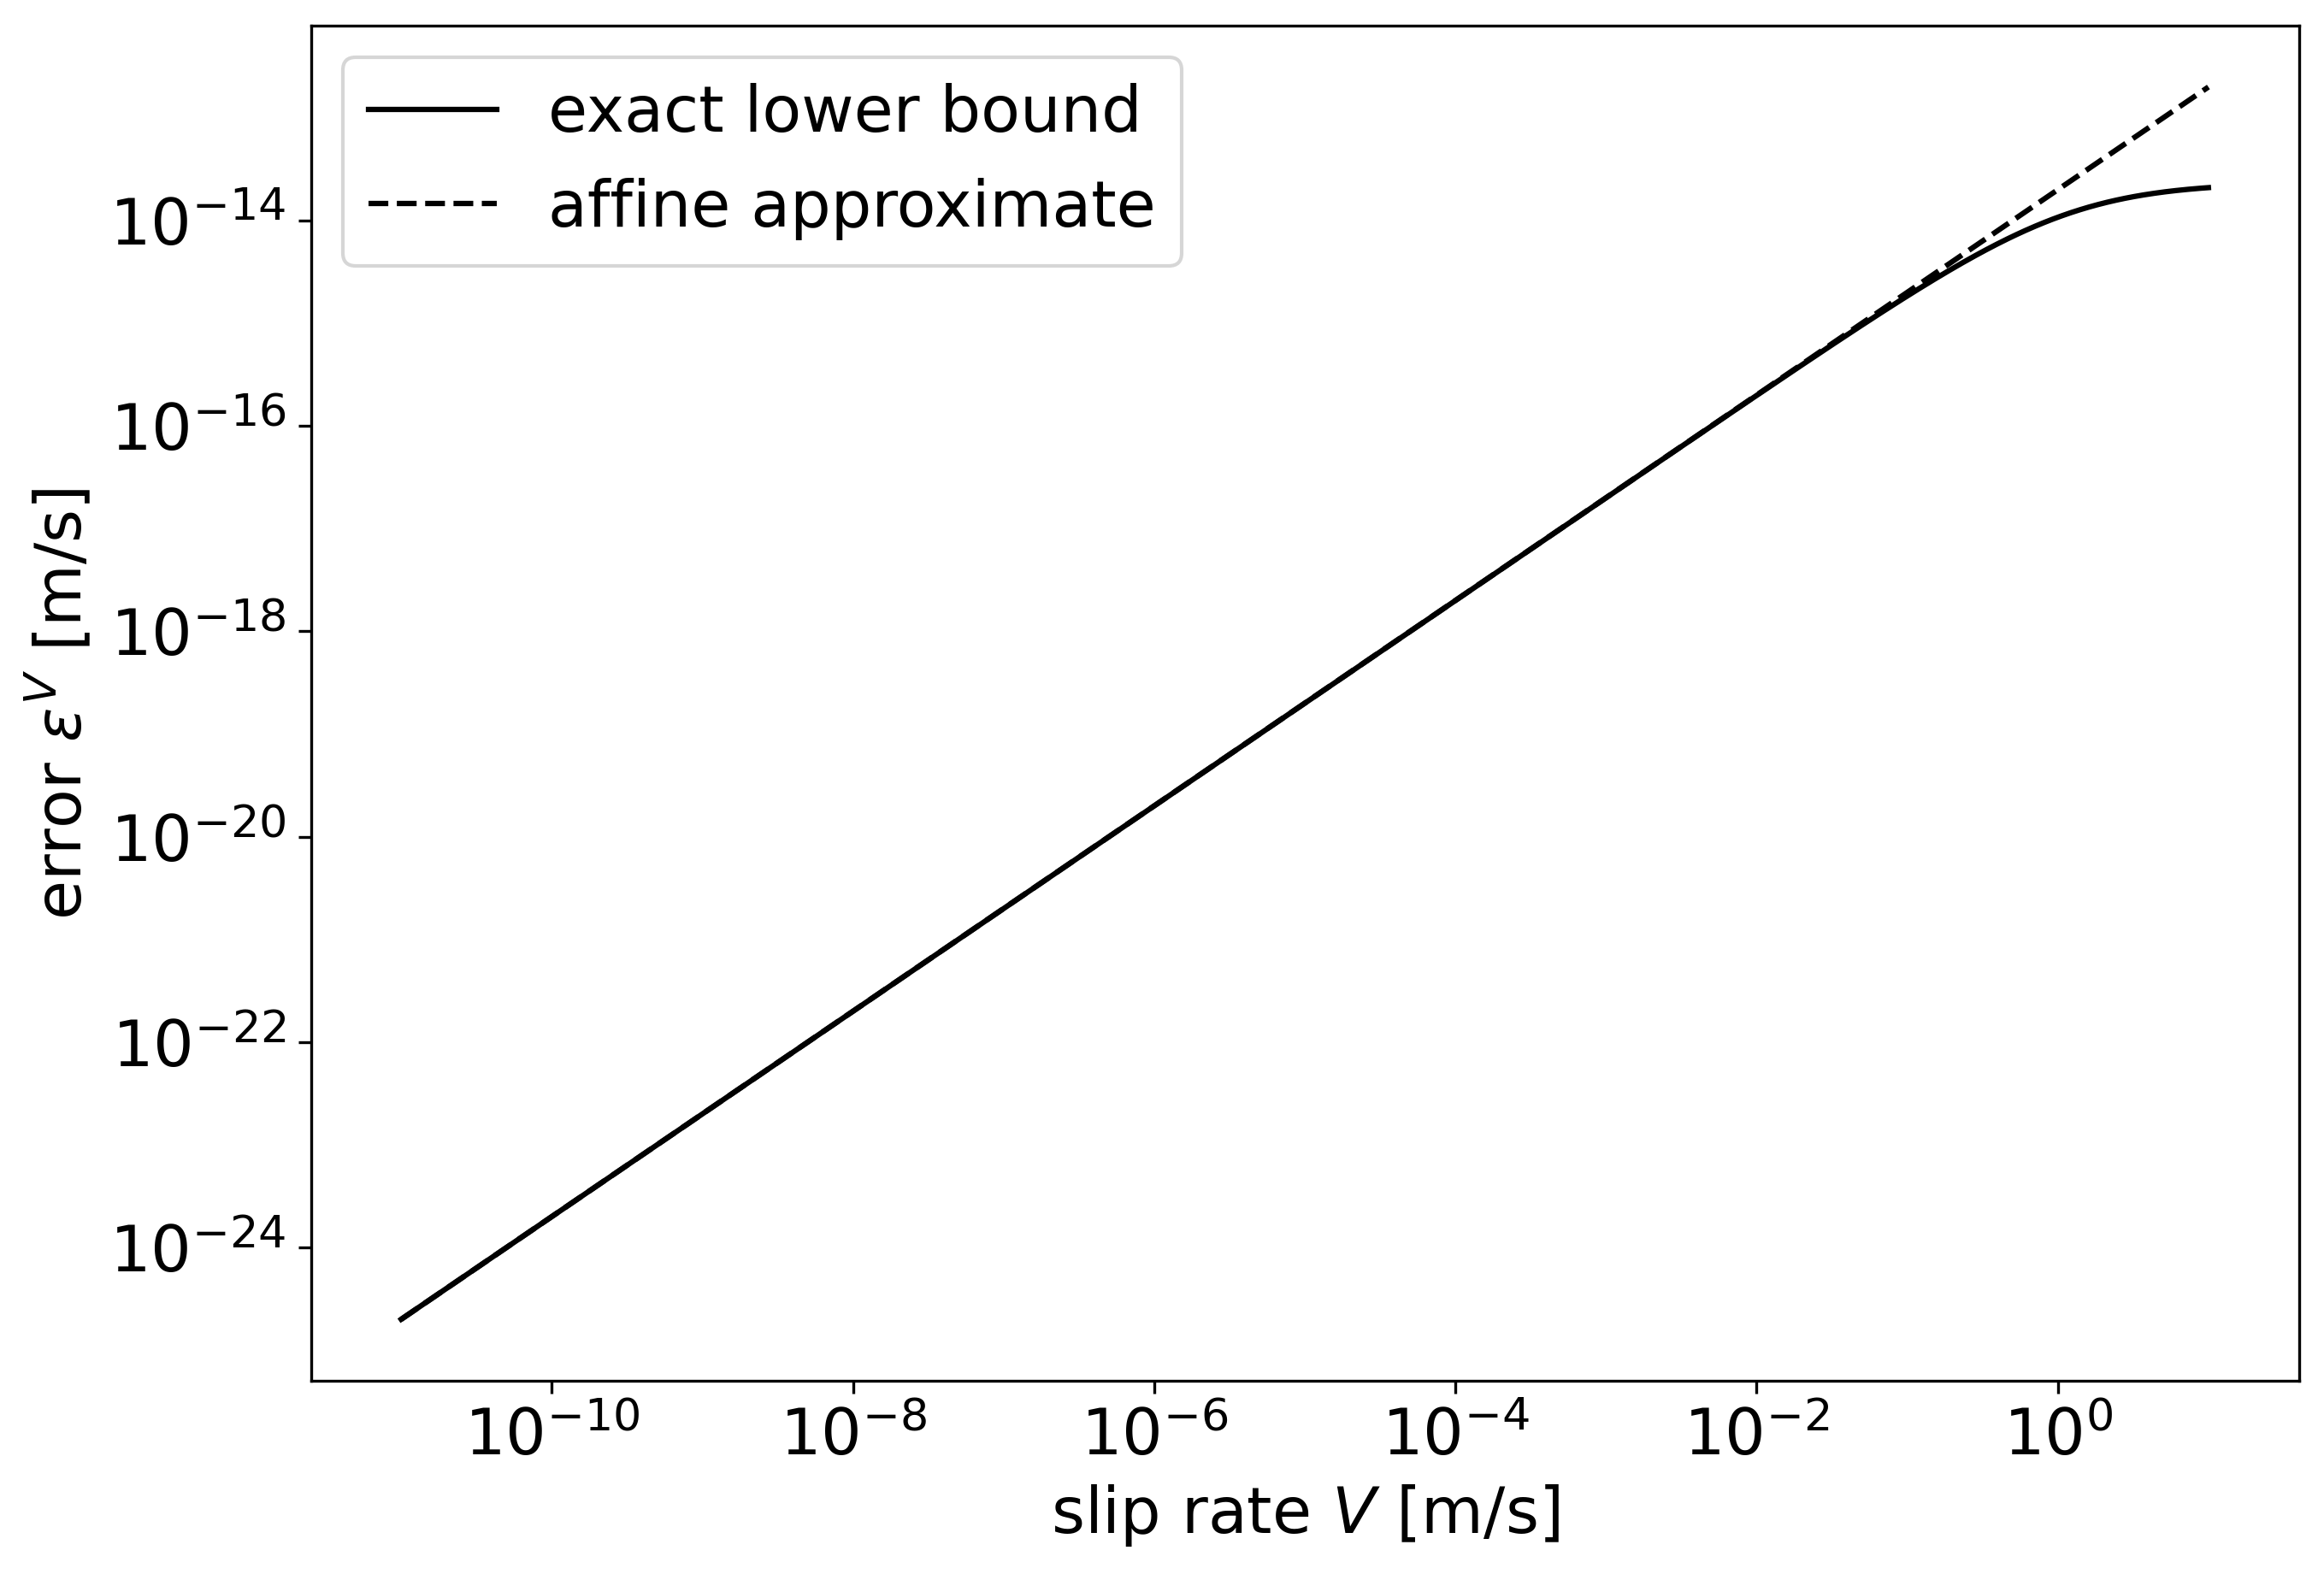
\includegraphics[width=0.6\textwidth]{images/ErrorRelationPSI_VAbsoluteRelative.png}
	\caption{Absolute and relative error in $\psi$ in function of the error in the slip rate}
	\label{fig:RelAbsErrorToleranceVPSI}
\end{figure}

\begin{equation*}
	F(x,y) = 0, y(x) \qquad x\in\mathbb{R}^n, y\in\mathbb{R}^m,F\in\mathbb{R}^m\\
\end{equation*}
\begin{align}
	0 &= \frac{dF_k}{dx_j} = \frac{\partial F_k}{\partial x_i}\frac{dx_i}{dx_j} + \frac{\partial F_k}{\partial y_i}\frac{dy_i}{dx_j} \\
	\frac{dy_i}{dx_j} &= \frac{\partial y_i}{\partial x_l}\frac{dx_l}{dx_j} \\
	\Rightarrow 0 &= \frac{\partial F_k}{\partial x_i}\frac{dx_i}{dx_j} + \frac{\partial F_k}{\partial y_i}\frac{\partial y_i}{\partial x_l}\frac{dx_l}{dx_j}
\end{align}
If the components of $x$ do not depend on each other (no ODE): $\frac{dx_i}{dx_j} = \delta_{ij}$ \\
We obtain exactly the implicit function theorem:
\begin{align}
	0 = \frac{\partial F_k}{\partial x_j} + \frac{\partial F_k}{\partial y_i}\frac{\partial y_i}{\partial x_j} \\
	\Rightarrow \frac{\partial y}{\partial x} = -\left(\frac{\partial F}{\partial y}\right)^{-1}\frac{\partial F}{\partial x} = -F_y^{-1}F_x
\end{align}
If the components of $x$ depend on each other (autonomous ODE): $\frac{dx_i}{dx_j} \neq \delta_{ij}$ is singular. The problem cannot be solved. \\


\begin{equation}
	\frac{dS_i}{dS_j} = \lim\limits_{h\rightarrow0}\frac{S_i(t+h) - S_i(t)}{S_j(t+h) - S_j(t)} = \lim\limits_{h\rightarrow0}\frac{\frac{S_i(t+h) - S_i(t)}{h}}{\frac{S_j(t+h) - S_j(t)}{h}} = \frac{\lim\limits_{h\rightarrow0}\frac{S_i(t+h) - S_i(t)}{h}}{\lim\limits_{h\rightarrow0}\frac{S_j(t+h) - S_j(t)}{h}} = \frac{\frac{dS_i}{dt}}{\frac{dS_j}{dt}}
\end{equation}


\bibliographystyle{alpha}
\bibliography{literature.bib}

\end{document}
